% Gelfand seminar notes, 1979-80: source pages P000840-P000918.
% English translation (AI-made, checked against the scans), cut page by page from the cumulative working reader A4-reader-chapters01-34-complete-first1527-separated-diplomatic-r46.
% \SourcePage{GELFAND-Pnnnnnn}{label} starts a scanned page; the second argument is the number written
% on the page, if any. Editorial notes give the page, a label and the transcriber's remark; \Unclear
% marks a doubtful reading.
\SourcePage{GELFAND-P000840}{30}
\SourceFigure{GELFAND-P000840}{indexed-lines}{%
\begingroup\color{black}\GelfandFitDiagram{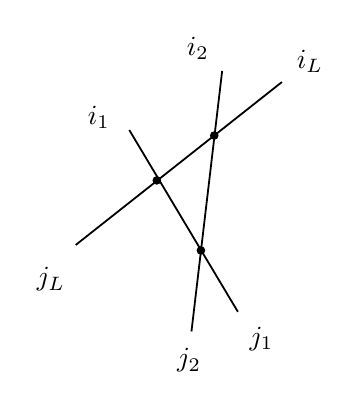
\begin{tikzpicture}[x=.01cm,y=-.01cm,line width=.65pt]
\draw (270,185)--(408,416) (388,110)--(349,441) (202,331)--(464,124);
\fill (305,249) circle[radius=.55mm];
\fill (378,192) circle[radius=.55mm];
\fill (361,338) circle[radius=.55mm];
\node[left] at (258,169) {\(i_1\)};
\node[above left] at (384,108) {\(i_2\)};
\node[above right] at (470,125) {\(i_L\)};
\node[below left] at (201,347) {\(j_L\)};
\node[below] at (346,450) {\(j_2\)};
\node[below right] at (410,423) {\(j_1\)};
\end{tikzpicture}}\endgroup}
\end{GelfandAdjacentEvidence}
\begin{GelfandAdjacentEvidence}{GELFAND-P000840}{2}


\uline{Associat.}: \(Z\) does not depend on the relative arrangement of the lines.

It suffices for it to hold for 3 lines:

\SourceFigure{GELFAND-P000840}{three-lines-equality}{%
\begingroup\color{black}\GelfandFitDiagram{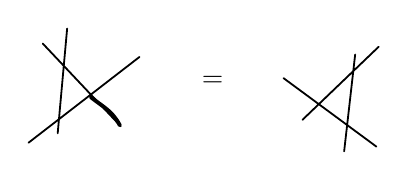
\begin{tikzpicture}[x=.010cm,y=-.010cm,line width=.65pt,line cap=round]
\draw (24,177)--(165,68) (42,51)--(141,156) (73,32)--(61,165);
\draw[line width=1.4pt] (103,119) .. controls (119,132) and (130,136) .. (140,155);
\node at (258,99) {\(=\)};
\draw (348,95)--(466,182) (372,148)--(469,55) (439,65)--(425,188);
\end{tikzpicture}}\endgroup\par
The thickened part of the descending line at left may be a retraced stroke or an arrow.}
\end{GelfandAdjacentEvidence}
\begin{GelfandAdjacentEvidence}{GELFAND-P000840}{3}


\uline{Prop. 2.} such matrices exist.

\uwave{On asymptotics}:

\begin{equation*}
\ln Z^{j_1\ldots j_L}_{i_1\ldots i_L}\sim L^2
\qquad\text{as }L\to\infty\tag{4}
\end{equation*}

(\uwave{if without associativity}) and the asympt. does not depend on the choice of indices \(i\) and \(j\).

[Under «asympt.»: (leading term)]

\uuline{Prop.} 3. Asymptotics as \(L\to\infty\)

\begin{equation*}
\ln Z(\lambda_1,\ldots,\lambda_L)
=\sum_{a>b=1}^{L}f(\lambda_a-\lambda_b)+\text{remainder term}\tag{5}
\end{equation*}
\Unclear{GELFAND-P000840}{asymptotic-index-limit}{The lower limit reads “\(a>b=1\).” The upper limit is \(L\).}
\end{GelfandAdjacentEvidence}
\begin{GelfandAdjacentEvidence}{GELFAND-P000840}{4}


(free en. of a large system \(=\) sum of pairwise

\uline{Opinion}: there are \(L\) kinds of particles; they move along straight lines and collide; on colliding they retain their velocities, but change \uuline{color}
\Unclear{GELFAND-P000840}{particle-model-heading}{The heading provisionally reads «Мнение» (“Opinion”).}
\end{GelfandAdjacentEvidence}
\begin{GelfandAdjacentEvidence}{GELFAND-P000840}{5}

\Unclear{GELFAND-P000840}{modified-velocity-word}{The opening strokes of the Russian word for “velocities” are overwritten. The earlier letterform is indistinguishable.}
\end{GelfandAdjacentEvidence}
\begin{GelfandAdjacentEvidence}{GELFAND-P000840}{6}


[Under «color»: (kind)]

Here \(Z\) — \(S\)-matrix;

There is an interpr. in which \(Z\) — the partition function

The weights of \(S\) — \(\exp\) of the potential. (probabilities?)

There are initial and \uwave{final colorings} \(i_1,\ldots,i_L\)
\[
j_1,\ldots,j_L.
\]

\SourceFigure{GELFAND-P000840}{particle-divider}{%
\begingroup\color{black}\GelfandFitDiagram{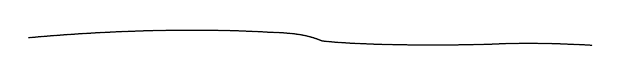
\begin{tikzpicture}[x=1cm,y=1cm,line width=.45pt]
\draw (0,0) .. controls (1.1,.10) and (2.2,.12) .. (3.06,.07)
 .. controls (3.41,.06) and (3.56,.03) .. (3.73,-.04)
 .. controls (4.13,-.09) and (5.23,-.11) .. (6.05,-.075)
 .. controls (6.48,-.063) and (6.83,-.079) .. (7.16,-.095);
\end{tikzpicture}}\endgroup}
\end{GelfandAdjacentEvidence}
\begin{GelfandAdjacentEvidence}{GELFAND-P000840}{7}


\uuline{A. Z.}

\SourceFigure{GELFAND-P000840}{spin-lines-diagram}{%
\begingroup\color{black}\GelfandFitDiagram{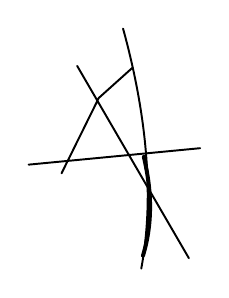
\begin{tikzpicture}[x=.011cm,y=-.011cm,line width=.7pt,line cap=round]
\draw (26,183)--(224,164) (82,69)--(211,291)
 (64,193)--(107,106)--(146,71);
\draw (135,26) .. controls (154,95) and (175,201) .. (156,303);
\draw[line width=1.45pt] (159,174) .. controls (165,200) and (172,242) .. (158,288);
\end{tikzpicture}}\endgroup\par
Two crossings near the horizontal line merge in a thickened stroke. The long divider is visible on the excerpt at left.}
\end{GelfandAdjacentEvidence}
\begin{GelfandAdjacentEvidence}{GELFAND-P000840}{8}


\uwave{spin} \uwave{variables} — in polygons; nearest-neighbor interaction;

\(S\) is chosen.
\Unclear{GELFAND-P000840}{s-expression-note}{The short note provisionally reads «подбирается» (“is chosen”). The opening letters and the heavy stroke remain unclear.}
\end{GelfandAdjacentEvidence}


\[
Z=\sum_{\{\sigma\}}e^{-\beta H}
\qquad H=\sum h(\sigma_A,\sigma_B)
\]

Exactly calculable partition functions — all of this kind!

\uline{For the Ising model}:
\[
S_{ij}^{k\ell}=\frac{ijk\ell+1}{2}e^{-\frac{\beta}{2}(i+j+k+\ell)}
\]

(after passing to the dual lattice)


\Needspace{7\baselineskip}
\begin{GelfandAdjacentEvidence}{GELFAND-P000841}{1}
\SourcePage{GELFAND-P000841}{unlabelled}
\uuline{24.9.79 }\qquad \uline{Gelfand Sem.}

\uwave{Renata Ernestovna KALLOSH} on the \uline{conf. in Cambridge}

(physicist)

(month-long working meeting on quantum grav., approx. 40 people)

20 people from the USA; including \uline{Chern, Singer, Milnor, Penrose};

Hawking, De Witt, Sciama, Coleman, Jackiw

[Below Hawking, with a short vertical stroke:] candidate for Newton’s vacant chair
\Unclear{GELFAND-P000841}{newton-abbreviation}{The abbreviation preceding “chair” is provisionally read «св.». The translation takes it as “vacant.”}
\end{GelfandAdjacentEvidence}
\begin{GelfandAdjacentEvidence}{GELFAND-P000841}{2}


\uline{Gibbons} — physicist, works with Hawking — talk on quantum grav.
\Unclear{GELFAND-P000841}{gibbons-abbreviation}{The abbreviation before “on quantum grav.” provisionally reads «докл.» (“talk”). «сем.» (“seminar”) is possible.}
\end{GelfandAdjacentEvidence}
\begin{GelfandAdjacentEvidence}{GELFAND-P000841}{3}


\uwave{Idea}: one must take account of the effects of nontriv. topology of space/time on small scales.

(many little “handles”).

The theory has yet to be constructed, but there has been signif. progress.

Mainly \uwave{Hawking}:
\Unclear{GELFAND-P000841}{hawking-coauth-abbreviation}{The Russian before Hawking provisionally reads «В основном» (“Mainly”). The opening strokes of the second word are faint.}
\end{GelfandAdjacentEvidence}
\begin{GelfandAdjacentEvidence}{GELFAND-P000841}{4}


1) \uwave{Space-time foam} (foam) — published in \uwave{Nuclear Physics}

(ordinary journ.)
\Unclear{GELFAND-P000841}{journal-gloss}{The note below the journal title is provisionally read «обычн. журн.» (“ordinary journ.”).}
\end{GelfandAdjacentEvidence}
\begin{GelfandAdjacentEvidence}{GELFAND-P000841}{5}


2) \uwave{Page, Atiyah} \quad something in the field of known gravitons
\Unclear{GELFAND-P000841}{page-atiyah-abbreviation}{The abbreviation provisionally reads «изв.» (“known”). «изл.» (“emitted”) is possible.}
\end{GelfandAdjacentEvidence}
\begin{GelfandAdjacentEvidence}{GELFAND-P000841}{6}


(from the group of Hawking)

3) \uwave{Coleman, Jackiw} \quad — on grav. taking topol. numbers into account —

on Yang–Mills.

(there is a survey on instanton methods)
\Unclear{GELFAND-P000841}{instanton-gloss}{The preposition before “methods” provisionally reads «о» (“on”). The letter is open and resembles «с».}
\end{GelfandAdjacentEvidence}
\begin{GelfandAdjacentEvidence}{GELFAND-P000841}{7}


4) \uwave{Milnor} — classif. of 4-dimensional manifolds

Someone on bundles on 4-manifolds.

5) \uwave{Singer} — on the signature of a 4-manifold.

\uwave{On supermanifolds}

Considered a route to quantization

De Witt is writing a book on supermanifolds

Singer is giving lectures
\SourceFigure{GELFAND-P000841}{ditto-stroke}{%
\begingroup\color{black}\GelfandFitDiagram{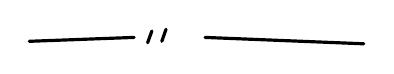
\begin{tikzpicture}[x=.9cm,y=.9cm,line width=1.15pt,line cap=round]
\draw (0,-.03)--(1.48,.025) (1.67,-.05)--(1.73,.115)
 (1.87,-.03)--(1.93,.14) (2.48,.025)--(4.72,-.065);
\end{tikzpicture}}\endgroup}
\end{GelfandAdjacentEvidence}
\begin{GelfandAdjacentEvidence}{GELFAND-P000841}{8}


\SourceFigure{GELFAND-P000841}{section-divider}{%
\begingroup\color{black}\GelfandFitDiagram{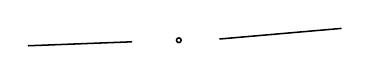
\begin{tikzpicture}[x=1cm,y=1cm,line width=.55pt,line cap=round]
\draw (0,-.06)--(1.31,-.01) (2.43,.026)--(3.97,.16);
\draw (1.91,.01) circle[radius=.03cm];
\end{tikzpicture}}\endgroup}
\end{GelfandAdjacentEvidence}
\begin{GelfandAdjacentEvidence}{GELFAND-P000841}{9}


\uwave{Something obtained independently by the speaker and by someone from the conf.}

[At right:] [Crossed out: \sout{Christen[…]}] Christensen, Duff;
\Unclear{GELFAND-P000841}{cancelled-author}{The crossed-out name provisionally reads “Christen[…].”}
\end{GelfandAdjacentEvidence}
\begin{GelfandAdjacentEvidence}{GELFAND-P000841}{10}


\uwave{Kallosh} — the speaker

Consider the eq.
\begin{equation*}
\Delta[A,B]\,\Phi[A,B]=0 \tag{1}
\end{equation*}

Here
\[
\phi[A,B]=\Psi_{\alpha_1\ldots\alpha_{2A},\,\dot\alpha_1,\ldots,\dot\alpha_{2B}}(x)
\]
— a multispinor, transforms under the group \(SO(4)\)
\Unclear{GELFAND-P000841}{group-symbol}{The second letter of the group name is open. It is provisionally set as \(SO(4)\).}
\end{GelfandAdjacentEvidence}
\begin{GelfandAdjacentEvidence}{GELFAND-P000841}{11}


\(x\in\) [Crossed out: \sout{…}] \(R^4\).
\Incomplete{GELFAND-P000841}{cancelled-space-symbol}{One sign is crossed out before \(R^4\). Its original form is indistinguishable.}
\end{GelfandAdjacentEvidence}
\begin{GelfandAdjacentEvidence}{GELFAND-P000841}{12}


\(\Delta\) — some operator; at one time from Hodge–de Rham.

there is also the half Dirac here
\Unclear{GELFAND-P000841}{operator-gloss}{The abbreviation before “Dirac” is provisionally read «пол.» and rendered “half.”}
\end{GelfandAdjacentEvidence}
\begin{GelfandAdjacentEvidence}{GELFAND-P000841}{13}


\[
S=A+B,\qquad T=A-B.
\]

\begin{equation*}
n[S;T]-n[s;T-1]=4^{s-1}\left[\left(T-\frac12\right)\chi+\left(s-\frac13\right)\frac12p\right]
\tag{2}
\end{equation*}
\Unclear{GELFAND-P000841}{formula-two-s-case}{The \(S/s\) forms in (2) vary in size. Their case is uncertain in places.}
\end{GelfandAdjacentEvidence}


[Below \(n\), with a short vertical stroke:] number of zero modes

(dim. of the solution space, with spin \(A\) and \(B\));

\(\chi,p\) — Euler and Pontryagin numbers


\Needspace{7\baselineskip}
\begin{GelfandAdjacentEvidence}{GELFAND-P000842}{1}
\SourcePage{GELFAND-P000842}{66}
Here there are the Gauss–Bonnet and Atiyah–Singer theorems, and so on.

\begin{equation*}
n[A,B]-2n\left[A\overset{?}{-}\frac12,B\right]
=4^{A+B-1}\left(A-\frac7{12}\right)\left(\chi+\frac12p\right).
\tag{3}
\end{equation*}
\Unclear{GELFAND-P000842}{formula-three-sign}{The sign before \(1/2\) is heavily inked over. A minus is a possible reading.}
\end{GelfandAdjacentEvidence}
\begin{GelfandAdjacentEvidence}{GELFAND-P000842}{2}


On nonzero modes:

\begin{equation*}
m[S;T]=m[S]=4^s m[0]
\tag{4}
\end{equation*}
\Unclear{GELFAND-P000842}{formula-four-s-case}{The case of \(s/S\) in the exponent is unclear. The last argument is provisionally set as \(0\).}
\end{GelfandAdjacentEvidence}
\begin{GelfandAdjacentEvidence}{GELFAND-P000842}{3}


[Under \(m[S;T]\):] nonzero modes:

\begin{equation*}
\Delta\Psi_i=\lambda_i\Psi_i
\tag{5}
\end{equation*}

In supergravity the nonzero modes cancel and only the contribution of the zero ones remains.

(3) [Crossed out: \sout{…}] only if the manifold is \uwave{self-dual}.
\Incomplete{GELFAND-P000842}{selfduality-cancellation}{The word is obscured by heavy crossing-out.}
\end{GelfandAdjacentEvidence}
\begin{GelfandAdjacentEvidence}{GELFAND-P000842}{4}


Hawking proved something earlier.

Coeff. in heat prop.
\Unclear{GELFAND-P000842}{heat-abbreviation}{The Russian abbreviation is provisionally read «теплопров.», rendered “heat prop.”}
\end{GelfandAdjacentEvidence}
\begin{GelfandAdjacentEvidence}{GELFAND-P000842}{5}


\[
B_4=n+m
\]

They proved that the funct. integral has no \uline{divergences}.

(in gravity)

The speaker did something too.

Interesting problem: the same on a supermanifold.

Singer is working on this now.

\SourceFigure{GELFAND-P000842}{separator-before-so}{%
\begingroup\color{black}\GelfandFitDiagram{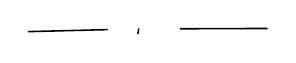
\begin{tikzpicture}[x=1cm,y=1cm,line width=.57pt,line cap=round]
\draw (0,0)--(1.00,.025) (1.39,-.025)--(1.40,.035) (1.93,.036)--(3.03,.04);
\end{tikzpicture}}\endgroup}
\end{GelfandAdjacentEvidence}
\begin{GelfandAdjacentEvidence}{GELFAND-P000842}{6}


The group \(SO(8)\), came up, something was wrong.

French group: [Crossed out: \sout{…}\,\((8)\)] symmetry \(E_7\) and
\Incomplete{GELFAND-P000842}{french-group-cancellation}{The crossed-out letters before the visible “(8)” cannot be read confidently.}
\end{GelfandAdjacentEvidence}
\begin{GelfandAdjacentEvidence}{GELFAND-P000842}{7}

\[
\underline{E_7\longrightarrow SU(8)}
\]

then \uwave{ext. supergravity}

\[
\dim E_7=133
\]

(\(E_7\) — comp. Lie group)
\Unclear{GELFAND-P000842}{exceptional-group-note}{The abbreviation before “Lie group” provisionally reads «комп.» (“comp.”).}
\end{GelfandAdjacentEvidence}
\begin{GelfandAdjacentEvidence}{GELFAND-P000842}{8}


\uwave{Interesting}

[Crossed out: \sout{…}] \uwave{to make a super index theorem}
\Incomplete{GELFAND-P000842}{index-theorem-cancelled-mark}{A mark before “to make” is inked out. Its original form is indistinguishable.}
\end{GelfandAdjacentEvidence}
\begin{GelfandAdjacentEvidence}{GELFAND-P000842}{9}


\uwave{Remarks}:

\(F_4\)

[Inserted above the line:] Hermitian

[Crossed out: \sout{…}] \uwave{matrices of order 3 made of octonions}; in them one constructs a Jordan add..
\Incomplete{GELFAND-P000842}{f4-cancellation}{A passage before “matrices” is crossed out. “Hermitian” is inserted above it.}
\end{GelfandAdjacentEvidence}
\begin{GelfandAdjacentEvidence}{GELFAND-P000842}{10}

\Unclear{GELFAND-P000842}{jordan-abbreviation}{The last abbreviation is provisionally read «слож.» (“add.”).}
\end{GelfandAdjacentEvidence}
\begin{GelfandAdjacentEvidence}{GELFAND-P000842}{11}


product \(\frac12(AB+BA)\).

one must take the automorphism group of this Jord. algebra. We get \(F_4\)

\uwave{Chern} — adviser to the Chin. president — works in \uwave{Chicago}.

\uwave{Yang} gives lectures in China to an audience of a thousand.

\uline{I. M. G.} — \uwave{what physicists said} about Einstein.

a) E. and N. Bohr are the greatest phys. of the century

b) E. did splendid work in his youth, but then spent 30–40 years on nonsense (tried to create a unified field theory).

c) \uwave{E. to Born}: “I want to invite you to Princeton, but an old nag, [Inserted above the line: like me,] no one takes seriously here.”
\Unclear{GELFAND-P000842}{einstein-quote-end}{The end of the quotation reads «никто не считается». An angled mark leads to the insertion “like me.”}
\end{GelfandAdjacentEvidence}
\begin{GelfandAdjacentEvidence}{GELFAND-P000842}{12}


[In the left margin:] \uuline{Blackboard}.
\Unclear{GELFAND-P000842}{margin-label}{The last letter of the Russian word is provisionally read «а».}
\end{GelfandAdjacentEvidence}
\begin{GelfandAdjacentEvidence}{GELFAND-P000842}{13}


\SourceFigure{GELFAND-P000842}{leaf-branch-diagram}{%
\begingroup\color{black}\GelfandFitDiagram{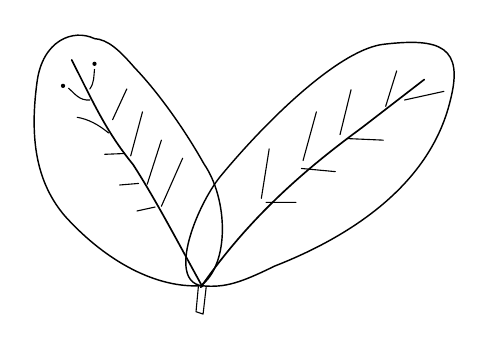
\begin{tikzpicture}[x=.010cm,y=-.010cm,line cap=round,line join=round]
\draw[line width=.52pt] (232,331) .. controls (178,334) and (114,303) .. (59,242)
 .. controls (27,204) and (13,153) .. (24,72)
 .. controls (31,19) and (70,4) .. (97,17)
 .. controls (114,18) and (129,32) .. (148,54)
 .. controls (175,82) and (209,128) .. (236,176)
 .. controls (267,221) and (269,304) .. (232,331);
\draw[line width=.52pt] (233,331) .. controls (189,324) and (227,229) .. (257,192)
 .. controls (319,117) and (411,29) .. (466,24)
 .. controls (536,16) and (567,27) .. (549,96)
 .. controls (522,208) and (413,272) .. (326,306)
 .. controls (283,327) and (263,334) .. (233,331);
\draw[semithick] (234,332) .. controls (202,274) and (175,222) .. (146,177)
 .. controls (111,134) and (95,97) .. (68,44);
\draw[semithick] (232,333) .. controls (297,239) and (373,177) .. (437,130)
 --(516,69);
\draw (91,81) .. controls (97,73) and (96,64) .. (97,56)
 (91,95) .. controls (78,96) and (72,87) .. (64,80)
 (115,137) .. controls (102,126) and (88,119) .. (75,117)
 (120,120)--(138,81)
 (143,166)--(158,110)
 (135,163)--(110,164)
 (164,202)--(182,146)
 (153,201)--(129,203)
 (182,230)--(209,169)
 (174,231)--(151,236);
\fill (97,49) circle[radius=2.7];
\fill (57,77) circle[radius=2.7];
\draw (309,220)--(319,157) (362,172)--(379,110)
 (409,139)--(423,82) (467,103)--(481,58)
 (315,225)--(353,225) (360,182)--(403,186)
 (418,144)--(464,146) (491,95)--(541,84);
\draw (229,332)--(226,364)--(235,367)--(239,332);
\end{tikzpicture}}\endgroup\par
The two outlines meet at the base. At right, some short branches are detached from the main line.}
\end{GelfandAdjacentEvidence}
\begin{GelfandAdjacentEvidence}{GELFAND-P000842}{14}


\uwave{connection of theor. physics with mathematics}:

in fundamental matters

(Yang’s drawing)

\SourceFigure{GELFAND-P000842}{lower-right-hatching}{%
\begingroup\color{black}\GelfandFitDiagram{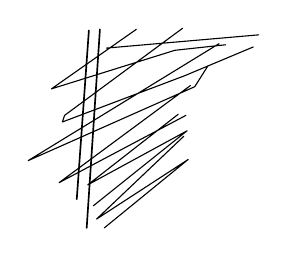
\begin{tikzpicture}[x=.014cm,y=-.014cm,line cap=round,line join=round]
\draw[semithick] (65,28)--(54,181) (75,27)--(63,207);
\draw (81,44)--(219,32)
 (108,27)--(31,81)--(143,46)--(189,41)
 (150,26)--(43,105)--(41,111)--(152,69)--(214,43)
 (183,40)--(10,146)--(161,79)--(173,60)
 (157,78)--(38,166)--(153,105)
 (146,104)--(64,168)--(154,119)--(69,187)
 (151,124)--(72,199)--(155,145)--(79,207);
\end{tikzpicture}}\endgroup\par
Near-vertical lines and diagonal hatching. The relationship to the drawing at left is unclear.}
\end{GelfandAdjacentEvidence}



\Needspace{7\baselineskip}
\begin{GelfandAdjacentEvidence}{GELFAND-P000843}{1}
\SourcePage{GELFAND-P000843}{unlabelled}
\uline{V. E. Zakharov.}

\SourceFigure{GELFAND-P000843}{reading-list-bracket}{%
\begingroup\color{black}\GelfandFitDiagram{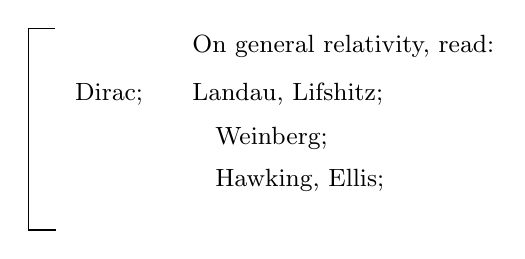
\begin{tikzpicture}[x=1cm,y=1cm,every node/.style={font=\small,inner sep=1pt}]
\draw[semithick] (.34,.35)--(0,.35)--(0,-2.21)--(.35,-2.21);
\node[anchor=west] at (2.04,.12) {\uline{On general relativity, read:}};
\node[anchor=west] at (.55,-.49) {Dirac;};
\node[anchor=west] at (2.04,-.49) {Landau, Lifshitz;};
\node[anchor=west] at (2.33,-1.05) {Weinberg;};
\node[anchor=west] at (2.33,-1.58) {Hawking, Ellis;};
\end{tikzpicture}}\endgroup\par
In the right margin. A left bracket groups the list.}
\end{GelfandAdjacentEvidence}
\begin{GelfandAdjacentEvidence}{GELFAND-P000843}{2}


\uwave{Mathematical problem}:

\[
k=(k_1,\ldots,k_N)
\]

Consider the fn. \(\omega(k)\) (real) and the space of pairs \((k_1,k_2)\) of dimension \(2N\) and there the eq.
\Unclear{GELFAND-P000843}{intro-short-word}{The short Russian word is provisionally read «там» (“there”).}
\end{GelfandAdjacentEvidence}
\begin{GelfandAdjacentEvidence}{GELFAND-P000843}{3}


\begin{equation*}
\omega(k_1+k_2)=\omega(k_1)+\omega(k_2)
\tag{1}
\end{equation*}

\(\omega\) — nonlin. \(\Rightarrow\) we get a surface \(\Gamma\) in \(R^{2n}\).

Is there another fn. \(f\), satisfying the same eq. on \(\Gamma\):
\[
f(k_1+k_2)=f(k_1)+f(k_2)
\]
and which does not differ from \(\omega\) by a linear one?
\Unclear{GELFAND-P000843}{linear-difference-verb}{The abbreviated verb after the negation is provisionally read «отлич.» (“differ”).}
\end{GelfandAdjacentEvidence}
\begin{GelfandAdjacentEvidence}{GELFAND-P000843}{4}


[Crossed out: \sout{This}]
\Unclear{GELFAND-P000843}{cancel-before-situation}{The crossed-out word provisionally reads «Это» (“This”).}
\end{GelfandAdjacentEvidence}
\begin{GelfandAdjacentEvidence}{GELFAND-P000843}{5}

This sit. is exceptional because the dimension is large.

Idea of Zakh. and Shulman:

how to get all eqs. having infinitely many first integrals.

\uline{Example}: \quad \uline{\(N=2\)}.

We will specify it by means of a parametrization, \(\vec{k}=(p,q)\);

[In small writing below the line:] implicitly \(\omega\) is given as follows:
\Unclear{GELFAND-P000843}{example-small-word}{The small Russian words provisionally read «в неявном виде» (“implicitly”).}
\end{GelfandAdjacentEvidence}
\begin{GelfandAdjacentEvidence}{GELFAND-P000843}{6}


\begin{equation*}
\omega(p,q),\qquad
\left[
\begin{aligned}
p&=\xi_1-\xi_2\\
q&=a(\xi_1)-a(\xi_2)\\
\omega&=b(\xi_1)-b(\xi_2)
\end{aligned}
\right.
\tag{2}
\end{equation*}

Another [Crossed out: \sout{…}] fn. \(f\):
\Incomplete{GELFAND-P000843}{cancelled-other-function}{A short entry before “fn.” is crossed out. The complete word is illegible.}
\end{GelfandAdjacentEvidence}
\begin{GelfandAdjacentEvidence}{GELFAND-P000843}{7}


\begin{equation*}
\left[
\begin{aligned}
p&=\xi_1-\xi_2\\
q&=a(\xi_1)-a(\xi_2)\\
f&=c(\xi_1)-c(\xi_2)
\end{aligned}
\right.
\qquad c\text{ — another fn. (arbitrary)}
\tag{3}
\end{equation*}
\Unclear{GELFAND-P000843}{third-system-rewritten}{Provisionally set as \(f=c(\xi_1)-c(\xi_2)\). The letter at left also resembles \(\varphi\), and the first at right resembles \(e\).}
\end{GelfandAdjacentEvidence}
\begin{GelfandAdjacentEvidence}{GELFAND-P000843}{8}


Question: is this a general construction?

Idea: we will give a parametrization of \(\Gamma\) (it is 3-dimensional)
\Unclear{GELFAND-P000843}{parametrization-pronoun}{The Russian endings provisionally read «она 3-мерна» (“it is 3-dimensional”).}
\end{GelfandAdjacentEvidence}
\begin{GelfandAdjacentEvidence}{GELFAND-P000843}{9}


\begin{equation*}
\begin{cases}
p_1=\xi_1-\xi_2\\
q_1=a(\xi_1)-a(\xi_2)\\
p_2=\xi_2-\xi_3\\
q_2=a(\xi_2)-a(\xi_3)
\end{cases}
\tag{4}
\end{equation*}

\[
\underbrace{p_1+p_2}_{p_3}\qquad
\underbrace{q_1+q_2}_{q_3}\qquad
p_3=\xi_1-\xi_3
\]

and so on.
\Unclear{GELFAND-P000843}{bottom-connector}{The opening sign is provisionally read «и» (“and”).}
\end{GelfandAdjacentEvidence}



\Needspace{7\baselineskip}
\begin{GelfandAdjacentEvidence}{GELFAND-P000844}{1}
\SourcePage{GELFAND-P000844}{67}
[Above the first line crossed out: \sout{…}]
\Incomplete{GELFAND-P000844}{top-cancelled}{A short entry above the first line is inked out. The letters are indistinguishable.}
\end{GelfandAdjacentEvidence}
\begin{GelfandAdjacentEvidence}{GELFAND-P000844}{2}


Hence if degenerate, then serious (functional parameter).
\Unclear{GELFAND-P000844}{opening-condition}{The short Russian word is provisionally read «если» (“if”).}
\end{GelfandAdjacentEvidence}
\begin{GelfandAdjacentEvidence}{GELFAND-P000844}{3}


There is a method of constr. systems with a Lax repr. (Zakharov–Shabat)
\begin{equation*}
\frac{\partial L}{\partial t}-\frac{\partial A}{\partial y}+[L,A]=0
\tag{5}
\end{equation*}

\[
\begin{aligned}
L&=\frac{\partial^n}{\partial x^n}+\ldots\\
A&=\frac{\partial^m}{\partial x^m}+\ldots
\end{aligned}
\]

(5) — nonlin. syst. of eqs. for the coeffs.

Consider its \uline{linearization}.
\SourceFigure{GELFAND-P000844}{linearization-connector}{%
\begingroup\color{black}\GelfandFitDiagram{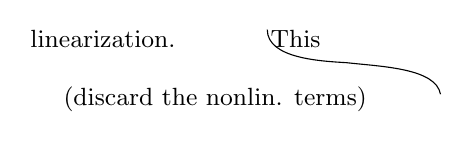
\begin{tikzpicture}[x=1cm,y=1cm,every node/.style={font=\small,inner sep=1pt}]
\node[anchor=west] at (0,0) {\uline{linearization}.};
\node[anchor=west] at (3.05,0) {This};
\node[anchor=west] at (.42,-.77) {(discard the nonlin. terms)};
\draw (3.05,.12) .. controls (3.05,-.25) and (3.74,-.28) .. (4.06,-.30)
 .. controls (4.51,-.35) and (5.19,-.37) .. (5.25,-.70);
\end{tikzpicture}}\endgroup\par
A note below the line. The connecting stroke reaches “This.”}
\end{GelfandAdjacentEvidence}
\begin{GelfandAdjacentEvidence}{GELFAND-P000844}{4}


This is a syst. with const. coeffs., it is solved by the method of Fourier.

\[
u_j\sim\exp(-\omega t+qy+px)
\]
\[
\omega=\omega(p,q)
\]

Those syst. look as in
\Unclear{GELFAND-P000844}{systems-phrase-start}{The opening Russian word provisionally reads «Те» (“Those”).}
\end{GelfandAdjacentEvidence}
\begin{GelfandAdjacentEvidence}{GELFAND-P000844}{5}

\Unclear{GELFAND-P000844}{systems-phrase-final}{After “as” there is a separate «в» (“in”). The sentence breaks off before the symbols.}
\end{GelfandAdjacentEvidence}
\begin{GelfandAdjacentEvidence}{GELFAND-P000844}{6}


\(a(\xi)\) — symbol of the oper. \(L\)

\(b(\xi)\) — ″ — \(A\)

[In the right margin:]
\SourceFigure{GELFAND-P000844}{side-note-separator}{%
\begingroup\color{black}\GelfandFitDiagram{\begin{tikzpicture}[x=1cm,y=1cm,every node/.style={inner sep=1pt}]
\draw (.22,.68)..controls (.25,.27) and (.17,-.19)..(.08,-.72);
\draw (.35,.66)..controls (.37,.25) and (.28,-.29)..(.23,-.81);
\node[anchor=west] at (.67,.19)
 {\(\begin{aligned}L&=L_0+\delta L\\ A&=A_0+\delta A\end{aligned}\)};
\end{tikzpicture}}\endgroup}
\end{GelfandAdjacentEvidence}
\begin{GelfandAdjacentEvidence}{GELFAND-P000844}{7}

\(\delta L,\delta A\) — everything that contains variable coeffs.

Degenerate disp. laws are connected with the inverse problem.

\[
\begin{aligned}
p&=\xi_1-\xi_2\\
q&=\ell(\xi_1)-\ell(\xi_2)\\
\omega&=a(\xi_1)-a(\xi_2)
\end{aligned}
\]
\(a,\ell\) — symbols of \(A_0,L_0\).

Consider the G.–L.–M. eq.:
\[
F+K+K\oplus F=0
\]
\Unclear{GELFAND-P000844}{circled-plus}{A circled plus is visible between \(K\) and \(F\).}
\end{GelfandAdjacentEvidence}
\begin{GelfandAdjacentEvidence}{GELFAND-P000844}{8}


\[
\begin{aligned}
\frac{\partial F}{\partial t}+[L_0,F]&=0\\
\frac{\partial F}{\partial y}+[A_0,F]&=0
\end{aligned}
\]
\Unclear{GELFAND-P000844}{retraced-derivative-plus}{The plus on the second line is retraced and still visible.}
\end{GelfandAdjacentEvidence}
\begin{GelfandAdjacentEvidence}{GELFAND-P000844}{9}


\[
K=-F
\]
\[
F=\exp\bigl(\xi_1x-\xi_2z+[\ell(\xi_1)-\ell(\xi_2)]y+[a(\xi_1)-a(\xi_2)]t\bigr)
\]
\Unclear{GELFAND-P000844}{exponential-overwritten-coordinate}{The letter after \(\xi_2\) is heavily overwritten. It provisionally reads \(z\).}
\end{GelfandAdjacentEvidence}
\begin{GelfandAdjacentEvidence}{GELFAND-P000844}{10}


Here the connection is estab. when \(\ell\) and \(a\) — polynomials. One can estab. a connection for rat. functions.
\Unclear{GELFAND-P000844}{retrace-ell}{The letter \(\ell\) before “and” has been retraced.}
\end{GelfandAdjacentEvidence}
\begin{GelfandAdjacentEvidence}{GELFAND-P000844}{11}


\SourceFigure{GELFAND-P000844}{polynomial-bracket}{%
\begingroup\color{black}\GelfandFitDiagram{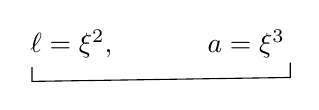
\begin{tikzpicture}[x=1cm,y=1cm,every node/.style={inner sep=1pt}]
\node at (.50,.25) {\(\ell=\xi^2,\)};
\node at (2.72,.25) {\(a=\xi^3\)};
\draw (0,-.04)--(0,-.22)--(3.28,-.17)--(3.28,.02);
\end{tikzpicture}}\endgroup}
\end{GelfandAdjacentEvidence}
\begin{GelfandAdjacentEvidence}{GELFAND-P000844}{12}


\(L,A\) are to be found — we get KdV.
\Unclear{GELFAND-P000844}{final-verb}{The Russian verb provisionally reads «ищутся» (“are to be found”).}
\end{GelfandAdjacentEvidence}



\Needspace{7\baselineskip}
\begin{GelfandAdjacentEvidence}{GELFAND-P000845}{1}
\SourcePage{GELFAND-P000845}{unlabelled}
Integr. by the inverse problem \(\Rightarrow\) the disp. law is degenerate.

\SourceFigure{GELFAND-P000845}{divider-first}{%
\begingroup\color{black}\GelfandFitDiagram{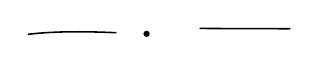
\begin{tikzpicture}[x=1cm,y=1cm,line width=.56pt,line cap=round]
\draw (0,-.02) .. controls (.36,.025) and (.82,.013) .. (1.11,0)
 (2.18,.054)--(3.32,.05);
\fill (1.50,-.014) circle[radius=.04cm];
\end{tikzpicture}}\endgroup}
\end{GelfandAdjacentEvidence}
\begin{GelfandAdjacentEvidence}{GELFAND-P000845}{2}


Matrices \(L\) and \(A\): no longer necessarily

[In the left margin:] \uline{Altern.}
\Unclear{GELFAND-P000845}{margin-alternative}{The underlined marginal word is provisionally read «Альтерн.» (“Altern.”).}
\end{GelfandAdjacentEvidence}
\begin{GelfandAdjacentEvidence}{GELFAND-P000845}{3}


If the eq. is integr. and the disp. law is nondeg., then the interaction \(\equiv 0\) on the manifold.
\Unclear{GELFAND-P000845}{resonance-abbreviation}{The final Russian abbreviation provisionally reads «мн-зии» (“manifold”).}
\end{GelfandAdjacentEvidence}
\begin{GelfandAdjacentEvidence}{GELFAND-P000845}{4}


\SourceFigure{GELFAND-P000845}{divider-second}{%
\begingroup\color{black}\GelfandFitDiagram{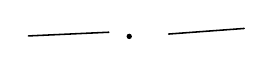
\begin{tikzpicture}[x=1cm,y=1cm,line width=.56pt,line cap=round]
\draw (0,-.04)--(1.02,.007) (1.78,-.016)--(2.74,.055);
\fill (1.28,-.046) circle[radius=.034cm];
\end{tikzpicture}}\endgroup}
\end{GelfandAdjacentEvidence}
\begin{GelfandAdjacentEvidence}{GELFAND-P000845}{5}


\[
\omega=\frac18\bigl[(p+\tfrac qp)^3-(-p+\tfrac qp)^3
=\frac14\bigl[p^3+\tfrac{3q^2}{p}\bigr]
\]
\Unclear{GELFAND-P000845}{dispersion-bracket}{No closing square bracket is visible before the second equals sign.}
\end{GelfandAdjacentEvidence}
\begin{GelfandAdjacentEvidence}{GELFAND-P000845}{6}


\uwave{Kad.–Petv. eq.}:
\[
u_t\overset{?}{+}\frac14
\left(u_{xxx}+6uu_x-3\int_{-\infty}^{x}u_{yy}\,dx\right)
\]
\Unclear{GELFAND-P000845}{kp-relation}{A vertical stroke crosses two horizontal strokes. A plus is provisional. The earlier sign is unclear.}
\end{GelfandAdjacentEvidence}
\begin{GelfandAdjacentEvidence}{GELFAND-P000845}{7}


I wrote out its symbol above.
\Unclear{GELFAND-P000845}{kp-note}{The Russian verb provisionally reads «выписал» (“I wrote out”). «выписан» (“is written out”) is possible.}
\end{GelfandAdjacentEvidence}
\begin{GelfandAdjacentEvidence}{GELFAND-P000845}{8}


\(\xi^2\) and \(\xi^3\) we dress — we get the K.–P. eq..

That is, K.–P. has exactly this disp. law (as in the example)

\SourceFigure{GELFAND-P000845}{divider-third}{%
\begingroup\color{black}\GelfandFitDiagram{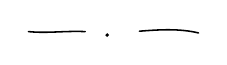
\begin{tikzpicture}[x=1cm,y=1cm,line width=.56pt,line cap=round]
\draw (0,0) .. controls (.24,-.024) and (.45,.011) .. (.72,0)
 (1.41,.005) .. controls (1.67,.026) and (1.92,.04) .. (2.16,-.017);
\fill (1.00,-.044) circle[radius=.025cm];
\end{tikzpicture}}\endgroup}
\end{GelfandAdjacentEvidence}
\begin{GelfandAdjacentEvidence}{GELFAND-P000845}{9}


\uwave{Experim. fact}: we dress a pair
\[
L_0=\begin{bmatrix}1&0\\0&-1\end{bmatrix}\frac{\partial}{\partial x},
\qquad
A_0=\begin{bmatrix}1&0\\0&1\end{bmatrix}\frac{\partial^2}{\partial x^2}
\]
We get
\[
L=\begin{bmatrix}1&0\\0&-1\end{bmatrix}\frac{\partial}{\partial x}
+\begin{bmatrix}0&\psi\\\bar\psi&0\end{bmatrix}
\]
and the eq.
\begin{equation*}
\left\{\begin{aligned}
i\frac{\partial\psi}{\partial t}-\frac{\partial^2\psi}{\partial x^2}
+\frac{\partial^2\psi}{\partial y^2}+u\psi&=0\\
\left(\frac{\partial^2}{\partial x^2}+\frac{\partial^2}{\partial y^2}\right)u
&=\left(\frac{\partial^2}{\partial x^2}-\frac{\partial^2}{\partial y^2}\right)|\psi|^2
\end{aligned}\right.
\tag{6}
\end{equation*}
D…–Stewartson syst. (see hydrodyn., theory of surface waves)
\Unclear{GELFAND-P000845}{system-name}{The first name begins with the Russian «Д» (“D”). Its continuation is indistinct.}
\end{GelfandAdjacentEvidence}
\begin{GelfandAdjacentEvidence}{GELFAND-P000845}{10}


Take the Fourier trans. We get a syst. of the form:
\[
\psi\to a(k)
\]
\[
i\frac{\partial a(k)}{\partial t}=\frac{\delta H}{\delta a(k)}
\]
\Unclear{GELFAND-P000845}{variational-denominator}{There is no visible bar over \(a(k)\) in the denominator of the variational derivative.}
\end{GelfandAdjacentEvidence}
\begin{GelfandAdjacentEvidence}{GELFAND-P000845}{11}


\[
\begin{aligned}
H={}&\int\omega_k|a_k|^2\,dk\\
&+\int w^{[\Gamma]}_{kk_1k_2k_3}
\bar a_k\bar a_{k_1}a_{k_2}a_{k_3}
\delta_{k+k_1-k_2-k_3}\,dk_2\,dk_3
\end{aligned}
\]
\Unclear{GELFAND-P000845}{hamiltonian-coefficient}{The coefficient is provisionally read \(w\). A separate mark at upper right resembles \(\Gamma\).}
\end{GelfandAdjacentEvidence}
\begin{GelfandAdjacentEvidence}{GELFAND-P000845}{12}

\Unclear{GELFAND-P000845}{hamiltonian-measure}{Two differentials are visible at the frame edge. The first subscript is provisionally read as \(2\).}
\end{GelfandAdjacentEvidence}
\begin{GelfandAdjacentEvidence}{GELFAND-P000845}{13}


\[
w=\frac{(p_1-p_3)^2-(q_1-q_3)^2}{(p_1-p_3)^2+(q_1-q_3)^2}
+\frac{(p_2-p_4)^2-(q_2-q_4)^2}{(p_2+p_4)^2+(q_2+q_4)^2}
\]
\Unclear{GELFAND-P000845}{bottom-first-q}{The subscript on the first \(q\) on both lines of the first fraction is provisionally read as \(1\).}
\end{GelfandAdjacentEvidence}
\begin{GelfandAdjacentEvidence}{GELFAND-P000845}{14}

\Unclear{GELFAND-P000845}{bottom-denominator-signs}{Plus signs are visible inside both parentheses of the second denominator.}
\end{GelfandAdjacentEvidence}



\Needspace{7\baselineskip}
\begin{GelfandAdjacentEvidence}{GELFAND-P000846}{1}
\SourcePage{GELFAND-P000846}{68}
In the space of \(k_1,k_2,k_3,k_4\)
\Unclear{GELFAND-P000846}{fourth-wave-vector}{The letter with subscript \(4\) is retraced. It is provisionally set as \(k_4\).}
\end{GelfandAdjacentEvidence}
\begin{GelfandAdjacentEvidence}{GELFAND-P000846}{2}


consider the eq.
\[
\begin{gathered}
\omega(k_1)+\omega(k_2)=\omega(k_3)+\omega(k_4);\\
k_1+k_2=k_3+k_4
\end{gathered}
\]
[Crossed out: \sout{…}]
\Incomplete{GELFAND-P000846}{cancelled-top-line}{A short entry and a long line below the equations are heavily crossed out. The text is illegible.}
\end{GelfandAdjacentEvidence}
\begin{GelfandAdjacentEvidence}{GELFAND-P000846}{3}


It turns out that \(w|_\Gamma=0\).

\uline{Arnold’s conj.}: This is Poincaré’s theor. \uwave{on integrability}. (when there is a first int. indep. of the en.)

Poincaré’s cond.: the ampl. of reson. harmonics must be \(0\)

(see Poincaré, cel. mech., or Arnold: suppl. chapters)

\uwave{Poincaré}: Hamiltonian
\[
H=H_0(p)+\varepsilon\sum h_k(p)e^{ikq}
\]

\(p=I,\quad q=\psi\).
\Unclear{GELFAND-P000846}{angle-symbol}{The angle sign is provisionally read \(\psi\). \(\varphi\) is possible.}
\end{GelfandAdjacentEvidence}
\begin{GelfandAdjacentEvidence}{GELFAND-P000846}{4}


When \(\exists\) an int. \(F(p,q,\varepsilon)\) (everything is periodic in \(q\)),

[Under \(F\):] indep. of \(H\).

\uwave{Nec. condition}: form \(\lambda=\frac{\partial H_0}{\partial p}\) and impose a nondeg. condition on it.
\Unclear{GELFAND-P000846}{nondegeneracy-lambda}{The sign to the left of the derivative is heavily retraced. It is provisionally set as \(\lambda\).}
\end{GelfandAdjacentEvidence}
\begin{GelfandAdjacentEvidence}{GELFAND-P000846}{5}


\[
\det\left|\frac{\partial\lambda}{\partial p}\right|\ne0
\]
\Unclear{GELFAND-P000846}{determinant-lambda}{The sign in the numerator is also retraced. It is provisionally set as \(\lambda\).}
\end{GelfandAdjacentEvidence}
\begin{GelfandAdjacentEvidence}{GELFAND-P000846}{6}

— one of the nondeg. conditions. (there are 2 in all)

There are no integrals if
\[
\Gamma:\quad\langle k,\lambda(p)\rangle=0
\]
\Unclear{GELFAND-P000846}{resonance-lambda}{The sign before \((p)\) is retraced. It is provisionally set as \(\lambda\).}
\end{GelfandAdjacentEvidence}
\begin{GelfandAdjacentEvidence}{GELFAND-P000846}{7}


Poincaré’s cond.:
\[
\underline{h_k|_{\Gamma_k}=0},\qquad k\in\mathbb Z^n.
\]
if it is violated infinitely often, there is no integral

Idea: \(\lambda\leftrightarrow\omega\).

\uline{Arn.} \quad formulas (2) mean there is a \uwave{transl. surface}.

\SourceFigure{GELFAND-P000846}{diagram-01}{%
\begingroup\color{black}\GelfandFitDiagram{\begin{tikzpicture}[x=.013cm,y=-.013cm,line cap=round,line width=.60pt]
\draw (11,163) .. controls (44,156) and (99,128) .. (135,89)
 .. controls (149,73) and (166,43) .. (171,26);
\draw[semithick] (60,145) .. controls (79,158) and (99,210) .. (102,262);
\draw[semithick] (58,154) .. controls (48,148) and (57,129) .. (65,134)
 .. controls (74,140) and (66,153) .. (58,154);
\end{tikzpicture}}\endgroup\par
The curves meet near a small loop. The thickening at left and the loop are drawn as visible. No arrows can be distinguished confidently.}
\end{GelfandAdjacentEvidence}
\begin{GelfandAdjacentEvidence}{GELFAND-P000846}{8}


we move the 2nd curve along the 1st,

translating it in parallel

\uline{Curves}:
\[
\begin{aligned}
p&=\xi_1; &\qquad p&=-\xi_2\\
q&=a(\xi_1); &q&=-a(\xi_2)\\
\omega&=b(\xi_1); &\omega&=-b(\xi_2)
\end{aligned}
\]

The curve moves by itself.

\uuline{Zakharov}.
\[
\omega_1(k_1+k_2)=\omega_2(k_1)+\omega_3(k_2)
\]
we get general transl. surfaces.

\SourceFigure{GELFAND-P000846}{transfer-divider}{%
\begingroup\color{black}\GelfandFitDiagram{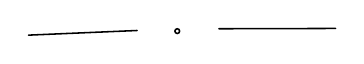
\begin{tikzpicture}[x=1cm,y=1cm,line cap=round,line width=.56pt]
\draw (0,0)--(1.38,.059) (2.42,.081)--(3.90,.085);
\draw (1.89,.051) circle[radius=.030cm];
\end{tikzpicture}}\endgroup}
\end{GelfandAdjacentEvidence}
\begin{GelfandAdjacentEvidence}{GELFAND-P000846}{9}


\uwave{Procedure}. We check whether the disp. law is degen., then see.

\(0\) or not \(0\) there, the Ham. interaction.
\Unclear{GELFAND-P000846}{final-coefficient}{The abbreviation before “interaction” provisionally reads «гам.» (“Ham.”).}
\end{GelfandAdjacentEvidence}


What if the integrals start directly at higher orders?


\Needspace{7\baselineskip}
\begin{GelfandAdjacentEvidence}{GELFAND-P000847}{1}
\SourcePage{GELFAND-P000847}{unlabelled}
\uuline{Arn.} \quad \uwave{Birkhoff}.
\Unclear{GELFAND-P000847}{first-birkhoff}{The opening abbreviation reads «Арн.» (“Arn.”). The full stop after the following word is unclear.}
\end{GelfandAdjacentEvidence}
\begin{GelfandAdjacentEvidence}{GELFAND-P000847}{2}


\[
H=\sum\omega_k z_k\bar z_k+\ldots
\]

[crossed out: \sout{\(H=\)}]
\Unclear{GELFAND-P000847}{cancelled-h}{\(H\) can be read under the strokes. An equals sign may follow it.}
\end{GelfandAdjacentEvidence}
\begin{GelfandAdjacentEvidence}{GELFAND-P000847}{3}

\[
\sum\omega_k(p_k^2+q_k^2)+\ldots
\]

[At right:]
\[
z=p+iq,\qquad \Pi_k=z_k\bar z_k
\]

Birkhoff: \uwave{in the nonres. case, red. to \(H(\Pi_k)\)}.
\Unclear{GELFAND-P000847}{nonresonant-abbreviation}{The abbreviation after “case” is provisionally read «прив.» (“red.”).}
\end{GelfandAdjacentEvidence}
\begin{GelfandAdjacentEvidence}{GELFAND-P000847}{4}


(if the \(\omega_k\) are independent)

[At right:] (at the level of form. series)

\uline{I. M. G.} \quad \uwave{Short list of what one needs to know}.

1. \uwave{Modern abstr. language} \quad (see e.g. the 1st part of the book by \uline{Kirillov})
\SourceFigure{GELFAND-P000847}{glossary-arrow}{%
\begingroup\color{black}\GelfandFitDiagram{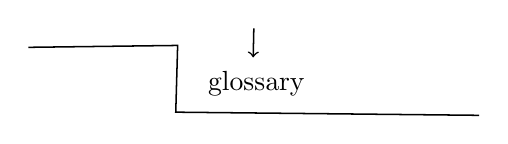
\begin{tikzpicture}[x=.008cm,y=-.008cm,line width=.55pt,every node/.style={inner sep=1pt}]
\draw (31,47)--(268,44)--(265,150)--(747,155);
\draw[->] (389,17)--(388,63);
\node at (393,105) {\uwave{glossary}};
\end{tikzpicture}}\endgroup\par
A stepped stroke and an arrow pointing to “glossary” are below the reference.}
\end{GelfandAdjacentEvidence}
\begin{GelfandAdjacentEvidence}{GELFAND-P000847}{5}


2. \uline{Arnold}: diff. eqs. \(+\) suppl. chapters

(to get used to analysis)

3. \uwave{On algebra}: 2 chapters of the book by \uline{Serre} on
[crossed out: \sout{representations}] reprs. of finite groups.
\Unclear{GELFAND-P000847}{algebra-cancelled}{The crossed-out word provisionally reads «представлениям» (“representations”).}
\end{GelfandAdjacentEvidence}
\begin{GelfandAdjacentEvidence}{GELFAND-P000847}{6}


[Above the line crossed out: \sout{all}]
\Unclear{GELFAND-P000847}{all-cancelled}{The crossed-out word provisionally reads «все» (“all”).}
\end{GelfandAdjacentEvidence}
\begin{GelfandAdjacentEvidence}{GELFAND-P000847}{7}


all except \uwave{ch. 1} of the book by \uline{Serre} on Lie grps. and algebras
(especially the last chapter)

[Above the line crossed out: \sout{…}]
\Incomplete{GELFAND-P000847}{linear-cancelled}{A short word above “Lin. algebra” is crossed out. It is illegible.}
\end{GelfandAdjacentEvidence}
\begin{GelfandAdjacentEvidence}{GELFAND-P000847}{8}


\uwave{Lin. algebra}: Gelfand; Maltsev

4. \uwave{Diff. geometry} in 2 vers.: the old tensor version
(see \uline{Dirac} on the theory of rel.; and \uline{Landau and Lifshitz})
\Unclear{GELFAND-P000847}{old-tensor-otn}{The abbreviation after “theory” provisionally reads «отн.» (“rel.”).}
\end{GelfandAdjacentEvidence}


modern vers.: vector bundles and connections.

5. \uwave{Representations}: H. Weyl

lectures of Raka \quad Racah.

Gelfand, Minlos, Shapiro


\clearpage
\pdfbookmark[0]{Chapter 16}{gelfand-archive-chapter-16}
\section*{Chapter 16}


\Needspace{7\baselineskip}
\begin{GelfandAdjacentEvidence}{GELFAND-P000848}{1}
\SourcePage{GELFAND-P000848}{1}
\uline{1.10.79} \qquad \uline{Gelfand Sem.}
\Unclear{GELFAND-P000848}{date-header}{The month is provisionally read as “10.” The second digit is incomplete in the scan.}
\end{GelfandAdjacentEvidence}
\begin{GelfandAdjacentEvidence}{GELFAND-P000848}{2}


[Crossed-out heading: \sout{KALLOSH?}]
\Unclear{GELFAND-P000848}{top-cancelled-heading}{«КАЛЛОШ» (“KALLOSH”) is a possible reading of the crossed-out heading.}
\end{GelfandAdjacentEvidence}
\begin{GelfandAdjacentEvidence}{GELFAND-P000848}{3}


\uline{I. M. G.} What is a spinor?

\uwave{Pauli’s book on quant. mech.} — the best expos. of Dirac’s theory (Dirac eq.)
\Unclear{GELFAND-P000848}{book-abbreviation}{The overwritten abbreviation is provisionally read «квант.» (“quant.”).}
\end{GelfandAdjacentEvidence}
\begin{GelfandAdjacentEvidence}{GELFAND-P000848}{4}


His objections to Dirac’s theor.:

a) exist. of \uline{positrons}, predicted by Dirac’s theor.

b) if they exist, then on colliding with a positr. one gets 2 photons
\Unclear{GELFAND-P000848}{annihilation-word}{The abbreviation after “with” is provisionally read «позитр.» (“positr.”).}
\end{GelfandAdjacentEvidence}
\begin{GelfandAdjacentEvidence}{GELFAND-P000848}{5}


c) according to this theory 2 photons can produce an electr./positron pair
\Unclear{GELFAND-P000848}{pair-abbreviation}{The abbreviation before the slash is tentatively read «эл-н» (“electr.”).}
\end{GelfandAdjacentEvidence}
\begin{GelfandAdjacentEvidence}{GELFAND-P000848}{6}


Dirac refus., so that they would not make him “Sir” (?)
\Unclear{GELFAND-P000848}{dirac-abbreviation}{The abbreviation after “Dirac” is provisionally read «отказ.» (“refus.”).}
\end{GelfandAdjacentEvidence}
\begin{GelfandAdjacentEvidence}{GELFAND-P000848}{7}


[The lines are grouped by a bracket on the left.]

Once someone told him that he did not understand the form. in the lower left corner of the board.

Dirac does not answer.

The chairman asks him to answer

[Crossed out: \sout{…}] Dirac: “there was no question, there was a statement.”
\Incomplete{GELFAND-P000848}{anecdote-cancelled-word}{The crossed-out fragment before “Dirac” is illegible.}
\end{GelfandAdjacentEvidence}
\begin{GelfandAdjacentEvidence}{GELFAND-P000848}{8}

\SourceFigure{GELFAND-P000848}{anecdote-bracket}{%
\begingroup\color{black}\GelfandFitDiagram{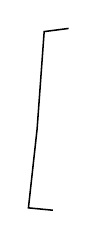
\begin{tikzpicture}[x=.01cm,y=-.01cm,line width=.55pt]
\draw (69,16)--(38,20)--(29,144)--(18,244)--(49,247);
\end{tikzpicture}}\endgroup\par
Bracket to the left of the preceding four lines.}
\end{GelfandAdjacentEvidence}
\begin{GelfandAdjacentEvidence}{GELFAND-P000848}{9}


\uwave{Hamilton}: wanted to extract the root of \(x^2+y^2+z^2\), and obtain a “lin. form”
\[
-(x^2+y^2+z^2)=(ax+by+cz)^2
\]
\[
a^2=b^2=c^2=-1
\]
\Unclear{GELFAND-P000848}{hamilton-square-sign}{The overwritten sign after \(c^2\) is provisionally read \(=-1\).}
\end{GelfandAdjacentEvidence}
\begin{GelfandAdjacentEvidence}{GELFAND-P000848}{10}

\[
\begin{aligned}
&(ab+ba)\,[?]\,xy+(ac+ca)xz+(bc+cb)yz\\
&\qquad{}+a^2x^2+b^2y^2+c^2z^2=-(x^2+y^2+z^2).
\end{aligned}
\]
\Unclear{GELFAND-P000848}{hamilton-factor-mark}{There is an unresolved dark stroke between the first parenthesis and \(xy\).}
\end{GelfandAdjacentEvidence}
\begin{GelfandAdjacentEvidence}{GELFAND-P000848}{11}


hence the relations
\[
ab+ba=0 \quad \text{etc.}
\]
Add the unit — get \uwave{quaternions}.

Consider the transformation
\[
z'=\frac{az+b}{cz+d}
\]

or
\[
\begin{cases}
z'_1=az_1+bz_2\\
z'_2=cz_1+dz_2
\end{cases}
\qquad z'=\frac{z'_1}{z'_2},\quad z=\frac{z_1}{z_2}.
\]

Spinors — a pair of numbers [below “numbers”: (compl.)], transf. according to this law

Compl. conj. — \uline{conj.} \uline{spinor}.
\SourceFigure{GELFAND-P000848}{spinor-divider}{%
\begingroup\color{black}\GelfandFitDiagram{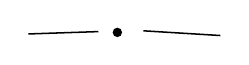
\begin{tikzpicture}[x=.01cm,y=-.01cm,line width=.55pt]
\draw (19,47)--(108,44);
\fill (132,45) circle[radius=1.7pt];
\draw (165,43)--(263,49);
\end{tikzpicture}}\endgroup\par
Two short strokes with a dot between them.}
\end{GelfandAdjacentEvidence}
\begin{GelfandAdjacentEvidence}{GELFAND-P000848}{12}


\uline{Gravitation} should be read in Landau and Lifshitz (vol. 2)

\uwave{chs. 1, 2, 10, 11.}

\uwave{Renata E. Kallosh.}

\uline{Program.}

1. Two-component spinors.

2. Self-duality.

3. Diff. operator \(\Delta(A,B)\), descr. the eq. for particles of higher spins.

4. Heat eq., zero and nonzero modes.

5. Index theorems.

6. Supertheor. in a grav. field

7. Superself-duality.

(8. Index supertheor.! Singer is working on it, but in fact there is no such theorem)
\Unclear{GELFAND-P000848}{program-last-number}{The numeral after the opening parenthesis is tentatively read as 8.}
\end{GelfandAdjacentEvidence}
\begin{GelfandAdjacentEvidence}{GELFAND-P000848}{13}

\Unclear{GELFAND-P000848}{program-last-verb}{The opening phrase is provisionally read «Ею занимается» (“is working on it”).}
\end{GelfandAdjacentEvidence}



\Needspace{7\baselineskip}
\begin{GelfandAdjacentEvidence}{GELFAND-P000849}{1}
\SourcePage{GELFAND-P000849}{unlabelled}
\uline{Refs.}

1. [Crossed out: \sout{…}] \uline{S. W. Hawking}, \uline{C. N. Pope}
\Incomplete{GELFAND-P000849}{bibliography-first-cancelled}{A short fragment before “S. W. Hawking” is crossed out and illegible.}
\end{GelfandAdjacentEvidence}
\begin{GelfandAdjacentEvidence}{GELFAND-P000849}{2}


Nucl. Phys., B 146 (1978), 381
\Unclear{GELFAND-P000849}{bibliography-first-year}{The final digit of the year is provisionally read as 8. The strokes could also be read as 1.}
\end{GelfandAdjacentEvidence}
\begin{GelfandAdjacentEvidence}{GELFAND-P000849}{3}


2. \uline{R. E. Kallosh}, JETP Letters,

\uline{29} (1979), 192; 493

3. S. M. Christensen, M. J. Duff.

Nucl. Phys. (1979), 301

4. — „ —, — „ — Deser, Gr[?]
\Unclear{GELFAND-P000849}{bibliography-fourth-last-author}{The name after “Deser” is provisionally read “Gr” with an unclear ending. The first letter could be read as “C.”}
\end{GelfandAdjacentEvidence}
\begin{GelfandAdjacentEvidence}{GELFAND-P000849}{4}


Phys Lett. \uline{84 B} (1979), 411

[1] — main contrib. in supergrav. (in the 1-loop approx.) — from \(0^{\underline{\text{х}}}\) modes
\Unclear{GELFAND-P000849}{superscript-zero}{There is a small underlined superscript «х» (the Russian ordinal ending) at the zero.}
\end{GelfandAdjacentEvidence}
\begin{GelfandAdjacentEvidence}{GELFAND-P000849}{5}


(in Y.-M. — from all modes!)

[2], [3] indep. — in supergrav. (for self-dual) for higher orders

Before this it was so in the 1st and 2nd ord. supergrav. did not cont. diverg.
\Unclear{GELFAND-P000849}{before-supergravity}{The word after “Before this” is provisionally read «было» (“it was”). The last letter is unclear.}
\end{GelfandAdjacentEvidence}
\begin{GelfandAdjacentEvidence}{GELFAND-P000849}{6}


[3] based on the ordinary index theor.

\uwave{Two-comp. van der Waerden formalism.}

\[
\Psi_\alpha\longrightarrow\Psi_\beta\Omega_\alpha^\beta \tag{1}
\]

[At right:] Transformation law

\(\Psi_\alpha\in(\text{repr. stand. 2-dim. repr. }SL(2,C))=V;\)
\Unclear{GELFAND-P000849}{margin-representation-abbreviation}{The first abbreviation is provisionally read «пр.» (“repr.”). Its initial letter could be «и».}
\end{GelfandAdjacentEvidence}
\begin{GelfandAdjacentEvidence}{GELFAND-P000849}{7}


\(\Psi_{\dot\alpha}\in\bar V\), \(V\otimes\bar V\) has a real str.
and the gr. \(SL(2,C)\) pres. the quad. form.

(gr. e.g. in Penrose)
\Unclear{GELFAND-P000849}{preserve-quadratic-form}{The abbreviation in parentheses is provisionally read «напр.» (“e.g.”).}
\end{GelfandAdjacentEvidence}
\begin{GelfandAdjacentEvidence}{GELFAND-P000849}{8}


\(SL(2,C)\) as a real Lie man.
\Unclear{GELFAND-P000849}{margin-real-lie}{The abbreviation after “real” is provisionally read «мн.» (“man.”). «гр.» (“gr.”) is possible.}
\end{GelfandAdjacentEvidence}
\begin{GelfandAdjacentEvidence}{GELFAND-P000849}{9}

\SourceFigure{GELFAND-P000849}{margin-stepped-bracket}{%
\begingroup\color{black}\GelfandFitDiagram{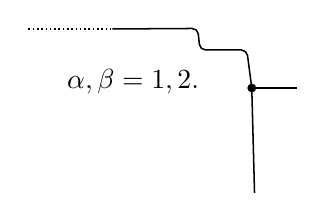
\begin{tikzpicture}[x=.007cm,y=-.007cm,line width=.55pt,every node/.style={inner sep=0pt}]
\draw[densely dotted] (15,32)--(167,32);
\draw[rounded corners=2pt] (167,32)--(322,31)--(326,70)--(411,70)--(420,139);
\draw (420,139)--(425,329);
\draw (420,139)--(502,139);
\fill (420,139) circle[radius=1.6pt];
\node[anchor=west] at (84,128) {\(\alpha,\beta=1,2.\)};
\end{tikzpicture}}\endgroup\par
A stepped line between the index formula and the note at right. A short line extends right from the dot. The correspondence between strokes and lines of text is unclear.}
\end{GelfandAdjacentEvidence}
\begin{GelfandAdjacentEvidence}{GELFAND-P000849}{10}


[Main text:] If the Lorentz gr. or \(SO(4)\)
\[
\Omega_\alpha^\beta=(\omega^{ab}\Sigma_{ab})_\alpha^\beta \tag{2}
\]
\(\alpha,\beta=1,2.\)

(transf. law of a two-comp. spinor)

\(\Sigma_{ab}\) — fixed matrices (like the Pauli matr.) of order 2

\(\omega^{ab}\) — parameters

For the Pauli matrices
\[
\sigma_i\sigma_j=\delta_{ij}+\epsilon_{ijk}\sigma^k \tag{3}
\]
\Unclear{GELFAND-P000849}{pauli-product-source}{The letter \(\epsilon\) is visible after the plus sign in (3). No separate factor precedes it.}
\end{GelfandAdjacentEvidence}
\begin{GelfandAdjacentEvidence}{GELFAND-P000849}{11}

\[
\sigma^a=(I,i\vec\sigma),\qquad a=1,2,3,4.
\]
\[
\Sigma_{ab}=\sigma_a\bar\sigma_b-\bar\sigma_b\sigma_a \tag{4}
\]

Now about quantities in spinor notation.

\uwave{Penrose} formulated the theory of gravitation in this way.

Let there be a vector \(x_a\); then
\[
X_{\alpha\dot\alpha}=\sigma^a_{\alpha\dot\alpha}x_a\quad\text{— spinor} \tag{5}
\]
\[
\Psi_{\alpha_1\ldots\alpha_{2A},\dot\alpha_1\ldots\dot\alpha_{2B}}=\Psi(A,B) \tag{6}
\]
\Unclear{GELFAND-P000849}{equation-six-first-dotted-index}{The first dotted index is provisionally set as \(\dot\alpha_1\). The numeral can also be read as 2.}
\end{GelfandAdjacentEvidence}



\Needspace{7\baselineskip}
\begin{GelfandAdjacentEvidence}{GELFAND-P000850}{1}
\SourcePage{GELFAND-P000850}{2}
and if one fully symmetrizes, one gets an irred. representation.

Incidentally, about the Pauli matrices: they are as follows.
\[
\left\{\begin{aligned}
\sigma^1_{\alpha\dot\alpha}&=\frac{1}{\sqrt2}\begin{pmatrix}0&1\\1&0\end{pmatrix};\\
\sigma^2_{\alpha\dot\alpha}&=\frac{1}{\sqrt2}\begin{pmatrix}0&-i\\i&0\end{pmatrix};\\
\sigma^3_{\alpha\dot\alpha}&=\frac{1}{\sqrt2}\begin{pmatrix}1&0\\0&-1\end{pmatrix};\\
\sigma^4_{\alpha\dot\alpha}&=\frac{1}{\sqrt2}\begin{pmatrix}1&0\\0&1\end{pmatrix}.
\end{aligned}\right. \tag{7}
\]
\Unclear{GELFAND-P000850}{pauli-first-index-overwritten}{The first lower index of \(\sigma^1\) is overwritten. The upper layer reads \(\alpha\). The earlier sign is illegible.}
\end{GelfandAdjacentEvidence}
\begin{GelfandAdjacentEvidence}{GELFAND-P000850}{2}


There is also \(\epsilon^{\alpha\beta}\)
\[
\epsilon^{12}=1,\qquad\epsilon_{\alpha\beta}=\begin{bmatrix}0&1\\-1&0\end{bmatrix} \tag{8}
\]

Lowering indices:
\[
\Psi_\alpha=\epsilon_{\alpha\beta}\Psi^\beta \tag{9}
\]

\uline{I. M. G.}

In coord. \(\dot\alpha\) the transf. is complex conjugate.

Form. (5) — \uwave{constr. of a spinor from a vector}
\SourceFigure{GELFAND-P000850}{circled-emphasis}{%
\begingroup\color{black}\GelfandFitDiagram{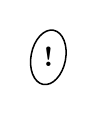
\begin{tikzpicture}[line width=.55pt]
\draw[rotate=-11] (0,0) ellipse[x radius=.22cm,y radius=.35cm];
\node[font=\bfseries] at (0,0) {!};
\end{tikzpicture}}\endgroup\par
Circled exclamation mark to the left of the line about formula (5).}
\end{GelfandAdjacentEvidence}
\begin{GelfandAdjacentEvidence}{GELFAND-P000850}{3}

\SourceFigure{GELFAND-P000850}{spinor-divider}{%
\begingroup\color{black}\GelfandFitDiagram{\begin{tikzpicture}[x=.01cm,y=-.01cm,line width=.55pt]
\draw (19,29)--(72,29);
\fill (98,29) circle[radius=1.4pt];
\draw (145,23)--(241,23);
\end{tikzpicture}}\endgroup}
\end{GelfandAdjacentEvidence}
\begin{GelfandAdjacentEvidence}{GELFAND-P000850}{4}


\uline{K.} Consid. [crossed out: \sout{…}] now antisymmetr. tensors
\Incomplete{GELFAND-P000850}{before-antisymmetric-cancelled}{The word crossed out before “now” is illegible.}
\end{GelfandAdjacentEvidence}
\begin{GelfandAdjacentEvidence}{GELFAND-P000850}{5}

\[
\begin{aligned}
F_{[ab]}\longmapsto F_{\alpha\beta\dot\gamma\dot\delta}
&=\epsilon_{\alpha\gamma}F_{\dot\beta\dot\delta}
+\epsilon_{\dot\beta\dot\delta}F_{\alpha\gamma},
\end{aligned} \tag{10}
\]
\Unclear{GELFAND-P000850}{tensor-index-order}{On the left of the equals sign the dots are visible above the third and fourth indices. On the right the dotted indices are provisionally read as \(\beta,\delta\).}
\end{GelfandAdjacentEvidence}
\begin{GelfandAdjacentEvidence}{GELFAND-P000850}{6}


[Below \(F_{[ab]}\):] antisymm. tensor

(this is only for antisymm.)

— easy to check

[At right:] \(F_{\alpha\gamma},F_{\dot\beta\dot\delta}\) — symm. tensors

[In the right margin:]
\[
\begin{aligned}
\Lambda^2(S\otimes\bar S)&=\Lambda^2S\otimes S^2\bar S+S^2(S)\\
 &\qquad\qquad\otimes\Lambda^2\bar S
\end{aligned} \tag{*}
\]
\Unclear{GELFAND-P000850}{star-right-edge}{The second summand continues on a new line. The \(S\) after \(S^2\) appears to be in parentheses.}
\end{GelfandAdjacentEvidence}
\begin{GelfandAdjacentEvidence}{GELFAND-P000850}{7}

eigenval. of oper. \(*\) — \(\pm1\)

\uwave{Self-dual tensor}: def. oper. \(*\):
\[
{}^*F_{ab}=\frac12\epsilon_{abcd}F^{cd} \tag{11}
\]

\uwave{self-duality}:
\[
F_{ab}=\pm{}^*F_{ab};\quad
\text{[crossed out: …]}\quad
\{F_{\alpha\beta}=0\quad\text{or}\quad F_{\dot\alpha\dot\beta}=0\} \tag{12}
\]
\Incomplete{GELFAND-P000850}{selfduality-cancelled}{The crossed-out passage before the brace is illegible.}
\end{GelfandAdjacentEvidence}
\begin{GelfandAdjacentEvidence}{GELFAND-P000850}{8}


\uline{On gravitation}

\uwave{Curvature tensor}: \(R_{abcd}\). A metric is assumed to exist

and definition of the operation \(*\):
\[
{}^*R_{abcd}=\frac12\epsilon_{ab}{}^{c'd'}R_{c'd'cd} \tag{13}
\]
\Incomplete{GELFAND-P000850}{curvature-faint-trailing}{Faint marks are visible to the right of (13). They do not yield a reading.}
\end{GelfandAdjacentEvidence}
\begin{GelfandAdjacentEvidence}{GELFAND-P000850}{9}


Spinor equivalent. Einste. eqs. follow from the self-duality cond.

(and many grav. instantons have been found)
\Unclear{GELFAND-P000850}{einstein-parenthesis}{The Russian word after “and” is provisionally read «найдено» (“have been found”).}
\end{GelfandAdjacentEvidence}
\begin{GelfandAdjacentEvidence}{GELFAND-P000850}{10}

\[
R_{\alpha\beta\gamma\delta}\quad\text{and}\quad R_{\dot\alpha\dot\beta\dot\gamma\dot\delta}
\]
\[
R_+=R+{}^*R=0\quad\text{— see eq.}\ (*).
\]

[At right:] see Hawking’s lect., 1978 with a reference to Penrose
\SourceFigure{GELFAND-P000850}{penrose-reference-bracket}{%
\begingroup\color{black}\GelfandFitDiagram{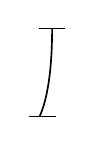
\begin{tikzpicture}[x=.01cm,y=-.01cm,line width=.6pt]
\draw (29,18)--(62,18);
\draw (46,18) .. controls (46,66) and (41,106) .. (30,130);
\draw (16,130)--(51,130);
\end{tikzpicture}}\endgroup\par
Vertical mark with transverse strokes to the left of the reference to the lectures.}
\end{GelfandAdjacentEvidence}
\begin{GelfandAdjacentEvidence}{GELFAND-P000850}{11}


\[
\Phi(A,B)=\Psi_{\alpha_1,\ldots,\alpha_{2A},\dot\alpha_1,\ldots,\dot\alpha_{2B}} \tag{14}
\]
\Unclear{GELFAND-P000850}{phi-overwrite}{The letter in (14) is set as \(\Phi\). It is unclear whether the top stroke is a separate bar.}
\end{GelfandAdjacentEvidence}
\begin{GelfandAdjacentEvidence}{GELFAND-P000850}{12}


The eqs. cont. a bunch of different eqs. — Maxwell, de Wit, Schwinger, Einstein, Hodge–de Rham (for diff. forms).
\Unclear{GELFAND-P000850}{final-list}{The surname after “de Wit” is provisionally read «Швингер» (“Schwinger”).}
\end{GelfandAdjacentEvidence}


(see [3])


\Needspace{7\baselineskip}
\begin{GelfandAdjacentEvidence}{GELFAND-P000851}{1}
\SourcePage{GELFAND-P000851}{unlabelled}
The spinor is symmetr. for now (corresp. irred. repr.). Definition of \(\Delta\).
\Unclear{GELFAND-P000851}{spinor-opening}{The abbreviation before “irred.” is provisionally read «соотв.» (“corresp.”).}
\end{GelfandAdjacentEvidence}
\begin{GelfandAdjacentEvidence}{GELFAND-P000851}{2}

\[
\begin{aligned}
(\Delta\phi)_{\alpha_1\ldots\alpha_{2A},\dot\alpha_1\ldots\dot\alpha_{2B}}
&=\bigl(-\Box\epsilon_{\alpha_1\beta}
+2\nabla_{\dot\xi(\alpha_1}\nabla^{\dot\xi}_{\beta)}\bigr)\\[-.15em]
&\qquad{}\bar\phi^{\beta}{}_{\alpha_2\ldots\alpha_{2A},\dot\alpha_1\ldots\dot\alpha_{2B}}.
\end{aligned}\tag{15}
\]
\Unclear{GELFAND-P000851}{delta-operator-indices}{The small dots in the contraction are provisionally assigned to the two \(\xi\) indices. Parentheses enclose the lower \(\alpha_1,\beta\).}
\end{GelfandAdjacentEvidence}
\begin{GelfandAdjacentEvidence}{GELFAND-P000851}{3}

\Unclear{GELFAND-P000851}{delta-barred-field}{The right-hand side of (15) is provisionally set with \(\bar\phi^\beta\). A short bar is visible above the letter.}
\end{GelfandAdjacentEvidence}
\begin{GelfandAdjacentEvidence}{GELFAND-P000851}{4}


\uline{Properties}.
\[
1)\qquad(\phi,\Delta\phi)=(\Delta\phi,\phi)\tag{16}
\]
\[
2)\qquad \Delta\phi(0,0)=-\Box\phi,\qquad
\text{here}\quad\Box=\nabla_{\alpha\dot\alpha}\nabla^{\alpha\dot\alpha},\tag{17}
\]
\[
\nabla_{\alpha\dot\alpha}=\sigma^a_{\alpha\dot\alpha}\mathcal{D}_a;
\qquad \mathcal{D}_a=\partial_a+B_a
\]

3) Dirac \(\phi(1/2,0)\) (in curved sp.)
\[
\Psi_\pm=(1\pm\gamma_5)\Psi,\tag{18}
\]
\Unclear{GELFAND-P000851}{dirac-projection}{A short horizontal stroke follows 5. Its function is unclear.}
\end{GelfandAdjacentEvidence}
\begin{GelfandAdjacentEvidence}{GELFAND-P000851}{5}

\(\Psi\) — 4-compon. Dirac spinor
\[
\Delta\Psi_\pm=\left(-\Box+\frac14R\right)\Psi_\pm
\]
\SourceFigure{GELFAND-P000851}{scalar-curvature-marker}{%
\begingroup\color{black}\GelfandFitDiagram{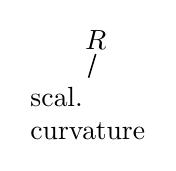
\begin{tikzpicture}[every node/.style={inner sep=1pt},line width=.55pt]
\node (r) at (0,0) {\(R\)};
\draw (0,-.18)--(-.09,-.48);
\node[align=left,anchor=north] at (-.10,-.56) {scal.\\curvature};
\end{tikzpicture}}\endgroup\par
A stroke beneath \(R\) points to the label.}
\end{GelfandAdjacentEvidence}
\begin{GelfandAdjacentEvidence}{GELFAND-P000851}{6}


4) Maxwell in harm. gauge
\Unclear{GELFAND-P000851}{maxwell-gauge-abbreviation}{The abbreviation before “gauge” is provisionally read «гарм.» (“harm.”).}
\end{GelfandAdjacentEvidence}
\begin{GelfandAdjacentEvidence}{GELFAND-P000851}{7}

\[
\Delta A_a=(-\Box g_{ab}+R_{ab})A^b,\qquad
\mathcal{D}^aA_a=0\tag{19}
\]
\Unclear{GELFAND-P000851}{maxwell-overwritten-operator}{The operator before \(A_a\) is heavily overwritten. It is provisionally set as \(\mathcal{D}\). \(\nabla\) is possible.}
\end{GelfandAdjacentEvidence}
\begin{GelfandAdjacentEvidence}{GELFAND-P000851}{8}

\[
5)\qquad\underline{s=\frac32}\qquad\text{somebody and Schwinger}\tag{20}
\]
\Unclear{GELFAND-P000851}{schwinger-line}{The opening words are provisionally read «кого то» (“somebody”). The name before “and Schwinger” is left unspecified.}
\end{GelfandAdjacentEvidence}
\begin{GelfandAdjacentEvidence}{GELFAND-P000851}{9}

\[
6)\quad\underline{s=2}\quad\text{Einstein}\tag{21}
\]
\[
7)\qquad w=\frac1{p!}\omega_{\mu_1\ldots\mu_p}\,dx^{\mu_1}\wedge\ldots\wedge dx^{\mu_p}\tag{22}
\]
\Unclear{GELFAND-P000851}{differential-forms-first-symbol}{The sign left of the equals sign resembles Latin \(w\). The indexed symbol at right is \(\omega\).}
\end{GelfandAdjacentEvidence}
\begin{GelfandAdjacentEvidence}{GELFAND-P000851}{10}

\[
\phi(0,0),\quad\phi(1/2,1/2),\quad\phi(1,0),\quad\phi(0,1)
\]
\[
\Delta=\delta d+d\delta
\]

[crossed out: \sout{…}] Stand. theory of diff. forms descr. \uuline{bosons}.
\Incomplete{GELFAND-P000851}{before-standard-cancelled}{A sign before “Stand.” is crossed out. Its original form is illegible.}
\end{GelfandAdjacentEvidence}
\begin{GelfandAdjacentEvidence}{GELFAND-P000851}{11}


If there were odd ones — then all of math.
\Unclear{GELFAND-P000851}{whole-mat}{The line ends with «мат.» (“math.”) and breaks off.}
\end{GelfandAdjacentEvidence}
\begin{GelfandAdjacentEvidence}{GELFAND-P000851}{12}


[3] — they attached even ind. to the form.
\Unclear{GELFAND-P000851}{before-indices}{The last adjective is provisionally read «чётные» (“even”). Its opening strokes are faint.}
\end{GelfandAdjacentEvidence}
\begin{GelfandAdjacentEvidence}{GELFAND-P000851}{13}


\uwave{Needed}: make anticommuting \(dx\).

[At right:] Berezin did part of it.

There are as yet no [crossed out: \sout{… …}]
\Incomplete{GELFAND-P000851}{after-poka-cancelled}{The two crossed-out words after “no” are illegible.}
\end{GelfandAdjacentEvidence}

diff. forms cont. among the \(dx\) \uwave{comm. and anticomm. ones}

introduce the operator \(\Delta\) and construct an \uwave{index theor.}

The boson field \(\Psi_a\) gives the form \(\Psi_a dx^a\).

For spin \(\frac52\) none of the eqs. will do (one cannot construct the interaction)

— „ — \(\frac32\) it has just been done (supergravity)

\uwave{Idea of I. M. G.} possibly, it need not be \(d\delta+\delta d\).


\Needspace{7\baselineskip}
\begin{GelfandAdjacentEvidence}{GELFAND-P000852}{1}
\SourcePage{GELFAND-P000852}{3}
Equivalent form of the expression for \(\Delta\):
\[
\Delta=-\Box+X,\tag{23}
\]
\[
X=-\Sigma^{ab}R_{ab}^{cd}\Sigma_{cd},\qquad A+B\text{ — integer}\tag{24}
\]
\[
X=-\frac{1}{A}\Sigma^{ab}R_{+ab}^{cd}\Sigma_{cd},\qquad
A+B\text{ — half-integer},\quad A>B.\tag{25}
\]
\Unclear{GELFAND-P000852}{half-integer-abbreviation}{The letter \(B\) in \(A+B\) is heavily retraced. Its underlying form is indistinguishable.}
\end{GelfandAdjacentEvidence}
\begin{GelfandAdjacentEvidence}{GELFAND-P000852}{2}

\SourceFigure{GELFAND-P000852}{curvature-insertion}{%
\begingroup\color{black}\GelfandFitDiagram{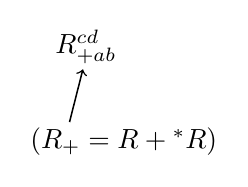
\begin{tikzpicture}[line width=.55pt,every node/.style={inner sep=1pt}]
\node at (0,1.2) {\(R_{+ab}^{cd}\)};
\node at (.48,0) {\((R_+=R+{}^*R)\)};
\draw[->] (-.21,.25)--(-.04,.92);
\end{tikzpicture}}\endgroup\par
The arrow runs from the insertion to the overwritten lower sign at \(R\) in (25).}
\end{GelfandAdjacentEvidence}
\begin{GelfandAdjacentEvidence}{GELFAND-P000852}{3}


\(\varphi\) is symmetric here in \(\alpha_1\ldots\alpha_{2A}\) and in \(\dot\alpha_1\ldots\dot\alpha_{2B}\).
\[
\Delta\varphi=\lambda\varphi\tag{26}
\]
\Unclear{GELFAND-P000852}{eigenfield-overwrite}{The sign after \(\Delta\) in (26) is overwritten. It is provisionally set as \(\varphi\).}
\end{GelfandAdjacentEvidence}
\begin{GelfandAdjacentEvidence}{GELFAND-P000852}{4}


The compatibility condition will follow from this.
\SourceFigure{GELFAND-P000852}{circled-symmetry-insertion}{%
\begingroup\color{black}\GelfandFitDiagram{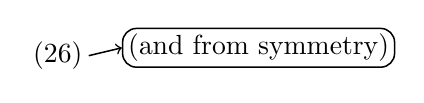
\begin{tikzpicture}[line width=.55pt,every node/.style={inner sep=2pt}]
\node (old) at (0,-.04) {\sout{(26)}};
\node[draw,rounded corners=5pt] (sym) at (2.55,.06) {(and from symmetry)};
\draw[->] (old.east)--(sym.west);
\end{tikzpicture}}\endgroup\par
The stroke through the crossed-out number (26) becomes an arrow to the circled insertion.}
\end{GelfandAdjacentEvidence}
\begin{GelfandAdjacentEvidence}{GELFAND-P000852}{5}


\uwave{Compatibility condition}:
\[
\nabla_{\dot\alpha}^{(\alpha_1}\nabla^{\alpha_2)\dot\alpha}
\varphi_{\alpha_1\alpha_2\ldots\alpha_{2A},\dot\alpha_1\ldots\dot\alpha_{2B}}=0
\tag{27}
\]
\Unclear{GELFAND-P000852}{equation27-number}{The last digit is overwritten. The label is provisionally set as (27). (28) is possible.}
\end{GelfandAdjacentEvidence}
\begin{GelfandAdjacentEvidence}{GELFAND-P000852}{6}

\(A\leq1\), \(B\leq1\) \(\Rightarrow\) the case of all phys. fields

Consider the heat eq.
\[
\frac{d}{dt}F(x,x',t)+\Delta F(x,x',t)=0,\qquad
F\big|_{t=0}=\delta(x-x').\tag{28}
\]
on a compact man.
\[
\operatorname{Tr}F(x,x,t)\underset{t\to+0}{\sim}
\sum_{k=0}^{\infty}b_k\,t^{(k-4)/2}\tag{29}
\]
\Unclear{GELFAND-P000852}{equation29-coefficient-edit}{There is an overwritten mark before \(t\), possibly a crossed-out \((x)\).}
\end{GelfandAdjacentEvidence}
\begin{GelfandAdjacentEvidence}{GELFAND-P000852}{7}

\Incomplete{GELFAND-P000852}{equation29-exponent-deletion}{The earlier writing before the exponent \((k-4)/2\) is crossed out and illegible.}
\end{GelfandAdjacentEvidence}
\begin{GelfandAdjacentEvidence}{GELFAND-P000852}{8}

\[
B_k=\int d^4x\sqrt{g}\,b_k,\tag{30}
\]
Then
\[
B_4=n+m.\tag{31}
\]
[At right:] \(B_4\) — the first nondivergent one.

\(n\) — number of zero eigenval. (26)

\(m\) — [crossed out: \sout{number of nonzero eigenval.}]
[Inserted below:] multiplicity of a nonzero (any) eigenval.

[At right:] [their common multiplicity — all multiplicities are the same!!]
\SourceFigure{GELFAND-P000852}{multiplicity-correction}{%
\begingroup\color{black}\GelfandFitDiagram{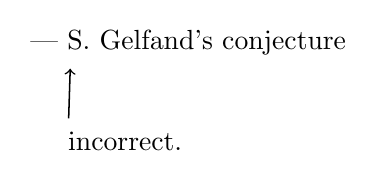
\begin{tikzpicture}[line width=.55pt,every node/.style={inner sep=1pt}]
\node[anchor=west] at (0,1.25) {— S. Gelfand’s conjecture};
\node[anchor=west] at (.48,0) {\uwave{incorrect.}};
\draw[->] (.53,.29)--(.55,.92);
\end{tikzpicture}}\endgroup\par
An arrow from the underlined “incorrect” points upward to the conjecture.}
\end{GelfandAdjacentEvidence}
\begin{GelfandAdjacentEvidence}{GELFAND-P000852}{9}


Aim — expr. in terms of top. invariants.

\uwave{Gilkey} got as far as \(\underline{\underline{B_6}}\). (1975)
\Unclear{GELFAND-P000852}{gilkey-coefficient}{The overwritten letter is provisionally set as \(B\). \(b\) is possible.}
\end{GelfandAdjacentEvidence}
\begin{GelfandAdjacentEvidence}{GELFAND-P000852}{10}


\SourceFigure{GELFAND-P000852}{gilkey-leaders}{%
\begingroup\color{black}\GelfandFitDiagram{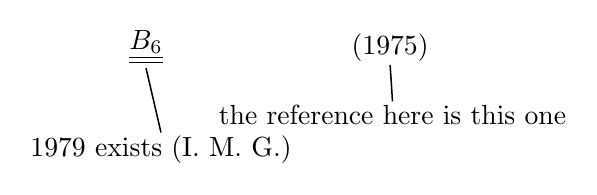
\begin{tikzpicture}[line width=.55pt,every node/.style={inner sep=1pt}]
\node (b) at (0,1.1) {\(\underline{\underline{B_6}}\)};
\node (d) at (3.10,1.1) {(1975)};
\node (y) at (.19,-.2) {1979 exists (I. M. G.)};
\node (r) at (3.13,.25) {the reference here is this one};
\draw (b.south)--(y.north);
\draw (d.south)--(r.north);
\end{tikzpicture}}\endgroup\par
Two short strokes link the upper symbols to the notes beneath them.}
\end{GelfandAdjacentEvidence}
\begin{GelfandAdjacentEvidence}{GELFAND-P000852}{11}

\Unclear{GELFAND-P000852}{gilkey-year-word}{The word after 1979 is provisionally read «есть» (“exists”). «ещё» (“also”) is possible.}
\end{GelfandAdjacentEvidence}
\begin{GelfandAdjacentEvidence}{GELFAND-P000852}{12}

\Unclear{GELFAND-P000852}{gilkey-reference-word}{The last word after “the reference here” is provisionally read «такая» (“this one”).}
\end{GelfandAdjacentEvidence}
\begin{GelfandAdjacentEvidence}{GELFAND-P000852}{13}


If there is a boundary, then likewise \(b_4\) now [crossed out: \sout{…}] recently written up; the question is consid. difficult.
\Unclear{GELFAND-P000852}{boundary-coefficient}{The coefficient on the line about the boundary is provisionally read as \(b_4\).}
\end{GelfandAdjacentEvidence}
\begin{GelfandAdjacentEvidence}{GELFAND-P000852}{14}

\Incomplete{GELFAND-P000852}{boundary-deleted-word}{The word before “recently” is crossed out and illegible.}
\end{GelfandAdjacentEvidence}
\begin{GelfandAdjacentEvidence}{GELFAND-P000852}{15}


Consid. reducible reprs.
\[
\varphi_{\alpha\beta}=\varphi_{(\alpha\beta)}
+\frac12\varepsilon_{\alpha\beta}\varphi_{\alpha}^{\alpha}\tag{32}
\]
\[
[1,0]=(1,0)\oplus(0,0)
\]
By the compatibility conditions
\[
[\nabla_{\alpha}^{\dot\alpha},\Delta]\varphi[A,B]=0\tag{33}
\]
\Unclear{GELFAND-P000852}{compatibility-commutator}{There is a small stroke above the upper \(\alpha\). It is provisionally taken as a dot.}
\end{GelfandAdjacentEvidence}



\Needspace{7\baselineskip}
\begin{GelfandAdjacentEvidence}{GELFAND-P000853}{1}
\SourcePage{GELFAND-P000853}{unlabelled}
\[
(\Delta-\lambda)\varphi_{\alpha_1\ldots}=0\tag{34}
\]
Consid.
\[
\begin{aligned}
\Psi_{\alpha_1\ldots\alpha_{2A-1}\dot\alpha_1\ldots\dot\alpha_{2B+1}}
={}&\nabla_{\dot\alpha_{2B+1}}^{\alpha_{2A}}\\[-.15em]
&\qquad\varphi_{\alpha_1\ldots\alpha_{2A}\dot\alpha_1\ldots\dot\alpha_{2B}}
\end{aligned}\tag{35}
\]
\Unclear{GELFAND-P000853}{equation35-dot-order}{In (35) the dot belongs to the lower derivative index. The upper index is provisionally read as \(\alpha_{2A}\).}
\end{GelfandAdjacentEvidence}
\begin{GelfandAdjacentEvidence}{GELFAND-P000853}{2}


\(\Psi\ne0\) when \(\varphi\ne0\) (otherwise \(\overset{\circ}{\times}\) with (34)).
\Unclear{GELFAND-P000853}{after35-symbol}{The small oval above the diagonal cross is provisionally set as a circle. The meaning of the mark is unclear.}
\end{GelfandAdjacentEvidence}
\begin{GelfandAdjacentEvidence}{GELFAND-P000853}{3}

\[
m[A,B]=m[A-\tfrac12,B+\tfrac12]\tag{36}
\]
\SourceFigure{GELFAND-P000853}{nonzero-modes-leader}{%
\begingroup\color{black}\GelfandFitDiagram{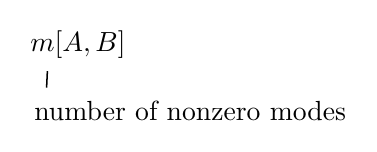
\begin{tikzpicture}[line width=.55pt,every node/.style={inner sep=1pt}]
\node[anchor=west] at (-.05,.85) {\(m[A,B]\)};
\draw (.21,.51)--(.20,.30);
\node[anchor=west] at (0,0) {number of nonzero modes};
\end{tikzpicture}}\endgroup\par
A short stroke below \(m\) points to the label.}
\end{GelfandAdjacentEvidence}
\begin{GelfandAdjacentEvidence}{GELFAND-P000853}{4}

\[
A+B=S,\qquad A-B=T.
\]
Then we get
\[
m[S,T]=m[S]\tag{37}
\]
Hence
\[
n[S,T]-n[S,T']=B_4[S,T]-B_4[S,T']\tag{38}
\]
\[
n[S,T]-n[S,T-1]=4^{s-1}\bigl((T-\tfrac12)\chi+(s-\tfrac23)\tfrac{p}{2}\bigr)\tag{39}
\]
\Unclear{GELFAND-P000853}{index39-lettercase}{The two letters at right in (39) are provisionally read as lowercase \(s\). The notation at left looks like uppercase \(S\).}
\end{GelfandAdjacentEvidence}
\begin{GelfandAdjacentEvidence}{GELFAND-P000853}{5}


\(\chi\) — Euler number, \(p\) — Pontryagin number

\uwave{On the heat eq}.
\Unclear{GELFAND-P000853}{heat-heading}{The end of the underlined heading is provisionally read «теплопров.» (“heat”).}
\end{GelfandAdjacentEvidence}
\begin{GelfandAdjacentEvidence}{GELFAND-P000853}{6}

\[
F(x,x',t)=\sum_{i=0}^{\infty}\varphi_i(x)\varphi_i(x')e^{-\lambda_i t}\tag{40}
\]
\(\varphi_i\) — orthonorm. syst.
\[
F(x,x',0)=\delta(x,x')\tag{41}
\]
\[
\int_M d^4x\sqrt{g}\,F(x,x,t)
=\sum_{i=0}^{\infty}e^{-\lambda_i t}
=n+\sum_{i=n+1}^{\infty}e^{-\lambda_i t}\tag{42}
\]
\Unclear{GELFAND-P000853}{equation42-deleted-mark}{There is a small blacked-out mark above the second \(x\), possibly a prime.}
\end{GelfandAdjacentEvidence}
\begin{GelfandAdjacentEvidence}{GELFAND-P000853}{7}

\[
F(x,x,t)\sim\sum_{k=0}^{\infty}b_k(x)t^{(k-4/2}\tag{43}
\]
\Unclear{GELFAND-P000853}{equation43-exponent}{The 4 is overwritten. A separate closing parenthesis before the fraction slash cannot be distinguished.}
\end{GelfandAdjacentEvidence}
\begin{GelfandAdjacentEvidence}{GELFAND-P000853}{8}


\(m\) is determ. from this!! — by discarding the diverg. terms of \(\sum e^{-\lambda_i t}\) and \(n\) \uline{contributes}.

\uwave{\(m\) — regulariz. sum}
\Unclear{GELFAND-P000853}{regularized-sum}{The abbreviation in the underlined note is provisionally read «регуляриз.» (“regulariz.”).}
\end{GelfandAdjacentEvidence}
\begin{GelfandAdjacentEvidence}{GELFAND-P000853}{9}


“\(m\) — is an integer (!) on deep top. grounds ”

These are the stand. one-loop diverg. of the cont. integral.
\Unclear{GELFAND-P000853}{integral-abbreviation}{The Russian end of the line is provisionally read «контин. интеграла». The last word looks like a genitive form.}
\end{GelfandAdjacentEvidence}
\begin{GelfandAdjacentEvidence}{GELFAND-P000853}{10}


[At right: в?]
\Unclear{GELFAND-P000853}{isolated-mark}{The isolated dark sign may be the letter «в». Its reading is uncertain.}
\end{GelfandAdjacentEvidence}
\begin{GelfandAdjacentEvidence}{GELFAND-P000853}{11}


Def. \(\chi\) and \(p\) for manifs. without boundary
\[
\chi=\int {}^*R_{abcd}\,{}^*R^{abcd}\,d^4x\sqrt{g}\tag{44}
\]
\Unclear{GELFAND-P000853}{curvature-stars}{Stars are visible before both occurrences of \(R\) in (44).}
\end{GelfandAdjacentEvidence}

\[
p=\int {}^*R_{abcd}R^{abcd}\,d^4x\,\sqrt{g}\tag{45}
\]


\Needspace{7\baselineskip}
\begin{GelfandAdjacentEvidence}{GELFAND-P000854}{1}
\SourcePage{GELFAND-P000854}{4}
\uline{8.10.79.} \quad \uline{Gelfand Sem.}

\uline{Draft theor. minimum}, \uline{needed in any specialization}. (for 1st-year students)

1. \uline{Algebra}

van der Waerden, chs. 1–5, 12.

Gelfand lectures on lin. algebra

Atiyah, Macdonald

2. \uline{Analysis}
\SourceFigure{GELFAND-P000854}{analysis-reading-braces}{%
\(\underline{\text{or}}\quad
\left\{\begin{array}{l}
\text{Bers}\\
\text{[crossed out: \sout{…}] Luzin}\\
\text{Berman}
\end{array}\right\}\)
\par\noindent for technical institutes.
\par\smallskip
then.
\par\noindent
\(\text{or}\quad
\left\{\begin{array}{l}
\text{Rudin}\\
\text{Dieudonné}\\
\text{Grauert, Lieb, Fischer}\\
\text{Schwartz}
\end{array}\right\}\)
\par\noindent
[At right:]\par
Spivak\par
Bishop–Crittenden\par
Nomizu
\par Two pairs of braces group the lists. Three separate lines stand to the right of the second pair.}
\end{GelfandAdjacentEvidence}
\begin{GelfandAdjacentEvidence}{GELFAND-P000854}{2}

\Unclear{GELFAND-P000854}{analysis-cancelled-name}{A surname is crossed out before “Luzin.” “Berman” is a possible reading.}
\end{GelfandAdjacentEvidence}
\begin{GelfandAdjacentEvidence}{GELFAND-P000854}{3}


\uline{Check question:} calculate approximately
\[
\begin{aligned}
&\int_{-\infty}^{\infty} e^{-x^2}\cos 1000x\,dx,\qquad
 \int_{-\infty}^{\infty} e^{-1000x^2}\cos x\,dx\\
&\qquad\text{(and comp. with tables)}\\[.3em]
&\int_{-\infty}^{\infty} e^{-1000x^4}\cos x\,dx,\qquad
 \int_{-\infty}^{\infty} e^{-x^4}\cos 1000x\,dx
\end{aligned}
\]

3. \uline{Arnold} \(\mathrm{I},\ \mathrm{II},\ \mathrm{III}.\)

4. \uline{Kirillov} \(\tfrac12+\tfrac12\)

\uline{Serre} lin. reprs. of finite groups

(he does not understand the 3rd chapter)

\uline{Generalized fns.} \(\mathrm{I}\) issue, chs. 1–2

5. \uline{Know the partial differential equations}. (there is nothing to read).

\uwave{Check problem in lin. algebra:}

\uwave{find the can. form of a self-adj. oper. in a [crossed out: \sout{…}] symplect. space}.
\Incomplete{GELFAND-P000854}{symplectic-deleted-word}{The word after “in” is crossed out and illegible.}
\end{GelfandAdjacentEvidence}
\begin{GelfandAdjacentEvidence}{GELFAND-P000854}{4}

\Unclear{GELFAND-P000854}{symplectic-final-abbreviation}{The abbreviation after the crossed-out word is provisionally read «симплект.» (“symplect.”).}
\end{GelfandAdjacentEvidence}
\begin{GelfandAdjacentEvidence}{GELFAND-P000854}{5}


6. [blacked out] \uline{Spec. theory of rel. \(+\) GR}
\Unclear{GELFAND-P000854}{reading6-blackened-mark}{A single sign before “Spec.” is blacked out. It may be the letter «А».}
\end{GelfandAdjacentEvidence}
\begin{GelfandAdjacentEvidence}{GELFAND-P000854}{6}


\(+\) \uline{geometry}

[At right:] Landau, Lifshitz ( vol. 2)

jointly with Nomizu
\Unclear{GELFAND-P000854}{nomizu-note-abbreviation}{The abbreviation before “with Nomizu” is provisionally read «совм.» (“jointly”).}
\end{GelfandAdjacentEvidence}
\begin{GelfandAdjacentEvidence}{GELFAND-P000854}{7}


\medskip
\uuline{S. Gindikin}. \uline{Beginnings of twistor theory}.

To be presented in the language of integr. geometry.

[At right:] Twistors were introduced by \uline{Penrose}.

see one of the recent issues of BAMS,

1979, vol. 1 (new series),

art. by \uline{Wells} (\uline{Wells.})

[crossed out: \sout{… let us consider?}]
\Incomplete{GELFAND-P000854}{cancelled-before-diagram}{The crossed-out line before (1) cannot be read in full. The last word is provisionally read «рассмотрим» (“let us consider”).}
\end{GelfandAdjacentEvidence}
\begin{GelfandAdjacentEvidence}{GELFAND-P000854}{8}


\SourceFigure{GELFAND-P000854}{twistor-projection}{%
\begingroup\color{black}\GelfandFitDiagram{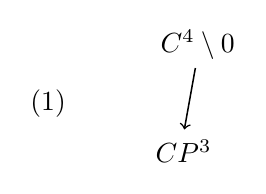
\begin{tikzpicture}[line width=.55pt,every node/.style={inner sep=1pt}]
\node at (-.9,.61) {(1)};
\node (c) at (1,1.35) {\(\mathbb{C}^4\setminus0\)};
\node (p) at (.82,0) {\(\mathbb{C}P^3\)};
\draw[->] (.97,1.06)--(.83,.28);
\end{tikzpicture}}\endgroup}
\end{GelfandAdjacentEvidence}
\begin{GelfandAdjacentEvidence}{GELFAND-P000854}{9}


In \(\mathbb{C}^4\) fix a Hermitian form [blacked out] \((++--)\). \(\langle\ ,\ \rangle\).
\Incomplete{GELFAND-P000854}{hermitian-blackened-symbol}{A sign is blacked out before the parentheses with the signature. It is illegible.}
\end{GelfandAdjacentEvidence}


We obtain \(\alpha\)-twistors: elements of \(\mathbb{C}P^3\) or corresp. elems. of \(\mathbb{C}^4\).

\((\mathbb{C}P^3)'\) — dual sp.. A form arises there too, and these are — \(\beta\)-twistors.


\Needspace{7\baselineskip}
\begin{GelfandAdjacentEvidence}{GELFAND-P000855}{1}
\SourcePage{GELFAND-P000855}{unlabelled}
\[
\begin{aligned}
\langle z,z\rangle>0&\Rightarrow\text{pos. twistor}\\
\langle z,z\rangle=0&\Rightarrow\text{null — „ —}\\
\langle z,z\rangle<0&\Rightarrow\text{neg. — „ —}
\end{aligned}
\]
In \(\mathbb{C}P^3\) consid. lines (2-dim. subsp. in \(\mathbb{C}^4\)).
Their set: \(G=G_{4,2}=G_{4,2}^{\mathbb{C}}\).

Over \(G\) there is a natural princ. bundle of 2-frames in \(\mathbb{C}^4\):
\Unclear{GELFAND-P000855}{bundle-word}{The word before “bundle” is provisionally read «натурельное» (“natural”). Its middle and final strokes run together.}
\end{GelfandAdjacentEvidence}
\begin{GelfandAdjacentEvidence}{GELFAND-P000855}{2}

\SourceFigure{GELFAND-P000855}{bundle-projection}{%
\begingroup\color{black}\GelfandFitDiagram{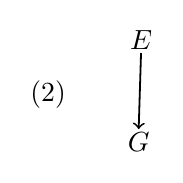
\begin{tikzpicture}[line width=.65pt,every node/.style={inner sep=1pt}]
\node at (-1.18,.61) {(2)};
\node (e) at (0,1.30) {\(E\)};
\node (g) at (-.03,0) {\(G\)};
\draw[->] (e.south)--(g.north);
\end{tikzpicture}}\endgroup}
\end{GelfandAdjacentEvidence}
\begin{GelfandAdjacentEvidence}{GELFAND-P000855}{3}


[Crossed out above the heading: \sout{In \(\mathbb{C}^4\) …}]
\Incomplete{GELFAND-P000855}{cancelled-heading-line}{The crossed-out line may begin «В \(\mathbb C^4\)» (“In \(\mathbb C^4\)”). The full line is illegible.}
\end{GelfandAdjacentEvidence}
\begin{GelfandAdjacentEvidence}{GELFAND-P000855}{4}


[Crossed out at left: \sout{…}] \uwave{Coordinates in \(G\)}.
\Incomplete{GELFAND-P000855}{cancelled-heading-prefix}{A separate short entry at the left of the heading is crossed out and illegible.}
\end{GelfandAdjacentEvidence}
\begin{GelfandAdjacentEvidence}{GELFAND-P000855}{5}


Choose in \(\mathbb{C}^4\) 2 planes (transvers.) \(L\) and \(L'\), then any other is a graph,
the matrix of the corresp. transf. gives coordinates.
\SourceFigure{GELFAND-P000855}{inserted-planes}{%
\begingroup\color{black}\GelfandFitDiagram{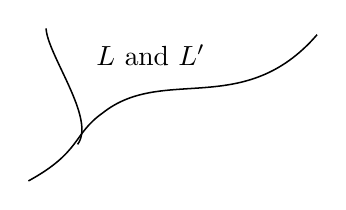
\begin{tikzpicture}[x=.016cm,y=-.016cm,line width=.55pt,every node/.style={inner sep=1pt}]
\node at (130,41) {\(L\) and \(L'\)};
\draw (47,20) .. controls (48,41) and (87,92) .. (72,112);
\draw (33,141) .. controls (75,118) and (68,104) .. (92,87)
 .. controls (140,49) and (204,92) .. (262,25);
\end{tikzpicture}}\endgroup\par
The insertion mark leads to the plane labels above the line.}
\end{GelfandAdjacentEvidence}
\begin{GelfandAdjacentEvidence}{GELFAND-P000855}{6}


Choose in [crossed out: \sout{…}] \(L\) basis \(e_0\ e_1\); In \(L'\) basis \(e_3,e_4\).
\Incomplete{GELFAND-P000855}{cancelled-before-l}{The entry before \(L\) is crossed out and illegible.}
\end{GelfandAdjacentEvidence}
\begin{GelfandAdjacentEvidence}{GELFAND-P000855}{7}

Then if \(\widetilde L\in G_{4,2}\), then in \(\widetilde L\) there is a basis of the form
\Unclear{GELFAND-P000855}{plane-symbol-under-formula}{The repeated plane symbol is heavily retraced. It is provisionally set as \(\widetilde L\).}
\end{GelfandAdjacentEvidence}
\begin{GelfandAdjacentEvidence}{GELFAND-P000855}{8}

\[
\begin{cases}
f_0=e_0+u_{03}e_3+u_{04}e_4\\
f_1=e_1+u_{13}e_3+u_{14}e_4
\end{cases}\tag{3}
\]
\Unclear{GELFAND-P000855}{formula-3-index}{The first subscript of \(u\) before \(e_3\) in the second line is provisionally read as 1. The numeral has been retraced.}
\end{GelfandAdjacentEvidence}
\begin{GelfandAdjacentEvidence}{GELFAND-P000855}{9}

\(u_{ij}\) — coordinates.

Let \(L,L'\) be transvers. and isotropic with resp. to \(\langle\cdot,\cdot\rangle\).
\uline{Problem}. Such \(L\) and \(L'\) exist.
\[
\{e_A,\ A=0,1\}\text{ — basis in } L.\tag{4}
\]
In \(L'\) introduce a basis
\[
\{e^{A'},\ A'=0',1'\}\text{ — basis in } L'\tag{5}
\]

[crossed out: \sout{…}] [above the line: Let [crossed out: \sout{…}]]
the form [above the line: \(\langle\ ,\ \rangle\)] in the basis
\((e_0,e_1,e^{0'},e^{1'})\) have [crossed out: \sout{…}] the matrix
\Incomplete{GELFAND-P000855}{cancelled-form-prefix}{The entry before “the form” on the main line is crossed out and illegible.}
\end{GelfandAdjacentEvidence}
\begin{GelfandAdjacentEvidence}{GELFAND-P000855}{10}

\Incomplete{GELFAND-P000855}{cancelled-after-pust}{A short mark after the inserted “Let” is crossed out and illegible.}
\end{GelfandAdjacentEvidence}
\begin{GelfandAdjacentEvidence}{GELFAND-P000855}{11}

\Incomplete{GELFAND-P000855}{cancelled-before-matrix}{The word between “have” and “the matrix” is crossed out and illegible.}
\end{GelfandAdjacentEvidence}
\begin{GelfandAdjacentEvidence}{GELFAND-P000855}{12}

\SourceFigure{GELFAND-P000855}{form-insertions}{%
\begingroup\color{black}\GelfandFitDiagram{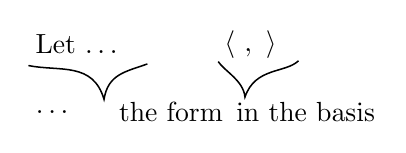
\begin{tikzpicture}[line width=.55pt,every node/.style={inner sep=1pt}]
\node at (.38,.83) {Let \sout{…}};
\node at (2.56,.83) {\(\langle\ ,\ \rangle\)};
\draw (-.26,.56) .. controls (.14,.48) and (.56,.61) .. (.70,.13)
 .. controls (.75,.45) and (.97,.48) .. (1.25,.58);
\draw (2.15,.61) .. controls (2.23,.49) and (2.47,.37) .. (2.49,.16)
 .. controls (2.62,.54) and (3.00,.46) .. (3.17,.62);
\node at (.07,-.03) {\sout{…}};
\node at (1.55,-.03) {the form};
\node at (3.26,-.03) {in the basis};
\end{tikzpicture}}\endgroup\par
Two marks give the insertion points for “Let” and the angle brackets.}
\end{GelfandAdjacentEvidence}
\begin{GelfandAdjacentEvidence}{GELFAND-P000855}{13}

\[
\begin{pmatrix}0&iE\\-iE&0\end{pmatrix};\tag{6}
\]
i.e.
\[
\langle e_0,e^{0'}\rangle=\langle e_1,e^{1'}\rangle=i,
\qquad\text{the other scal. prod. }=0\tag{7}
\]
Make a change of variables in \(L\):
\[
\widetilde e_B=g_B^A e_A\tag{8}
\]
Then it is easy to check that
\[
e^{A'}\text{ transf. by means of }(g^*)^{-1}\tag{9}
\]
(follows from the relat. of [crossed out: \sout{…}] orthogonality)
\Incomplete{GELFAND-P000855}{cancelled-orthogonality-word}{The entry before “orthogonality” is crossed out and illegible.}
\end{GelfandAdjacentEvidence}
\begin{GelfandAdjacentEvidence}{GELFAND-P000855}{14}


There are other transf. laws:
[Crossed out at left: \sout{…}]
\Incomplete{GELFAND-P000855}{cancelled-index-intro}{The mark before the lines with indices is crossed out and illegible.}
\end{GelfandAdjacentEvidence}
\begin{GelfandAdjacentEvidence}{GELFAND-P000855}{15}

\SourceFigure{GELFAND-P000855}{index-transformation-arcs}{%
\begingroup\color{black}\GelfandFitDiagram{\begin{tikzpicture}[line width=.55pt,every node/.style={inner sep=1pt}]
\node at (.22,1.12) {\(A'\)};
\node[anchor=west] at (.58,1.12) {by \(\bar g\)};
\node at (.22,.05) {\(B\)};
\node[anchor=west] at (.58,.05) {— „ — \((g^T)^{-1}\)};
\node at (3.23,1.12) {\(B'\)};
\node[anchor=west] at (3.60,1.12) {by \((g^*)^{-1}\)};
\draw (-.04,.88) .. controls (-.03,1.07) and (.22,1.66) .. (.40,1.47)
 .. controls (.48,1.39) and (.47,1.19) .. (.44,1.01);
\draw (.04,.20) .. controls (-.01,-.43) and (.32,-.17) .. (.47,.17);
\draw (3.03,1.33) .. controls (2.82,.67) and (3.23,.75) .. (3.55,1.26);
\end{tikzpicture}}\endgroup\par
The arc is above \(A'\) and below \(B\) and \(B'\). The meaning of the arcs is unclear.}
\end{GelfandAdjacentEvidence}



\Needspace{7\baselineskip}
\begin{GelfandAdjacentEvidence}{GELFAND-P000856}{1}
\SourcePage{GELFAND-P000856}{5}
\uline{Problem.} Prove that \(U(2,2)\) has a subgroup isom. to \(GL(2,\mathbb{C})\)
(hint: use the preceding result).

Coordinates:
\[
\{z^A,z_{A'}\}\qquad\text{in the basis }\{e_A,e^{A'}\}\tag{10}
\]
\[
z=z^Ae_A+z_{A'}e^{A'}\in\mathbb C^4\tag{11}
\]
\uline{\uline{I.M.G.}} \(\mathbb C^4\ni\lbrace x_1,x_2,x_3,x_4)\).
\Unclear{GELFAND-P000856}{coordinate-tuple-bracket}{The opening mark resembles a brace. The closing mark is a parenthesis.}
\end{GelfandAdjacentEvidence}
\begin{GelfandAdjacentEvidence}{GELFAND-P000856}{2}

\[
\langle x,y\rangle=x_1\bar y_1+x_2\bar y_2-x_3\bar y_3-x_4\bar y_4\tag{12}
\]
\Unclear{GELFAND-P000856}{formula-12-sign}{The mark before the third term is provisionally read as a minus sign. The stroke has been overwritten.}
\end{GelfandAdjacentEvidence}
\begin{GelfandAdjacentEvidence}{GELFAND-P000856}{3}

\(L,L'\) — 2 isotropic subsp. and 2 bases \(\{e_0,e_1\}\); \(\{e^{0'},e^{1'}\}\).
Then
\[
z=z^0e_0+z^1e_1+z_{0'}e^{0'}+z_{1'}e^{1'}\tag{13}
\]
\[
\{z^A,z_{A'}\}\text{ — spinor coordinates in }\mathbb C^4\tag{14}
\]
Requirement on the basis:
\Unclear{GELFAND-P000856}{basis-requirement}{The initial letter of «Требование» (“Requirement”) is retraced.}
\end{GelfandAdjacentEvidence}
\begin{GelfandAdjacentEvidence}{GELFAND-P000856}{4}

\[
\langle e_0,e^{0'}\rangle=\langle e_1,e^{1'}\rangle=i,
\qquad\text{the other scal. prod.}=0.\tag{15}
\]

\uline{\uline{S.G.}} Let \(\widetilde L\in G\); \(\widetilde L\cap L'=\{0\}\).
Then choose a basis as follows:
\[
f_A=e_A+u_{AB'}e^{B'}\tag{16}
\]
\Unclear{GELFAND-P000856}{formula-16-indices}{The two indices on the left and in the first term on the right are retraced and read as \(A\).}
\end{GelfandAdjacentEvidence}

The spinor indices themselves show how they transform. (worth writing out!)

(Twistor theory in curved space has yet to be worked out, though there are already papers on it).
Consider groups acting in \(\mathbb C^4\).
The action of \(GL(4,\mathbb C)\) carries over to \(G_{4,2}\).
\[
\begin{aligned}
T_+&:\quad\langle z,z\rangle>0\\
T_-&:\quad\langle z,z\rangle<0\\
N&:\quad\langle z,z\rangle=0\qquad\text{— 7-dimensional surface in }\mathbb C^4.
\end{aligned}
\]
\[
\begin{aligned}
S_+&\text{ — 2-dimensional planes }\subset T_+\quad\text{(except 0)}\\
S_-&\text{ — — „ — }\subset T_-\quad\text{(— „ —)}\\
M&\text{ — — „ — }\subset N
\end{aligned}
\]
\(S_+,S_-\) — lie entirely within the range of the coord. \(u_{AB'}\).
\[
\begin{cases}
S_+=\{u:\ \frac{1}{i}(u-u^*)\gg0\}\\
S_-=\{u:\ \frac{1}{i}(u-u^*)\ll0\}
\end{cases}\tag{17}
\]


\Needspace{7\baselineskip}
\begin{GelfandAdjacentEvidence}{GELFAND-P000857}{1}
\SourcePage{GELFAND-P000857}{unlabelled}
\(M\) no longer lies wholly in the coord. neighborhood. Let \(M_0\) — be the part that does lie in it.
\[
M_0=\{u:\ u=u^*\}\tag{18}
\]
\[
\dim_{\mathbb R} M_0=4,\qquad \dim_{\mathbb C} S^\pm=4.
\]
\(M_0\) — the common skeleton of \(S^\pm\).
\[
\partial S_+=\{\text{supporting planes to }T_+\}
\]

Now consider in \(\mathbb C^4\) the group \(U(2,2)\), preserving
[crossed out: \sout{…}] the form
\Incomplete{GELFAND-P000857}{cancelled-before-form}{The entry before “the form” is crossed out and illegible.}
\end{GelfandAdjacentEvidence}
\begin{GelfandAdjacentEvidence}{GELFAND-P000857}{2}

(and, hence, the surface \(N\)). Then it is clear that \(U(2,2)\) preserves all
[crossed out: \sout{…}] the domains \(S_{\pm},M\)
\Incomplete{GELFAND-P000857}{cancelled-before-domains}{The entry before “domains” is crossed out and illegible.}
\end{GelfandAdjacentEvidence}
\begin{GelfandAdjacentEvidence}{GELFAND-P000857}{3}

(canon. construction) and acts on each \uline{transitively}!!
(\uwave{A problem in lin. algebra!})

On \((\mathbb C^4,\langle\ ,\ \rangle)\) acts \(U(2,2)\)
and preserves the whole construction.
\(g\in U(2,2)\) is written in a basis of the kind descr. above:
\[
g=\begin{pmatrix}A&B\\C&D\end{pmatrix}\tag{19}
\]
\uwave{Action on} \(u\):
\[
g:\ u\mapsto (Au+B)(Cu+D)^{-1}\tag{20}
\]
The action makes \(M\) into the conformal compactification of Minkowski space:
the Poincaré gr. \(\subset SU(2,2)\) (addition of conformal transf.).

\SourceFigure{GELFAND-P000857}{g0-incidence}{%
\begingroup\color{black}\GelfandFitDiagram{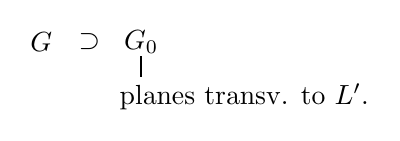
\begin{tikzpicture}[line width=.6pt,every node/.style={inner sep=1pt}]
\node at (0,0) {\(G\)};
\node at (.61,0) {\(\supset\)};
\node at (1.27,0) {\(G_0\)};
\draw (1.27,-.18)--(1.27,-.44);
\node[anchor=north west] at (.95,-.49) {planes transv. to \(L'\).};
\end{tikzpicture}}\endgroup}
\end{GelfandAdjacentEvidence}
\begin{GelfandAdjacentEvidence}{GELFAND-P000857}{4}


Consider the subgroup preserving \(G_0\) (\(\sim\) preserving \(L'\)). This group is isom. to the Poincaré gr.:
\[
u\to aua^*+b\tag{21}
\]
\(a\in GL(2,\mathbb C)\), \(b=b^*\).
\EvidenceBlock{GELFAND-P000857}{poincare-group-source}{The manuscript reads “This group is isom. to the Poincaré gr.” Equation (21) and its parameters follow.}{\GelfandExcerptCaption}
\end{GelfandAdjacentEvidence}
\begin{GelfandAdjacentEvidence}{GELFAND-P000857}{5}


In the notation of (19) here:
\[
A=a,\quad C=0,\quad D=(a^*)^{-1},\quad BD^{-1}=b.\tag{22}
\]
\[
\text{The Minkowski metric on }M_0^{\text{…}}:\qquad \det(du)\tag{23}
\]
\Unclear{GELFAND-P000857}{formula-23-superscript}{The stroke above \(M_0\) is obscured. The superscript is illegible.}
\end{GelfandAdjacentEvidence}
\begin{GelfandAdjacentEvidence}{GELFAND-P000857}{6}

Pauli coord. (on \(M_0\)):
\[
\begin{pmatrix}
u_0-u_1&u_3+i u_4\\
u_3-i u_4&u_1+u_0
\end{pmatrix},\qquad u_j\in\mathbb R\tag{24}
\]
\Unclear{GELFAND-P000857}{formula-24-indices}{The two indices in the upper left entry are retraced and read as \(0\) and \(1\).}
\end{GelfandAdjacentEvidence}



\Needspace{7\baselineskip}
\begin{GelfandAdjacentEvidence}{GELFAND-P000858}{1}
\SourcePage{GELFAND-P000858}{6}
Then the metric takes the form
\[
(du_0)^2-(du_1)^2-(du_2)^2-(du_3)^3.\tag{25}
\]
\Unclear{GELFAND-P000858}{metric-power}{The last term has exponent \(3\) in the manuscript.}
\end{GelfandAdjacentEvidence}
\begin{GelfandAdjacentEvidence}{GELFAND-P000858}{2}

\Unclear{GELFAND-P000858}{metric-first-indices}{The first term reads \(0\). The retraced subscript in the second term reads \(1\).}
\end{GelfandAdjacentEvidence}
\begin{GelfandAdjacentEvidence}{GELFAND-P000858}{3}

\[
M_0=M\cap G_0\underset{\mathrm{def}}{=}\text{ordinary Minkowski space}.\tag{26}
\]
\SourceFigure{GELFAND-P000858}{chart-pointer}{%
\begingroup\color{black}\GelfandFitDiagram{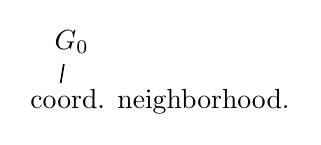
\begin{tikzpicture}[line width=.6pt,every node/.style={inner sep=1pt}]
\node (g) at (0,0) {\(G_0\)};
\draw (-.10,-.28)--(-.14,-.52);
\node[anchor=north west] at (-.57,-.56) {coord. neighborhood.};
\end{tikzpicture}}\endgroup}
\end{GelfandAdjacentEvidence}
\begin{GelfandAdjacentEvidence}{GELFAND-P000858}{4}


A point of \(M\) — is a point of \(G\) or a line in \(\mathbb{C}P^3\).
Restrict attention to \(M_0\).
\SourceFigure{GELFAND-P000858}{line-l0}{%
\begingroup\color{black}\GelfandFitDiagram{\begin{tikzpicture}[line width=.65pt,every node/.style={inner sep=1pt}]
\draw (0,0)--(2.04,1.16);
\node[anchor=west] at (2.24,1.29) {\(\ell_0\)};
\end{tikzpicture}}\endgroup}
\end{GelfandAdjacentEvidence}
\begin{GelfandAdjacentEvidence}{GELFAND-P000858}{5}


Consider all lines intersecting \(\ell_0\).
Their eq. in coordinates:
\[
\det(u^0-u)=0.\tag{27}
\]
It turns out that this is [crossed out: \sout{…}] the Minkowski isotropy cone (the cone of null rays).
\Incomplete{GELFAND-P000858}{cancelled-word}{The word before “the Minkowski isotropy cone” is crossed out and illegible.}
\end{GelfandAdjacentEvidence}
\begin{GelfandAdjacentEvidence}{GELFAND-P000858}{6}

\[
(27)\cap M=\{\text{light cone}\}.
\]
There is a one-to-one corresp. between points of \(M\) and rays on \(N\).
\SourceFigure{GELFAND-P000858}{isotropic-insertion}{%
\begingroup\color{black}\GelfandFitDiagram{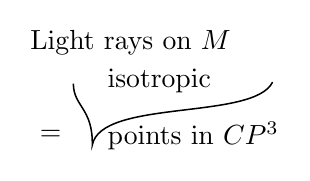
\begin{tikzpicture}[line width=.55pt,every node/.style={inner sep=1pt,anchor=west}]
\node at (0,1.18) {Light rays on \(M\)};
\node at (.12,0) {\(=\)};
\node at (.98,.69) {isotropic};
\draw (.59,.66) .. controls (.59,.37) and (.84,.35) .. (.83,-.12)
 .. controls (.94,.47) and (2.88,.19) .. (3.12,.68);
\node at (.98,0) {points in \(\mathbb{C}P^3\)};
\end{tikzpicture}}\endgroup}
\end{GelfandAdjacentEvidence}
\begin{GelfandAdjacentEvidence}{GELFAND-P000858}{7}


\uwave{Contest}: formulate a higher-dimensional generalization of this situation.
\SourceFigure{GELFAND-P000858}{flag-arrow}{%
\begingroup\color{black}\GelfandFitDiagram{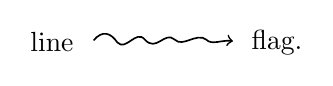
\begin{tikzpicture}[line width=.6pt,every node/.style={inner sep=1pt}]
\node[anchor=east] at (0,0) {line};
\draw[->] (.21,.015) .. controls (.32,.15) and (.43,.11) .. (.51,-.01)
 .. controls (.62,-.13) and (.75,.16) .. (.86,.025)
 .. controls (1.01,-.14) and (1.11,.14) .. (1.24,.025)
 .. controls (1.34,-.08) and (1.52,.12) .. (1.64,.025)
 .. controls (1.71,-.05) and (1.84,.025) .. (1.98,.005);
\node[anchor=west] at (2.17,-.015) {flag.};
\end{tikzpicture}}\endgroup}
\end{GelfandAdjacentEvidence}


\begin{center}— \(\cdot\) —\end{center}


\Needspace{7\baselineskip}
\SourcePage{GELFAND-P000859}{unlabelled}
\uuline{15.10.79.} \quad \uline{Gelfand Sem.}

\uuline{F. A. Berezin.} \quad \uline{Supermathematics.}

\(\mathbb K\) — a field (\(\mathbb R\) or \(\mathbb C\)).

\(\mathbb Z_2\)-graded space \(L=L_0\oplus L_1\).

The elements of \(L_0\) and \(L_1\) are called homogeneous.

Parity
\[
\alpha(x)=\begin{cases}
0,&x\in L_0\\
1,&x\in L_1.
\end{cases}
\]
Sums and prod. are taken \(\bmod 2\).

Grassm. algebra \(\Lambda\) over \(\mathbb K\) — assoc. alg. with generators
\[
1\ (\in\mathbb K),\quad \xi_1,\ldots,\xi_N
\]
and relat.
\[
\xi_i\xi_j+\xi_j\xi_i=0,\qquad \forall i,j.
\]
\[
\{1,\ \xi_{i_1}\ldots\xi_{i_k},\ i_1<i_2<\ldots<i_k\}
\quad\text{— a basis in }\Lambda\text{ over }\mathbb K.
\]
\(\Lambda=\Lambda_0\oplus\Lambda_1\), \quad
\(\Lambda_0\) is gen. by \(1\) and prod. of an even number of \(\xi_i\).


\Needspace{7\baselineskip}
\begin{GelfandAdjacentEvidence}{GELFAND-P000860}{1}
\SourcePage{GELFAND-P000860}{10}
\[
\dim_{\mathbb K}\Lambda=2^N.
\]
For homogeneous \(f,g\)
\[
f\cdot g=(-1)^{\alpha(f)\cdot\alpha(g)}gf.\tag{1}
\]
Grassmann envelope of the lin. space \(L\):

[crossed out: \sout{\((2)\quad L(\Lambda)=L\otimes_{\mathbb K}\Lambda\)}]
\Unclear{GELFAND-P000860}{cancelled-definition}{The hatched-out entry provisionally reads \((2)\quad L(\Lambda)=L\otimes_{\mathbb K}\Lambda\).}
\end{GelfandAdjacentEvidence}
\begin{GelfandAdjacentEvidence}{GELFAND-P000860}{2}


\(e_i\) — a basis in \(L\) of homog. elements
(\(L=L_0\oplus L_1\)).

Now consider
\[
\left\{\sum a_i e_i,\ a_i\in\Lambda,\ \alpha(a_i)=\alpha(e_i)\right\}
\underset{\mathrm{def}}{=}L(\Lambda).\tag{2}
\]
\uwave{This is a left \(\Lambda_0\)-module.} Equivalently:
\[
L(\Lambda)=\left(\Lambda\underset{\mathbb K}{\otimes}L\right)_{\bar 0}.
\tag*{\((2)'\)}
\]
Linear operators.

\uline{I.M.G.} These alg. arise in the theory of quiver repr. (cf. FA, 1979; \(N=3\)).

\uwave{Conj.}: \(\forall\) Dynkin diagram there should be an analogue of the \uwave{even part of the Grassm. algebra}.
(so that the ordinary one corresp. to the diagram \(A_n\)

\SourceFigure{GELFAND-P000860}{dynkin-chain}{%
\begingroup\color{black}\GelfandFitDiagram{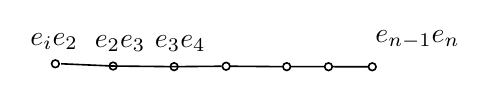
\begin{tikzpicture}[line width=.58pt,x=.52cm,y=.52cm,every node/.style={inner sep=1pt}]
\draw (.14,0)--(1.41,-.055)--(2.90,-.07)--(4.06,-.06);
\draw (4.27,-.06)--(5.54,-.07);
\draw (5.76,-.07)--(6.56,-.071);
\draw (6.78,-.071)--(7.63,-.073);
\foreach \x/\y in {0/0,1.41/-.055,2.90/-.07,4.17/-.06,5.65/-.07,6.67/-.071,7.74/-.073}
  \draw (\x,\y) circle (.093);
\node at (-.03,.54) {\(e_i e_2\)};
\node at (1.58,.50) {\(e_2e_3\)};
\node at (3.05,.50) {\(e_3e_4\)};
\node[anchor=west] at (7.73,.59) {\(e_{n-1}e_n\)};
\end{tikzpicture}}\endgroup\par
The dotted first subscript is read as \(i\). No arrowheads can be made out on the chain.}
\end{GelfandAdjacentEvidence}
\begin{GelfandAdjacentEvidence}{GELFAND-P000860}{3}


if joined by an arrow, then the prod. is \(=0\), if unjoined, then there is a new element.
Idea: there are other alg. of Grassmann type.
\begin{center}— \(\cdot\) —\end{center}

operator in \(L\):
\Unclear{GELFAND-P000860}{operator-intro}{There is a dark stroke at the right end of \(L\). A separate subscript cannot be established.}
\end{GelfandAdjacentEvidence}
\begin{GelfandAdjacentEvidence}{GELFAND-P000860}{4}

\[
A=\begin{pmatrix}A_{11}&A_{12}\\ A_{21}&A_{22}\end{pmatrix}.\tag{3}
\]
Grading:

[crossed out: \sout{…}]
\Incomplete{GELFAND-P000860}{grading-cancellation}{The sign before the first matrix is crossed out. It may be \(A\).}
\end{GelfandAdjacentEvidence}
\begin{GelfandAdjacentEvidence}{GELFAND-P000860}{5}

\SourceFigure{GELFAND-P000860}{grading-labels}{%
\begingroup\color{black}\GelfandFitDiagram{\begin{tikzpicture}[line width=.54pt,every node/.style={inner sep=1pt}]
\node at (-1.55,.10) {(4)};
\node (even) at (0,0) {\(\begin{pmatrix}A_{11}&0\\0&A_{22}\end{pmatrix}\)};
\node (odd) at (2.62,-.08) {\(\begin{pmatrix}0&A_{12}\\ A_{21}&0\end{pmatrix}\)};
\draw (-.23,-.80)--(-.23,-.99);
\draw (2.66,-.84)--(2.62,-1.02);
\node[anchor=west] at (-.46,-1.20) {0th comp.};
\node[anchor=west] at (2.33,-1.22) {1st comp.};
\end{tikzpicture}}\endgroup}
\end{GelfandAdjacentEvidence}
\begin{GelfandAdjacentEvidence}{GELFAND-P000860}{6}

\Unclear{GELFAND-P000860}{grading-matrix-odd}{The lower left block in the second matrix is read as \(A_{21}\).}
\end{GelfandAdjacentEvidence}
\begin{GelfandAdjacentEvidence}{GELFAND-P000860}{7}


The space \(L_{p,q}\) — all such oper., \(p=\dim L_0\), \(q=\dim L_1\).

\(L_{p,q}(\Lambda)\) — Grassm. envelope:

\uline{Remark}: \(a_i\) and \(e_i\) are always taken to commute.

\(L_{p,q}(\Lambda)\) — also matrices of Grassm. numbers:

in \(A_{11},A_{22}\) even
\Unclear{GELFAND-P000860}{even-block-indices}{The first pair of subscripts is heavily retraced and provisionally reads \(11\). The second reads \(22\).}
\end{GelfandAdjacentEvidence}


in \(A_{12},A_{21}\) odd.


\Needspace{7\baselineskip}
\begin{GelfandAdjacentEvidence}{GELFAND-P000861}{1}
\SourcePage{GELFAND-P000861}{unlabelled}
\[
A=\begin{pmatrix}A_{11}&A_{12}\\A_{21}&A_{22}\end{pmatrix}\in L_{p,q}(\Lambda).
\]
\(L_{p,q}(\Lambda)\) — \uline{is an algebra} (and a \(\Lambda_0\)-module).

Supertrace
\[
\operatorname{str} A=\operatorname{tr} A_{11}-\operatorname{tr} A_{22}.\tag{5}
\]
Prop.:
\[
\operatorname{str}(AB)=\operatorname{str}(BA)\tag{6}
\]
\uwave{Superdeterminant}. (Berezinian):
\[
\operatorname{sdet}=\det(A_{11}-A_{12}A_{22}^{-1}A_{21})(\det A_{22})^{-1}\tag{7}
\]
(for numerical matrices there is a fmla. [crossed out: \sout{…}] of the same form, but with
\(\det A_{22}\) in place of \((\det A_{22})^{-1}\)).
\Incomplete{GELFAND-P000861}{cancelled-word}{The entry after “fmla.” is crossed out and illegible.}
\end{GelfandAdjacentEvidence}
\begin{GelfandAdjacentEvidence}{GELFAND-P000861}{2}

\[
\operatorname{sdet}(\alpha_1\alpha_2)=
\operatorname{sdet}\alpha_1\cdot\operatorname{sdet}\alpha_2\tag{8}
\]
\Unclear{GELFAND-P000861}{product-symbols}{The symbols in (8) are provisionally set as \(\alpha_1,\alpha_2\). They could be cursive capitals \(A_1,A_2\).}
\end{GelfandAdjacentEvidence}
\begin{GelfandAdjacentEvidence}{GELFAND-P000861}{3}


\uline{Exercise}. Do this if \(\dim L_0=\dim L_1=1\), i.e. for matrices of order 2.

\uwave{Explanation}. Consider matrices with anticomm. entries:
\[
\operatorname{sdet}\begin{pmatrix}1&\xi_1\\\xi_2&1\end{pmatrix}
 =1-\xi_1\xi_2.
\]
\[
\begin{pmatrix}1&\xi_1\\\xi_2&1\end{pmatrix}^{2}
=\begin{pmatrix}1+\xi_1\xi_2&2\xi_1\\2\xi_2&1+\xi_2\xi_1\end{pmatrix}.
\]
\SourceFigure{GELFAND-P000861}{post-matrix-mark}{%
\begingroup\color{black}\GelfandFitDiagram{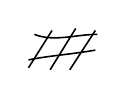
\begin{tikzpicture}[line width=.57pt,x=.025cm,y=-.025cm]
\draw (10,12) .. controls (20,16) and (31,12) .. (42,12);
\draw (7,25) .. controls (16,23) and (30,22) .. (41,20);
\draw (7,29)--(19,10);
\draw (18,30)--(31,9);
\draw (28,30)--(41,10);
\end{tikzpicture}}\endgroup\par
A small hash-like sign sits to the right of the matrix. Its purpose is unclear.}
\end{GelfandAdjacentEvidence}
\begin{GelfandAdjacentEvidence}{GELFAND-P000861}{4}

\[
\begin{aligned}
\operatorname{sdet}
 &=(1+\xi_1\xi_2-2\xi_1(1+\xi_1\xi_2)2\xi_2)(1+\xi_1\xi_2)=\\
 &=(1-3\xi_1\xi_2)(1+\xi_1\xi_2)=1-2\xi_1\xi_2=(1-\xi_1\xi_2)^2.
\end{aligned}
\]
\Unclear{GELFAND-P000861}{sdet-calc-first}{In the first product after \(1+\), the first subscript is retraced and read as \(1\).}
\end{GelfandAdjacentEvidence}
\begin{GelfandAdjacentEvidence}{GELFAND-P000861}{5}


\uwave{Reduction of matrices to canon. form.}

\(L(\Lambda)\)
\Unclear{GELFAND-P000861}{faded-fragment}{The separate faded entry is provisionally read as \(L(\Lambda)\).}
\end{GelfandAdjacentEvidence}
\begin{GelfandAdjacentEvidence}{GELFAND-P000861}{6}


There is a mapping
\[
m.\quad L(\Lambda)\longrightarrow L_0
\]
\[
\begin{aligned}
\sum a_i e_i
&\longmapsto\left.\left(\sum a_i e_i\right)\right|_{\xi=0}
=\sum_i m(a_i)e_i,\\
&m(a_i)=\left.a_i\right|_{\xi=0}.
\end{aligned}
\]
\Incomplete{GELFAND-P000861}{cancelled-sum-index}{The lower entry at the last summation is crossed out. An undeciphered stroke is visible above the sign.}
\end{GelfandAdjacentEvidence}
\begin{GelfandAdjacentEvidence}{GELFAND-P000861}{7}

\[
A=\begin{pmatrix}A_{11}&A_{12}\\A_{21}&A_{22}\end{pmatrix}\in L_{p,q}(\Lambda).
\]
\Unclear{GELFAND-P000861}{lower-matrix-space}{The stroke of \(L\) in the second matrix line is broken. The expression is provisionally read as \(L_{p,q}(\Lambda)\).}
\end{GelfandAdjacentEvidence}

\[
m(A)=\begin{pmatrix}a_1&0\\0&a_2\end{pmatrix}.\tag{9}
\]
Let \(\mathbb K=\mathbb C\).

\uline{Theorem}.

Let \(m(A)\) have distinct eigenv.. Then \(A\) also reduces to diag. form:
\[
BAB^{-1}=\begin{pmatrix}c_1&&0\\&\ddots&\\0&&c_{p+q}\end{pmatrix}.\tag{10}
\]


\Needspace{7\baselineskip}
\begin{GelfandAdjacentEvidence}{GELFAND-P000862}{1}
\SourcePage{GELFAND-P000862}{11}
\uwave{Analogues of Jordan blocks are unknown here.}

\uline{Problem 1}. \uwave{Do this} (\uwave{analogue of normal forms})!

A problem related to instantons:

\uline{Problem 2}. Consid. the matrix \(A=(a_{ik})_{i,k=1}^{n}\) with entries
\(a_{ik}\in\Lambda_1\) (odd Grassm. numbers).

Describe all \(B=(b_{ik})_{i,k=1}^{n}\), with entr. \(b_{ik}\in\Lambda_0\) such that
\[
\underline{\underline{AB=BA}}.
\]
If \(\Lambda\) has 4 generators, then it has a relation to Y.-M.
If all entr. of \(A\) are independent (in \(\Lambda\)), then it can be solved.
\begin{center}— \(\cdot\) —\end{center}

\uuline{S.G.} Connection with the work of Beilinson and Bernst.–Gelf.–Gelf.

(see FA, 1978, \(N=3\)?; or Drinfeld, Manin; Nucl. Physics, \(N=6\), 1979:
the constr. is given explicitly there, translated into the language of solutions).
\Unclear{GELFAND-P000862}{reference-issue}{The question mark after \(N=3\) is in the manuscript.}
\end{GelfandAdjacentEvidence}
\begin{GelfandAdjacentEvidence}{GELFAND-P000862}{2}


\uwave{classif. of vect. bundles} on \(\mathbb C P^3\). (holom.)

Objects — graded modules over \(\Lambda=\Lambda(4)\):
\SourceFigure{GELFAND-P000862}{graded-chain}{%
\begingroup\color{black}\GelfandFitDiagram{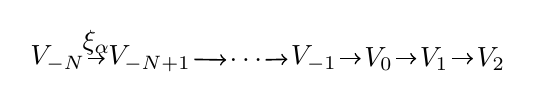
\begin{tikzpicture}[line width=.59pt,x=.72cm,y=.72cm,every node/.style={inner sep=1pt}]
\node (a) at (0,0) {\(V_{-N}\)};
\node (b) at (1.62,0) {\(V_{-N+1}\)};
\node (c) at (3.32,-.03) {\(\ldots\)};
\node (d) at (4.52,0) {\(V_{-1}\)};
\node (e) at (5.66,0) {\(V_0\)};
\node (f) at (6.64,0) {\(V_1\)};
\node (g) at (7.64,0) {\(V_2\)};
\draw[->] (a)--node[above] {\(\xi_\alpha\)} (b);
\draw[->] (b)--(c);
\draw[->] (c)--(d);
\draw[->] (d)--(e);
\draw[->] (e)--(f);
\draw[->] (f)--(g);
\end{tikzpicture}}\endgroup}
\end{GelfandAdjacentEvidence}
\begin{GelfandAdjacentEvidence}{GELFAND-P000862}{3}

\(\alpha=1,2,3,4\). \quad Repr. of the Grassm. algebra:
\[
\xi_i\xi_j+\xi_j\xi_i=0.
\]
\(a_1\xi_1+a_2\xi_2+a_3\xi_3+a_4\xi_4\) — an operator from \(V_k\) to \(V_{k+1}\)

and we get a \uline{complex};

the cohom. vanish except for \(H^0\).

Such modules up to triv. classify instantons.
\Unclear{GELFAND-P000862}{module-equivalence}{The abbreviation after “up to” provisionally reads «трив.» (“triv.”).}
\end{GelfandAdjacentEvidence}
\begin{GelfandAdjacentEvidence}{GELFAND-P000862}{4}


\dashuline{Problem}: give an explicit construction. It has yet to be done (the spaces are constructed, but the mappings are missing).

\dashuline{Problem}: \uwave{give the classif. for the Grassmannian}!!

\uuline{Yu. Shabat.}
\Unclear{GELFAND-P000862}{speaker-initial}{The manuscript gives the initial «Ю.» (“Yu.”). \href{https://old.mccme.ru/gelfand/notes/record-469.html}{MCCME catalogue record 469} gives the name as “G.B. Shabat”.}
\end{GelfandAdjacentEvidence}
\begin{GelfandAdjacentEvidence}{GELFAND-P000862}{5}


\uline{Lie–Wirtinger theorem} (classical)

\(\Gamma\subset\mathbb C^n\) — a germ of an analytic hypersurface.
It is called a \uwave{double translation surf.}, if it can be represented in 2 ways as a sum
\[
\Gamma=\gamma_1+\ldots+\gamma_{n-1},
\qquad
\Gamma=\delta_1+\ldots+\delta_{n-1}
\]
\(\gamma_i,\delta_i\) — germs of analytic curves.

\(\{\gamma_i\}\) and \(\{\delta_i\}\) cannot be obtained from one another by perm.
[crossed out: \sout{…}] and translations.
\Incomplete{GELFAND-P000862}{cancelled-qualifier}{The entry after “perm.” is crossed out and illegible.}
\end{GelfandAdjacentEvidence}


\uline{Example}: \(X\) — a smooth curve of genus \(n\).

\(JX\) — the Jacobian of the curve \(X\); \quad \(j:X\longrightarrow JX\).


\Needspace{7\baselineskip}
\begin{GelfandAdjacentEvidence}{GELFAND-P000863}{1}
\SourcePage{GELFAND-P000863}{unlabelled}
\[
\Theta=\underbrace{j(X)+\ldots+j(X)}_{n-1\text{ times}},
\qquad (\Theta\text{ — Poincaré divisor}).
\]
By Riemann’s thm. it is symm., i.e. \(\exists K\in JX\):
\[
\Theta=K-\Theta.
\]
\Unclear{GELFAND-P000863}{riemann-constant}{The sign is set as \(K\) in both places. Another possible reading is \(\kappa\).}
\end{GelfandAdjacentEvidence}
\begin{GelfandAdjacentEvidence}{GELFAND-P000863}{2}


Therefore up to translation
\[
\Theta\sim\underbrace{-jX-\ldots-jX}_{n-1}.
\]
Let \(X\ne-jX\) (\(\Leftrightarrow X\) is nonhyperelliptic).
\Unclear{GELFAND-P000863}{embedded-curve}{The manuscript has \(X\) on the left with no preceding \(j\).}
\end{GelfandAdjacentEvidence}
\begin{GelfandAdjacentEvidence}{GELFAND-P000863}{3}


\uline{Assertion}: all translation surf. are these surf. and their degenerations

(if \(\Gamma\) — a double translation surf., then a small deform. of \(\Gamma\) — a germ of \(\Theta\subset JX\)).

\uline{Conjecture of I.M.G.}: 1) All integr. systems have this theorem as their basis.

2) This thm. is the first in a series of coloss. theorems of this kind.
\Unclear{GELFAND-P000863}{hypothesis-word}{The abbreviation «колосал.» is a provisional reading. The middle strokes run together.}
\end{GelfandAdjacentEvidence}
\begin{GelfandAdjacentEvidence}{GELFAND-P000863}{4}


1) — the reason for the appearance of \(\Theta\)-funcs..
\begin{center}— \(\cdot\) —\end{center}

\uuline{Höegh-Krohn?} \quad \uuline{someone from Norway.} (interpreted by Gelfand).
\Unclear{GELFAND-P000863}{speaker-name}{The manuscript puts a question mark after the name. \href{https://old.mccme.ru/gelfand/notes/record-470.html}{MCCME catalogue record 470} gives “Raphael Hoegh-Krohn”.}
\end{GelfandAdjacentEvidence}
\begin{GelfandAdjacentEvidence}{GELFAND-P000863}{5}


On mapping grps.

(Ismagilov, Graev, Vershik; Albeverio)

[below the list: and \ldots]

\(X\) — a Riem. manifold

\(G\) — a compact Lie gr. (simple)
\[
\varphi\in C_0^\infty(X,G)\equiv G^X.
\]
\Unclear{GELFAND-P000863}{mapping-letter}{The open-loop sign is provisionally set as \(\varphi\). Another possible reading is \(\psi\).}
\end{GelfandAdjacentEvidence}
\begin{GelfandAdjacentEvidence}{GELFAND-P000863}{6}

We study unit. representations.

\(g\) — the Lie alg. of \(G\).

[crossed out at left: \sout{…}] \(\Omega(X,g)\) — 1-forms with values in the Lie alg..
\Incomplete{GELFAND-P000863}{cancelled-form-prefix}{The sign before \(\Omega(X,g)\) is crossed out and illegible.}
\end{GelfandAdjacentEvidence}
\begin{GelfandAdjacentEvidence}{GELFAND-P000863}{7}

\[
\omega_i\in\Omega(X,g)
\]
\[
(\omega_1,\omega_2)=\int_X\operatorname{tr}\bigl(\omega_1(x)\omega_2^*(x)\bigr)\,dx.\tag{1}
\]
\Unclear{GELFAND-P000863}{cancelled-star}{The dark stroke above \(\omega_1\) may be a crossed-out star. Its reading is uncertain.}
\end{GelfandAdjacentEvidence}
\begin{GelfandAdjacentEvidence}{GELFAND-P000863}{8}

\[
\omega_i(x):T_x\longrightarrow g
\]
there is an inner prod. in both spaces (on the right, Killing)

\SourceFigure{GELFAND-P000863}{adjoint-identification}{%
\begingroup\color{black}\GelfandFitDiagram{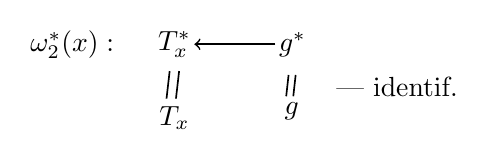
\begin{tikzpicture}[line width=.6pt,every node/.style={inner sep=1pt}]
\node[anchor=east] at (-.72,.72) {\(\omega_2^*(x):\)};
\node (txdual) at (0,.72) {\(T_x^*\)};
\node (gdual) at (1.50,.72) {\(g^*\)};
\draw[->] (gdual.west)--(txdual.east);
\draw (-.06,.38)--(-.10,.03) (.06,.38)--(.02,.03);
\draw (1.45,.33)--(1.42,.06) (1.54,.33)--(1.51,.06);
\node at (0,-.22) {\(T_x\)};
\node at (1.49,-.13) {\(g\)};
\node[anchor=west] at (2.01,.18) {— identif.};
\end{tikzpicture}}\endgroup}
\end{GelfandAdjacentEvidence}



\Needspace{7\baselineskip}
\begin{GelfandAdjacentEvidence}{GELFAND-P000864}{1}
\SourcePage{GELFAND-P000864}{12}
\[
\omega_1\omega_2^*:g\longrightarrow g
\]
the trace and the integr. can now be taken

\(\mathcal H\) — a Hilbert sp., completion of \(\Omega(X,g)\)
\[
L_2(\mathcal H,\mu)
\]
\[
\dim\mathcal H<\infty\quad\Rightarrow\quad d\mu\sim e^{-\frac12|x|^2}\,dx
\]
\Unclear{GELFAND-P000864}{finite-dimension-sign}{The \(\infty\) sign is retraced. A separate stroke is visible beneath it.}
\end{GelfandAdjacentEvidence}
\begin{GelfandAdjacentEvidence}{GELFAND-P000864}{2}

(and analog. in an [crossed out: \sout{finite}] \(\infty\)-dim. sp.)
\Unclear{GELFAND-P000864}{cancelled-word}{The crossed-out word provisionally reads «конечно» (“finite”).}
\end{GelfandAdjacentEvidence}
\begin{GelfandAdjacentEvidence}{GELFAND-P000864}{3}


\(T\in E(\mathcal H)\) — Euclidean transf. (motions) of the space \(\mathcal H\),
\[
Tx=Ox+a,\qquad x\in H,\quad a\in H
\]
\(\mu\) is inv. under \(O\) and quasi-inv. under translations.

\(g\in E(\mathcal H)\), \(g\to U_g\) unitary on \(L_2(\mathcal H,\mu)\)

hence [«ср.»] a unit. repr. of \(E(\mathcal H)\) in \(L_2(\mathcal H,\mu)\)
\Unclear{GELFAND-P000864}{representation-abbrev}{The abbreviation is provisionally read «ср.». The second sign has a long descending stroke.}
\end{GelfandAdjacentEvidence}
\begin{GelfandAdjacentEvidence}{GELFAND-P000864}{4}

\[
(\alpha(\varphi)\omega)(x)=\operatorname{Ad}\varphi(x)\,\omega(x)
+\varphi^{-1}(x)\,d\varphi(x).\tag{2}
\]
\Unclear{GELFAND-P000864}{mapping-letter}{The open-loop sign is provisionally set as \(\varphi\). Another possible reading is \(\psi\).}
\end{GelfandAdjacentEvidence}
\begin{GelfandAdjacentEvidence}{GELFAND-P000864}{5}

\Unclear{GELFAND-P000864}{affine-law}{The manuscript shows the order \(\varphi^{-1}(x)\,d\varphi(x)\) and the exponent \(-1\).}
\end{GelfandAdjacentEvidence}
\begin{GelfandAdjacentEvidence}{GELFAND-P000864}{6}

\[
\alpha:C_0^\infty(X,G)\longrightarrow E(\Omega(X))
\]
— this is a group homomorphism:
\[
\alpha(\varphi_1\varphi_2)=\alpha(\varphi_1)\alpha(\varphi_2).
\]
Take the comp. with \(U_g\);
\[
\underline{\underline{V_\phi=U_{\alpha(\phi)}}}
\quad\text{— we get a unit. repr.}
\]
\Unclear{GELFAND-P000864}{boxed-map-letters}{The loops in the underlined equation have a different shape. They are set here as \(\phi\).}
\end{GelfandAdjacentEvidence}

\[
\varphi\longrightarrow V_\varphi.
\]
\uline{Theorem 1}. It is irreducible if \(\dim X\geq 3\).
\[
\begin{aligned}
\geq5&\text{ — Ismagilov}\\
\geq4&\text{ — Gelf., Graev, Vershik}\\
\geq3&\text{ — Albeverio and Høegh-Krohn.}
\end{aligned}
\]
\uline{Theorem 2}. \(\dim X=1\quad\Rightarrow\) the repr. is reducible
\[
\underline{\dim X=2}\qquad\text{— ?}
\]
\(b(t)\) — Brownian mot. in \(g\). (standard; with resp. to the Killing form)

Consid. the eq.
\[
\eta^{-1}(t)\,d\eta(t)=db(t),\qquad
\eta\in C(\mathbb R^+,G).\tag{3}
\]


\Needspace{7\baselineskip}
\begin{GelfandAdjacentEvidence}{GELFAND-P000865}{1}
\SourcePage{GELFAND-P000865}{unlabelled}
Explanation:

\(b(t)\) — a measure on \(C_0(\mathbb R^+,g)\) — denote it by \(\mu_0\).
\[
b(t)\in\bigl(C_0(\mathbb R^+,g),\mu\bigr)
\]
Solve the ordinary eq.
 
We obtain the map
\[
\bigl(C(\mathbb R^+,G),\mu_0\bigr)\longrightarrow C(\mathbb R^+,G)
\]
\Unclear{GELFAND-P000865}{path-measure-notation}{The first formula has \(C_0(\mathbb R^+,g)\) with \(\mu\). The domain of the map has \(C(\mathbb R^+,G)\) with \(\mu_0\).}
\end{GelfandAdjacentEvidence}
\begin{GelfandAdjacentEvidence}{GELFAND-P000865}{2}


Stochastic — solve and transfer the measure.
\[
\eta(t)\longrightarrow\phi(t)\eta(t);
\]
\Unclear{GELFAND-P000865}{mapping-letter}{The closed-loop letter in these two formulas is provisionally set as \(\phi\).}
\end{GelfandAdjacentEvidence}
\begin{GelfandAdjacentEvidence}{GELFAND-P000865}{3}

\[
\frac{d\mu(\phi\eta)}{d\mu(\eta)}
\]
\SourceFigure{GELFAND-P000865}{nationality-insertions}{%
\begingroup\color{black}\GelfandFitDiagram{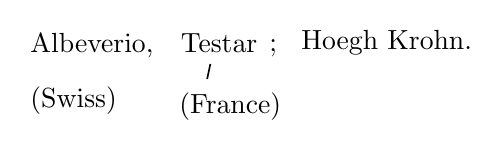
\begin{tikzpicture}[line width=.59pt,every node/.style={inner sep=1pt}]
\node[anchor=west] at (0,.63) {Albeverio,};
\node[anchor=west] at (1.91,.65) {Testar};
\node at (3.13,.59) {;};
\node[anchor=west] at (3.44,.66) {Hoegh Krohn.};
\node[anchor=west] at (0,-.07) {(Swiss)};
\draw (2.33,.39)--(2.29,.20);
\node[anchor=west] at (1.89,-.15) {(France)};
\end{tikzpicture}}\endgroup}
\end{GelfandAdjacentEvidence}
\begin{GelfandAdjacentEvidence}{GELFAND-P000865}{4}

\Unclear{GELFAND-P000865}{latin-name}{The first name is provisionally read as “Albeverio”. The second reads “Testar”. In the later \href{https://doi.org/10.1016/0022-1236(81)90082-3}{1981 article} the names are printed as S. Albeverio, R. Høegh-Krohn and D. Testard.}
\end{GelfandAdjacentEvidence}
\begin{GelfandAdjacentEvidence}{GELFAND-P000865}{5}

\[
L_2\bigl(C(\mathbb R^+,G),\mu\bigr),\qquad
\varphi\in C^\infty(\mathbb R^+,G)
\]
\Unclear{GELFAND-P000865}{mapping-letter-open}{The open loop in the line with \(C^\infty\) is set as \(\varphi\).}
\end{GelfandAdjacentEvidence}

\[
\eta\longrightarrow\varphi\eta
\]
\(\varphi\longrightarrow W_\varphi\) \quad we get a unit. repr. on \(L_2(C(\mathbb R^+,G),\mu)\)

\uline{Theorem} \(W_\varphi\cong V_\varphi\) \quad equivalent.

The corresp. cocycle — the Maurer–Cartan form.

Factors:
\[
[L_\infty\cup W_\varphi]''\qquad\text{— a factor of type 3.}
\]


\Needspace{7\baselineskip}
\begin{GelfandAdjacentEvidence}{GELFAND-P000866}{1}
\SourcePage{GELFAND-P000866}{unlabelled}
\uuline{22.10.79} \qquad \uuline{Gelfand Sem.}

\uline{Someone.} (\uuline{Baturin})
\Unclear{GELFAND-P000866}{speaker-name}{The handwritten name is provisionally read «Батурин» (“Baturin”). \href{https://old.mccme.ru/gelfand/notes/record-471.html}{MCCME catalogue record 471} gives “I.A. Batalin”.}
\end{GelfandAdjacentEvidence}
\begin{GelfandAdjacentEvidence}{GELFAND-P000866}{2}


\uline{On constraints.}

\uwave{First-class constraints}
\[
\begin{aligned}
H&\text{ — Hamiltonian},\qquad T_\alpha\text{ — constraints}\\
H,T_\alpha&\text{ — funcs. of }q\text{ and }p.
\end{aligned}\tag{1}
\]
\[
\{T_\alpha,T_\beta\}=u_{\alpha\beta}^{\gamma}T,\qquad
g^a=\begin{pmatrix}q^i\\p_i\end{pmatrix}.\tag{2}
\]
\Unclear{GELFAND-P000866}{constraint-index}{No subscript is visible on \(T\) after \(u_{\alpha\beta}^{\gamma}\).}
\end{GelfandAdjacentEvidence}
\begin{GelfandAdjacentEvidence}{GELFAND-P000866}{3}

\[
\{A,B\}=\frac{\partial A}{\partial g^a}\,\varepsilon^{ab}
\frac{\partial B}{\partial g^b},\qquad
\text{here }-\varepsilon^{ba}=\varepsilon^{ab}
=\begin{pmatrix}0&1\\-1&0\end{pmatrix}.\tag{3}
\]
First-class constraints — if condition (2) is satisfied, \quad
\(u_{\alpha\beta}^{\gamma}=u_{\alpha\beta}^{\gamma}(p,q)\).
\[
\text{\uline{Question}:}\quad
\text{can changes of var. be made so that}\quad u_{\alpha\beta}^{\gamma}=\mathrm{const}.\tag{4}
\]
\uline{Rem. on the motivation}: gauge transf. are gener. only by first-class constraints

\uwave{Action}:
\[
S=\int dt\left[\frac12 g^a\varepsilon_{ab}\dot g^b-H-\lambda^\alpha T_\alpha\right].\tag{5}
\]
(\(\lambda^\alpha\) — ordinary variables;
[crossed out: \sout{…}] the extremum is now unconstrained)
\Incomplete{GELFAND-P000866}{cancelled-extremum}{The entry before “the extremum” is crossed out and illegible.}
\end{GelfandAdjacentEvidence}
\begin{GelfandAdjacentEvidence}{GELFAND-P000866}{4}


Gauge transf. are gener. by the constraints
 
[crossed out below: \sout{\(g^a\quad\delta g^a=\cdots\)}]
\Unclear{GELFAND-P000866}{cancelled-coordinate}{The strokes under the hatching provisionally read \(g^a\) and \(\delta g^a=\). The ending is illegible.}
\end{GelfandAdjacentEvidence}
\begin{GelfandAdjacentEvidence}{GELFAND-P000866}{5}

\begin{center}— \(\bullet\) —\end{center}

\uuline{R. Kallosh.} \qquad \uline{Quantum field theory}

[line crossed out: \sout{\((1)\quad\Delta\phi_l=\lambda_l\phi_l,\ \ldots\)}]
\Unclear{GELFAND-P000866}{cancelled-eigen-equation}{The left part of the crossed-out line provisionally reads \((1)\quad\Delta\phi_l=\lambda_l\phi_l\). The subscripts are indistinct.}
\end{GelfandAdjacentEvidence}
\begin{GelfandAdjacentEvidence}{GELFAND-P000866}{6}

\Incomplete{GELFAND-P000866}{cancelled-equation-right}{The right part after the comma is heavily hatched and illegible.}
\end{GelfandAdjacentEvidence}
\begin{GelfandAdjacentEvidence}{GELFAND-P000866}{7}


\uwave{New Nobel laureates}
\SourceFigure{GELFAND-P000866}{weak-interactions}{%
\begingroup\color{black}\GelfandFitDiagram{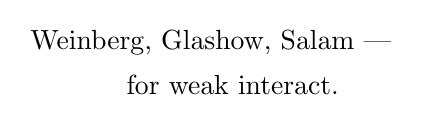
\begin{tikzpicture}[every node/.style={inner sep=1pt,anchor=west}]
\node at (0,.52) {\uwave{Weinberg, Glashow, Salam} —};
\node at (1.22,-.01) {for weak interact.};
\end{tikzpicture}}\endgroup}
\end{GelfandAdjacentEvidence}
\begin{GelfandAdjacentEvidence}{GELFAND-P000866}{8}


Symmetry underlies everything. Consid. the cont. integral.
\[
e^{iW[\varphi]}=\int d\phi\cdot\exp\{iS[\phi,\varphi]\}.\tag{1}
\]
\Unclear{GELFAND-P000866}{field-letter}{The open loop is set as \(\varphi\) (possibly \(\psi\)). The closed loop of the integration variable is set as \(\phi\).}
\end{GelfandAdjacentEvidence}
\begin{GelfandAdjacentEvidence}{GELFAND-P000866}{9}

\Incomplete{GELFAND-P000866}{cancelled-action-index}{The sign beneath \(S\) is blackened and illegible.}
\end{GelfandAdjacentEvidence}
\begin{GelfandAdjacentEvidence}{GELFAND-P000866}{10}


\(S\) is constructed from the class. action

from (1) much is determ.: probabilities, \(S\)-matrix.
\Unclear{GELFAND-P000866}{scattering-term}{The last letter in «матрице» (“matrix”) provisionally reads «е».}
\end{GelfandAdjacentEvidence}
\begin{GelfandAdjacentEvidence}{GELFAND-P000866}{11}


\(\phi\) — quantum fluct. (one averages over them)

\(S\)-matrix
\[
S[\varphi_{in}]=e^{iW[\widetilde{\varphi}[\varphi_{in}]]},\tag{2}
\]
\SourceFigure{GELFAND-P000866}{scattering-insertion}{%
\begingroup\color{black}\GelfandFitDiagram{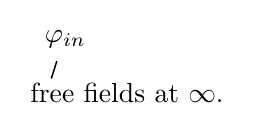
\begin{tikzpicture}[line width=.55pt,every node/.style={inner sep=1pt}]
\node at (0,.70) {\(\varphi_{in}\)};
\draw (-.11,.42)--(-.18,.20);
\node[anchor=west] at (-.49,.02) {free fields at \(\infty\).};
\end{tikzpicture}}\endgroup}
\end{GelfandAdjacentEvidence}



\Needspace{7\baselineskip}
\begin{GelfandAdjacentEvidence}{GELFAND-P000867}{1}
\SourcePage{GELFAND-P000867}{unlabelled}
\begin{equation*}
\widetilde{\varphi}=\varphi_{in}
+\int D^c(x-x')\frac{\delta\mathcal{L}_{int}}{\delta\widetilde{\varphi}(x')}\,d^4x'. \tag{3}
\end{equation*}
\Unclear{GELFAND-P000867}{field-letter}{The looped sign in (3) and in the diagram is read as $\varphi$ (possibly $\psi$).}
\end{GelfandAdjacentEvidence}
\begin{GelfandAdjacentEvidence}{GELFAND-P000867}{2}


(Yang--Feldman eq.)

Iterative sol. of (3) gives trees.

$D^c$ --- Green's fn. for the free Klein--Gordon eq.

\SourceFigure{GELFAND-P000867}{tree-diagram}{%
\begingroup\color{black}\GelfandFitDiagram{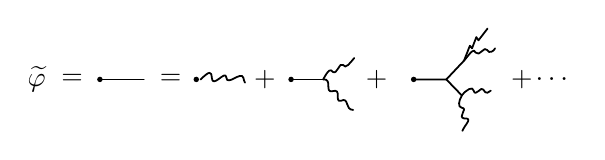
\begin{tikzpicture}[x=.68cm,y=.68cm,line width=.64pt,line cap=round,line join=round]
\node[inner sep=0pt] at (0,0) {$\widetilde{\varphi}$};
\node at (.66,0) {$=$};
\foreach \x in {1.18,2.98,4.75,7.04}
  \fill (\x,0) circle (.051);
\draw (1.18,0)--(2.00,0);
\node at (2.50,0) {$=$};
\draw (3.06,0)
  .. controls (3.23,.16) and (3.26,.16) .. (3.27,.03)
  .. controls (3.28,-.18) and (3.53,.19) .. (3.54,.04)
  .. controls (3.55,-.14) and (3.82,.17) .. (3.86,.03)
  .. controls (3.87,.00) and (3.87,-.04) .. (3.89,-.06);
\node at (4.26,0) {$+$};
\draw (4.75,0)--(5.35,0);
\draw (5.35,0)
  .. controls (5.45,.19) and (5.49,.20) .. (5.53,.14)
  .. controls (5.61,.08) and (5.66,.34) .. (5.72,.27)
  .. controls (5.77,.18) and (5.86,.32) .. (5.93,.40);
\draw (5.35,0)
  .. controls (5.53,.02) and (5.37,-.25) .. (5.52,-.22)
  .. controls (5.71,-.16) and (5.55,-.43) .. (5.68,-.40)
  .. controls (5.84,-.32) and (5.75,-.57) .. (5.91,-.57);
\node at (6.35,0) {$+$};
\draw (7.04,0)--(7.65,0)--(7.98,.35);
\draw (7.65,0)--(7.94,-.30);
\draw (7.98,.35)--(8.09,.63)--(8.13,.58)--(8.21,.79)
  --(8.25,.73)--(8.42,.95);
\draw (7.98,.35)
  .. controls (8.10,.49) and (8.16,.60) .. (8.20,.50)
  .. controls (8.26,.41) and (8.37,.64) .. (8.41,.55)
  .. controls (8.45,.47) and (8.54,.53) .. (8.56,.58);
\draw (7.94,-.30)
  .. controls (8.02,-.19) and (8.15,-.12) .. (8.16,-.21)
  .. controls (8.19,-.34) and (8.31,-.11) .. (8.34,-.19)
  .. controls (8.39,-.29) and (8.45,-.24) .. (8.48,-.21);
\draw (7.94,-.30)
  .. controls (7.88,-.40) and (7.86,-.52) .. (7.94,-.53)
  .. controls (8.07,-.54) and (7.84,-.71) .. (7.99,-.73)
  .. controls (8.15,-.72) and (8.00,-.84) .. (7.95,-.96);
\node at (9.06,0) {$+$};
\node at (9.62,0) {$\ldots$};
\end{tikzpicture}}\endgroup}
\end{GelfandAdjacentEvidence}
\begin{GelfandAdjacentEvidence}{GELFAND-P000867}{3}


Formula (2) contains amplitudes for prod. of any number of particles.

For gravity

\Unclear{GELFAND-P000867}{cancelled-action-sign}{A sign, possibly $\mathcal L$, is cancelled before $S_{\text{кл}}$.}
\end{GelfandAdjacentEvidence}
\begin{GelfandAdjacentEvidence}{GELFAND-P000867}{4}

\begin{equation*}
S_{\text{кл}}=\int\mathcal{L}\,d^4x,\qquad
\mathcal{L}=\sqrt{g}\,R[g_{\mu\nu}]. \tag{4}
\end{equation*}

$S$ in (1) differs by quantum corrections
\begin{equation*}
\begin{array}{cc}
\varphi&g_{\mu\nu}\\
\phi&h_{\mu\nu}
\end{array} \tag{5}
\end{equation*}
\Unclear{GELFAND-P000867}{field-pair}{The upper sign is read as $\varphi$ (possibly $\psi$), and the lower is rendered as $\phi$.}
\end{GelfandAdjacentEvidence}
\begin{GelfandAdjacentEvidence}{GELFAND-P000867}{5}

For gravity.
\begin{equation*}
e^{iW[g_{\mu\nu}]}=\int dh\cdot
 e^{i\{S_{\text{кл}}[g_{\mu\nu}+h_{\mu\nu}]+S_{\text{кал}}+S_{\text{ф.ч.}}\}}\,
 d\bar c\,dc. \tag{6}
\end{equation*}

ф. ч. --- \uwave{fictitious particles}.

$S_{\text{кл}}$ is given by formula (4) and is a functional of the metric $g$.

$h_{\mu\nu}$ --- \uwave{metric fluctuations}.
\begin{equation*}
S_{\text{кал.}}=\int\frac12
\left(D_\mu[g]h^{\mu}_{\nu}-\frac12 D_\nu[g]h_{\mu}^{\mu}\right)^2
\sqrt{g}\,d^4x. \tag{7}
\end{equation*}
\Unclear{GELFAND-P000867}{gauge-action-index}{The argument of the second $D$ runs into the beginning of $h$ and is read as $[g]$.}
\end{GelfandAdjacentEvidence}
\begin{GelfandAdjacentEvidence}{GELFAND-P000867}{6}


$D_\mu$ --- covariant deriv. for metric $g$

Raise and lower indices using $g$.
\begin{equation*}
S_{\text{ф.ч.}}=\int\sqrt{g}\,\bar c^{\nu}D_\mu[g]D^{\mu}[g+h]c_\nu\,d^4x. \tag{8}
\end{equation*}

$S_{\text{ф.ч.}}$ is constructed from $S_{\text{кал}}$ so that the answer does not depend on $S_{\text{кал}}$

(principle of quantum relativity).

\uwave{Observed by} \underline{Feynman}: without $S_{\text{кал}}$ there is no \textcolor{orange!65!black}{[cancelled]} unitarity (total prob. $=1$)
\Unclear{GELFAND-P000867}{cancelled-unitarity}{The short cancellation before “unitarity” is illegible.}
\end{GelfandAdjacentEvidence}
\begin{GelfandAdjacentEvidence}{GELFAND-P000867}{7}

\EvidenceBlock{GELFAND-P000867}{feynman-action-index}{The manuscript remark reads $S_{\text{кал}}$.}{\GelfandExcerptCaption}

He [did so] in 1st approx.

De Witt, Popov, Faddeev --- further.

\Unclear{GELFAND-P000867}{cancelled-bottom}{Cancelled Russian text: “В … зад”. The middle abbreviation is illegible, possibly “прибл.” (approx.).}
\end{GelfandAdjacentEvidence}


In supergrav. one further term suffices.


\Needspace{7\baselineskip}
\begin{GelfandAdjacentEvidence}{GELFAND-P000868}{1}
\SourcePage{GELFAND-P000868}{26}
In an arbitrary theory --- infinitely many terms.

\begin{equation*}
\underset{\text{(Einst.)}}{S_{\text{кл}}[g]}
\qquad\text{inv. under transformations}
\tag{9}
\end{equation*}
\begin{equation*}
\delta g_{\mu\nu}=D_\mu\xi_\nu+D_\nu\xi_\mu,\qquad
\xi_\mu\quad
\begin{array}{@{}l@{}}
\text{--- arbitrary vector}\\[-.25ex]
\text{\phantom{--- }(local fn. of $x$).}
\end{array}
\tag{10}
\end{equation*}

The quantum problem has an invariance:
\begin{equation*}
W[g_{\mu\nu}]=W[g_{\mu\nu}+\delta g_{\mu\nu}],\qquad
\delta g_{\mu\nu}\text{ taken from (10)}
\tag{11}
\end{equation*}

In fact (6) needs further specification.

Another invariance law. Consider:
\begin{equation*}
\begin{aligned}
e^{iW_{\text{рад}}}\underset{\mathrm{def}}{=}\int dh\cdot\exp i\Bigl\{
&S_{\text{кл}}[g+h]-S_{\text{кл}}[g]
-\frac{\delta S[g]}{\delta g_{\mu\nu}}h_{\mu\nu}+{}\\
&{}+S_{\text{кал}}\bigl(F(h)\bigr)+S_{\text{ф.ч.}}\bigl(F(h)\bigr)\Bigr\}.
\end{aligned}
\tag{12}
\end{equation*}
\Unclear{GELFAND-P000868}{eq12-final}{The stroke before $h$ has been retraced. The last argument is read as $F(h)$, possibly $Fh$.}
\end{GelfandAdjacentEvidence}
\begin{GelfandAdjacentEvidence}{GELFAND-P000868}{2}


$F$ --- a certain function satisfying certain conditions.

Gauge transf. [cancelled] preserve things with phys. meaning.
\Unclear{GELFAND-P000868}{text-cancel}{The cancelled word is illegible.}
\end{GelfandAdjacentEvidence}
\begin{GelfandAdjacentEvidence}{GELFAND-P000868}{3}


(The space remains \uwave{isometric} \uuline{to the old one}; same space, but I change the coord.).

\uwave{Adding the terms} $S_{\text{кал}},\ S_{\text{ф.ч.}}$
is needed to handle degen. in the stationary-phase expansion.

\begin{equation*}
W_{\text{рад}}[g_{\mu\nu}]_F
=W_{F+\delta F}[g]-\frac{\delta S[g]}{\delta g_{\mu\nu}}
\langle\delta h_{\mu\nu}\rangle
\tag{13}
\end{equation*}

$S_{\text{кал}}$ is added for convergence (correcting the degeneracy)
\[
\frac{\delta S}{\delta g_{\mu\nu}(x)\,\delta g_{\mu'\nu'}(x')}
\]
\Unclear{GELFAND-P000868}{derivative}{The numerator shows $\delta S$. No power on $\delta$ is discernible.}
\end{GelfandAdjacentEvidence}
\begin{GelfandAdjacentEvidence}{GELFAND-P000868}{4}


Form of the terms that can be added:
\begin{equation*}
S[\Phi]+\phi^i F_{i\alpha}\gamma^{\alpha\beta}F_{j\beta}\phi^j
\tag{14}
\end{equation*}
\Unclear{GELFAND-P000868}{fields-in-quadratic}{The two lowercase signs have two loops and are rendered as $\phi$, as is the lower sign in (5).}
\end{GelfandAdjacentEvidence}
\begin{GelfandAdjacentEvidence}{GELFAND-P000868}{5}


Let the external metric be flat
\begin{equation*}
S[\Phi]+\frac12\Phi^i F_{ij}\Phi^j
\tag{15}
\end{equation*}
\Unclear{GELFAND-P000868}{cancelled-formula}{Cancelled line, read as $S[g+h]+\sum\frac12\int h^{\mu\nu}(x)$. A cancellation stroke crosses the sign that resembles $\sum$.}
\end{GelfandAdjacentEvidence}



\Needspace{7\baselineskip}
\begin{GelfandAdjacentEvidence}{GELFAND-P000869}{1}
\SourcePage{GELFAND-P000869}{unlabelled}
\begin{equation*}
S[g+h]+\frac12\int h^{\mu\nu}(x)
F_{\mu\nu\mu'\nu'}(x,x',g)h^{\mu'\nu'}(x')\,d^4x\,d^4x'
\tag{16}
\end{equation*}
$F$ --- a sufficiently arbitrary fn. of the points and the metric, for example:
\begin{equation*}
\frac12\left(D_\mu h^\mu_\nu-\frac\beta2D_\nu h\right)^2
\qquad\text{or}\qquad h^\mu h_\mu^\nu
\tag{17}
\end{equation*}
\Unclear{GELFAND-P000869}{eq17-alt}{After “or” the manuscript gives $h^\mu h_\mu^\nu$. No lower index on the first $h$ is visible.}
\end{GelfandAdjacentEvidence}
\begin{GelfandAdjacentEvidence}{GELFAND-P000869}{2}


Principle of relativity --- it is independent of $F$. The result is a quadratic form
\begin{equation*}
\frac12\frac{\delta^2S[g+h]}{\delta h_{\mu\nu}(x)\,\delta h_{\mu'\nu'}(x')}
+F_{\mu\nu\mu'\nu'}(x,x')
\tag{18}
\end{equation*}
The quadratic form must be nondegenerate. This is a condition on $F$.

The addition in (16) is the gauge-fixing action.

\uwave{Read}: Faddeev, Popov --- review in UFN.

\Unclear{GELFAND-P000869}{cancelled-before13}{Two cancelled entries. The first may read “Теперь” (now). The lower one is illegible.}
\end{GelfandAdjacentEvidence}
\begin{GelfandAdjacentEvidence}{GELFAND-P000869}{3}

In (13):

$\langle\delta h_{\mu\nu}\rangle$ --- the change in the integral brought about by the given change of gauge.
\[
\langle\delta h_{\mu\nu}\rangle=\int dh\cdot\exp i\{\widetilde S\}
\]
\Unclear{GELFAND-P000869}{average}{The right-hand side ends with $\exp i\{\widetilde S\}$.}
\end{GelfandAdjacentEvidence}
\begin{GelfandAdjacentEvidence}{GELFAND-P000869}{4}

\begin{equation*}
\delta h_{\mu\nu}=D_\mu\xi_\nu+D_\nu\xi_\mu,\qquad
\xi_\mu[\delta F]
\tag{19}
\end{equation*}

Choose $F$ such that
\begin{equation*}
\frac12h_{\mu\nu}F_{\mu\nu\mu'\nu'}h_{\mu'\nu'}
=(h+\delta h)(F+\delta F)\cdot(h+\delta h).
\tag{20}
\end{equation*}
\Unclear{GELFAND-P000869}{eq20-factor}{The factor $\frac12$ is visible on the left-hand side only.}
\end{GelfandAdjacentEvidence}
\begin{GelfandAdjacentEvidence}{GELFAND-P000869}{5}


By construction:
\begin{equation*}
W[g]_F=W[g+\delta g]
\tag{21}
\end{equation*}

Another condition besides that. Correct construction of $S_{\text{ф.ч.}}$.

(13) is proved using a change of variables [cancelled] and precisely because of the correct choice of the action $S_{\text{ф.ч.}}$.
\Unclear{GELFAND-P000869}{cancelled-substitution}{The cancellation after “change” may read “пер. в интеграле” (variables in the integral).}
\end{GelfandAdjacentEvidence}
\begin{GelfandAdjacentEvidence}{GELFAND-P000869}{6}


\uwave{In quantum electrodynamics.}
\begin{equation*}
\mathcal L=-\frac14F_{\mu\nu}^2
\tag{22}
\end{equation*}
\begin{equation*}
F_{\mu\nu}=\partial_\mu A_\nu-\partial_\nu A_\mu
\tag{23}
\end{equation*}
\begin{equation*}
\delta A_\mu=\partial_\mu\xi,\qquad \xi=\xi(x)
\tag{24}
\end{equation*}
\Unclear{GELFAND-P000869}{eq24-xi-overwrite}{The $\xi$ after $\partial_\mu$ has been retraced. The underlying strokes are illegible.}
\end{GelfandAdjacentEvidence}
\begin{GelfandAdjacentEvidence}{GELFAND-P000869}{7}

\Unclear{GELFAND-P000869}{cancelled-gauge}{An equality is cancelled between the parts of (24), possibly $\Lambda=\Lambda(x)$ or $\lambda=\lambda(x)$.}
\end{GelfandAdjacentEvidence}


Nothing changes under this --- $F_{\mu\nu}$ and $\mathcal L$ are unchanged.
\begin{equation*}
\int dA_\mu\cdot\exp i\{S_{\text{кл}}[A]+S_{\text{кал}}[A]+S_{\text{ф.ч.}}\}
\tag{25}
\end{equation*}


\Needspace{7\baselineskip}
\begin{GelfandAdjacentEvidence}{GELFAND-P000870}{1}
\SourcePage{GELFAND-P000870}{27}
Choice of gauge-fixing term
\begin{equation*}
S_{\text{кал}}=\frac1{2\alpha}(\partial_\mu A_\mu)^2
\tag{26}
\end{equation*}
or
\begin{equation*}
\frac1{2\alpha}(\partial_\mu A_\mu+\beta n_\mu A_\mu)^2
\tag{27}
\end{equation*}
\Unclear{GELFAND-P000870}{eq27-number}{The second digit has been heavily retraced and is read as 7. The underlying strokes are illegible.}
\end{GelfandAdjacentEvidence}


Quadr. form in the classical action:
\begin{equation*}
\frac12 A_\mu(\Box g_{\mu\nu}-\partial_\mu\partial_\nu)A_\nu
\tag{28}
\end{equation*}


\Needspace{7\baselineskip}
\begin{GelfandAdjacentEvidence}{GELFAND-P000871}{1}
\SourcePage{GELFAND-P000871}{31}
\uuline{29/X-79}\qquad\uline{Gelfand Sem.}
\Unclear{GELFAND-P000871}{catalogue-date}{The manuscript gives 29/X-79. The \href{https://old.mccme.ru/gelfand/notes/by-author-000007.html}{MCCME catalogue} dates record 473 “29-Sep-79”.}
\end{GelfandAdjacentEvidence}
\begin{GelfandAdjacentEvidence}{GELFAND-P000871}{2}


\uwave{Physicist} (the same one). (\uline{Baturin})
\Unclear{GELFAND-P000871}{speaker-name}{The manuscript appears to read “Батурин” (Baturin). The \href{https://old.mccme.ru/gelfand/notes/by-author-000007.html}{MCCME catalogue} gives I.A. Batalin.}
\end{GelfandAdjacentEvidence}
\begin{GelfandAdjacentEvidence}{GELFAND-P000871}{3}


\uline{On quantizing gauge theories by means of functional integrals.}

Consider the integral
\begin{equation*}
Z(J)=c\int e^{iW(\varphi)+i\int J(x)\varphi(x)\,d^4x}\,d\mu(\varphi)
\tag{1}
\end{equation*}
($J$ --- “source”).

(Fourier transf. of a functional.)
\Unclear{GELFAND-P000871}{source-argument}{The retraced argument of $Z$ is read as $J$.}
\end{GelfandAdjacentEvidence}
\begin{GelfandAdjacentEvidence}{GELFAND-P000871}{4}

\Unclear{GELFAND-P000871}{field-letter}{The open-loop sign is rendered as $\varphi$ (possibly $\psi$).}
\end{GelfandAdjacentEvidence}
\begin{GelfandAdjacentEvidence}{GELFAND-P000871}{5}

\Unclear{GELFAND-P000871}{measure-argument}{The retraced argument of $\mu$ is read as $\varphi$. The underlying strokes are illegible.}
\end{GelfandAdjacentEvidence}
\begin{GelfandAdjacentEvidence}{GELFAND-P000871}{6}


(derivative of the functional)
\begin{equation*}
\frac{\delta^n Z}{\delta J(x_1)\quad\delta J(x_n)}
=G(x_1,\ldots,x_n)\quad\text{--- Green's fn.}
\tag{2}
\end{equation*}
(everything is expressed through it.)
\Unclear{GELFAND-P000871}{eq02}{The denominator shows $\delta J(x_1)$ and $\delta J(x_n)$, with a space between them.}
\end{GelfandAdjacentEvidence}
\begin{GelfandAdjacentEvidence}{GELFAND-P000871}{7}


\begin{equation*}
W(\varphi)=\text{classical action of the field}=\int\mathcal L\,d^4x
\tag{3}
\end{equation*}
\begin{equation*}
\mathcal L=-\frac12(\partial_\mu\varphi)^2-\frac{m^2}{2}\dot\varphi^2-\lambda\varphi^4
\tag{4}
\end{equation*}
\Unclear{GELFAND-P000871}{eq04-mark}{A separate dot is visible above the letter in the second term. It is set as $\dot\varphi^2$. The meaning of the dot is unclear.}
\end{GelfandAdjacentEvidence}
\begin{GelfandAdjacentEvidence}{GELFAND-P000871}{8}


(for example)

(1) --- over all fields $\varphi$ with certain decay at $\infty$.

\uwave{Interpretation of} (1): a) expansion in $\lambda$ into a perturbation series

(in grav. --- small departures from flat space)

b) evaluation by stationary phase near a classical extremal.

a) is currently inapplicable to grav..

b) better --- accounts for more complicated classical fields at once.

b) --- certain extremals of the full action.
\Unclear{GELFAND-P000871}{action-extremal-abbreviation}{The abbreviation before “extremals” is provisionally read as “нек.” (certain).}
\end{GelfandAdjacentEvidence}
\begin{GelfandAdjacentEvidence}{GELFAND-P000871}{9}


Stationary phase gives the asymptotics of
\begin{equation*}
\int e^{\frac{i}{\hbar}W(\varphi)}(d^n\varphi)
\tag{5}
\end{equation*}
as $\hbar\to0$
\begin{equation*}
\frac{\partial W(\varphi)}{\partial\varphi^\kappa}=0
\quad\text{--- stationary points.}
\tag{6}
\end{equation*}
\Unclear{GELFAND-P000871}{eq06-index}{The superscript is rendered as $\kappa$, possibly Latin $k$.}
\end{GelfandAdjacentEvidence}


At the stationary point $\bar\varphi$, expand by Taylor's formula
\begin{equation*}
\text{Leading term:}\qquad
e^{\frac{i}{\hbar}W(\bar\varphi)}
\frac1{\sqrt{\operatorname{Det}\left\{\dfrac{\partial^2W(\bar\varphi)}{\partial\varphi\,\partial\varphi}\right\}}}
(1+o(\hbar))
\tag{7}
\end{equation*}

Then everything reduces to a Gaussian integral, answer $\dfrac1{\sqrt{\det A}}$.

$A$ --- degenerate $\Rightarrow$ fails. This is what arises in gauge theories.


\Needspace{7\baselineskip}
\begin{GelfandAdjacentEvidence}{GELFAND-P000872}{1}
\SourcePage{GELFAND-P000872}{unlabelled}
\uline{Example:}

in electrodynamics
\begin{equation*}
\mathcal L=-\frac14F_{\mu\nu}^2,\qquad
F_{\mu\nu}=\partial_\mu A_\nu-\partial_\nu A_\mu
\tag{8}
\end{equation*}

Quadr. form:
\begin{equation*}
\frac12 A_\mu\underbrace{(\Box\delta_{\mu\nu}-\partial_\mu\partial_\nu)}_{K_{\mu\nu}}A_\nu
\tag{9}
\end{equation*}
\begin{equation*}
\text{if}\quad\phi_\nu=\partial_\nu\varphi,
\quad\text{then}\quad K_{\mu\nu}\phi_\nu=0
\quad\text{and cannot be inverted.}
\tag{10}
\end{equation*}
\Unclear{GELFAND-P000872}{two-fields}{The two letter shapes in (10) are distinguished. The form with two loops is set as $\phi$. The form with an open left loop is set as $\varphi$ (possibly $\psi$).}
\end{GelfandAdjacentEvidence}
\begin{GelfandAdjacentEvidence}{GELFAND-P000872}{2}


The same in gravity, Y.–M., etc.

We have to factor out [cancelled] [above the line: the volume] of the gauge group.
\Unclear{GELFAND-P000872}{volume-insertion}{The cancelled word before the inserted “volume” is illegible. It may be the same word.}
\end{GelfandAdjacentEvidence}
\begin{GelfandAdjacentEvidence}{GELFAND-P000872}{3}


$g^a\in M$ --- space

and let a group act
\begin{equation*}
g^a\longrightarrow\bar g^a=f^a(g,\theta),
\qquad\theta\text{ --- group parameters.}
\tag{11}
\end{equation*}
\Unclear{GELFAND-P000872}{group-equals}{The heavily retraced sign between $\bar g^a$ and $f^a$ is read as equality.}
\end{GelfandAdjacentEvidence}
\begin{GelfandAdjacentEvidence}{GELFAND-P000872}{4}

\begin{equation*}
\int e^{iW(g)}[dg]
\tag{12}
\end{equation*}
$W(g)$ is invariant

Consider a transf. (infinitesimal)
\begin{equation*}
\delta g^a=R_\alpha^a(g)\theta^\alpha,\qquad\theta^\alpha\to0
\tag{13}
\end{equation*}
\begin{equation*}
R_\alpha^a(g)=\left.\frac{\partial f^a(g,\theta)}{\partial\theta^\alpha}\right|_{\theta=0}
\tag{14}
\end{equation*}
\begin{equation*}
R_{\alpha,b}^a=\frac{\partial R_\alpha^a}{\partial g^b}
\tag{15}
\end{equation*}
\Unclear{GELFAND-P000872}{partial-index}{The final lower index on the left has been retraced and is read as $b$, following the index in the denominator.}
\end{GelfandAdjacentEvidence}


Condition:
\begin{equation*}
R_{\alpha,a}^a=0
\qquad\text{(unimodularity $\Rightarrow$ left and right measures coincide)}
\tag{16}
\end{equation*}

\uwave{Lie eqs.}
\begin{equation*}
\frac{\partial\bar g^a}{\partial\theta^\beta}
=R_\alpha^a(\bar g)\underbrace{\lambda_\beta^\alpha(\theta)}_{\text{group frame}},
\tag{17}
\end{equation*}
there are also $t_{\beta\gamma}^\alpha$ --- structure consts. of the Lie alg.

\uwave{Group composition law}
\begin{equation*}
f^a(f(g,\theta),\theta')=f^a(g,\varphi(\theta,\theta'))
\tag{18}
\end{equation*}


\Needspace{7\baselineskip}
\begin{GelfandAdjacentEvidence}{GELFAND-P000873}{1}
\SourcePage{GELFAND-P000873}{32}
\begin{equation*}
\lambda=\mu^{-1},\quad\text{where}
\tag{19}
\end{equation*}
\begin{equation*}
\mu_\beta^\alpha(\theta)=\left.\frac{\partial\varphi^\alpha}{\partial\theta'{}^\beta}\right|_{\theta'=0}.
\tag*{\((19)'\)}
\end{equation*}
\Unclear{GELFAND-P000873}{group-law-letter}{The sign in the numerator is rendered as $\varphi$, as in (18). The manuscript uses a distinct shape for $\psi$ in (20) and the following equations.}
\end{GelfandAdjacentEvidence}
\begin{GelfandAdjacentEvidence}{GELFAND-P000873}{2}


Consider a hypersurface in $M$.
\begin{equation*}
\psi^\alpha(f(g,\theta))=0
\tag{20}
\end{equation*}

We want $\forall g\ \exists!$ sol. $\theta$ of eq. (20). (cross-section!)

The class of admissible gauges is where this condition holds. We have:
\begin{equation*}
1=\int[d\theta]\,\delta(\psi(f(g,\theta))\operatorname{Det}
\left\{\frac{\partial\psi(f(g,\theta))}{\partial\theta}\right\}
\tag{21}
\end{equation*}
\Unclear{GELFAND-P000873}{delta-parentheses}{Two closing parentheses follow the argument of $f$, with three opening parentheses in the expression.}
\end{GelfandAdjacentEvidence}
\begin{GelfandAdjacentEvidence}{GELFAND-P000873}{3}


Compute the Jacobian from the Lie eqs.:
\begin{equation*}
\frac{\partial\psi^\alpha(f(g,\theta))}{\partial\theta^\gamma}
=\psi^\alpha_{,a}(f(g,\theta))R_\beta^a(f(g,\theta))\lambda_\gamma^\beta(\theta)
\tag{22}
\end{equation*}

Hence
\begin{equation*}
\operatorname{Det}\left\{\frac{\partial\psi}{\partial\theta}\right\}
=\Delta_\psi(g)\operatorname{Det}\{\lambda(\theta)\}
\tag{23}
\end{equation*}
\Unclear{GELFAND-P000873}{eq23-argument}{Equation (23) gives $\Delta_\psi(g)$ with argument $g$.}
\end{GelfandAdjacentEvidence}
\begin{GelfandAdjacentEvidence}{GELFAND-P000873}{4}


Here
\begin{equation*}
\Delta_\psi(g)=\operatorname{Det}\mathcal D^{-1}
\tag{24}
\end{equation*}
\begin{equation*}
\mathcal D^{-1}{}^\alpha_\beta(g)=\psi^\alpha_{,a}(g)R_\beta^a(g)
\tag{25}
\end{equation*}

Substitute the Jacobian in formula (21). We obtain:
\begin{equation*}
1=\int\delta(\psi(f(g,\theta))\Delta_\psi(f(g,\theta))
\underbrace{d\sigma(\theta)}_{\substack{\text{invariant measure}\\\text{on the group}}}
\tag{26}
\end{equation*}
\Unclear{GELFAND-P000873}{delta26}{In (26), two closing parentheses follow the argument of $f$, as in (21).}
\end{GelfandAdjacentEvidence}
\begin{GelfandAdjacentEvidence}{GELFAND-P000873}{5}


\begin{equation*}
d\sigma(\theta)=\operatorname{Det}\{\lambda(\theta)\}[d\theta]
\quad\text{--- invariant measure on the group.}
\tag{27}
\end{equation*}

Return to the integral (12)
\begin{equation*}
\begin{aligned}
\int e^{iW(g)}[dg]\qquad &\\[-.2ex]
&=\int e^{iW(g)}\int\delta(\psi(f(g,\theta))
\Delta_\psi(f(g,\theta))\,d\sigma(\theta)[dg]=\\
&=\int d\sigma(\theta)\int e^{iW(g)}\delta(\psi(f(g,\theta))
\Delta_\psi(f(g,\theta))[dg]
\end{aligned}
\tag{28}
\end{equation*}
\Unclear{GELFAND-P000873}{delta28-first}{The upper line of (28) shows two closing parentheses after the argument of $f$ in the delta expression.}
\end{GelfandAdjacentEvidence}
\begin{GelfandAdjacentEvidence}{GELFAND-P000873}{6}

\Unclear{GELFAND-P000873}{delta28-second}{The lower line of (28) uses the same notation.}
\end{GelfandAdjacentEvidence}


Change of variable;


\Needspace{7\baselineskip}
\begin{GelfandAdjacentEvidence}{GELFAND-P000874}{1}
\SourcePage{GELFAND-P000874}{unlabelled}
\begin{equation*}
\underset{\substack{\text{old}\\\text{var.}}}{g^a}
\longrightarrow
\underset{\substack{\text{new}\\\text{var.}}}{f^{-1\,a}(g,\theta)}
\tag{29}
\end{equation*}

$\theta$ is fixed here (the same one over which we integrate)

$W(g)$ inv.; $[d\sigma]$ inv. $\Rightarrow$ they will stay the same.
\Unclear{GELFAND-P000874}{measure-invariance}{The manuscript gives $[d\sigma]$ as invariant after $W(g)$.}
\end{GelfandAdjacentEvidence}
\begin{GelfandAdjacentEvidence}{GELFAND-P000874}{2}

\[
\begin{aligned}
\psi(f(g,\theta))&\rightsquigarrow\psi(g)\\
\Delta_\psi(f(g,\theta))&\rightsquigarrow\Delta_\psi(g)
\end{aligned}
\]
\begin{equation*}
(29)=\int d\sigma(\theta)\int e^{iW(g)}\delta(\psi(g))\Delta_\psi(g)[dg]
\tag*{\((30):\)}
\end{equation*}
\Unclear{GELFAND-P000874}{eq30-reference}{The left-hand side of (30) reads (29).}
\end{GelfandAdjacentEvidence}
\begin{GelfandAdjacentEvidence}{GELFAND-P000874}{3}


Now we divide by $\int d\sigma(\theta)$ (drop it)

On the hypersurf. [cancelled] $\psi(g)=0$ the quadr. form is already nonsingular.
\Unclear{GELFAND-P000874}{section-cancellation}{The cancellation is illegible. It may be $\psi(g)$.}
\end{GelfandAdjacentEvidence}
\begin{GelfandAdjacentEvidence}{GELFAND-P000874}{4}


the cross-section was
\begin{equation*}
\psi^\alpha(g)=0
\tag{31}
\end{equation*}

Now replace
\begin{equation*}
\psi^\alpha(g)\longrightarrow\psi^\alpha(g)-c^\alpha
\tag{32}
\end{equation*}
and obtain a cross-section.
\begin{equation*}
\psi^\alpha(g)=c^\alpha.
\tag{33}
\end{equation*}

This gives
\begin{equation*}
\int e^{iW(g)}\delta(\psi(g)-c)\Delta_\psi(g)[dg]
\tag{34}
\end{equation*}
and consider
\begin{equation*}
\int\Bigl(\int e^{iW(g)}\delta(\psi(g)-c)\Delta_\psi(g)[dg]\ e^{i\Omega(c)}[dc]\Bigr)
\tag{35}
\end{equation*}

By construction it is independent of $\psi$ and therefore of $c$ $\Rightarrow$ integration changes nothing

$\Omega(c)$ --- any fn. of $c$. Hence
\begin{equation*}
(35)=\int e^{iW(g)+i\Omega(\psi(g))}\Delta_\psi(g)[dg]
\tag{36}
\end{equation*}
(we have integrated over $c$)

We have:
\begin{equation*}
\Delta_\psi(g)=\operatorname{Det}\mathcal D^{-1}(g)
=\int[d\bar\xi][d\xi]e^{i\bar\xi_\alpha\mathcal D^{-1}{}^\alpha_\beta\xi^\beta}=
\tag{37}
\end{equation*}
\Unclear{GELFAND-P000874}{eq37-overwrite}{Above $\mathcal D$, superscripts are cancelled and $-1\,\alpha$ is inserted. The cancelled marks are illegible.}
\end{GelfandAdjacentEvidence}
\begin{GelfandAdjacentEvidence}{GELFAND-P000874}{5}

\Unclear{GELFAND-P000874}{eq37-cancelled}{After the last equality, $\int[d\bar\xi]$ and a second factor are cancelled. The second factor may be $[d\xi]$ or $[dg]$.}
\end{GelfandAdjacentEvidence}



\Needspace{7\baselineskip}
\begin{GelfandAdjacentEvidence}{GELFAND-P000875}{1}
\SourcePage{GELFAND-P000875}{33}
\[
=\int[d\bar\xi][d\xi]e^{i\bar\xi_\alpha\psi^\alpha_{,a}R_\beta^a\xi^\beta}
\]
$\xi$, $\bar\xi$ --- anticommuting Grassmann variables

Now substitute in (36):
\begin{equation*}
(36)=\int e^{iW_{\mathrm{eff}}(g,\bar\xi,\xi)}[dg][d\bar\xi][d\xi],
\tag{38}
\end{equation*}
\begin{equation*}
W_{\mathrm{eff}}=W(g)+\Omega(\psi(g))+\bar\xi_\alpha\psi^\alpha_{,a}(g)R_\beta^a(g)\xi^\beta
\tag{39}
\end{equation*}

It is in fact independent of $\psi$ by construction.

It does depend on $\Omega$. But
\begin{equation*}
\frac{(36)}{\int e^{i\Omega(c)}dc}\qquad\text{is independent of $\Omega$.}
\tag{40}
\end{equation*}

$W_{\mathrm{eff}}$ is, of course, now \uline{noninvariant}.

But it exhibits deeper invariance properties

(BRS --- invariance)

or BRS --- symmetry

Thus: it has been proved that
\begin{equation*}
\int e^{iW(g)}dg=\int d\sigma(\theta)\int e^{iW_{\mathrm{eff}}(g,\bar\xi,\xi)}[dg][d\bar\xi][d\xi]
\tag{41}
\end{equation*}
\Unclear{GELFAND-P000875}{eq41-normalization}{The right-hand side of (41) has no denominator from (40).}
\end{GelfandAdjacentEvidence}
\begin{GelfandAdjacentEvidence}{GELFAND-P000875}{2}


Reminder. We had
\begin{equation*}
\delta g^a=R_\alpha^a(g)\theta^\alpha,\quad\theta^\alpha\to0,
\tag{42}
\end{equation*}
Forget that. Instead:
\begin{equation*}
\left\{\begin{aligned}
\delta g^a &= R_\alpha^a(g)\xi^\alpha\mu\\
\delta\xi^\alpha &= \tfrac12 t^\alpha_{\beta\gamma}\xi^\beta\xi^\gamma\mu\\
\delta\bar\xi_\alpha &= \Omega_{,\alpha}(\psi(g))\mu
\end{aligned}\right.
\tag{43}
\end{equation*}
\Unclear{GELFAND-P000875}{eq43-cancelled-index}{The superscript on $\bar\xi$ is cancelled, possibly $\alpha$ or $a$. The subscript is $\alpha$.}
\end{GelfandAdjacentEvidence}
\begin{GelfandAdjacentEvidence}{GELFAND-P000875}{3}


$\mu$ --- anticommuting Grassmann param.;
\begin{equation*}
\begin{gathered}
\mu^2=0,\quad\mu\xi=-\xi\mu,\quad\mu\bar\xi=-\bar\xi\mu,\\
\xi\bar\xi=-\bar\xi\xi.
\end{gathered}
\tag{44}
\end{equation*}

To check invariance, use the ordinary Lie relations for $R$:
\begin{equation*}
R_{\alpha,b}^aR_\beta^b-(\alpha\leftrightarrow\beta)=-t^\gamma_{\alpha\beta}R_\gamma^a
\tag{45}
\end{equation*}
\Unclear{GELFAND-P000875}{lie-indices}{The last lower index on the first $R$ resembles $e$. It is read as $b$, matching the superscript of the second $R$.}
\end{GelfandAdjacentEvidence}



\Needspace{7\baselineskip}
\begin{GelfandAdjacentEvidence}{GELFAND-P000876}{1}
\SourcePage{GELFAND-P000876}{unlabelled}
We can now work directly with expr. (38), bearing in mind that it has BRS symmetry.

In modern theories, conversely, $W_{\mathrm{eff}}$ is sought from considerations of BRS symmetry.

$\xi$-fields --- ghosts; they have opposite statistics ($\text{Bose}\leftrightarrow\text{Fermi}$ and vice versa).

Independence of $\psi$ and $\Omega$ --- quantum gauge invariance.

\Incomplete{GELFAND-P000876}{isolated-mark}{The small cancelled sign above (46) is illegible.}
\end{GelfandAdjacentEvidence}
\begin{GelfandAdjacentEvidence}{GELFAND-P000876}{2}

\begin{equation*}
W_{\mathrm{eff}}\rightsquigarrow W_{\mathrm{eff}}+J_a g^a
\tag{46}
\end{equation*}
gives the generating functional. \sout{This}. $S$-matrix only in the $g$ sector

$S$-matrix turns out to be unitary

Ghosts never appear externally --- there are no sources.

Add sources for the ghosts.

$S^+S$ unit. on the full space.

In $\langle\phi\mid S^+S\mid\phi\rangle$ the contributions from nonphysical degrees of freedom of gauge [cancelled] fields and ghosts cancel.
\Unclear{GELFAND-P000876}{cancelled-source}{The entry after “кал.” is cancelled. It may read “по”.}
\end{GelfandAdjacentEvidence}
\begin{GelfandAdjacentEvidence}{GELFAND-P000876}{3}

\SourceFigure{GELFAND-P000876}{physical-states}{%
\begingroup\color{black}\GelfandFitDiagram{\begin{tikzpicture}[every node/.style={inner sep=0pt},line width=.54pt]
\node at (0,0) {$\langle$};
\node at (.32,0) {$\phi$};
\node at (.97,0) {$\mid S^+S\mid$};
\node at (1.58,0) {$\phi$};
\node at (1.90,0) {$\rangle$};
\draw (.32,-.21)--(.32,-.45) (1.58,-.21)--(1.47,-.44);
\node at (.97,-.67) {phys. states};
\end{tikzpicture}}\endgroup}
\end{GelfandAdjacentEvidence}
\begin{GelfandAdjacentEvidence}{GELFAND-P000876}{4}


\uwave{Rem. on the Lie alg.}
\begin{equation*}
\Gamma_\alpha=R_\alpha^a\frac{\partial}{\partial g^a},
\tag{47}
\end{equation*}
\begin{equation*}
[\Gamma_\alpha,\Gamma_\beta]=t^\gamma_{\alpha\beta}\Gamma_\gamma
\tag{48}
\end{equation*}
hence
\begin{equation*}
2(\Gamma\xi)(\Gamma\xi)=t^\gamma_{\alpha\beta}\xi^\alpha\xi^\beta\Gamma^\gamma
\tag{49}
\end{equation*}
\Unclear{GELFAND-P000876}{eq49-index}{At the end of (49), $\gamma$ is written as a superscript on $\Gamma$.}
\end{GelfandAdjacentEvidence}
\begin{GelfandAdjacentEvidence}{GELFAND-P000876}{5}


$[dg][d\bar\xi][d\xi]$ --- is invariant under the BRS transf..

How do we check independence of $\psi$?

Choose $\mu$ in a special way:
\begin{equation*}
\mu=\bar\xi_\alpha\delta\psi^\alpha
\tag{50}
\end{equation*}
and perform a BRS transformation.

The integral's independence of coordinates gives independence of $\psi$.

For
\begin{equation*}
\mu=\xi_\alpha\theta
\tag{51}
\end{equation*}
\Unclear{GELFAND-P000876}{eq51-parameter}{In (51), $\xi$ has no bar and $\theta$ has no index.}
\end{GelfandAdjacentEvidence}


we obtain Ward identities, the eqs. of renormalization theory.

Bilinearity in the ghosts follows because the gauge transf. form a group.


\Needspace{7\baselineskip}
\begin{GelfandAdjacentEvidence}{GELFAND-P000877}{1}
\SourcePage{GELFAND-P000877}{34}
In supergravity, gauge transf. do not form a group.

\uline{Yang–Mills.}

Let a semisimple compact Lie group be given

$t^{abc}$ --- struct. constants of the Lie alg.

and
\begin{equation*}
t^{abc}=(t^b)^{ac},\quad t^b\text{ --- matrix},\quad t^b\text{ --- generator of the adjoint rep.}
\tag{52}
\end{equation*}
\begin{equation*}
[t^a,t^b]=t^{abc}t^c\qquad\text{(assume an orthogonal basis)}
\tag{53}
\end{equation*}
\begin{equation*}
A_\mu(x)=A_\mu^a(x)t^a
\tag{54}
\end{equation*}
$g^a$ --- includes $\mu$, $A$ and $x$.

\SourceFigure{GELFAND-P000877}{arrow-to-field}{%
\begingroup\color{black}\GelfandFitDiagram{\begin{tikzpicture}[every node/.style={inner sep=1pt},line width=.55pt]
\node (field) at (0,0) {$A_\mu(x)$};
\node (coordinate) at (-.42,-.79) {$g^a$};
\draw[->] (coordinate.north east) to[out=34,in=-106] (field.south west);
\end{tikzpicture}}\endgroup}
\end{GelfandAdjacentEvidence}
\begin{GelfandAdjacentEvidence}{GELFAND-P000877}{2}


Y.–M. Lagr.
\begin{equation*}
\mathcal L_{\mathrm{Y.M.}}=-\frac14G_{\mu\nu}^aG_{\mu\nu}^a
\tag{55}
\end{equation*}
\begin{equation*}
G_{\mu\nu}^a=\partial_\mu A_\nu^a-\partial_\nu A_\mu^a+g t^{abc}A_\mu^b A_\nu^c
\tag{56}
\end{equation*}
\begin{equation*}
\bar A_\mu=SAS^{-1}-\frac1g(\partial_\mu S)S^{-1}
\tag{57}
\end{equation*}
\Unclear{GELFAND-P000877}{eq57-missing-index}{The first term of (57) reads $SAS^{-1}$, with no index on $A$.}
\end{GelfandAdjacentEvidence}
\begin{GelfandAdjacentEvidence}{GELFAND-P000877}{3}


$S(x)=S$ --- matrix from the adjoint rep. of the group

infinitesimal gauge transf.
\begin{equation*}
\delta A_\mu^a(x)=\nabla_\mu^{ab}(A)\theta^b(x)
\tag{58}
\end{equation*}
\Unclear{GELFAND-P000877}{eq58-number}{The 8 in equation number (58) is retraced.}
\end{GelfandAdjacentEvidence}
\begin{GelfandAdjacentEvidence}{GELFAND-P000877}{4}


Here
\begin{equation*}
\nabla_\mu^{ab}(A)=\partial_\mu\delta^{ab}+g t^{acb}A_\mu^c
\quad\text{--- covariant derivative.}
\tag{59}
\end{equation*}
\Unclear{GELFAND-P000877}{eq59-delta-cancelled}{There is an illegible cancelled mark below $\delta^{ab}$. It may be $\mu$.}
\end{GelfandAdjacentEvidence}
\begin{GelfandAdjacentEvidence}{GELFAND-P000877}{5}


\Unclear{GELFAND-P000877}{eq59-t-index}{The middle superscript on $t$ is overwritten. It may be $c$ as in $t^{acb}$. The underlying mark is illegible.}
\end{GelfandAdjacentEvidence}
\begin{GelfandAdjacentEvidence}{GELFAND-P000877}{6}

\begin{equation*}
\delta A^a(x)=\int\underset{\text{analogue of }R}{\nabla_\mu^{ab}(A)(x)}\ \theta^b(y)d^4y
\tag{60}
\end{equation*}
\Unclear{GELFAND-P000877}{eq60-argument}{There is a cancelled entry in parentheses after $A$. It may be $(x)$ or $(y)$.}
\end{GelfandAdjacentEvidence}
\begin{GelfandAdjacentEvidence}{GELFAND-P000877}{7}


\Unclear{GELFAND-P000877}{eq60-kernel}{On the left of (60), $A^a$ has no subscript $\mu$. No separate factor connecting $x$ and $y$ is written.}
\end{GelfandAdjacentEvidence}
\begin{GelfandAdjacentEvidence}{GELFAND-P000877}{8}

\begin{equation*}
\substack{\text{correspondence}\\\text{with the old}\\\text{notation}}
\quad\left[\begin{aligned}
&\theta\text{ --- parameter}\\
&a\text{ --- is }\mu,A,x.\\
&\alpha\text{ --- is }y\text{ and }b.
\end{aligned}\right.
\end{equation*}
Now write out:

$W_{\mathrm{eff}}$
\begin{equation*}
\psi^a(x\mid A)=\partial_\mu A_\mu^a(x)
\tag{61}
\end{equation*}
\Unclear{GELFAND-P000877}{eq61-argument}{The $x$ in the left-hand argument of (61) is retraced.}
\end{GelfandAdjacentEvidence}

\begin{equation*}
\Omega(\psi)=-\frac\alpha2\int(\psi^a)^2d^4x
\tag{62}
\end{equation*}
Eff. Lagrangian
\begin{equation*}
\mathcal L_{\mathrm{eff}}=\mathcal L_{\mathrm{Y.M.}}-\frac\alpha2(\partial_\mu A_\mu^a)^2
-(\partial_\mu\bar\xi^a)\nabla_\mu^{ab}(A)\xi^b.
\tag{63}
\end{equation*}
Next time \uline{12 November}.


\Needspace{7\baselineskip}
\begin{GelfandAdjacentEvidence}{GELFAND-P000878}{1}
\SourcePage{GELFAND-P000878}{unlabelled}
\uuline{12/XI-79.}\quad \uuline{Gelfand Sem.}.

\uline{I. M. G.}\qquad \uuline{Following Hawking}

There are 3 approaches to quantizing GR

1) operators --- unsuitable, since one must lower and raise ind.; noncomm.

2) canonical \fbox{\strut commut.} rel. --- poor, since space has to be foliated --- against the spirit of GR
\Unclear{GELFAND-P000878}{bottom-second-cancelled}{“commut.” is inserted above an illegible cancelled word and circled.}
\end{GelfandAdjacentEvidence}
\begin{GelfandAdjacentEvidence}{GELFAND-P000878}{2}


--- and take $M^4=M^3\times R$, whereas all topologies are needed.

\Unclear{GELFAND-P000878}{bottom-cancelled-number}{There is a cancelled sign before the last line. It may read “3)”.}
\end{GelfandAdjacentEvidence}
\begin{GelfandAdjacentEvidence}{GELFAND-P000878}{3}


\Unclear{GELFAND-P000878}{bottom-cancelled-word}{There is a cancelled word before “Points”. The first letter may be “К”.}
\end{GelfandAdjacentEvidence}


Points $\to$ uncertainty princ.


\Needspace{7\baselineskip}
\begin{GelfandAdjacentEvidence}{GELFAND-P000879}{1}
\SourcePage{GELFAND-P000879}{38}
Consider
\begin{equation*}
\frac{1}{16\pi G}\int(R-2\Lambda)(-g)^{1/2}\,d^4x
+\int L_m(-g)^{1/2}\,d^4x
\tag{1}
\end{equation*}
$\Lambda$ --- cosmological term, $\Lambda=\mathrm{const}$.

([possibly “naïv.:”] \uline{Yau's thm.}: on a compact Kähler manif. $\exists!$ some metric satisfying Einstein's eq.)

[Added below the line: with $\,\Lambda\ne0$.]
\Unclear{GELFAND-P000879}{top-parenthesis-word}{The word before “Yau's thm.” is unclear. It may read “наивн:” (“naïv.:”).}
\end{GelfandAdjacentEvidence}
\begin{GelfandAdjacentEvidence}{GELFAND-P000879}{2}


\Unclear{GELFAND-P000879}{top-yau-statement}{The manuscript gives $\exists!$ and $\Lambda\ne0$. The second condition is added below the line.}
\end{GelfandAdjacentEvidence}
\begin{GelfandAdjacentEvidence}{GELFAND-P000879}{3}


$L_m$ --- matter-field Lagrangian

(functional of the metric and extra fields)
\begin{equation*}
R_{ab}-\frac12 g_{ab}R+\Lambda g_{ab}=8\pi G T_{ab},
\qquad\text{--- Einstein's eq.}
\tag{2}
\end{equation*}
\begin{equation*}
T_{ab}\underset{\mathrm{def}}{=}-\frac12(-g)^{1/2}
\frac{\delta L_m}{\delta g_{ab}}
\qquad\text{--- stress–energy tensor}
\tag{3}
\end{equation*}
\Unclear{GELFAND-P000879}{equation-03-convention}{Equation (3) has coefficient $-1/2$, exponent $1/2$ and lower indices on $g_{ab}$ in the manuscript.}
\end{GelfandAdjacentEvidence}
\begin{GelfandAdjacentEvidence}{GELFAND-P000879}{4}


(the most correct method,)

devised by Hilbert

(4) Boundary conditions: something $=0$ on the boundary.

Gibbons, Hawking (1977) added a boundary term
\begin{equation*}
\frac{1}{8\pi G}\int K(\pm h)^{1/2}\,d^3x+C
\tag{5}
\end{equation*}
$K$ --- trace of the 2nd quadr. form of the surface,

$C$ depends only on the boundary metric $h$ (induced)

and is independent of $g$ at interior points

(see also Landau and Lifshitz)

We need:
\begin{equation*}
I[g_1+g_2]=I[g_1]+I[g_2]
\tag{6}
\end{equation*}
\SourceFigure{GELFAND-P000879}{joined-regions}{%
\begingroup\color{black}\GelfandFitDiagram{\begin{tikzpicture}[line width=.65pt]
\draw (-.55,.42) .. controls (-.76,.61) and (-.48,1.06) .. (-.15,1.11)
  .. controls (.35,1.24) and (.68,.95) .. (.61,.67)
  .. controls (.58,.49) and (.47,.43) .. (.30,.40)
  .. controls (.03,.29) and (-.36,.36) .. (-.55,.42);
\draw (-.55,.42) .. controls (-.93,.31) and (-.94,-.03) .. (-.63,-.24)
  .. controls (-.27,-.48) and (.51,-.57) .. (.77,-.25)
  .. controls (1.00,.07) and (.72,.32) .. (.30,.40);
\node at (0,-.03) {$g_1$};
\node at (.03,.76) {$g_2$};
\end{tikzpicture}}\endgroup}
\end{GelfandAdjacentEvidence}
\begin{GelfandAdjacentEvidence}{GELFAND-P000879}{5}


This will hold if we add term (5).

\uwave{awkward} --- clumsy (неуклюжий)

Then
\begin{equation*}
C=-\frac{1}{8\pi G}\int K^0(\pm h)^{1/2}\,d^3x
\tag{7}
\end{equation*}
\Unclear{GELFAND-P000879}{equation-07-superscript}{A small oval is written above $K$ in (7). It may be $0$ or $\circ$.}
\end{GelfandAdjacentEvidence}
\begin{GelfandAdjacentEvidence}{GELFAND-P000879}{6}


\Unclear{GELFAND-P000879}{bottom-cancelled-fragment}{There is a cancelled entry below (7). The initial sign may be $Z$. The full reading remains uncertain.}
\end{GelfandAdjacentEvidence}



\Needspace{7\baselineskip}
\begin{GelfandAdjacentEvidence}{GELFAND-P000880}{1}
\SourcePage{GELFAND-P000880}{unlabelled}
\uuline{Batalin.}

\uwave{Quantization of systems with constraints}.

\uwave{2 classes of constraints}: 1st and 2nd class.

Eff. they are not solved.
\Unclear{GELFAND-P000880}{top-short-sentence}{The preferred reading is “решаются” (plural). The singular “решается” is also possible.}
\end{GelfandAdjacentEvidence}
\begin{GelfandAdjacentEvidence}{GELFAND-P000880}{2}


One must write a Hamiltonian path integral with constraints
\begin{equation*}
q^i,p_i\text{ --- can. coordinates},\qquad M\text{ --- phase space}
\tag{1}
\end{equation*}
$i=1,\ldots,n$.

$q^i,p_i$ can be even or odd. There is a bracket
\begin{equation*}
H_0(q,p)\text{ --- Hamiltonian},\quad T_\alpha(q,p)\text{ --- constraints},\quad
\alpha=1,\ldots,2m.
\tag{2}
\end{equation*}
\begin{equation*}
\{A,B\}=\frac{\partial_r A}{\partial q^i}\frac{\partial_\ell B}{\partial p_i}
-(-1)^{n_A n_B}\frac{\partial_r B}{\partial q^i}\frac{\partial_\ell A}{\partial p_i}
\tag{3}
\end{equation*}
\Unclear{GELFAND-P000880}{eq03-cancel-index}{A subscript on the second $q^i$ is cancelled. It may be $i$.}
\end{GelfandAdjacentEvidence}
\begin{GelfandAdjacentEvidence}{GELFAND-P000880}{3}


$n_A,n_B$ --- parities.
\begin{equation*}
\{B,A\}=-(-1)^{n_A n_B}\{A,B\}
\tag{4}
\end{equation*}
hence
\begin{equation*}
\{A,A\}=-(-1)^{n_A}\{A,A\}
\tag{5}
\end{equation*}
BRS --- symmetry

(\uwave{Becchi, Rouet, Stora}).
\begin{equation*}
(-1)^{n_A n_C}\{\{A,B\}C\}+\text{cycl. }(A,B,C)=0
\tag{6}
\end{equation*}
\Unclear{GELFAND-P000880}{eq06-separator}{In (6) no separate comma is visible between the inner brace and $C$.}
\end{GelfandAdjacentEvidence}
\begin{GelfandAdjacentEvidence}{GELFAND-P000880}{4}


Upon quantization:
\begin{equation*}
\{A,B\}\mapsto[A,B]=AB-(-1)^{n_A n_B}BA
\tag{7}
\end{equation*}
\uline{Definition}
\begin{equation*}
\left.\underset{\substack{\Vert\,\mathrm{def}\\\mathrm{Ber}}}{\operatorname{Det}_{\pm}}\{T_\alpha,T_\beta\}\right|_{T=0}\ne0
\quad\text{--- 2nd-class constraints}
\tag{8}
\end{equation*}
\Unclear{GELFAND-P000880}{eq08-berezinian}{In (8), $\Vert\,\mathrm{def}$ is added below $\operatorname{Det}_{\pm}$, with $\mathrm{Ber}$ below it.}
\end{GelfandAdjacentEvidence}
\begin{GelfandAdjacentEvidence}{GELFAND-P000880}{5}

\begin{equation*}
\left.
\begin{aligned}
(9)\qquad &\left.\operatorname{Det}_{\pm}\{T_\alpha,T_\beta\}\right|_{T=0}=0\\
(9)_2\qquad &\left.\{H_0;T_\alpha\}\right|_{T=0}=0
\end{aligned}
\right\}\quad\text{--- 1st-class constraints}
\end{equation*}
\Unclear{GELFAND-P000880}{eq09-degeneracy}{The first line of (9) sets the determinant to zero. The second line is labelled $(9)_2$.}
\end{GelfandAdjacentEvidence}


quant. of 1st-class constraints reduces to 2nd-class constraints (see below)

\uline{Consider 2nd-class constraints}.

Class. dynamics --- finding a constrained extremum of the class. action
\begin{equation*}
S[q,p]=\left.\int dt\,(p_i\dot q^i-H_0)\right|_{T=0}
\tag{10}
\end{equation*}
This is equiv. to an unconstrained extremum problem:


\Needspace{7\baselineskip}
\begin{GelfandAdjacentEvidence}{GELFAND-P000881}{1}
\SourcePage{GELFAND-P000881}{39}
\begin{equation*}
S[q,p,\lambda]=\int dt\,(p_i\dot q^i-H_0-T_\mu\lambda^\mu)
\tag{11}
\end{equation*}
\uwave{Dirac bracket}:
\begin{equation*}
\{A,B\}_D\underset{\mathrm{def}}{=}
\{A,B\}-\{A,T_\alpha\}(Q^{-1})^{\alpha\beta}\{T_\beta,B\}
\tag{12}
\end{equation*}
Here:
\begin{equation*}
Q_{\alpha\beta}=\{T_\alpha,T_\beta\}
\tag{13}
\end{equation*}
(\uline{I. M. G.}: this is the bracket constr. from the restriction of the sympl. form to the submanif.).

Consider the eq. for extremals of this action:
\begin{equation*}
\left\{\begin{aligned}
\dot q^i&=\{q^i,H_0\}_D\\
\dot p_i&=\{p_i,H_0\}_D\\
\lambda^\alpha&=-(Q^{-1})^{\alpha\beta}\{T_\beta,H_0\}
\end{aligned}\right.
\tag{14}
\end{equation*}
\Unclear{GELFAND-P000881}{eq14-final-blot}{A subscript is inked out after the final bracket in (14). It may be $D$.}
\end{GelfandAdjacentEvidence}
\begin{GelfandAdjacentEvidence}{GELFAND-P000881}{2}


One obtains the stand. Hamilton eqs.
The Dirac bracket plays the role of the bracket.

Hence it is precisely this bracket that is to be [with] replaced with the commutator.
\Unclear{GELFAND-P000881}{commutator-word}{The manuscript gives an extra “на” (“with”) before “заменять” (“replace”).}
\end{GelfandAdjacentEvidence}
\begin{GelfandAdjacentEvidence}{GELFAND-P000881}{3}


From eq. [cancelled]
\begin{equation*}
T_\alpha(q,p)=0
\tag{15}
\end{equation*}
\Unclear{GELFAND-P000881}{before-eq15-cancel}{A sign is cancelled between “Из” (“From”) and “ур-я” (“eq.”). It may be $T$.}
\end{GelfandAdjacentEvidence}
\begin{GelfandAdjacentEvidence}{GELFAND-P000881}{4}


express
\begin{equation*}
q^i=q^i(q^*,p^*),\quad p_i=p_i(q^*,p^*)
\tag{16}
\end{equation*}
$*=1,\ldots,n-m$

We want $q^*,p_*$ to be canonical, i.e.
\begin{equation*}
\left.\int p_i\dot q^i\,dt\right|_{T=0}=\int p_*\dot q^*\,dt
\tag{17}
\end{equation*}
\Unclear{GELFAND-P000881}{eq17-upper-star}{On the right in (17), a superscript on $p$ is cancelled, possibly an asterisk. The subscript asterisk is retained.}
\end{GelfandAdjacentEvidence}
\begin{GelfandAdjacentEvidence}{GELFAND-P000881}{5}


\uwave{The eq. will take the form}:
\begin{equation*}
\dot q^*=\{q^*,H^{\mathrm{phys}}\}\qquad\text{and likewise for }p.
\tag{18}
\end{equation*}
\begin{equation*}
H^{\mathrm{phys}}(q^*,p_*)=\left.H_0(q,p)\right|_{T=0}
\tag{19}
\end{equation*}
This follows from the usual prop. of the Poisson bracket
\begin{equation*}
\left.\{A,B\}_D\right|_{T=0}=\text{[cancelled]}\quad\{A^*,B^*\},
\tag{20}
\end{equation*}
\Unclear{GELFAND-P000881}{eq20-cancel}{After the equals sign a formula is cancelled, tentatively $\displaystyle\sum_*\frac{\partial A^*}{\partial q^*}$.}
\end{GelfandAdjacentEvidence}


where
\begin{equation*}
A^*(q^*,p^*)=A\bigl(q(q^*,p^*),p(q^*,p^*)\bigr)
\tag{21}
\end{equation*}


\Needspace{7\baselineskip}
\begin{GelfandAdjacentEvidence}{GELFAND-P000882}{1}
\SourcePage{GELFAND-P000882}{unlabelled}
\uwave{Quantization}

Without constraints. Let the Hamiltonian $H(q,p)$ and the action be given
\begin{equation*}
S(q,p)=\int dt\,(p\dot q-H)
\tag{22}
\end{equation*}
\Unclear{GELFAND-P000882}{eq22-cancel}{There is a cancelled entry before $S(q,p)$. It may read $H(q,p)$.}
\end{GelfandAdjacentEvidence}
\begin{GelfandAdjacentEvidence}{GELFAND-P000882}{2}


Eqs.:
\begin{equation*}
\dot q=\{q,H\}\qquad\text{and likewise for }p
\tag{23}
\end{equation*}
\uwave{Quantization}: quantities are repl. by operators, and the eqs. hold
\begin{equation*}
\dot q=\frac1i[q,H],\quad\ldots
\tag{24}
\end{equation*}
\Unclear{GELFAND-P000882}{eq24-denominator}{The denominator sign in (24) is heavily retraced. It is read as $i$.}
\end{GelfandAdjacentEvidence}
\begin{GelfandAdjacentEvidence}{GELFAND-P000882}{3}


and the commut. rel.
\begin{equation*}
\frac1i[q^i,p_j]=\{q^i,p_j\}=\delta^i_j
\tag{25}
\end{equation*}
\Unclear{GELFAND-P000882}{eq25-cancel-subscript}{A sign is cancelled below $q^i$ in the first bracket in (25). It may be a subscript $i$.}
\end{GelfandAdjacentEvidence}
\begin{GelfandAdjacentEvidence}{GELFAND-P000882}{4}


Consider:
\begin{equation*}
Z(J,I)=\langle0|T e^{-i\int H_{\mathrm{ext}}\,dt}|0\rangle
\tag{26}
\end{equation*}
$\langle0|$ --- ground-state vector of the syst. at the initial instant

\hspace{3em}(arb. initial vector

$T$ --- stand. $T$-product (arrang. the opers. in increasing time order).

Here:
\begin{equation*}
H_{\mathrm{ext}}=-J_iq^i-p_iI^i
\tag{27}
\end{equation*}
\Unclear{GELFAND-P000882}{eq27-cancel}{There is a cancelled entry at the end of (27). The final sign resembles $q$. The full reading remains uncertain.}
\end{GelfandAdjacentEvidence}
\begin{GelfandAdjacentEvidence}{GELFAND-P000882}{5}


(here the operators evolve in time by means of eqs. (24) ---\\
--- this is how the equation involves $H$).

\uwave{Source eqs..} (follow from this)

\Unclear{GELFAND-P000882}{before-eq28-cancel}{Above (28), a cancelled line contains $\dot q$ and $\{q,H\}$. The sign between them may be $=$ or $-$.}
\end{GelfandAdjacentEvidence}

\begin{equation*}
\left.\bigl(\dot q-:\{q,H+H_{\mathrm{ext}}\}:\bigr)\right|_{\substack{
q=\frac{\delta_r}{i\delta J}\\
p=\frac{\delta_\ell}{i\delta I}}}Z=0
\tag{28}
\end{equation*}
$:\ldots:$ --- all sources are placed to the \uuline{left} of the differentiation opers.

[Below “all sources”: $I$ and $J$.]

Eq. (28) is solved using a Fourier transf.:
\begin{equation*}
Z=N\int[dq][dp]\,\exp\left\{i\int dt\,(p\dot q-H-H_{\mathrm{ext}})\right\}
\tag{29}
\end{equation*}
$N$ --- normalizing constant.

[In the right margin:] $T$-prod. is underdefined (at the same instant it does not distinguish opers.)

\uwave{With 2nd-class constraints}.

Dirac bracket $\rightsquigarrow$ commutator.

one must specify equal-time commut. rel.


\Needspace{7\baselineskip}
\begin{GelfandAdjacentEvidence}{GELFAND-P000883}{1}
\SourcePage{GELFAND-P000883}{40}
\begin{equation*}
\frac{1}{i}[q^i,p_j]=\{q^i,p_j\}_D
=\delta^i_j-\{q^i,T_\alpha\}(Q^{-1})^{\alpha\beta}\{T_\beta,p_j\}
\tag{30}
\end{equation*}
(31) Eq. (28) is the same, with the Dirac bracket in it

It is solved again by the Fourier method:

Answer:
\begin{equation*}
Z=\int[dq][dp]\exp\left\{i\int dt(p\dot q-H_0)\right\}
\prod_t\delta(T(q,p))
\bigl(\operatorname{Det}_{\pm}\{T,T\}\bigr)^{1/2},
\tag{32}
\end{equation*}
\Unclear{GELFAND-P000883}{eq32-h-index}{The subscript on $H$ in (32) is inked over. It may be $0$.}
\end{GelfandAdjacentEvidence}
\begin{GelfandAdjacentEvidence}{GELFAND-P000883}{2}


Here:

[On the right:] $\delta$ --- $(2m)$-dimensional $\delta$-fn.
\begin{equation*}
H=H_0+H_{\mathrm{ext}}
\tag{33}
\end{equation*}
\uline{On 1st-class constraints}.

Let there be constraints $T'_\alpha$, $\alpha=1,\ldots,2m$, of the 1st class

$T''$ --- 2nd-class constraints.

The action
\begin{equation*}
S=\left.\int dt(p\dot q-H)\right|_{T=0}
\tag{34}
\end{equation*}
is invariant under transformations
\begin{equation*}
\delta^F q=[q,T'_\alpha]F^\alpha
\tag{35}
\end{equation*}
$F^\alpha=F^\alpha(t)$ --- parameter!

This is gauge inv. in the Ham. formalism.

The constraints do not uniquely fix the dynamics.

Choose a repr. from each class --- gauge fixing!

Add new constraints:
\begin{equation*}
T'_\alpha=0,\qquad \Phi_\alpha=0
\tag{36}
\end{equation*}
\SourceFigure{GELFAND-P000883}{new-constraint-arrow}{%
\begingroup\color{black}\GelfandFitDiagram{\begin{tikzpicture}[line width=.6pt]
\node (words) at (-.68,.76) {\small new constraints:};
\node (eq) at (0,0) {$\Phi_\alpha=0$};
\draw[->] (.08,.65) to[out=-68,in=90] (.08,.20);
\end{tikzpicture}}\endgroup}
\end{GelfandAdjacentEvidence}
\begin{GelfandAdjacentEvidence}{GELFAND-P000883}{3}


such that
\begin{equation*}
\operatorname{Det}\{\Phi,T'\}\ne0
\tag{37}
\end{equation*}
\begin{equation*}
\psi=\begin{pmatrix}T'\\\varphi\end{pmatrix}
\quad\text{--- \uwave{2nd-class constraint!}}
\end{equation*}
\Unclear{GELFAND-P000883}{combined-constraint-symbol}{A psi sign precedes the column. Both $\psi$ and $\Psi$ are possible.}
\end{GelfandAdjacentEvidence}
\begin{GelfandAdjacentEvidence}{GELFAND-P000883}{4}


The answer is already written down
\begin{equation*}
\begin{aligned}
Z'={}&\int[dq][dp]\exp\left\{i\int dt(p\dot q-H)\right\}\\
&{}\prod_t\delta(T'(q,p)\operatorname{Det}\{\varphi,T'\}\delta(\varphi(q,p))
\end{aligned}
\end{equation*}
\Unclear{GELFAND-P000883}{final-delta-parenthesis}{One closing parenthesis is visible after $T'(q,p)$ and before $\operatorname{Det}$.}
\end{GelfandAdjacentEvidence}


Independence of $\varphi$ is traced using BRS symmetry.


\Needspace{7\baselineskip}
\begin{GelfandAdjacentEvidence}{GELFAND-P000884}{1}
\SourcePage{GELFAND-P000884}{unlabelled}
\uline{19.11.79.}\qquad \uuline{Gelfand Sem.}.

\uline{Where do dilogarithms occur?}

1) $K$-theory (Bloch, Beilinson.)

2) combinat. theory of char. classes (G.-G.-L.)

3) volume of a non-Euclidean tetrahedron (Gauss, -\kern.15em-)

4) $\zeta(3)$ (Apéry)

5) Webs (Bol et al.)

[To the right of item 1:] 6) Scattering theory

Dilogarithm:
\Unclear{GELFAND-P000884}{dilogarithm-heading-ending}{The end of the heading is heavily retraced. It may be singular or plural.}
\end{GelfandAdjacentEvidence}

\begin{equation*}
\int_0^\xi\frac{\log x}{1-x}\,dx
\tag{1}
\end{equation*}
\begin{equation*}
\sum_{j=1}^{5}\left(\frac{\log u_j}{1-u_j}+\frac{\log(1-u_j)}{u_j}\right)du_j=0
\tag{2}
\end{equation*}


\Needspace{7\baselineskip}
\begin{GelfandAdjacentEvidence}{GELFAND-P000885}{1}
\SourcePage{GELFAND-P000885}{unlabelled}
\uline{Beilinson}
\begin{equation*}
\int_0^1\frac{\ln x}{1-x}\,dx=\sum\frac{1}{n^2}
\tag{3}
\end{equation*}
\Unclear{GELFAND-P000885}{equation-03-sign}{No minus sign is visible before the sum in (3).}
\end{GelfandAdjacentEvidence}
\begin{GelfandAdjacentEvidence}{GELFAND-P000885}{2}


Generalization to curves

(Bloch)

On the right $\zeta(2)\rightsquigarrow\zeta$ is repl. by the curve's $\zeta$-fn.

$X$ --- Riem. surface over $\mathbb C$ (not necess. compact)

$f,g$ --- invertible holom. fns. on $X$. Consider the form:
\begin{equation*}
\omega_{f,g}=\ln|f|\,d(\arg g)-\ln|g|\,d(\arg f)
\tag{4}
\end{equation*}
Prop.:
\begin{equation*}
\text{1) }d\omega_{f,g}=0\Rightarrow\text{integration along any path is well-defined}
\tag{5}
\end{equation*}
\begin{equation*}
\text{2) }\omega_{f_1f_2,g}=\omega_{f_1,g}+\omega_{f_2,g}
\tag{6}
\end{equation*}
\begin{equation*}
\text{3) }\omega_{f,g}+\omega_{g,f}=0
\tag{7}
\end{equation*}
\begin{equation*}
\text{4) }\omega_{f,1-f}\quad\text{is exact if }f\text{ and }1-f\text{ are never equal to }0
\tag{8}
\end{equation*}
(Steinberg ident.)

\begin{equation*}
X=\mathbb C P^1\setminus\{0,1,\infty\}
\end{equation*}
$f=t$ --- stand. parameter.

Then

\Unclear{GELFAND-P000885}{cancelled-omega}{The cancelled line reads $\omega_{t,1-t}=\ln|t|\arg(1-t)$, followed by illegible signs.}
\end{GelfandAdjacentEvidence}
\begin{GelfandAdjacentEvidence}{GELFAND-P000885}{3}

\begin{equation*}
\int_0^\xi\omega_{t,1-t}=\ln|\xi|\arg(1-\xi)-\operatorname{Im}\int_0^\xi\ln(1-t)\,d(\ln t)
\tag{9}
\end{equation*}
The right-hand side is a single-valued fn.!! --- one can show this

D. Wigner devised it and connected it to cont. cohomology of $SL(2)$.

(son)

5) Consider $\mathord{\tikz[baseline=-.35ex]{\draw[rotate=-29] (0,0) ellipse (1.65pt and 2.15pt);\draw (-.78pt,-.65pt)--(.78pt,.73pt) (-.71pt,.73pt)--(.64pt,-.56pt);}}$,
going around one of the punctures $x$. Then
\SourceFigure{GELFAND-P000885}{cycle-loop}{%
\begingroup\color{black}\GelfandFitDiagram{\begin{tikzpicture}[line width=.62pt]
\draw[rotate=-28] (0,0) ellipse (.18 and .25);
\draw (-.084,-.071)--(.087,.093) (-.077,.073)--(.074,-.056);
\node[anchor=north,align=center,text width=50mm] at (0,-.48) {\footnotesize The interior mark resembles $x$. The orientation is unclear.};
\end{tikzpicture}}\endgroup}
\end{GelfandAdjacentEvidence}
\begin{GelfandAdjacentEvidence}{GELFAND-P000885}{4}

\begin{equation*}
\int_{\mathord{\tikz[baseline=-.35ex]{\draw[rotate=-29] (0,0) ellipse (1.65pt and 2.15pt);\draw (-.78pt,-.65pt)--(.78pt,.73pt) (-.71pt,.73pt)--(.64pt,-.56pt);}}}
\omega_{f,g}=\ln\left|\frac{f^{v_x(g)}}{g^{v_x(f)}}\right|(x),
\tag{10}
\end{equation*}
\Unclear{GELFAND-P000885}{equation-10-normalization}{No factor is visible before the logarithm in (10).}
\end{GelfandAdjacentEvidence}
\begin{GelfandAdjacentEvidence}{GELFAND-P000885}{5}


$v_x(g)$ --- order of the zero of $g$ at the point $x$.

(an alg. curve is compactified uniquely. E.g., embed it into proj. space and take the closure)

This gives a map
\begin{equation*}
K_2(X)\to H^1(X,\mathbb R)
\tag{11}
\end{equation*}
$f,g$ --- fns. on $X$, vanishing nowhere.

Consider $\{f,g\}$ --- as a free group and quotient by the relations 2), 3), 4),
\Unclear{GELFAND-P000885}{relation-insertion}{“2)” is inserted above the line with an insertion mark before “3)”.}
\end{GelfandAdjacentEvidence}



\Needspace{7\baselineskip}
\begin{GelfandAdjacentEvidence}{GELFAND-P000886}{1}
\SourcePage{GELFAND-P000886}{47}
with the relations of bimultiplicativity, etc.

$\omega_{f,1-f}=0$ in $H^1(X,\mathbb R)$, i.e. $\{f,1-f\}=0$.

This is $K_2(X)$ of the field of rat. fns. on the curve.

$K_2(X)$ Define using the exact sequence:
\begin{equation*}
\begin{aligned}
K_2(X)&\to K_2(\mathbb C(X))\to\bigoplus_{x\in X}\mathbb C^*\\
&\{f,g\}\longrightarrow\sum_{x\in X}(-1)^{v_x(f)v_x(g)}\frac{f^{v_x(g)}}{g^{v_x(f)}}
\end{aligned}
\tag{12}
\end{equation*}
From identity (10) it follows that there is a \uline{unique well-defined map} (11). Consider the lin. combination

\Unclear{GELFAND-P000886}{cancelled-before-13}{An illegible sign is cancelled before the sum in (13). It may be $\varphi$.}
\end{GelfandAdjacentEvidence}
\begin{GelfandAdjacentEvidence}{GELFAND-P000886}{2}

\begin{equation*}
\sum n_i\{f_i,g_i\}\in K_2(\mathbb C(X))
\tag{13}
\end{equation*}
Discard the zeros and poles. The integrals around the loops $=0$

$\Rightarrow$ we obt. a cohomology class in $H^1(X,\mathbb R)$ after taking the differ.
\begin{equation*}
\left\{\sum n_i\omega_{f_i,g_i}\right\}.
\tag{14}
\end{equation*}
There is a construction

\SourceFigure{GELFAND-P000886}{diagram-15}{%
\begingroup\color{black}\GelfandFitDiagram{\begin{tikzpicture}[line width=.6pt,every node/.style={inner sep=2pt,font=\small}]
\node (left) at (0,0) {$K_2(X)$};
\node (top) at (2.6,0) {$H^1(X,\mathbb R)$};
\node (base) at (2.6,-1.33) {$H^1(X,\mathbb C^*\,[\ldots])$};
\draw[->] (left.east)--(top.west);
\draw[->] (left.south east)--(base.west);
\draw[->] (base.north)--node[right] {$\ln|\ |$} (top.south);
\node at (-.22,-.87) {(15)};
\node[anchor=north,align=center,text width=54mm] at (1.32,-1.85) {\footnotesize The signs after $\mathbb C^*$ are cancelled and illegible.};
\end{tikzpicture}}\endgroup}
\end{GelfandAdjacentEvidence}
\begin{GelfandAdjacentEvidence}{GELFAND-P000886}{3}


Define
\begin{equation*}
\int_\gamma\{f,g\}=
\begin{cases}
(-1)^{v_\gamma(f)v_\gamma(g)}\exp\frac{1}{2\pi i}\int_\gamma
\left(\ln f-\frac{v_\gamma(f)}{v_\gamma(g)}\ln g\right)d\ln g,&v_\gamma(g)\ne0\\[3pt]
\exp\frac{1}{2\pi i}\int-\ln g\,d(\ln f)
\end{cases}
\tag{16}
\end{equation*}
(Beilinson)

This symbol is bimult., symm., satisfies the Steinberg ident., and gives the preceding one upon integration.
\Unclear{GELFAND-P000886}{symbol-symmetry}{The manuscript reads “симм.” (“symm.”).}
\end{GelfandAdjacentEvidence}


$X$ --- aff. curve $\Rightarrow$
\begin{equation*}
K_2(X)=H_2(SL_n(\text{alg. fns. on }X),\mathbb Z).
\tag{17}
\end{equation*}
\begin{equation*}
1\to K_2(X)\to St^X\to SL^X\to1
\tag{18}
\end{equation*}
(see Milnor and Steinberg).

\begin{center}
--- $\cdot$ ---
\end{center}


\Needspace{7\baselineskip}
\begin{GelfandAdjacentEvidence}{GELFAND-P000887}{1}
\SourcePage{GELFAND-P000887}{unlabelled}
\uuline{Batalin}. \uwave{On quantization of systems with constraints in a relativistic gauge}.
\begin{equation*}
S=\int(p\dot q-H_0-\lambda T)\,dt
\tag{1}
\end{equation*}
\begin{equation*}
\varphi=\begin{pmatrix}q\\\lambda\end{pmatrix}\quad\text{--- relativ. field;}
\tag{2}
\end{equation*}
In electrodyn.
\begin{equation*}
\begin{pmatrix}\vec A\\A\end{pmatrix}\quad
\text{--- where }A\text{ --- }\lambda\text{-multiplier of the constraint.}
\tag{3}
\end{equation*}
\Unclear{GELFAND-P000887}{cancelled-after-03}{An illegible sign is cancelled at the upper right of the column in (3).}
\end{GelfandAdjacentEvidence}
\begin{GelfandAdjacentEvidence}{GELFAND-P000887}{2}


In gravitation $\varphi^\alpha(q,p)$, $g^{0\alpha}$.

Now
\begin{equation*}
S=\int\left(p\dot q-H_0-\lambda_\mu T^\mu\ \text{[?]}\ \tilde\pi_{\tilde\pi}\varphi^\mu\right)
\tag{4}
\end{equation*}
\Unclear{GELFAND-P000887}{equation-04-overwritten-sign}{The sign before $\tilde\pi_{\tilde\pi}$ is heavily overwritten. It may be $-$ or $+$.}
\end{GelfandAdjacentEvidence}
\begin{GelfandAdjacentEvidence}{GELFAND-P000887}{3}


\SourceFigure{GELFAND-P000887}{eq04-annotations}{%
\begingroup\color{black}\GelfandFitDiagram{\begin{tikzpicture}[line width=.6pt,every node/.style={inner sep=2pt,font=\small}]
\node (first) at (0,0) {$\lambda_\mu T^\mu$};
\node at (.94,0) {[?]};
\node (pi) at (1.53,0) {$\tilde\pi_{\tilde\pi}$};
\node (phi) at (2.29,0) {$\varphi^\mu$};
\node[align=center] (class) at (-.01,-.83) {1st-class \\ constraints};
\node[align=center] (lag) at (2.28,-.9) {Lagr. mult. \\ for the gauge};
\node (gauge) at (2.59,.75) {gauge fns.};
\draw (first.south)--(class.north) (pi.south)--(lag.north west) (phi.north east)--(gauge.south west);
\end{tikzpicture}}\endgroup}
\end{GelfandAdjacentEvidence}
\begin{GelfandAdjacentEvidence}{GELFAND-P000887}{4}

\begin{equation*}
\Phi=\Phi(p,q)
\end{equation*}
Relativ. inv. gauge condition
\begin{equation*}
\Phi^\mu(p,q,\lambda,\dot\lambda)=-\dot\lambda^\mu+\chi^\mu(\lambda,p,q,\tilde\pi)
\tag{5}
\end{equation*}
\Unclear{GELFAND-P000887}{equation-05-first-argument}{The first argument of $\chi^\mu$ in (5) is retraced. It may be $\lambda$.}
\end{GelfandAdjacentEvidence}
\begin{GelfandAdjacentEvidence}{GELFAND-P000887}{5}

\begin{equation*}
\left\{\begin{aligned}
q^A&=\begin{pmatrix}q^i\\\lambda^\mu\end{pmatrix},\quad p_A=(p_i,\bar\pi_\mu),\quad A=1,\ldots,n+m;\\
G_a&=(\bar\pi_\mu,T_\mu),\quad a=1,\ldots,2m;\quad\chi^a=-\begin{pmatrix}\chi^\mu\\\lambda^\mu\end{pmatrix}
\end{aligned}\right.
\tag{6}
\end{equation*}
\Unclear{GELFAND-P000887}{pi-overstroke}{In (4) the subscript on $\tilde\pi$ resembles a second $\tilde\pi$. In (5) the stroke over $\pi$ is wavy. In (6) the stroke over $\pi$ is flatter.}
\end{GelfandAdjacentEvidence}
\begin{GelfandAdjacentEvidence}{GELFAND-P000887}{6}


This is relativ. phase space. Then
\Unclear{GELFAND-P000887}{cancelled-before-relative}{An illegible sign is cancelled before “This”.}
\end{GelfandAdjacentEvidence}
\begin{GelfandAdjacentEvidence}{GELFAND-P000887}{7}

\begin{equation*}
\begin{aligned}
S=S'[q^A,p_A]&=\int dt(p_A\dot q^A-H_{n+m});\\
H_{n+m}&=H_0-G_a\chi^a.
\end{aligned}
\tag{7}
\end{equation*}
\Unclear{GELFAND-P000887}{equation-07-prime}{A short detached stroke follows the second $S$ in (7). It is read as the prime in $S'$.}
\end{GelfandAdjacentEvidence}
\begin{GelfandAdjacentEvidence}{GELFAND-P000887}{8}


Here the increase in the number of variables is explicit

(but in fact $(n-m)$)
\begin{equation*}
n-m=(n+m)-2m
\end{equation*}
We must suppress $2m$ extra degrees of freedom.
\begin{equation*}
\begin{aligned}
Z={}&\int\left(\prod_{t,A,a}dq^A\,dp_A\,d\eta^a\,d\mathcal P_a\right)\\
&{}\exp\left\{i\int dt\left(p_A\dot q^A+\mathcal P_a\dot\eta^a-H_{\mathrm{complete}}\right)\right\}
\end{aligned}
\tag{8}
\end{equation*}
\Unclear{GELFAND-P000887}{eq08-ghost-index}{The subscript of $\mathcal P$ in the exponent in (8) is retraced. It is read as $a$.}
\end{GelfandAdjacentEvidence}


where
\begin{equation*}
H_{\mathrm{complete}}=H_1-\{\Psi,\Omega\}.
\tag{9}
\end{equation*}


\Needspace{7\baselineskip}
\begin{GelfandAdjacentEvidence}{GELFAND-P000888}{1}
\SourcePage{GELFAND-P000888}{48}
Here $H_1$ and $\Omega$ are found from the eqs.:
\begin{equation*}
\{\Omega,\Omega\}=0,\qquad \{H_1,\Omega\}=0
\tag{10}
\end{equation*}
\begin{equation*}
\Psi=\mathcal P_a\chi^a
\tag{11}
\end{equation*}
$\Psi,\Omega$ --- fermionic var.

If the constraints are 1st class, the eqs. are solved as series in powers of $\eta^a$ and $\mathcal P_a$. In supergravit. these tend to terminate.

Superinv. --- inv. under [cancelled] BRS-transf.:
\Unclear{GELFAND-P000888}{superinv-abbreviation}{The line begins with “Суперинв.” (“Superinv.”).}
\end{GelfandAdjacentEvidence}
\begin{GelfandAdjacentEvidence}{GELFAND-P000888}{2}


\Unclear{GELFAND-P000888}{middle-cancelled}{There is an illegible cancelled entry after “отн.” (“under”).}
\end{GelfandAdjacentEvidence}

\begin{equation*}
\delta X=\{X,\Omega\}\mu,\qquad
\mu\text{ --- odd var. (constant).}
\tag{12}
\end{equation*}
$\Omega$ --- fermion

choose:
\begin{equation*}
\mu=i\int dt\,\mathcal P_a\cdot\delta\chi^a
\tag{13}
\end{equation*}
This gives BRS-inv.

\uwave{One Monday is skipped}.


\Needspace{7\baselineskip}
\begin{GelfandAdjacentEvidence}{GELFAND-P000889}{1}
\SourcePage{GELFAND-P000889}{unlabelled}
\uuline{3.12.79.}\qquad \uline{Gelfand Sem.}

\uuline{Physicist}. \uline{On modern theory of elem. particles.}
\begin{equation*}
\mathrm{QCD}\text{ --- strong}\qquad
1972\text{ (final form)}\qquad\text{Gell-Mann}
\end{equation*}
\begin{equation*}
\underset{\makebox[0pt][l]{\scriptsize quant. electrodyn.}\phantom{\text{weak}\ \mathrm{QED}}}
{\underbrace{\mathrm{QED}+\text{weak}}}
\Longrightarrow\mathrm{QFD}
\qquad
\begin{gathered}
1967\text{ (Weinberg, Salam)}\\
\text{Glashow}
\end{gathered}
\end{equation*}
$\mathrm{GR}$\qquad Exper. facts --- the Lagrangians are correct

\uwave{Faddeev, Slavnov} --- wrote down the Lagrangians
\Unclear{GELFAND-P000889}{middle-computations}{After the names the manuscript reads “выписали лагранжианы” (“wrote down the Lagrangians”).}
\end{GelfandAdjacentEvidence}
\begin{GelfandAdjacentEvidence}{GELFAND-P000889}{2}


\uline{We need}:

1) group reprs.

2) Feynman diag. (see Bjorken, Drell, vol. 1)

The path from the Lagrangians to exp. data is short !!
\SourceFigure{GELFAND-P000889}{particle-key}{%
\begingroup\color{black}\GelfandFitDiagram{\begin{tikzpicture}[line width=.55pt,every node/.style={inner sep=1pt,font=\small}]
\node at (0,0) {$P,$};
\node at (1.27,0) {$N,$};
\node at (2.62,0) {$e,$};
\node at (4.05,0) {$\nu$};
\draw (-.07,-.22)--(-.07,-.53) (1.22,-.22)--(1.34,-.56);
\draw (2.68,-.23) .. controls (2.79,-.29) and (2.88,-.41) .. (2.97,-.54);
\draw (4.15,-.15)--(4.70,-.44);
\node at (0,-.82) {proton};
\node at (1.60,-.88) {neutron};
\node at (3.43,-.84) {electron};
\node at (5.27,-.62) {neutrino};
\end{tikzpicture}}\endgroup}
\end{GelfandAdjacentEvidence}
\begin{GelfandAdjacentEvidence}{GELFAND-P000889}{3}

\Unclear{GELFAND-P000889}{lower-left-cancelled}{A sign, possibly $P$, is cancelled below “proton”.}
\end{GelfandAdjacentEvidence}
\begin{GelfandAdjacentEvidence}{GELFAND-P000889}{4}


\SourceFigure{GELFAND-P000889}{proton-quarks}{%
\begingroup\color{black}\GelfandFitDiagram{\begin{tikzpicture}[line width=.6pt,every node/.style={inner sep=1pt}]
\node at (-1.58,-.06) {$\underline P={}$};
\draw (-.83,.10) .. controls (-.73,.76) and (.07,.99) .. (.52,.67)
 .. controls (1.02,.35) and (.97,-.48) .. (.41,-.73)
 .. controls (-.23,-1.03) and (-.94,-.55) .. (-.83,.10) -- cycle;
\node at (-.47,.25) {$u$};
\node at (.28,.09) {$d$};
\node at (-.55,-.39) {$u$};
\fill (-.20,.20) circle (.044) (.56,.25) circle (.050) (-.29,-.40) circle (.044);
\end{tikzpicture}}\endgroup}
\end{GelfandAdjacentEvidence}
\begin{GelfandAdjacentEvidence}{GELFAND-P000889}{5}


\SourceFigure{GELFAND-P000889}{charge-doublets}{%
\begingroup\color{black}\GelfandFitDiagram{\begin{tikzpicture}[line width=.5pt,every node/.style={inner sep=1.5pt,font=\small}]
\node at (0,0) {$\binom{0}{-1}$};
\node at (1.28,0) {$\binom{\nu}{e}$};
\node[anchor=west] at (1.70,0) {--- spinor (!)};
\node at (0,-.62) {charges};
\node at (0,-1.33) {$\binom{u}{d}$};
\node at (1.26,-1.33) {$\binom{\frac23}{-\frac13}$};
\node (charges) at (1.37,-2.09) {charges};
\draw (-.46,-1.78)--(.60,-1.78) .. controls (.76,-1.78) and (.84,-1.90) .. (.85,-2.13);
\draw (charges.south west)--(charges.south east)--(charges.north east)--++(.42,0);
\node[align=left,anchor=west] at (-.46,-2.48) {\footnotesize also \\ something like a spinor};
\end{tikzpicture}}\endgroup}
\end{GelfandAdjacentEvidence}



\Needspace{7\baselineskip}
\begin{GelfandAdjacentEvidence}{GELFAND-P000890}{1}
\SourcePage{GELFAND-P000890}{unlabelled}
Fractions cannot be avoided (make the charges the unit matrix)

\begin{equation*}
\begin{pmatrix}\nu\\e\end{pmatrix}
\qquad
\begin{pmatrix}u\\d\end{pmatrix}
\text{ --- basic elem. particles.}
\end{equation*}
[On the right:] \uline{(1st generation)}\quad\uline{of particles}

They suffice to construct the surrounding world

\SourceFigure{GELFAND-P000890}{neutron-quarks}{%
\begingroup\color{black}\GelfandFitDiagram{\begin{tikzpicture}[line width=.6pt,every node/.style={inner sep=1pt}]
\node at (-1.53,0) {$N={}$};
\draw (-.75,-.12) .. controls (-.64,.41) and (-.26,.78) .. (.29,.67)
 .. controls (.92,.71) and (.88,-.05) .. (.51,-.40)
 .. controls (.23,-.68) and (-.86,-.76) .. (-.75,-.12) -- cycle;
\node at (-.13,.33) {$d$};
\node at (.34,-.04) {$u$};
\node at (-.28,-.32) {$d$};
\end{tikzpicture}}\endgroup}
\end{GelfandAdjacentEvidence}
\begin{GelfandAdjacentEvidence}{GELFAND-P000890}{2}


There are other generations

\SourceFigure{GELFAND-P000890}{particle-generations}{%
\begingroup\color{black}\GelfandFitDiagram{\begin{tikzpicture}[line width=.5pt,every node/.style={inner sep=1.5pt,font=\small}]
\node (first) at (0,0) {$\binom{\nu_e}{e}$};
\node (second) at (1.62,0) {$\binom{\nu_\mu}{\mu}$};
\node (third) at (3.24,0) {$\binom{\nu_\tau}{\tau}$};
\node at (0,-.66) {\scriptsize $0{,}5$ MeV};
\node at (1.62,-.60) {\scriptsize $100$ MeV};
\node at (3.24,-.60) {\scriptsize $1800$ MeV};
\node[anchor=west] (recent) at (4.14,.53) {\scriptsize recently};
\draw[->] (recent.south west)--(third.east);
\node[anchor=west] (masses) at (4.55,-.68) {\scriptsize \uline{masses}};
\draw[->] (masses.west)--(4.00,-.63);
\node at (6.65,-.10) {$\mathrm{QFD}$};
\node (firstq) at (0,-1.45) {$\binom{u}{d}$};
\node at (.27,-1.18) {$'$};
\node at (1.62,-1.45) {$\binom{c}{s}$};
\node (thirdq) at (3.24,-1.45) {$\binom{t}{b}$};
\node[anchor=west] (notfound) at (4.14,-1.46) {\scriptsize not yet found};
\draw[->] (notfound.west)--(thirdq.east);
\node at (7.05,-1.53) {$\mathrm{QCD}$};
\node (bottom) at (0,-2.73) {\scriptsize \uline{1st generation}};
\draw[->] (bottom.north)--(firstq.south);
\end{tikzpicture}}\endgroup}
\end{GelfandAdjacentEvidence}
\begin{GelfandAdjacentEvidence}{GELFAND-P000890}{3}


The upper ones --- \uline{leptons} (light)
\Unclear{GELFAND-P000890}{leptons-overwrite}{The end of “лептоны” (“leptons”) is overwritten.}
\end{GelfandAdjacentEvidence}
\begin{GelfandAdjacentEvidence}{GELFAND-P000890}{4}

\begin{equation*}
m_p\sim940\,\mathrm{MeV}
\end{equation*}
The next generations, once produced, disappear quickly.

Leptons take part only in flavour dyn. --- el.-magn. and weak interac.

(flavour dinamics)

Each quark is tripled:
\begin{equation*}
\begin{gathered}
u^1,u^2,u^3\\
d^1,d^2,d^3
\end{gathered}
\qquad
\begin{gathered}
\text{and likewise for \uline{all quarks}}\\
(c,s,t,b)
\end{gathered}
\end{equation*}
Corresponding symmetry:

each quark is a representation of $SU(3)$
\Unclear{GELFAND-P000890}{representation-overwrite}{The end of “представление” (“representation”) is overwritten.}
\end{GelfandAdjacentEvidence}
\begin{GelfandAdjacentEvidence}{GELFAND-P000890}{5}

\begin{equation*}
\fbox{$u^1,u^2,u^3\qquad SU(3)_c$}
\qquad C\text{ --- from \uline{colour} (Russian «цвет»)}
\end{equation*}
[Line from $SU(3)_c$] the group [possibly “also”] by the adj. repr.

\Unclear{GELFAND-P000890}{lower-group-word}{The word after “группа” (“group”) may read “тоже” (“also”).}
\end{GelfandAdjacentEvidence}
\begin{GelfandAdjacentEvidence}{GELFAND-P000890}{6}


Draw the generations in a 3-dimensional diagram

\SourceFigure{GELFAND-P000890}{diagram-generations}{%
\begingroup\color{black}\GelfandFitDiagram{\begin{tikzpicture}[x=.88cm,y=.88cm,line width=.58pt,
  every node/.style={inner sep=1.2pt,font=\footnotesize}]
\draw (0,2.08)--(0,0)--(3.55,.09) (0,0)--(-1.74,-1.84);
\draw[densely dashed,thin] (-.45,-.51)--(-.54,.98) (.38,-.70)--(.52,.58) (.92,.03)--(.95,1.40);
\draw[thin] (.91,.01)--(.78,-.20) (.63,-.40)--(-.61,-1.94);
\foreach \x/\y in {0/0,0/.59,0/1.26,-.45/-.51,-.50/.25,-.54/.98,.92/.03,.39/-.65}
  \fill (\x,\y) circle (1.25pt);
\foreach \x/\y in {-1.59/-1.69,-1.01/-1.08,-.56/-1.89,-.02/-1.18}
  \draw[fill=white] (\x,\y) circle (1.45pt);
\node[anchor=west] at (.09,1.31) {$u^3$};
\node[anchor=west] at (.09,.63) {$u^2$};
\node[anchor=west] at (.07,-.16) {$[u^1?]$};
\node[anchor=east] at (-.62,1.02) {$d^3$};
\node[anchor=east] at (-.56,.28) {$d^2$};
\node[anchor=west] at (-.38,-.62) {$d^1$};
\node[anchor=west] at (-.98,-1.22) {$\nu$};
\node[anchor=west] at (-1.53,-1.77) {$e$};
\node[anchor=west] at (.01,-1.22) {$\nu_\mu$};
\node[anchor=west] at (-.51,-1.97) {$\mu$};
\node[anchor=west] at (.49,-.71) {$s$};
\node[anchor=west] at (1.02,-.13) {$[\tau?]$};
\node[anchor=west] at (2.16,-.21) {next gen.};
\end{tikzpicture}}\endgroup}
\end{GelfandAdjacentEvidence}
\begin{GelfandAdjacentEvidence}{GELFAND-P000890}{7}

\Unclear{GELFAND-P000890}{axis-labels}{The superscript on $u$ at the vertex and the label of the right-hand point are uncertain. The right-hand label resembles $\tau$ with a detached stroke above.}
\end{GelfandAdjacentEvidence}


[To the right of the diagram:]

$SU(3)_c$ changes the vert. comp.

(handles all verticals at once)

leptons are not tripled

(only quarks)


\Needspace{7\baselineskip}
\begin{GelfandAdjacentEvidence}{GELFAND-P000891}{1}
\SourcePage{GELFAND-P000891}{59}
Action of the group.
\[
\lvert d^{1\prime}\rangle=U_{11}\lvert d^1\rangle+U_{12}\lvert d^2\rangle+U_{13}\lvert d^3\rangle
\]
$U$ is a unitary matrix.

Or.
\[
\lvert d^{1\prime}\rangle=U^1_1\lvert d^1\rangle+U^1_2\lvert d^2\rangle+U^1_3\lvert d^3\rangle
\]

The leptons are permuted too!! — approximately (the masses differ)

Permutation group $SU(2)_w$ (Weinberg group)
\Unclear{GELFAND-P000891}{weak-group-word}{The Russian word «Группа» is singular.}
\end{GelfandAdjacentEvidence}
\begin{GelfandAdjacentEvidence}{GELFAND-P000891}{2}

\SourceFigure{GELFAND-P000891}{weak-doublets}{Ovals enclosing the weak doublets, with two arrows\par\smallskip
\begingroup\color{black}\GelfandFitDiagram{\begin{tikzpicture}[x=1cm,y=1cm,line width=.6pt]
\draw[rotate around={-15:(0,1.12)}] (0,1.12) ellipse (.39 and .58);
\draw[rotate around={-18:(1.48,1.09)}] (1.48,1.09) ellipse (.37 and .52);
\draw[rotate around={-14:(-.13,-.19)}] (-.13,-.19) ellipse (.38 and .57);
\draw[rotate around={-15:(.97,-.21)}] (.97,-.21) ellipse (.38 and .57);
\node at (0,1.36) {$u_1$}; \node at (0,.89) {$d^1$};
\node at (1.52,1.32) {$c$}; \node at (1.43,.89) {$s$};
\node at (-.12,.06) {$\nu$}; \node at (-.18,-.40) {$e$};
\node at (1.02,.04) {$\nu_\mu$}; \node at (.91,-.43) {$\mu$};
\draw[->] (3.27,.62)--(2.48,.94);
\draw[->] (3.24,.49)--(2.39,.05);
\end{tikzpicture}}\endgroup
}
\end{GelfandAdjacentEvidence}
\begin{GelfandAdjacentEvidence}{GELFAND-P000891}{3}


the particles are permuted in sync within each pair by means of the group $SU(2)$
\Unclear{GELFAND-P000891}{weak-group-abbreviation}{The abbreviation reads «с пом.» (by means of).}
\end{GelfandAdjacentEvidence}
\begin{GelfandAdjacentEvidence}{GELFAND-P000891}{4}


We still need $U(1)$
\[
[SU(2)\times U(1)]_w
\]
[Crossed out: \Unclear{GELFAND-P000891}{weak-phase-cancellation}{illegible entry}
\end{GelfandAdjacentEvidence}
\begin{GelfandAdjacentEvidence}{GELFAND-P000891}{5}
.] ($U(1)$ twists the phases)

Presumably $e$ ought to have had mass $0$. A transition took place as the Universe cooled.

\uwave{Fermions} (all those mentioned above) are described by the Dirac equation

\begin{equation*}
(i\hat\partial-m)\Psi=0 \tag{1}
\end{equation*}
\[
\Psi=\begin{pmatrix}\psi^1\\\psi^2\\\psi^3\\\psi^4\end{pmatrix},
\qquad i=0,1,2,3
\]
\begin{equation*}
\hat\partial=\partial^i\gamma_i=\partial_i\gamma^i, \tag{2}
\end{equation*}
[After the second equals sign, crossed out: \Unclear{GELFAND-P000891}{dirac-cancellation}{$\gamma_i\partial^i$?}
\end{GelfandAdjacentEvidence}
\begin{GelfandAdjacentEvidence}{GELFAND-P000891}{6}
.]

where the $\gamma^i$ are the Dirac matrices,
\begin{equation*}
\gamma^i\gamma^k+\gamma^k\gamma^i=2g^{ik} \tag{3}
\end{equation*}
\begin{equation*}
g^{ik}=\operatorname{diag}(1,-1,-1,-1). \tag{4}
\end{equation*}
Eq. (1) is Lorentz invariant
\[
\partial_t=\partial_0,\quad \partial_x=\partial_1,\quad
\partial_y=\partial_2,\quad \partial_z=\partial_3.
\]

Degeneracy of the Dirac particle:
\begin{equation*}
\gamma^5=\alpha\gamma^0\gamma^1\gamma^2\gamma^3 \tag{5}
\end{equation*}
Consider the massless eq. (1): $m=0$

Choose $\alpha$ so that in the representation
\begin{equation*}
\gamma^0=\begin{pmatrix}I&0\\0&-I\end{pmatrix},\qquad
\gamma^\alpha=\begin{pmatrix}0&\sigma^\alpha\\-\sigma^\alpha&0\end{pmatrix} \tag{6}
\end{equation*}
the $\sigma^\alpha$ are the Pauli matrices ($\frac12\sigma^\alpha$ are the generators of $SU(2)$)

we get
\begin{equation*}
\gamma^5=-\begin{pmatrix}0&I\\I&0\end{pmatrix} \tag{7}
\end{equation*}

\SourceFigure{GELFAND-P000891}{helicity-sketch}{Momentum, spin, and the screw sense of the neutrino\par\smallskip
\begingroup\color{black}\GelfandFitDiagram{\begin{tikzpicture}[x=1cm,y=1cm,line width=.6pt]
\draw (-.10,.14)--(.02,1.05) (.05,.14)--(.17,1.05);
\draw (-.24,.84)--(.10,1.21)--(.29,.82);
\draw[->] (.52,.37) .. controls (.50,-.19) and (.06,-.40) .. (-.37,-.08);
\draw[->] (1.02,1.12)--(.49,1.12);
\node[anchor=west] at (1.12,1.12) {$p$ momentum};
\node[anchor=west] at (1.37,.40) {— spin};
\node[anchor=north west,align=left] at (-.37,-.62) {neutrino\\left-handed screw};
\node[anchor=north west,align=left] at (3.30,-.62) {antineutrino —\\— right-handed screw};
\end{tikzpicture}}\endgroup
}
\end{GelfandAdjacentEvidence}



\Needspace{7\baselineskip}
\begin{GelfandAdjacentEvidence}{GELFAND-P000892}{1}
\SourcePage{GELFAND-P000892}{unlabelled}
\[
\Psi_\nu=
\underset{\text{left-handed screw}}{\frac{1+\gamma^5}{2}\Psi_\nu}
+\underset{\text{right-handed screw}}{\frac{1-\gamma^5}{2}\Psi_\nu}
\]
$\dfrac{1\pm\gamma^5}{2}$ are projectors onto invariant subspaces

for the neutrino only $\dfrac{1+\gamma^5}{2}\Psi_\nu$ occurs

for the electron, both

\[
\begin{array}{c@{\qquad}c}
\fbox{$\begin{gathered}\dfrac{1+\gamma^5}{2}\Psi_e\\
\text{left electron}\\[6pt]
\dfrac{1+\gamma^5}{2}\Psi_\nu\end{gathered}$}
&
\fbox{$\begin{gathered}\dfrac{1-\gamma^5}{2}\Psi_e\\
\text{right electron}\end{gathered}$}
\end{array}
\]
[Under the left box:] doublet under the group $SU(2)\times SU(1)$
\Unclear{GELFAND-P000892}{doublet-group}{The final factor is written $SU(1)$.}
\end{GelfandAdjacentEvidence}
\begin{GelfandAdjacentEvidence}{GELFAND-P000892}{2}


[Under the right box:] singlet under the group $SU(2)\times SU(1)$
\Unclear{GELFAND-P000892}{singlet-group}{The sign between the groups looks like an incomplete $\times$ or like $<$.}
\end{GelfandAdjacentEvidence}
\begin{GelfandAdjacentEvidence}{GELFAND-P000892}{3}


[Formula crossed out: \Unclear{GELFAND-P000892}{cancelled-current}{$\bar e\gamma^0(1+\gamma^5)\nu_e$? The superscript on the first $\gamma$ and the final strokes are indistinct.}
\end{GelfandAdjacentEvidence}
\begin{GelfandAdjacentEvidence}{GELFAND-P000892}{4}
]

\underline{QFD}: $\underline{\gamma,\ Z^0,\ W^+,\ W^-}$

$Z^0,W^+,W^-$ are massive

$\gamma$ is light

\underline{QCD}: $SU_c(3)$\qquad $8$ \uwave{gluons}

adjoint repr. in the Lie algebra

\uwave{Lagrangian}.

First for vector fields $V$

\SourceFigure{GELFAND-P000892}{photon-exchange-diagram}{Feynman sketch with a photon\par\smallskip
\begingroup\color{black}\GelfandFitDiagram{\begin{tikzpicture}[x=1cm,y=1cm,line width=.55pt]
\draw (-.41,1.15)--(0,.57)--(.58,1.13);
\draw (0,.57)--(.11,.51)--(-.06,.43)--(.06,.35)--(-.06,.28)
 --(.05,.20)--(-.06,.12)--(.05,.04)--(-.055,-.04)--(.04,-.12)--(0,-.19);
\draw (-.49,-.77)--(0,-.19)--(.37,-.79);
\draw[->] (.13,-.40)--(.31,-.69);
\node[above] at (-.41,1.15) {$e$};
\node[above right] at (.52,1.07) {$e$};
\node[below left] at (-.47,-.73) {$e$};
\node[below right] at (.35,-.74) {$e$};
\node[right] at (.19,.21) {$\gamma$};
\end{tikzpicture}}\endgroup
}
\end{GelfandAdjacentEvidence}
\begin{GelfandAdjacentEvidence}{GELFAND-P000892}{5}


\uwave{Feynman graph}

$\gamma$ is the quantum [crossed out: \Unclear{GELFAND-P000892}{momentum-cancellation}{«несущ.» (carrying)?}
\end{GelfandAdjacentEvidence}
\begin{GelfandAdjacentEvidence}{GELFAND-P000892}{6}
] that transfers momentum

\SourceFigure{GELFAND-P000892}{charged-current-diagram}{Sketch with $W^-$\par\smallskip
\begingroup\color{black}\GelfandFitDiagram{\begin{tikzpicture}[x=1cm,y=1cm,line width=.58pt]
\draw (-.45,1.29)--(0,.59)--(.64,1.28);
\draw[->] (.10,.70)--(.48,1.12);
\draw (-.39,1.19)--(-.44,1.22);
\draw (0,.59)--(.09,.55)--(-.075,.44)--(.064,.40)--(-.067,.31)
 --(.047,.29)--(-.044,.21) .. controls (.007,.12) and (.018,-.16) .. (-.028,-.26);
\draw[->] (-.013,-.16)--(-.016,.19);
\draw (-.028,-.26) .. controls (-.20,-.31) and (-.37,-.53) .. (-.48,-.70);
\draw (-.028,-.26) .. controls (.15,-.34) and (.24,-.57) .. (.29,-.70);
\node[left] at (-.54,1.04) {$\nu_e$};
\draw (-.91,1.18)--(-.85,1.21);
\node[right] at (.65,1.04) {$e$};
\node[right] at (.21,.31) {$W^-$};
\node[below left] at (-.40,-.71) {$\mu^-$};
\node[below right] at (.29,-.71) {$\nu_\mu$};
\node[below,align=center] at (0,-1.15) {charge\\transfer};
\end{tikzpicture}}\endgroup
}
\end{GelfandAdjacentEvidence}
\begin{GelfandAdjacentEvidence}{GELFAND-P000892}{7}

[The upper-left label resembles $\nu_e$ with an extra stroke. The mark on the adjacent line is unclear.]

\SourceFigure{GELFAND-P000892}{neutral-current-diagram}{Sketch with $Z^0$\par\smallskip
\begingroup\color{black}\GelfandFitDiagram{\begin{tikzpicture}[x=1cm,y=1cm,line width=.55pt]
\draw (-.10,1.22)--(.025,.66) (.10,.72) .. controls (.34,.85) and (.67,1.17) .. (.72,1.25);
\draw (.025,.63) .. controls (.24,.51) and (-.24,.47) .. (-.06,.35)
 .. controls (.28,.22) and (-.14,.19) .. (-.07,.08)
 .. controls (.18,-.03) and (-.10,-.15) .. (.00,-.24)
 .. controls (.19,-.34) and (.01,-.41) .. (-.06,-.44);
\draw (-.56,-1.0)--(-.06,-.44);
\draw[line width=1.05pt] (-.06,-.44) .. controls (.12,-.62) and (.22,-.82) .. (.26,-1.02);
\node[left] at (-.26,1.05) {$\nu_\mu$};
\node[right] at (.69,1.03) {$\nu_\mu$};
\node[right] at (.34,.18) {$Z^0$};
\node[below] at (-.56,-1.03) {$e$};
\node[below] at (.26,-1.05) {$e$};
\end{tikzpicture}}\endgroup
}
\end{GelfandAdjacentEvidence}
\begin{GelfandAdjacentEvidence}{GELFAND-P000892}{8}


\SourceFigure{GELFAND-P000892}{boson-mass-sketch}{Mass labels and handwritten prediction\par\smallskip
\begingroup\color{black}\GelfandFitDiagram{\begin{tikzpicture}[x=1cm,y=1cm,line width=.55pt]
\node at (0,1.36) {$83m_p$};
\node at (3.35,1.36) {$95m_p$};
\node at (0,.78) {$W^+$};
\node at (1.65,.78) {$W^-$};
\node at (3.35,.78) {$Z^0$};
\node at (4.52,.78) {$\gamma$};
\draw (.05,.46)--(.52,.02) (3.12,.46)--(2.72,.02);
\node[anchor=north,align=center] at (1.69,.02) {still undiscovered\\because of their large mass\\(will be found in the next five years)};
\end{tikzpicture}}\endgroup
}
\end{GelfandAdjacentEvidence}


Charge is an eigenvalue.

pairs $\begin{pmatrix}e\\\nu\end{pmatrix}$ are eigenvectors


\Needspace{7\baselineskip}
\begin{GelfandAdjacentEvidence}{GELFAND-P000893}{1}
\SourcePage{GELFAND-P000893}{60}
\begin{equation*}
A_a^i,\qquad a\text{ is the field number in the adjoint repr.} \tag{8}
\end{equation*}
\begin{equation*}
F_a^{ik}=\partial^i A_a^k-\partial^k A_a^i-gf_{abc}A_b^iA_c^k \tag{9}
\end{equation*}
\begin{equation*}
\operatorname{Sp}(I_aI_b)=\frac12\delta_{ab} \tag{10}
\end{equation*}
$I_a$ is an oper. in the adjoint repr. of $G$ (basis)
\Unclear{GELFAND-P000893}{generator-abbreviation}{The Russian abbreviation reads «опер.».}
\end{GelfandAdjacentEvidence}
\begin{GelfandAdjacentEvidence}{GELFAND-P000893}{2}


Lagrangian:
\begin{equation*}
-\frac14 F_a^{ik}F_a^{ik}+\bar\Psi(i\hat D)\Psi \tag{11}
\end{equation*}
\Unclear{GELFAND-P000893}{first-lagrangian-indices}{Both $F$ factors are written with $ik$ above and $a$ below.}
\end{GelfandAdjacentEvidence}
\begin{GelfandAdjacentEvidence}{GELFAND-P000893}{3}


Here
\begin{equation*}
D_i=\partial_i+igI^aA_i^a \tag{12}
\end{equation*}
\begin{equation*}
\hat D=\gamma^iD_i \tag*{$(12)_2$}
\end{equation*}
[Crossed out at right: \Unclear{GELFAND-P000893}{covariant-cancellation}{$\hat D=\gamma$?}
\end{GelfandAdjacentEvidence}
\begin{GelfandAdjacentEvidence}{GELFAND-P000893}{4}
.]

Field (11) is massless

We also need scalar fields $\Phi$ (Higgs fields), transforming as a multiplet

We need:
\begin{equation*}
-\frac14 F_a^{ik}F_a^{ik}+\bar\Psi(i\hat D)\Psi
+\frac12(D\varphi)^2-P(\varphi) \tag{13}
\end{equation*}
\Unclear{GELFAND-P000893}{second-lagrangian-indices}{Both $F$ factors are written with $ik$ above and $a$ below.}
\end{GelfandAdjacentEvidence}
\begin{GelfandAdjacentEvidence}{GELFAND-P000893}{5}


Required
\begin{equation*}
P(\varphi)=P(g\varphi) \tag{14}
\end{equation*}
\uwave{Example}: $G=U(1)$
\begin{equation*}
P(\varphi)=\lambda^2(\varphi_1^2+\varphi_2^2-\eta^2)^2 \tag{15}
\end{equation*}
\Unclear{GELFAND-P000893}{potential-prefix-mark}{A short sloping stroke of uncertain function precedes $P(\varphi)$ in (15).}
\end{GelfandAdjacentEvidence}


(the second power is the $\max$ compatible with renormalizability)

\uwave{Classical vacuum}: solutions of the eqs. with $\min$ energy, i.e. those giving $\underline{\min P(\varphi)}$


\Needspace{7\baselineskip}
\begin{GelfandAdjacentEvidence}{GELFAND-P000894}{1}
\SourcePage{GELFAND-P000894}{unlabelled}
\underline{\underline{10.12.79.}}\qquad \underline{Gelfand Sem.}

\uwave{The same physicist.} There were 2 Lagrangians

(\uline{Igor Yuryevich Kobzar′-} (?)).
\Unclear{GELFAND-P000894}{speaker-surname}{The ending before the dash resembles «рь».}
\end{GelfandAdjacentEvidence}
\begin{GelfandAdjacentEvidence}{GELFAND-P000894}{2}


\begin{equation*}
\mathcal L_{\mathrm{QCD}}=-\frac14 F_a^{ik}F_a^{ik},\qquad SU_c(3) \tag{1}
\end{equation*}
$\mathcal L_{\mathrm{FD}}$ similarly with $SU(2)\times$ [crossed out: \Unclear{GELFAND-P000894}{eq1-cancelled-letter}{illegible letter}
\end{GelfandAdjacentEvidence}
\begin{GelfandAdjacentEvidence}{GELFAND-P000894}{3}
] $U(1)$.

\begin{equation*}
F_a^{ik}=\partial^i A_a^k-\partial^k A_a^i-f_{abc}A^b A^c \tag{2}
\end{equation*}
[Written separately below the last term:]
\[
A^a
\]
\Unclear{GELFAND-P000894}{eq2-equality}{There is an additional loop at the upper stroke of $=$.}
\end{GelfandAdjacentEvidence}
\begin{GelfandAdjacentEvidence}{GELFAND-P000894}{4}

\Unclear{GELFAND-P000894}{eq2-overwritten-index}{The index $b$ in $A^b A^c$ is heavily traced over.}
\end{GelfandAdjacentEvidence}
\begin{GelfandAdjacentEvidence}{GELFAND-P000894}{5}


From this it is easy to compute
\begin{equation*}
\int E^2\,dV\sim\frac{e^2}{r} \tag{3}
\end{equation*}
\Unclear{GELFAND-P000894}{eq3-denominator}{The sign in the denominator is read as $r$.}
\end{GelfandAdjacentEvidence}
\begin{GelfandAdjacentEvidence}{GELFAND-P000894}{6}

\SourceFigure{GELFAND-P000894}{field-lines}{Field lines at two small circles\par\smallskip
\begingroup\color{black}\GelfandFitDiagram{\begin{tikzpicture}[x=1cm,y=1cm,line width=.53pt]
\draw (-1.32,-.13) ellipse (.075 and .052);
\draw (1.26,.08) ellipse (.073 and .052);
\draw (-1.25,-.08)--(1.20,.078);
\draw (-1.25,-.05) .. controls (-.71,.53) and (.56,.53) .. (1.03,.17);
\draw (-1.23,-.03) .. controls (-.54,.93) and (.84,1.04) .. (1.19,.28);
\draw (-1.24,-.025) .. controls (-.60,1.21) and (.96,1.31) .. (1.21,.29);
\draw (-1.24,-.10) .. controls (-.68,-.66) and (.71,-.28) .. (1.19,.056);
\draw[line width=1.35pt] (-1.12,-.145) .. controls (-.99,-.27) and (-.89,-.27) .. (-.79,-.32);
\draw (-1.26,-.19) .. controls (-.78,-.93) and (.73,-.60) .. (1.20,.031);
\draw (-1.27,-.24) .. controls (-.59,-1.19) and (.85,-.98) .. (1.19,.01);
\end{tikzpicture}}\endgroup
}
\end{GelfandAdjacentEvidence}
\begin{GelfandAdjacentEvidence}{GELFAND-P000894}{7}

[A thickened mark near the left end of the inner lower arc resembles an arrowhead.]

Nonlinearity of the medium $\Rightarrow$ the field lines stick together:

\SourceFigure{GELFAND-P000894}{qcd-tube}{QCD tube with a bracket and two vertical arrows\par\smallskip
\begingroup\color{black}\GelfandFitDiagram{\begin{tikzpicture}[x=1cm,y=1cm,line width=.53pt]
\draw (0,0) circle (.055);
\draw (.05,.045) .. controls (.70,.48) and (2.45,.46) .. (3.45,.26);
\draw (.05,-.045) .. controls (.47,-.44) and (2.82,-.39) .. (3.34,-.22);
\draw (.62,.30)--(.60,-.27) (.94,.33)--(.92,-.32) (1.25,.36)--(1.22,-.29)
 (1.98,.36)--(1.94,-.28) (2.26,.35)--(2.20,-.25) (2.52,.34)--(2.44,-.23)
 (2.76,.32)--(2.70,-.23) (2.99,.31)--(2.91,-.22) (3.18,.29)--(3.23,-.12)
 (3.38,.26)--(3.31,-.10);
\draw (.015,.11)--(.13,.91) (3.62,.89)--(3.53,.40);
\draw (.21,.93)--(3.63,.91);
\draw[<->] (1.53,.89)--(1.50,.395);
\draw[<->,line width=.85pt] (1.66,.36)--(1.66,-.32);
\node[right] at (1.56,.65) {$\ell$};
\node[right] at (1.71,.035) {$\sigma$};
\node[below left] at (.04,-.12) {QCD};
\end{tikzpicture}}\endgroup
}
\end{GelfandAdjacentEvidence}
\begin{GelfandAdjacentEvidence}{GELFAND-P000894}{8}

[The upper label is read as $\ell$.]

[To the right of the drawing:] \uwave{Hypothesis}: the cross-section (or diameter) of the tube is independent of the distance

min., energy density is constant $\Rightarrow$ a string results
\Unclear{GELFAND-P000894}{density-opening}{The initial abbreviation resembles «мин,».}
\end{GelfandAdjacentEvidence}
\begin{GelfandAdjacentEvidence}{GELFAND-P000894}{9}

\[
u^1,u^2,u^3
\]
\[
\nu=\frac{d\varepsilon}{d\ell}\sim E^2\sigma
\]
\Unclear{GELFAND-P000894}{tension-symbol}{The sign to the left of the fraction is read as $\nu$.}
\end{GelfandAdjacentEvidence}
\begin{GelfandAdjacentEvidence}{GELFAND-P000894}{10}


\uwave{Manin's remark}: when quantizing Y.–M. in the semiclassical approximation.

(and there is no exact model yet)

\uwave{Weak Lagrangian}:
\begin{equation*}
\begin{aligned}
\mathcal L_{\mathrm{FD}}&=-\frac14 F_a^{ik}F_a^{ik}
   +\sum_{\mathrm{rep}}\bar\Psi(i\hat D)\Psi+{}\\
&\quad+\frac12(D\varphi)^2-P(\varphi)\mathpunct{;}\quad
   \big|\,(SU(2)\times U(1))_{w,s}
\end{aligned}
\tag{4}
\end{equation*}
[Crossed out above the minus sign before $P(\varphi)$: \Unclear{GELFAND-P000894}{eq4-cancelled-mark}{illegible sign}
\end{GelfandAdjacentEvidence}
\begin{GelfandAdjacentEvidence}{GELFAND-P000894}{11}
.]

Here
\begin{equation*}
D_i=\partial_i+ig t^\alpha W_i^\alpha+ig'yB \tag{5}
\end{equation*}
[Crossed out above and to the right of $B$: \Unclear{GELFAND-P000894}{eq5-cancelled-index}{illegible index}
\end{GelfandAdjacentEvidence}
.]

$t^1,t^2,t^3$ are generators of the repr. of $SU(2)$


\Needspace{7\baselineskip}
\begin{GelfandAdjacentEvidence}{GELFAND-P000895}{1}
\SourcePage{GELFAND-P000895}{66}
\begin{equation*}
\begin{aligned}
&-\frac14F_\alpha^{ik}F_\alpha^{ik}-\frac14H^{ik}H^{ik}
+\sum_{\mathrm{rep}}\bar\Psi(i\hat D)\Psi\\
&\qquad+\frac12(D\varphi)^2-P(\varphi)
\end{aligned}
\tag{6}
\end{equation*}
[Below the first term:] $\alpha=1,2,3.$
\begin{equation*}
F_\alpha^{ik}=\partial^i A_\alpha^k-\partial^k A_\alpha^i
-\varepsilon_{\alpha\beta\delta}A_\beta^i A_\delta^k
\tag{7}
\end{equation*}
\Unclear{GELFAND-P000895}{eq7-third-indices}{The third index on $\varepsilon$ and the subscript on the final $A$ read $\delta$. The latter is traced over.}
\end{GelfandAdjacentEvidence}
\begin{GelfandAdjacentEvidence}{GELFAND-P000895}{2}

[A separate sign above (7) on the right is crossed out: \Unclear{GELFAND-P000895}{eq7-cancelled-mark}{illegible}
\end{GelfandAdjacentEvidence}
\begin{GelfandAdjacentEvidence}{GELFAND-P000895}{3}
.]
\begin{equation*}
W^{ik}=\partial^i B^k-\partial^k B^i,\qquad A_i^\alpha=W_i^\alpha
\tag{8}
\end{equation*}

We get invariance under a local group. This was the Yang–Mills idea.

$t^\alpha,y$ are operators (in formulas (4))

$A_\alpha^k$ is a connection with values in the Lie algebra

$\alpha$ — $SU(2)$

$k$ is the 1-form index

$B^k$ is a connection with values in $U(1)$
\begin{equation*}
\hat D=\gamma_i D^i\quad\text{ is the standard notation}
\tag{9}
\end{equation*}

$\Psi$ is a 4-component spinor

$SU(2)$ is a 3-dimensional (adjoint) repr., trivial on a 1-dimensional space.

\uwave{Let us examine [crossed out] the situation without vector fields}: the scalar part
\Unclear{GELFAND-P000895}{scalar-heading-cancellation}{An illegible entry is crossed out after «Исследуем» (let us examine).}
\end{GelfandAdjacentEvidence}
\begin{GelfandAdjacentEvidence}{GELFAND-P000895}{4}

\begin{equation*}
\mathcal L_\Phi=\mathord{[\text{?}]}\,\frac12(\partial\varphi)^2-P(\varphi)
\tag{10}
\end{equation*}
\Unclear{GELFAND-P000895}{eq10-prefix-mark}{A small sloping sign precedes $\frac12$. Its reading is uncertain.}
\end{GelfandAdjacentEvidence}
\begin{GelfandAdjacentEvidence}{GELFAND-P000895}{5}


$\varphi$ has multiple components with respect to the group $G$, $\varphi=\varphi^\alpha$, $\alpha=1,\ldots,N$

$N$ is the dimension of the repr. corresponding to the scalar quantities.

We can assume that $\varphi$ is real (if not, increase the number of components).
\begin{equation*}
P(g\varphi)=P(\varphi) \tag{11}
\end{equation*}
\begin{equation*}
T_{00}=\overset{\text{kinetic energy}}{\frac12(\partial_t\varphi)^2}
+\frac12(\nabla\varphi)^2+P(\varphi) \tag{12}
\end{equation*}
[At right:] positive def.
\Unclear{GELFAND-P000895}{gradient-overwrite}{The sign before $\varphi$ in the second term is traced over and reads $\nabla$.}
\end{GelfandAdjacentEvidence}
\begin{GelfandAdjacentEvidence}{GELFAND-P000895}{6}


$\min$ is always attained at $\varphi=\mathrm{const}$
\begin{equation*}
\frac{\partial P}{\partial\varphi^\alpha}=0 \tag{13}
\end{equation*}
\SourceFigure{GELFAND-P000895}{potential-graph}{Graph with two minima\par\smallskip
\begingroup\color{black}\GelfandFitDiagram{\begin{tikzpicture}[x=1cm,y=1cm,line width=.6pt]
\draw[->] (-1.56,0)--(1.77,0);
\draw[->] (-.20,-.23)--(.13,1.97);
\draw (-1.12,1.44) .. controls (-1.12,.69) and (-1.13,.24) .. (-.84,.21)
 .. controls (-.54,.08) and (-.27,.88) .. (.10,1.13)
 .. controls (.39,1.22) and (.24,.86) .. (.46,.82)
 .. controls (.97,.61) and (1.06,1.37) .. (1.28,1.77);
\draw (-.80,.33) .. controls (-.87,.41) and (-.94,.29) .. (-.85,.30);
\draw[line width=1.1pt] (.53,.84)--(.55,.96);
\end{tikzpicture}}\endgroup
}
\end{GelfandAdjacentEvidence}
\begin{GelfandAdjacentEvidence}{GELFAND-P000895}{7}

[The small marks at the minima are redrawn as strokes. The left mark resembles a letter or a point marker.]

[To the right of the drawing:] we will call any minimum (local) a \uwave{vacuum}.
\begin{equation*}
\varphi^\alpha_{\text{vac}}=\lambda^\alpha \tag{14}
\end{equation*}
We will consider small departures from the vacuum
\begin{equation*}
\varphi'{}^\alpha=\lambda^\alpha+\varphi^\alpha \tag{15}
\end{equation*}
We get the wave equation
\Unclear{GELFAND-P000895}{wave-word-overwrite}{The ending of «волновое» (wave) is written over.}
\end{GelfandAdjacentEvidence}

\begin{equation*}
\Box\varphi^\alpha+\frac{\partial^2 P}{\partial\varphi^\alpha\partial\varphi^\beta}\varphi^\beta=0.
\tag{16}
\end{equation*}


\Needspace{7\baselineskip}
\begin{GelfandAdjacentEvidence}{GELFAND-P000896}{1}
\SourcePage{GELFAND-P000896}{unlabelled}
\begin{equation*}
\varphi^\alpha=c^\alpha e^{-ikx},\qquad kx=kx^i \tag{17}
\end{equation*}
\Unclear{GELFAND-P000896}{eq17-contraction}{The second $k$ has no written subscript.}
\end{GelfandAdjacentEvidence}
\begin{GelfandAdjacentEvidence}{GELFAND-P000896}{2}

$\Rightarrow$
\begin{equation*}
m^2 c^\alpha=\frac12
\frac{\partial^2P}{\partial\varphi^\alpha\partial\varphi^\beta}c^\beta,
\qquad m^2=k^2
\tag{18}
\end{equation*}
\Unclear{GELFAND-P000896}{eq18-factor}{The manuscript writes the factor $\frac12$.}
\end{GelfandAdjacentEvidence}
\begin{GelfandAdjacentEvidence}{GELFAND-P000896}{3}


Symmetry (11) $\Rightarrow$ we always get $N$ oscillations with $m^2=0$
\Unclear{GELFAND-P000896}{symmetry-count}{The overwritten letter in the main line resembles $N$. The note at right has $n$.}
\end{GelfandAdjacentEvidence}
\begin{GelfandAdjacentEvidence}{GELFAND-P000896}{4}


[At right:] ($n=\dim G$, the number of generators, and not the dimension of the repr.)

Write the condition for invariance under infinitesimal transformations.
\begin{equation*}
g=1+iI^a\varepsilon^a \tag{19}
\end{equation*}
\begin{equation*}
\frac{\partial P}{\partial\varphi^\alpha}
 I^a_{\alpha\beta}\varphi^\beta\varepsilon^a=0 \tag{20}
\end{equation*}
\begin{equation*}
\frac{\partial^2 P}{\partial\varphi^\delta\partial\varphi^\alpha}
 I^a_{\alpha\beta}\varphi^\beta\varepsilon^a+
 \frac{\partial P}{\partial\varphi^\alpha}I^a_{\alpha\delta}\varepsilon^a=0
\tag{21}
\end{equation*}
\Unclear{GELFAND-P000896}{eq21-index}{The first superscript on $\varphi$ and the second subscript on $I$ in the final term read $\delta$.}
\end{GelfandAdjacentEvidence}
\begin{GelfandAdjacentEvidence}{GELFAND-P000896}{5}


Hence.
\begin{equation*}
\frac{\partial^2 P}{\partial\varphi^\delta\partial\varphi^\alpha}
 I^\alpha_{\alpha\beta}\varphi^\beta\varepsilon^\alpha=0 \tag{22}
\end{equation*}
\Unclear{GELFAND-P000896}{eq22-indices}{The first index in the denominator reads $\delta$. The superscripts on $I$ and $\varepsilon$ are shaped like $\alpha$.}
\end{GelfandAdjacentEvidence}
\begin{GelfandAdjacentEvidence}{GELFAND-P000896}{6}

\begin{equation*}
c^a_\alpha=I^a_{\alpha\beta}\varphi^\beta \tag{23}
\end{equation*}
\Unclear{GELFAND-P000896}{eq23-subscript}{The index $\alpha$ on $c$ is written over.}
\end{GelfandAdjacentEvidence}
\begin{GelfandAdjacentEvidence}{GELFAND-P000896}{7}

is the vector corresponding to the zero mode. (Goldstone theorem)

Some can turn out to be dependent, in general (depending on the repr.)
\Unclear{GELFAND-P000896}{dependent-word}{The initial word reads «Часть» (some).}
\end{GelfandAdjacentEvidence}
\begin{GelfandAdjacentEvidence}{GELFAND-P000896}{8}

\begin{equation*}
\tau^a I^a\lambda=0 \tag{24}
\end{equation*}

Consider Y.–M. on an arbitrary group $G$. Lagrangian.
\begin{equation*}
-\frac14 S_\alpha^{ik}S_\alpha^{ik}-\mathcal L(\varphi)
\tag{25}
\end{equation*}
\Unclear{GELFAND-P000896}{eq25-curvature}{Both letters in the quadratic term are written as $S$.}
\end{GelfandAdjacentEvidence}
\begin{GelfandAdjacentEvidence}{GELFAND-P000896}{9}


[Crossed out: At $\forall$ points \Unclear{GELFAND-P000896}{cancelled-line}{illegible sign}
\end{GelfandAdjacentEvidence}
\begin{GelfandAdjacentEvidence}{GELFAND-P000896}{10}
 we chose.]

$\varphi^\alpha$ is a scalar field (repr. of $G$)

$\alpha=1,\ldots,N$

Example
\begin{equation*}
P(\varphi)=\frac12(\varphi_1^2+\varphi_2^2-\eta^2)^2,
\qquad G=O(2)\quad\text{in the real repr.} \tag{26}
\end{equation*}
\SourceFigure{GELFAND-P000896}{potential-figure}{Potential profile with three axes\par\smallskip
\begingroup\color{black}\GelfandFitDiagram{\begin{tikzpicture}[x=1cm,y=1cm,line width=.55pt]
\draw[->] (0,0) .. controls (.03,.43) and (.11,1.00) .. (.14,1.59);
\draw[->] (0,0) .. controls (.42,.06) and (.91,.08) .. (1.41,.045);
\draw[->] (0,0)--(-.43,-.66);
\node[right] at (.21,1.58) {$P$};
\node[right] at (1.45,.05) {$\varphi_2$};
\node[below left] at (-.38,-.67) {$\varphi_1$};
\draw (-1.04,1.25) .. controls (-.96,.84) and (-.73,.46) .. (-.50,.39)
 .. controls (-.31,.31) and (-.15,.79) .. (.055,.81)
 .. controls (.28,.83) and (.23,.29) .. (.43,.29)
 .. controls (.68,.29) and (.78,.63) .. (.85,.84);
\draw[densely dotted,line width=.43pt] (.85,.84) .. controls (.92,1.01) and (.97,1.16) .. (1.02,1.27);
\draw[line width=.35pt] (.08,.11)--(.14,.19) (.32,.43)--(.36,.47) (.48,.59)--(.57,.69);
\end{tikzpicture}}\endgroup
}
\end{GelfandAdjacentEvidence}
\begin{GelfandAdjacentEvidence}{GELFAND-P000896}{11}


\uwave{“bottle”}

the vacuum is any state at the bottom of the bottle.

Disappearance of the Goldstone modes — a gauge is constructed.

Gauge: \uwave{choice of a basis of sections}, in which the connection is represented by a function

The basis of sections is constructed from the Goldstone modes. We construct rotations
\begin{equation*}
\Phi\longrightarrow e^{iI^a\varepsilon^\alpha(x)}\Phi, \tag{27}
\end{equation*}
\Unclear{GELFAND-P000896}{eq27-index}{The superscript on $\varepsilon$ resembles $\alpha$.}
\end{GelfandAdjacentEvidence}


[In small writing below the formula:] and use them to arrange for $\Phi$ to be orthogonal to all the Goldstone modes.

$N$ is the dimension of $\Phi$

$n$ zero modes

$\varphi$ can be changed so that at $\forall$ points it is orthogonal to the Goldstone modes (without destroying all the properties)


\Needspace{7\baselineskip}
\begin{GelfandAdjacentEvidence}{GELFAND-P000897}{1}
\SourcePage{GELFAND-P000897}{67}
In this procedure the particles acquired masses.
\begin{equation*}
-\frac14F_\alpha^{ik}F_\alpha^{ik}
+\frac12(iI\lambda^a)(iI\lambda^b)A_i^aA_i^b
\tag{28}
\end{equation*}
\Unclear{GELFAND-P000897}{eq28-indices}{The indices $a,b$ are written above and to the right of $\lambda$.}
\end{GelfandAdjacentEvidence}
\begin{GelfandAdjacentEvidence}{GELFAND-P000897}{2}


We get
\begin{equation*}
\frac{\partial F_\alpha^{ik}}{\partial x^i}
+M_{\alpha\beta}^i A_\beta^i=0 \tag{29}
\end{equation*}
\Unclear{GELFAND-P000897}{eq29-indices}{Both $M$ and $A$ have superscript $i$ as written.}
\end{GelfandAdjacentEvidence}
\begin{GelfandAdjacentEvidence}{GELFAND-P000897}{3}


(since
\begin{equation*}
D\varphi=\partial\varphi+iI^aA^a\varphi) \tag{30}
\end{equation*}

This was the work of \uwave{Higgs}.

[Crossed out: \Unclear{GELFAND-P000897}{cancelled-after-higgs}{illegible line}
\end{GelfandAdjacentEvidence}
\begin{GelfandAdjacentEvidence}{GELFAND-P000897}{4}
.]

The number of degrees of freedom increased \uwave{to $3n$}
(3 polarization dir.).

Goldstone $N\to N-n$

Here $2n\to3n$

[Crossed out: \Unclear{GELFAND-P000897}{cancelled-after-count}{The start resembles «Общее» (total). The rest is illegible.}
\end{GelfandAdjacentEvidence}
\begin{GelfandAdjacentEvidence}{GELFAND-P000897}{5}
]

\uwave{Exercise}. eliminate the Goldstone modes for [crossed out] example (26)
\Unclear{GELFAND-P000897}{exercise-cancelled}{The word before «примера» (example) is crossed out and illegible.}
\end{GelfandAdjacentEvidence}
\begin{GelfandAdjacentEvidence}{GELFAND-P000897}{6}

\[
A\to A+\mathrm{const}\cdot\partial\theta
\qquad\text{(transf. by mult. by }e^{i\theta}\text{).}
\]
\Unclear{GELFAND-P000897}{exercise-abbreviation}{The abbreviation before $e^{i\theta}$ reads «ум.» (mult.).}
\end{GelfandAdjacentEvidence}
\begin{GelfandAdjacentEvidence}{GELFAND-P000897}{7}


Return to Lagrangian (6), fields $W,B$
\begin{equation*}
\varphi=\begin{pmatrix}\varphi_1\\\varphi_2\end{pmatrix}
\quad\text{— \uwave{spinor}}
\qquad\text{(4 degrees of freedom in all)} \tag{31}
\end{equation*}
Generators of \uwave{$SU(2)\times U(1)$}
\begin{equation*}
I'_1=gt_1,\quad I'_2=gt_2,\quad I'_3=gt_3,\quad I'_4=g'y \tag{32}
\end{equation*}

Gauge rotations take spinor (31) to $\begin{pmatrix}0\\\varphi_2\end{pmatrix}$
\[
t_3\begin{pmatrix}0\\\varphi_2\end{pmatrix}
=-\frac12\begin{pmatrix}0\\\varphi_2\end{pmatrix}
\]
\[
y\begin{pmatrix}0\\\varphi_2\end{pmatrix}
=p\begin{pmatrix}0\\\varphi_2\end{pmatrix}
\]
\Unclear{GELFAND-P000897}{charge-symbol}{The coefficient and the letter in the denominators are read as $p$.}
\end{GelfandAdjacentEvidence}
\begin{GelfandAdjacentEvidence}{GELFAND-P000897}{8}


Hence
\[
\left(2t_3+\frac{y}{p}\right)\begin{pmatrix}0\\\varphi_2\end{pmatrix}=0
\]

Thus $\exists$ a lin. comb. of operators that is $\equiv0$ (depends on the vector)

(i.e. for the given state one of the Goldstone modes does not arise)
\[
t_3+\frac{y}{2p}=t_3-y'\mathpunct{;}\qquad +y'=-\frac{y}{2p}
\]

1 degree of freedom remains.

$\gamma$ quantum — a vector gauging this freedom.
\Unclear{GELFAND-P000897}{final-word}{The heavily overwritten word reads «эту» (this).}
\end{GelfandAdjacentEvidence}



\Needspace{7\baselineskip}
\begin{GelfandAdjacentEvidence}{GELFAND-P000898}{1}
\SourcePage{GELFAND-P000898}{unlabelled}
The mass matrix for fields $\alpha=1,2,3,4$ has the form
\begin{equation*}
\begin{vmatrix}
a^2 & 0 & 0 & 0\\
0 & a^2 & 0 & 0\\
0 & 0 & a^2 & ab\\
0 & 0 & ab & b^2
\end{vmatrix},
\tag{33}
\end{equation*}
where
\begin{equation*}
\begin{cases}
a=g\,\mathrm{const}\\
b=g'\cdot\mathrm{const}
\end{cases}
\tag{34}
\end{equation*}
\begin{equation*}
\frac12\left(igt^\alpha\lambda W^\alpha+ig'y\lambda B\right)^2 \tag{35}
\end{equation*}

Weinberg.
\begin{equation*}
\frac{g'}{g}=\operatorname{tg}\theta_w \tag{36}
\end{equation*}
\[
m_z^0=\frac{m_w}{\cos\theta_w},\qquad Z^0\text{ is the direction}
\]
\Unclear{GELFAND-P000898}{vector-letter-case}{The field letters are set as $W,Z$. Their handwritten case is sometimes indistinct. The small indices $w,z$ are retained.}
\end{GelfandAdjacentEvidence}
\begin{GelfandAdjacentEvidence}{GELFAND-P000898}{2}


We obtain:
\begin{equation*}
\mathcal L_{\mathrm{int}}
=-\frac{g}{\sqrt2}\left(\bar e_L\gamma^i\nu_L\right)W^-
+\text{Hermitian conjugate}- \tag{37}
\end{equation*}
\[
\left(W^-\text{ are new coord.}\right)
\]
\[
\begin{aligned}
&-g\sin\theta_w\left(\bar\Psi\gamma^i q\Psi\right)A_i\\
&\quad-\frac{q}{\cos\theta_w}
  \left(\bar\Psi_Lt_3\gamma^i\Psi_L-\sin\theta_w\,\bar\Psi q\gamma^i\Psi\right)Z^0
\end{aligned}
\]
\Unclear{GELFAND-P000898}{neutral-prefactor}{The numerator before the final parentheses is read as $q$.}
\end{GelfandAdjacentEvidence}
\begin{GelfandAdjacentEvidence}{GELFAND-P000898}{3}

\Unclear{GELFAND-P000898}{neutral-sine}{The final parentheses have $\sin\theta_w$ with no written exponent.}
\end{GelfandAdjacentEvidence}
\begin{GelfandAdjacentEvidence}{GELFAND-P000898}{4}

\Unclear{GELFAND-P000898}{interaction-line-break}{One minus sign ends the first line of (37). Another begins its continuation below the annotation.}
\end{GelfandAdjacentEvidence}
\begin{GelfandAdjacentEvidence}{GELFAND-P000898}{5}


$q$ is the charge operator,\qquad $q=t_3-y$

The amplitudes of all the vertices can be read off from this, and the probability follows from it.

\[
\Psi=\Psi_L+\Psi_R.
\]
\[
\Psi_L=\frac{1+\gamma^5}{2}\Psi,\qquad
\frac{1-\gamma^5}{2}\Psi=\Psi_R
\]
\Unclear{GELFAND-P000898}{spinor-letter-case}{The spinor symbol is rendered as $\Psi$. Its handwritten case is indistinct.}
\end{GelfandAdjacentEvidence}
\begin{GelfandAdjacentEvidence}{GELFAND-P000898}{6}


$\Psi\in$ tensor [inserted above: prod.] repr.
of 2 spin reprs. $\times$ stand. repr. of $SU(2)$

\SourceFigure{GELFAND-P000898}{tensor-insertion}{Insertion of “prod.” between “tensor” and “repr.”%
\par\smallskip
\begingroup\color{black}\GelfandFitDiagram{\begin{tikzpicture}[x=1cm,y=1cm,line width=.5pt]
\node[anchor=east] at (-.12,0) {tensor};
\node[anchor=west] at (.26,0) {repr.};
\node[anchor=west] at (.05,.61) {prod.};
\draw (-.30,.61) .. controls (-.39,.32) and (-.15,.42) .. (-.015,.28)
 .. controls (.06,.22) and (.09,.13) .. (.09,.025)
 .. controls (.14,.36) and (.47,.34) .. (.84,.34)
 .. controls (1.21,.32) and (1.55,.35) .. (1.76,.55);
\end{tikzpicture}}\endgroup
}
\end{GelfandAdjacentEvidence}


In (37) there are currents:

1st parentheses $J^-$, 2nd — $J^+$

(charged)

3rd $J^{el}$ — electromagn.,\qquad 4th — $J^0$

Consider the left lepton $\ell_L^\alpha$

the right one $\bar e_R$

[At right:] $\lambda_\alpha$ is the vacuum expectation value of the Higgs field

\[
f\left(\bar e_R\ell_L^\alpha\lambda_\alpha\right)+\text{Herm. conj.}
\]


\Needspace{7\baselineskip}
\begin{GelfandAdjacentEvidence}{GELFAND-P000899}{1}
\SourcePage{GELFAND-P000899}{68}
For a Spinor of the form $\begin{pmatrix}0\\\lambda\end{pmatrix}$ we get
\[
f(\bar e_R e_L)\lambda+\text{Herm. conj.}
\]

$\varphi$ — There were 4 degrees of freedom.

3 turned into Goldstones and were eaten by the vector [crossed out] mesons
\Unclear{GELFAND-P000899}{goldstones-ending}{The ending of «голдстоны» (Goldstones) is overwritten. A descender is crossed out below it.}
\end{GelfandAdjacentEvidence}
\begin{GelfandAdjacentEvidence}{GELFAND-P000899}{2}

\Unclear{GELFAND-P000899}{cancelled-bosons}{A word resembling «бозоны» (bosons) is crossed out before “mesons.”}
\end{GelfandAdjacentEvidence}
\begin{GelfandAdjacentEvidence}{GELFAND-P000899}{3}


\uline{To read}:

a) \uwave{Faddeev, Slavnov}

b) \uwave{Taylor} (more physical)

c) \uwave{Weinberg’s talk} at the conf. on elementary particle physics (1974, London).

Bjorken, Drell — \uwave{old}.

\begin{center}— \(\cdot\) —\end{center}
\[
\begin{pmatrix}\nu\\e\end{pmatrix},\qquad
\begin{pmatrix}\nu_\mu\\\mu\end{pmatrix},\qquad
\begin{pmatrix}\nu_\tau\\\tau\end{pmatrix}
\]

How do we write the Lagr. for quarks?
\[
\begin{pmatrix}u_L\\d_L^1\end{pmatrix},\qquad
\begin{pmatrix}c_L\\s_L^1\end{pmatrix},\qquad
\begin{pmatrix}t_L\\b_L^1\end{pmatrix}\mathpunct{;}\qquad
\begin{matrix}u_R\\d_R\end{matrix}
\]
\Unclear{GELFAND-P000899}{quark-superscripts}{The three doublets have superscript $1$ on $d,s,b$. The mixing formula at right has primes.}
\end{GelfandAdjacentEvidence}
\begin{GelfandAdjacentEvidence}{GELFAND-P000899}{4}

\Unclear{GELFAND-P000899}{right-parentheses}{Both parentheses around $u_R,d_R$ are crossed out.}
\end{GelfandAdjacentEvidence}
\begin{GelfandAdjacentEvidence}{GELFAND-P000899}{5}


[At right:]
\[
\begin{pmatrix}d'\\s'\\b'\end{pmatrix}
=V\begin{pmatrix}d\\s\\b\end{pmatrix},\qquad V\text{ is an orthog. matrix}
\]
\Unclear{GELFAND-P000899}{mixing-matrix-description}{The label reads “orthog. matrix.”}
\end{GelfandAdjacentEvidence}
\begin{GelfandAdjacentEvidence}{GELFAND-P000899}{6}


the left ones will be doublets

the right ones are singlets

\underline{\underline{Next time:}} \uwave{\textbf{21} January}.
\Unclear{GELFAND-P000899}{january-date}{The digit $1$ in $21$ is heavily traced over.}
\end{GelfandAdjacentEvidence}



\clearpage
\pdfbookmark[0]{Chapter 17}{gelfand-archive-chapter-17}
\section*{Chapter 17}
\Needspace{7\baselineskip}
\begin{GelfandAdjacentEvidence}{GELFAND-P000900}{1}
\SourcePage{GELFAND-P000900}{3}
\underline{\underline{21.1.80.}}\qquad\uline{Gelfand Sem.}

\underline{\underline{A. Migdal.}}\qquad
\uline{On a new approach to gauge theories.}

This is a new language, more adequate for describing strong interactions.

\uline{Old language}:\quad $SU(N)$

fields
\begin{equation*}
\underset{\text{(connection)}}{A_\mu(x)}
=\sum_{a=1}^{N^2-1} T_a A_\mu^a,\qquad
T_a\text{ are the generators of }SU(N). \tag{1}
\end{equation*}

The language would be adequate if the fields were close to $0$ or to another classical solution (if they did not fluctuate so strongly).

We need to consider.
\begin{equation*}
\Psi(c)=\operatorname{Tr}p\exp\left(\oint A\,dx\right), \tag{2}
\end{equation*}
where $c$ is a loop,
\begin{equation*}
p\exp\left(\oint A\,dx\right)=\prod\bigl(1+A_\alpha(x)\,dx\bigr) \tag{3}
\end{equation*}
\Unclear{GELFAND-P000900}{equation03-differential}{Equation (3) reads $A_\alpha(x)\,dx$, with no visible index on $dx$.}
\end{GelfandAdjacentEvidence}
\begin{GelfandAdjacentEvidence}{GELFAND-P000900}{2}


Without the trace in (2), a [crossed out] covariant quantity.
\Unclear{GELFAND-P000900}{cancel-before-covariant}{The crossed-out entry before «ковар.» (covar.) may begin «ков.».}
\end{GelfandAdjacentEvidence}
\begin{GelfandAdjacentEvidence}{GELFAND-P000900}{3}

It turns out that we can restrict ourselves to what results when we take the trace.

Thus we need loop space.

Noninvariant quantities come out equal to $0$ in quantum theory.

\begin{center}— $\bullet$ —\end{center}

\uline{I.M.G.} The point is that a repr. of the group of paths is determined by its character.

\begin{center}— $\cdot$ —\end{center}

Here we are speaking of the lowest character.

Parallel transport:
\[
\frac{dF}{dx}=AF\quad\Rightarrow\quad F=C e^{\int A\,dx}
\]
for matrices the integral is ordered.

Group of paths.
\SourceFigure{GELFAND-P000900}{path-retracing-sketch}{An arc with two arrowheads. The strokes on the right branch are close together.%
\par\smallskip
\begingroup\color{black}\GelfandFitDiagram{\begin{tikzpicture}[x=1cm,y=1cm,line width=.55pt]
\fill (-.59,.065) circle (.049);
\draw (-.59,.065) .. controls (-.54,.40) and (-.25,.73) .. (.14,.72)
 .. controls (.53,.71) and (.50,.35) .. (.30,-.13);
\draw (.11,.69) .. controls (.45,.75) and (.47,.34) .. (.25,-.13);
\draw[->] (.36,.65) .. controls (.28,.71) and (.20,.72) .. (.08,.72);
\draw[->] (.45,.50) .. controls (.46,.39) and (.42,.30) .. (.39,.22);
\end{tikzpicture}}\endgroup
}
\end{GelfandAdjacentEvidence}
\begin{GelfandAdjacentEvidence}{GELFAND-P000900}{4}

we cancel the paths going out and back.

\begin{center}— $\cdot$ —\end{center}

Let $A_\mu$ satisfy the classical equations of motion:
\begin{equation*}
\nabla_\mu F_{\mu\nu}=0, \tag{4}
\end{equation*}
where
\begin{equation*}
F_{\mu\nu}=\partial_\mu A_\nu-\partial_\nu A_\mu+[A_\mu,A_\nu] \tag{5}
\end{equation*}
(curvature of the connection)

Let us write the condition satisfied in this case by the function $\Psi(c)$.

\SourceFigure{GELFAND-P000900}{attached-loop-sketch}{A small loop at $x$, with a thickened stroke at the join.%
\par\smallskip
\begingroup\color{black}\GelfandFitDiagram{\begin{tikzpicture}[x=1cm,y=1cm,line width=.57pt]
\node at (-1.18,.08) {(6)};
\draw (-.40,.25) .. controls (.02,.78) and (.39,.77) .. (.62,.41)
 .. controls (.85,-.05) and (.55,-.70) .. (.18,-.79)
 .. controls (-.16,-.82) and (-.35,-.57) .. (-.39,-.20)
 .. controls (-.42,-.08) and (-.42,.025) .. (-.39,.12);
\draw (-.43,.20) .. controls (-.65,.42) and (-.76,.25) .. (-.77,.10)
 .. controls (-.79,-.07) and (-.53,-.16) .. (-.44,-.01)
 .. controls (-.41,.038) and (-.40,.075) .. (-.39,.12);
\draw[line width=1.15pt] (-.41,-.08) .. controls (-.42,.025) and (-.42,.08) .. (-.39,.12);
\node[right] at (-.32,.11) {$x$};
\end{tikzpicture}}\endgroup
}
\end{GelfandAdjacentEvidence}
\begin{GelfandAdjacentEvidence}{GELFAND-P000900}{5}

$c+\delta\sigma_{\mu\nu}$,\quad $\delta\sigma_{\mu\nu}$ is the area
(we have attached a small loop to the contour $c$)

\begin{equation*}
\frac{\delta\Psi}{\delta\sigma_{\mu\nu}}
=\operatorname{Tr}\left(\hat p F_{\mu\nu}\exp\left(\oint A\,dx\right)\right) \tag{7}
\end{equation*}

Let us prove (7). We have
\begin{equation*}
\Psi(c_x+\delta c_x)-\Psi(c)
\equiv\frac{\delta\Psi}{\delta\sigma_{\mu\nu}}\int_{\delta c}x_\mu'\,dx_\nu \tag{8}
\end{equation*}
\Unclear{GELFAND-P000900}{equation08-arguments}{The first $c_x$ is heavily overwritten. The argument of the second $\Psi$ resembles a corrected $c$ or $\delta$.}
\end{GelfandAdjacentEvidence}
\begin{GelfandAdjacentEvidence}{GELFAND-P000900}{6}

\Unclear{GELFAND-P000900}{equation08-prime}{The detached stroke above $x_\mu$ is rendered as a prime on $x$.}
\end{GelfandAdjacentEvidence}


\uwave{Stokes-type functional}. if the variation is proportional to the area
(this is not always so, e.g. for length)


\Needspace{7\baselineskip}
\begin{GelfandAdjacentEvidence}{GELFAND-P000901}{1}
\SourcePage{GELFAND-P000901}{unlabelled}
\Unclear{GELFAND-P000901}{upper-left-mark}{Unclear mark in the upper-left margin, resembling a question mark.}
\end{GelfandAdjacentEvidence}
\begin{GelfandAdjacentEvidence}{GELFAND-P000901}{2}


In the Abelian case this is Stokes’s theorem.
\begin{equation*}
\oint_{\delta C} A_\alpha\,dx_\alpha
=\int_{\delta S} F_{\alpha\beta}\,d\sigma_{\alpha\beta}.
\tag{9}
\end{equation*}

(discusses work with \underline{Makeenko} and uses work by the authors Mandelstam, Nambu, Polyakov)
\Unclear{GELFAND-P000901}{upper-parenthesis-word}{The first abbreviation may mean ‘discusses’ or ‘considers’.}
\end{GelfandAdjacentEvidence}
\begin{GelfandAdjacentEvidence}{GELFAND-P000901}{3}


$\hat p$ in (7) acts on both $F_{\mu\nu}$ and $\exp$.

$F_{\mu\nu}(x)$ is placed where the point $x$ is

Or:
\begin{equation*}
\frac{\delta\Psi}{\delta\sigma_{\mu\nu}}
=\operatorname{Tr}\biggl(F_{\mu\nu}(x)\,p\exp\biggl(\int_x^x A\,dx\biggr)\biggr)
\tag{10}
\end{equation*}
\SourceFigure{GELFAND-P000901}{equation-10-note}{Annotation with an arrow beneath the integral in (10). The abbreviation before ‘point’ is read tentatively as ‘marked’.%
\par\smallskip
\begingroup\color{black}\GelfandFitDiagram{\begin{tikzpicture}[baseline=(mark.base)]
\draw[->] (0,0.20)--(0.66,0.85);
\node[anchor=west] (mark) at (0.78,0.15) {a marked point $x$ has appeared on the curve};
\end{tikzpicture}}\endgroup}
\end{GelfandAdjacentEvidence}
\begin{GelfandAdjacentEvidence}{GELFAND-P000901}{4}


\underline{Proof} of (7):
\begin{equation*}
\begin{aligned}
\prod(1+A(x)\,dx)
&=\prod\biggl(1+dx_\mu\biggl(A_\mu(x_0)+\frac{\partial}{\partial x_\mu}\biggr)\biggr)\\
&=\prod\bigl(1+dx_\mu\nabla_\mu(x_0)\bigr]
\end{aligned}
\tag{11}
\end{equation*}
\Unclear{GELFAND-P000901}{equation11-brackets}{The last factor in (11) opens with a parenthesis and ends with a square bracket.}
\end{GelfandAdjacentEvidence}
\begin{GelfandAdjacentEvidence}{GELFAND-P000901}{5}


\SourceFigure{GELFAND-P000901}{curve-subdivision}{Subdivision of the curve beneath (11).%
\par\smallskip
\begingroup\color{black}\GelfandFitDiagram{\begin{tikzpicture}[x=0.78cm]
\node[left] at (0,0) {$x_0$};
\draw (0,0) .. controls (0.65,0.18) and (0.98,0.11) .. (1.55,0)
.. controls (2.2,-0.10) and (2.65,0.11) .. (3.5,-0.07);
\draw (0,-0.16)--(0,0.15) (0.32,-0.11)--(0.32,0.20)
(0.70,-0.09)--(0.70,0.21) (1.11,-0.15)--(1.11,0.17)
(1.47,-0.16)--(1.47,0.11) (1.78,-0.15)--(1.78,0.10)
(2.10,-0.14)--(2.10,0.09) (2.44,-0.13)--(2.44,0.12)
(2.83,-0.15)--(2.83,0.12) (3.14,-0.16)--(3.14,0.10)
(3.5,-0.20)--(3.5,0.09);
\node[right] at (3.5,-0.07) {$x_1$};
\node[below] at (0.92,-0.19) {initial point};
\end{tikzpicture}}\endgroup}
\end{GelfandAdjacentEvidence}
\begin{GelfandAdjacentEvidence}{GELFAND-P000901}{6}


\SourceFigure{GELFAND-P000901}{covariant-definition-arrow}{Definition of $\nabla_\mu$ with an arrow toward (11).%
\par\smallskip
\begingroup\color{black}\GelfandFitDiagram{\begin{tikzpicture}[baseline=(definition.base)]
\draw[->] (0,0.19)--(0.28,0.68);
\node[anchor=west,inner sep=0pt] (definition) at (0.36,0.16)
{def. $\nabla_\mu=A_\mu(x_0)+\dfrac{\partial}{\partial x_\mu}$};
\end{tikzpicture}}\endgroup}
\end{GelfandAdjacentEvidence}
\begin{GelfandAdjacentEvidence}{GELFAND-P000901}{7}


$dx_\mu\dfrac{\partial}{\partial x_\mu}$ \underline{shifts the argument}

\SourceFigure{GELFAND-P000901}{rectangular-loop}{Loop with the rectangular circuit (12).%
\par\smallskip
\begingroup\color{black}\GelfandFitDiagram{\begin{tikzpicture}[x=0.88cm,y=0.8cm]
\node[left] at (-0.56,0.57) {(12)};
\draw (0.92,0.83) .. controls (1.44,1.63) and (2.66,1.77) .. (2.64,0.77)
.. controls (2.63,0.33) and (2.31,-0.58) .. (1.75,-0.66)
.. controls (1.31,-0.74) and (1.06,-0.17) .. (0.95,0.46);
\draw[->] (0.92,0.83)--(-0.35,0.64);
\draw[->] (-0.35,0.64)--(-0.35,-0.32);
\draw[->] (-0.35,-0.32)--(0.89,-0.13);
\draw[->] (0.89,-0.13)--(0.91,0.58);
\node[above] at (0.19,0.74) {$\mu$};
\node[left] at (-0.35,0.18) {$\nu$};
\node[below] at (0.23,-0.25) {$\mu$};
\node[left] at (0.91,0.22) {$\nu$};
\end{tikzpicture}}\endgroup}
\end{GelfandAdjacentEvidence}
\begin{GelfandAdjacentEvidence}{GELFAND-P000901}{8}


--- consider the following variation

\begin{equation*}
\begin{aligned}
&(1+dx_\mu\nabla_\mu)(1+dx_\nu\nabla_\nu)
(1-dx_\mu\nabla_\mu)(1-dx_\nu\nabla_\nu)=\\
&\qquad=1+dx_\mu\wedge dx_\nu[\nabla_\mu,\nabla_\nu]
\end{aligned}
\tag{13}
\end{equation*}
(here all $\nabla_\mu$ refer to the initial point)

Take two segments:
\SourceFigure{GELFAND-P000901}{two-segments}{Two consecutive segments.%
\par\smallskip
\begingroup\color{black}\GelfandFitDiagram{\begin{tikzpicture}
\draw (0,0)--(1.5,0.03) (0,-0.16)--(0,0.16)
(0.72,-0.09)--(0.72,0.12) (1.5,-0.11)--(1.5,0.15);
\end{tikzpicture}}\endgroup}
\end{GelfandAdjacentEvidence}
\begin{GelfandAdjacentEvidence}{GELFAND-P000901}{9}


\begin{equation*}
\begin{aligned}
&(1+A(x_0)\,dx_1)(1+A(x_0+dx_1)\,dx_2)=\\
&=\biggl[1+dx_1\biggl(A(x_0)+\frac{\partial}{\partial x_0}\biggr)\biggr](1+A(x_0)\,dx_2)=\\
&=\bigl(1+dx_1 A(x_0)\biggl(1+dx_1\frac{\partial}{\partial x_0}\biggr)(\ldots)
\end{aligned}
\tag{14}
\end{equation*}
\Unclear{GELFAND-P000901}{equation-14-parenthesis}{No separate parenthesis closing the first factor is visible after $A(x_0)$ in the last line of (14).}
\end{GelfandAdjacentEvidence}
\begin{GelfandAdjacentEvidence}{GELFAND-P000901}{10}


($\sim$ transport around a closed contour is curvature)

Differentiate (10) with respect to $x$ (without thinking, for now):
\begin{equation*}
\begin{aligned}
\partial_\mu\frac{\delta\Psi}{\delta\sigma_{\mu\nu}(x)}
={}&\operatorname{Tr}\biggl(\{\partial_\mu F_{\mu\nu}(x)+[A_\mu(x),F_{\mu\nu}]\}\\
&\hspace{4em}p\exp\int_x^x A\,dy\biggr)
\end{aligned}
\tag{15}
\end{equation*}
\Unclear{GELFAND-P000901}{equation-15-differential}{The differential after $A$ in (15) is overwritten. $dy$ is the preferred reading, with $dx$ also possible.}
\end{GelfandAdjacentEvidence}


commutator due to cyclic invariance of the trace


\Needspace{7\baselineskip}
\begin{GelfandAdjacentEvidence}{GELFAND-P000902}{1}
\SourcePage{GELFAND-P000902}{4}
\underline{Geometrically:}

we shift the attached loop
\Unclear{GELFAND-P000902}{top-cancelled-word}{The word before ‘by an amount’ is crossed out. Individual strokes are visible and the reading is unresolved.}
\end{GelfandAdjacentEvidence}
\begin{GelfandAdjacentEvidence}{GELFAND-P000902}{2}

by an amount $dx$.

\SourceFigure{GELFAND-P000902}{shift-of-attached-loop}{Two positions of the attached loop.%
\par\smallskip
\begingroup\color{black}\GelfandFitDiagram{\begin{tikzpicture}[x=0.83cm,y=0.83cm]
\draw (0,0.38) .. controls (-0.12,1.30) and (1.10,1.58) .. (1.05,0.54)
.. controls (0.98,0.03) and (0.49,0.03) .. (0.18,0.30)
--(-0.36,-0.26) .. controls (-0.44,-0.78) and (-1.13,-0.67) .. (-0.92,-0.24)
.. controls (-0.82,-0.07) and (-0.70,-0.03) .. (-0.56,-0.02);
\draw (-0.49,-0.02)--(0,0.38);
\draw (1.68,0.62)--(2.31,0.65);
\draw (3.25,0.66) .. controls (2.96,1.29) and (4.35,1.61) .. (4.31,0.76)
.. controls (4.33,0.48) and (4.27,0.35) .. (4.16,0.32);
\draw (4.05,0.32) .. controls (3.82,0.36) and (3.63,0.51) .. (3.45,0.54)
.. controls (3.34,0.07) and (2.95,0.12) .. (3.08,0.43)--(3.27,0.58);
\end{tikzpicture}}\endgroup}
\end{GelfandAdjacentEvidence}
\begin{GelfandAdjacentEvidence}{GELFAND-P000902}{3}


\underline{I.M.G.} A repr. of the group of paths is called a connection.

Lie alg.?

Curvature --- something like a Lie algebra.

\SourceFigure{GELFAND-P000902}{lie-algebra-loop-sketch}{An arrow from a loop to a loop with a protrusion.%
\par\smallskip
\begingroup\color{black}\GelfandFitDiagram{\begin{tikzpicture}[x=0.86cm,y=0.86cm]
\draw (0.34,-0.19) .. controls (0.80,0.72) and (-0.34,0.91) .. (-0.46,0.03)
.. controls (-0.55,-0.67) and (0.05,-0.64) .. (0.34,-0.19) -- cycle;
\draw[->] (0.80,0.15)--(1.38,0.20);
\draw (2.09,0.56) -- (2.00,0.83) -- (2.24,0.84) -- (2.23,0.58)
.. controls (2.89,0.69) and (2.75,-0.25) .. (2.23,-0.41)
.. controls (1.43,-0.58) and (1.33,0.25) .. (2.09,0.56);
\draw[line width=1.0pt] (2.09,0.56) .. controls (1.75,0.44) and (1.56,0.15) .. (1.57,-0.04);
\end{tikzpicture}}\endgroup}
\end{GelfandAdjacentEvidence}
\begin{GelfandAdjacentEvidence}{GELFAND-P000902}{4}


--- like a shift by an element of the Lie algebra.

\SourceFigure{GELFAND-P000902}{section-divider}{Manuscript divider.\par\smallskip
\begingroup\color{black}\GelfandFitDiagram{\begin{tikzpicture}
\draw (0,0)--(1.05,0.04) (1.90,0.07)--(3.37,0.10);
\fill (1.33,0.025) circle (0.025);
\end{tikzpicture}}\endgroup}
\end{GelfandAdjacentEvidence}
\begin{GelfandAdjacentEvidence}{GELFAND-P000902}{5}


\underline{A.M.} The braces $\underset{\text{(in (15))}}{\{\ldots\}}$ vanish by the classical eqs. of motion.
\begin{equation*}
\partial_\mu\frac{\delta\Psi}{\delta\sigma_{\mu\nu}(x)}
=\operatorname{Tr}\biggl(\bigl\{\nabla_\mu F_{\mu\nu}\,p\exp\int_x^x A\,dx\biggr)
\tag{15'}
\end{equation*}
\Unclear{GELFAND-P000902}{equation-15-prime-brace}{In (15′) a brace opens before the derivative. The expression ends with a parenthesis.}
\end{GelfandAdjacentEvidence}
\begin{GelfandAdjacentEvidence}{GELFAND-P000902}{6}


In fact
\Unclear{GELFAND-P000902}{middle-cancelled-symbol}{The mark before ‘one can’ is crossed out. Part of its upper arc is visible and the reading is unresolved.}
\end{GelfandAdjacentEvidence}
\begin{GelfandAdjacentEvidence}{GELFAND-P000902}{7}

one can further add:
\begin{equation*}
\partial_\alpha\partial_\mu\frac{\delta\Psi}{\delta\sigma_{\mu\nu}(x)}
=\operatorname{Tr}\biggl(\bigl\{\nabla_\alpha\nabla_\mu F_{\mu\nu}\,p\exp\int_x^x A\,dx\biggr)
\tag{16}
\end{equation*}
\Unclear{GELFAND-P000902}{equation-16-brace}{In (16) a brace opens before the derivatives. The expression ends with a parenthesis.}
\end{GelfandAdjacentEvidence}
\begin{GelfandAdjacentEvidence}{GELFAND-P000902}{8}


The left-hand side is noncommutative!! (since it is a functional of the point and also of the path)
\begin{equation*}
\frac{\delta\Psi}{\delta\sigma_{\mu\nu}(x)}
=\hat\varphi_{\mu\nu}(C_x)
\tag{17}
\end{equation*}
--- a function on contours passing through the point $x$

The left-hand side of (15) needs a definition:
\SourceFigure{GELFAND-P000902}{endpoint-extension}{The contour $C_{xy}$ and the short segment $d\Gamma_x$.%
\par\smallskip
\begingroup\color{black}\GelfandFitDiagram{\begin{tikzpicture}[x=0.76cm]
\draw[line width=1.0pt] (0,0) .. controls (0.30,-0.02) and (0.83,0.07) .. (1.25,0.22);
\draw (1.25,0.22) .. controls (1.65,0.42) and (2.13,0.62) .. (2.44,0.52)
.. controls (2.65,0.43) and (2.59,0.29) .. (2.92,0.33)
.. controls (3.30,0.42) and (3.49,0.58) .. (3.69,0.44)
.. controls (3.90,0.28) and (4.11,0.46) .. (4.29,0.42)
.. controls (4.40,0.32) and (4.55,0.36) .. (5.09,0.41);
\fill (0,0) circle (0.05) (1.25,0.22) circle (0.07) (5.09,0.41) circle (0.05);
\node[below] at (-0.20,0) {$x+dx$};
\node[above] at (0.29,0.04) {$d\Gamma_x$};
\node[above] at (1.15,0.28) {$x$};
\node[below] at (3.14,0.31) {$C_{xy}$};
\node[above right] at (5.09,0.40) {$y$};
\end{tikzpicture}}\endgroup}
\end{GelfandAdjacentEvidence}
\begin{GelfandAdjacentEvidence}{GELFAND-P000902}{9}


$d\Gamma_x$ --- the contour going from $x$ to $x+dx$.
\begin{equation*}
\Psi(C_{xy}+d\Gamma_x)-\Psi(C_x)
=dx_\mu\frac{\partial\Psi}{\partial x_\mu}
\tag{18}
\end{equation*}
\Unclear{GELFAND-P000902}{equation-18-contour-index}{The first argument contains $C_{xy}$, the second $C_x$.}
\end{GelfandAdjacentEvidence}
\begin{GelfandAdjacentEvidence}{GELFAND-P000902}{10}


--- this defines the right-hand side (and hence $\dfrac{\partial\Psi}{\partial x_\mu}$).

The contour passes through the point $x$ twice: we shift both the beginning and the end

For $C_{xx}$, the beginning and the end are shifted in turn.

Translate the contour:
\begin{equation*}
\frac{\partial}{\partial C^{xy}_\mu}
=\frac{\partial}{\partial x_\mu}+\frac{\partial}{\partial y_\mu}
+\int_x^y dz_\alpha\frac{\delta}{\delta\sigma_{\alpha\mu}(z)}
\tag{19}
\end{equation*}
\Unclear{GELFAND-P000902}{equation-19-cancelled-index}{An index is crossed out before $\mu$ in the left denominator of (19).}
\end{GelfandAdjacentEvidence}


(translation of the contour)

For transl. invariant functionals, we get:
\begin{equation*}
\partial_\mu=\oint dz_\nu\frac{\delta}{\delta\sigma_{\mu\nu}(z)}.
\tag{20}
\end{equation*}
(for closed contours)


\Needspace{7\baselineskip}
\begin{GelfandAdjacentEvidence}{GELFAND-P000903}{1}
\SourcePage{GELFAND-P000903}{unlabelled}
In the classical case we obtain
\begin{equation*}
\mathcal L=\beta\operatorname{Tr}F_{\mu\nu}^2
\tag{21}
\end{equation*}
\begin{equation*}
S=\beta\int\operatorname{Tr}F_{\mu\nu}^2\,d^4x
\tag{22}
\end{equation*}
As is known, we have:
\begin{equation*}
\frac{\delta S}{\delta A_\mu(x)}=\beta(\nabla_\mu F_{\mu\nu})
\tag{23}
\end{equation*}
\Unclear{GELFAND-P000903}{equation-23-index}{The denominator at left reads $A_\mu(x)$ and the right-hand side has $\nabla_\mu F_{\mu\nu}$.}
\end{GelfandAdjacentEvidence}
\begin{GelfandAdjacentEvidence}{GELFAND-P000903}{2}


Therefore (15) $\Rightarrow$
\begin{equation*}
\partial_\mu\frac{\delta\Psi}{\delta\sigma_{\mu\nu}(x)}=0
\tag{24}
\end{equation*}

\SourceFigure{GELFAND-P000903}{classical-quantum-divider}{Manuscript divider.\par\smallskip
\begingroup\color{black}\GelfandFitDiagram{\begin{tikzpicture}
\draw (0,0)--(0.82,-0.02) (1.34,0.04)--(2.37,0.03);
\fill (0.98,-0.014) circle (0.016);
\end{tikzpicture}}\endgroup}
\end{GelfandAdjacentEvidence}
\begin{GelfandAdjacentEvidence}{GELFAND-P000903}{3}


The $SU(\infty)$ theory is close to an exact solution

(expansion in powers of $\dfrac{1}{n}$; in reality $SU(3)$)
\Unclear{GELFAND-P000903}{su3-final-digit}{The digit in $SU(3)$ is heavily traced over. It reads as $3$.}
\end{GelfandAdjacentEvidence}
\begin{GelfandAdjacentEvidence}{GELFAND-P000903}{4}


\uwave{Let us derive the quantum eq. of motion.}

\uwave{QFT} Consider
\SourceFigure{GELFAND-P000903}{contour-and-field-callouts}{Labels on the two arguments.%
\par\smallskip
\begingroup\color{black}\GelfandFitDiagram{\begin{tikzpicture}[baseline=(lhs.base)]
\node[inner sep=1pt] (lhs) at (0,0) {$\Psi=\Psi($};
\node[inner sep=1pt] (contour) at (0.92,0) {$c,$};
\node[inner sep=1pt] (field) at (1.43,0) {$A)$};
\node[anchor=north,inner sep=1pt] (contourlabel) at (0.30,-0.64) {contour};
\node[anchor=north,inner sep=1pt] (fieldlabel) at (1.56,-0.64) {field};
\draw (contour.south west)--(contourlabel.north east);
\draw (field.south)--(fieldlabel.north);
\end{tikzpicture}}\endgroup}
\end{GelfandAdjacentEvidence}
\begin{GelfandAdjacentEvidence}{GELFAND-P000903}{5}


and now consider
\begin{equation*}
\Psi(c)=\biggl(\int\mathcal DA_\mu\,\exp(-S)\,\Psi(c,A)\biggr)
\biggl(\int\mathcal DA_\mu\,\exp(-S)\biggr)
\tag{25}
\end{equation*}
\Unclear{GELFAND-P000903}{equation-25-juxtaposition}{In (25) the two parenthesized groups are written next to each other. No separate division sign is visible between them. The $c$ in $\Psi(c,A)$ is heavily traced over.}
\end{GelfandAdjacentEvidence}
\begin{GelfandAdjacentEvidence}{GELFAND-P000903}{6}


Quantum eq. of motion: a property of the integral
\begin{equation*}
\int\mathcal DA_\mu(x)\frac{\delta}{\delta A_\mu(x)}
\{e^{-S}Q[A]\}\equiv0
\tag{26}
\end{equation*}
$Q[A]$ --- an arbitrary functional.

From (26) it follows that
\begin{equation*}
\left\langle\frac{\delta S}{\delta A_\mu(x)}Q\right\rangle
=\left\langle\frac{\delta Q}{\delta A_\mu(x)}\right\rangle
\tag{27}
\end{equation*}
(Schwinger eq.)

From this, omitting $Q$ and introducing $\hbar$, we obtain:
\begin{equation*}
\frac{\delta S}{\delta A_\mu(x)}
=\hbar\frac{\delta}{\delta A_\mu(x)}
\underset{\mathrm{def}}{=}\hat{\mathcal J}
\tag{28}
\end{equation*}
\Unclear{GELFAND-P000903}{equation-28-operator}{The handwritten sign under the hat is read tentatively as $\mathcal J$.}
\end{GelfandAdjacentEvidence}
\begin{GelfandAdjacentEvidence}{GELFAND-P000903}{7}


Or:

the left-hand side of the [inserted above: classical] eqs. of motion is replaced by variation with respect to the field.
\SourceFigure{GELFAND-P000903}{classical-insertion}{The insertion ‘classical’ above ‘eqs.’%
\par\smallskip
\begingroup\color{black}\GelfandFitDiagram{\begin{tikzpicture}
\node[anchor=south west,inner sep=1pt] at (0.40,0.31) {classical};
\draw (0,0.43) .. controls (0.07,0.20) and (0.39,0.26) .. (0.54,0.21)
.. controls (0.67,0.17) and (0.71,0.08) .. (0.74,0)
.. controls (0.76,0.13) and (0.85,0.23) .. (1.08,0.25)
.. controls (1.55,0.29) and (2.15,0.20) .. (2.36,0.42);
\end{tikzpicture}}\endgroup}
\end{GelfandAdjacentEvidence}
\begin{GelfandAdjacentEvidence}{GELFAND-P000903}{8}


\Unclear{GELFAND-P000903}{lower-cancelled-word}{The crossed-out word may begin with the Cyrillic letter «В». The remainder is unresolved.}
\end{GelfandAdjacentEvidence}
\begin{GelfandAdjacentEvidence}{GELFAND-P000903}{9}

The fields $\Psi$ are not independent (much redundant information).

$(15')\Rightarrow$
\begin{equation*}
\begin{aligned}
\beta\,\partial_\mu\frac{\delta\Psi}{\delta\sigma_{\mu\nu}}
&=\beta\left\langle\operatorname{Tr}\nabla_\mu F_{\mu\nu}\,
 p\exp\int_x^x A\,dy\right\rangle=\\
&=\left\langle\operatorname{Tr}\frac{\delta}{\delta A_\mu(x)}\,
 p\exp\biggl(\int_x^x A\,dy\biggr)\right\rangle,
\qquad\beta=\hbar^{-1}.
\end{aligned}
\tag{29}
\end{equation*}
\Unclear{GELFAND-P000903}{equation-29-overwritten-differential}{In the first integral in (29), the last letter in $dy$ is overwritten. The second integral clearly reads $dy$.}
\end{GelfandAdjacentEvidence}



\Needspace{7\baselineskip}
\begin{GelfandAdjacentEvidence}{GELFAND-P000904}{1}
\SourcePage{GELFAND-P000904}{5}
Here
\begin{equation*}
\Psi(c,A)=\operatorname{Tr}p\exp\left(\oint_c A\,dx\right)
\tag{30}
\end{equation*}
\Unclear{GELFAND-P000904}{equation30-exponential-stroke}{A separate short stroke of uncertain significance is visible between $\exp$ and the opening parenthesis.}
\end{GelfandAdjacentEvidence}
\begin{GelfandAdjacentEvidence}{GELFAND-P000904}{2}


\textit{[Crossed out: $\oint_c dy$.]}
\Unclear{GELFAND-P000904}{cancelled-integral-after-30}{The crossed-out entry reads as a contour integral with a lower label and a differential.}
\end{GelfandAdjacentEvidence}
\begin{GelfandAdjacentEvidence}{GELFAND-P000904}{3}


\begin{equation*}
\begin{aligned}
\frac{\delta}{\delta A_{\mu}^{jk}(x)}
\biggl(p\exp\biggl(\int_x^x A\,dy\biggr)^{kj}
&=\\
&=\oint_c dy_\nu\,U^{ii}(c_{xy})U^{kk}(c_{yx})\delta^4(x-y),
\end{aligned}
\tag{31}
\end{equation*}
\Unclear{GELFAND-P000904}{equation31-unmatched-parenthesis}{In the first line of (31), the outer opening parenthesis is unpaired. An equals sign follows the superscripts.}
\end{GelfandAdjacentEvidence}
\begin{GelfandAdjacentEvidence}{GELFAND-P000904}{4}

\Unclear{GELFAND-P000904}{equation31-cancelled}{A short entry is crossed out above the integral sign. Its reading is unresolved.}
\end{GelfandAdjacentEvidence}
\begin{GelfandAdjacentEvidence}{GELFAND-P000904}{5}

\Unclear{GELFAND-P000904}{equation31-matrix-index}{The first matrix $U$ on the right of (31) has two superscript $i$’s, each with a separate dot.}
\end{GelfandAdjacentEvidence}
\begin{GelfandAdjacentEvidence}{GELFAND-P000904}{6}


(32) where $U$ is the transport matrix
\Unclear{GELFAND-P000904}{transfer-cancelled}{A short crossed-out mark appears between ‘transport’ and the formula for $U$.}
\end{GelfandAdjacentEvidence}
\begin{GelfandAdjacentEvidence}{GELFAND-P000904}{7}

\[
U(C_{xy})=P\exp\int_x^y A\,dx
\qquad
\delta^4(x-y)=\frac{\delta A(y)}{\delta A(x)}
\]
\SourceFigure{GELFAND-P000904}{parallel-transport-arcs}{Arcs $c_{yx}$ and $c_{xy}$ with their directions and the labels $j,k$.%
\par\smallskip
\begingroup\color{black}\GelfandFitDiagram{\begin{tikzpicture}
\draw (1.32,1.14) .. controls (1.03,1.39) and (0.86,1.53) .. (0.52,1.40)
.. controls (-0.35,1.22) and (-0.84,0.88) .. (-0.81,-0.27);
\draw[->] (0.70,1.46)--(0.31,1.36);
\draw (-0.52,-0.50) .. controls (-0.15,-0.97) and (0.46,-0.79) .. (0.85,-0.52)
.. controls (1.07,-0.35) and (1.30,0.11) .. (1.36,0.75);
\draw[->] (0.94,-0.45)--(1.12,-0.16);
\fill (1.32,1.14) circle (1.7pt) (1.36,0.75) circle (1.7pt)
(-0.81,-0.27) circle (1.7pt) (-0.52,-0.50) circle (1.7pt);
\fill (1.34,0.94) circle (0.65pt) (-0.75,-0.57) circle (0.7pt);
\node[right] at (1.32,1.22) {$k$};
\node[right] at (1.43,0.59) {$j$};
\node[left] at (-0.83,-0.40) {$k$};
\node[below] at (-0.70,-0.65) {$j$};
\node[above] at (0.13,1.45) {$c_{yx}$};
\node[below right] at (0.74,-0.66) {$c_{xy}$};
\end{tikzpicture}}\endgroup}
\end{GelfandAdjacentEvidence}
\begin{GelfandAdjacentEvidence}{GELFAND-P000904}{8}


For an arbitrary (semisimple) group:
\begin{equation*}
\begin{aligned}
&\sum_a\operatorname{Tr}\bigl(T^aU(c_{xy})T^aU(c_{yx})\bigr)\\
&\quad=\underbrace{\operatorname{Tr}U(c_{xy})\operatorname{Tr}U(c_{yx})
+\underset{\substack{\Vert\\[-1pt]-\frac{1}{N}\operatorname{Tr}(UU).}}{O\left(\frac{1}{N}\right)}}_{\text{this is on the right in (31) for \(U(N)\).}}
\end{aligned}
\tag{33}
\end{equation*}
\Unclear{GELFAND-P000904}{equation33-bracket}{A straight bracket underlines the right-hand side of (33). Two vertical strokes appear above the term $-\frac1N\operatorname{Tr}(UU)$.}
\end{GelfandAdjacentEvidence}
\begin{GelfandAdjacentEvidence}{GELFAND-P000904}{9}


It follows that
\begin{equation*}
\beta\,\partial_\mu\frac{\delta\langle\Psi\rangle}{\delta\sigma_{\mu\nu}}
=\oint dy_\nu\,\delta^4(x-y)\langle\Psi(c_{xy})\Psi(c_{yx})\rangle
\tag{34}
\end{equation*}
We do not obtain closed equations.

$c_{xy},c_{yx}$ are closed because of $\delta^4(x-y)$

In fact, this is the first eq. of a chain of multiloop eqs. (one loop is insufficient) for Green functions.

\Unclear{GELFAND-P000904}{contour-cancelled}{The crossed-out entry before ‘We need’ may begin with «Не» (‘not’).}
\end{GelfandAdjacentEvidence}
\begin{GelfandAdjacentEvidence}{GELFAND-P000904}{10}

We need to consider self-intersections of the contour as well
\SourceFigure{GELFAND-P000904}{self-intersection}{Self-intersecting contour.%
\par\smallskip
\begingroup\color{black}\GelfandFitDiagram{\begin{tikzpicture}[rotate=-21]
\draw (0,0) .. controls (-0.34,0.20) and (-0.29,1.09) .. (0.10,1.15)
.. controls (0.64,1.12) and (0.43,0.33) .. (0,0)
.. controls (-0.42,-0.28) and (-0.43,-1.02) .. (-0.13,-0.99)
.. controls (0.29,-0.92) and (0.37,-0.59) .. (0.22,-0.27);
\end{tikzpicture}}\endgroup}
\end{GelfandAdjacentEvidence}
\begin{GelfandAdjacentEvidence}{GELFAND-P000904}{11}


(they contain all the information about the interaction)

Trying to regularize the $\delta$-function to give the equation meaning makes it meaningless (the contours open) --- this must be done simultaneously with closing the contours.
\begin{equation*}
\begin{aligned}
\langle\Psi(c_1)\Psi(c_2)\ldots\Psi(c_n)\rangle
&=\langle\Psi(c_1)\rangle\langle\Psi(c_2)\rangle\ldots
\langle\Psi(c_n)\rangle+O(N^{-2})
\end{aligned}
\tag{35}
\end{equation*}
\Unclear{GELFAND-P000904}{equation35-argument}{The final argument on the right of (35) is overwritten. $c_n$ is the preferred reading.}
\end{GelfandAdjacentEvidence}
\begin{GelfandAdjacentEvidence}{GELFAND-P000904}{12}


$\Psi=\operatorname{Tr}U(c);\quad\Psi(0)=N.$

We must redefine: $\Psi=N\bar\Phi$.

For $\bar\Phi$ we obtain a certain eq., from which we get \underline{\underline{confinement}}

\Unclear{GELFAND-P000904}{bottom-cancelled-word}{The crossed-out word below the last line is illegible. Two dots are visible to its right.}
\end{GelfandAdjacentEvidence}
\begin{GelfandAdjacentEvidence}{GELFAND-P000904}{13}

\Unclear{GELFAND-P000904}{bottom-cancelled-mark}{The separate heavily crossed-out entry at the bottom is illegible.}
\end{GelfandAdjacentEvidence}



\Needspace{7\baselineskip}
\begin{GelfandAdjacentEvidence}{GELFAND-P000905}{1}
\SourcePage{GELFAND-P000905}{unlabelled}

\uuline{28.1.80.}\qquad\uuline{Gelfand Sem.}

\uline{A. Zelevinsky.}\qquad\uline{On the work of Kazhdan–Lusztig}, reprs. of Coxeter groups, etc.

\uwave{D. Kazhdan, G. Lusztig}, Inv. Math, \uline{53}, $N=2$, 1979

$W$ --- Coxeter group, $S$ --- simple reflections

$W$ is generated by the generators $S$ (a finite set).
\Unclear{GELFAND-P000905}{definition-cancelled}{A mark is crossed out between ‘finite’ and ‘set’. Its reading is unresolved.}
\end{GelfandAdjacentEvidence}
\begin{GelfandAdjacentEvidence}{GELFAND-P000905}{2}


\begin{equation*}
W=\langle S\mid s^2=e,\;(ss')^{m(s,s')}=e\rangle
\tag{1}
\end{equation*}
\SourceFigure{GELFAND-P000905}{equation01-pair-note}{Annotation beneath the second relation in (1).\par\smallskip
\begingroup\color{black}\GelfandFitDiagram{\begin{tikzpicture}
\draw (0.30,0.12)--(0.34,0.41);
\node[anchor=west,inner sep=1pt] at (0.02,-0.08) {for some pairs.};
\end{tikzpicture}}\endgroup}
\end{GelfandAdjacentEvidence}
\begin{GelfandAdjacentEvidence}{GELFAND-P000905}{3}


A Coxeter group is a group with such gens. and rels.
\Unclear{GELFAND-P000905}{definition-relations-abbrev}{The last abbreviation reads «соотн.» (relations).}
\end{GelfandAdjacentEvidence}
\begin{GelfandAdjacentEvidence}{GELFAND-P000905}{4}


\uline{Examples:}

1) $S_n$:\qquad $S=\{(i,i+1)\}$
\[
((i,i+1)(i+1,i+2))^3=e.
\]
all the rest follow from these.

2) Weyl group $W$ of a system of simple roots

\begin{equation*}
w=s_1\ldots s_\ell
\qquad
\text{\uwave{reduced}, if the \uline{length} is minimal}
\tag{2}
\end{equation*}
\[
\ell=\ell(w)
\]

If we discard any subset of the factors in a reduced expr. and multiply the rest, we obtain (def) the set of elements \uuline{\({}<w\)}
\begin{equation*}
\underline{w'=s_1\ldots\hat s_{i_1}\ldots
\hat s_{i_n}\ldots s_\ell<w}
\tag{3}
\end{equation*}
\Unclear{GELFAND-P000905}{deletion-last-index}{The last index on a deleted factor in (3) resembles $i_n$. The second letter is indistinct.}
\end{GelfandAdjacentEvidence}
\begin{GelfandAdjacentEvidence}{GELFAND-P000905}{5}


This is independent of the reduced expression.
\[
\mathcal A=\mathbb Z[q^{1/2},q^{-1/2}]
\]

\uwave{Hecke algebra:}

$\underset{\substack{\Vert\\\mathcal H_W}}{\mathcal H}$ --- algebra over $\mathcal A$ with generators $T_s$, $s\in S$ and relations:
\begin{equation*}
(T_s+1)(T_s-q)=0,\quad\forall s
\tag*{$(4)_1$}
\end{equation*}
\begin{equation*}
\underbrace{T_sT_{s'}T_sT_{s'}\ldots}_{m(s,s')}
=\underbrace{T_{s'}T_sT_{s'}T_s\ldots}_{m(s,s')}
\tag*{$(4)_2$}
\end{equation*}
\Unclear{GELFAND-P000905}{equation4-right-mark}{A faint sloping stroke to the right of $(4)_2$ resembles part of a closing bracket.}
\end{GelfandAdjacentEvidence}
\begin{GelfandAdjacentEvidence}{GELFAND-P000905}{6}


\(\underline{q=1}\Rightarrow\) we obtain the group algebra of the Coxeter group, since rels. (1) are written in the form
\begin{equation*}
\underbrace{ss'ss'\ldots}_{m(s,s')}
=\underbrace{s's\ldots}_{m(s,s')}
\tag{5}
\end{equation*}
\Unclear{GELFAND-P000905}{equation5-cancelled}{The crossed-out mark after the right-hand product in (5) is illegible.}
\end{GelfandAdjacentEvidence}
\begin{GelfandAdjacentEvidence}{GELFAND-P000905}{7}


$q$ --- number of elements of a finite field; $G$ --- Chevalley grp. over $q$,

$B$ --- Borel subgroup
\SourceFigure{GELFAND-P000905}{borel-triangular-note}{Two-line annotation below ‘Borel subgroup’.%
\par\smallskip
\begingroup\color{black}\GelfandFitDiagram{\begin{tikzpicture}
\node[inner sep=1pt] {$\bigl(\underset{\text{matrices}}{\text{upper triangular}}\bigr)$};
\end{tikzpicture}}\endgroup}
\end{GelfandAdjacentEvidence}
\begin{GelfandAdjacentEvidence}{GELFAND-P000905}{8}


\[
\Rightarrow\quad \mathcal H(G,B)\cong\mathcal H\otimes C.
\]
\SourceFigure{GELFAND-P000905}{final-double-invariance-note}{Annotation under $\mathcal H(G,B)$.%
\par\smallskip
\begingroup\color{black}\GelfandFitDiagram{\begin{tikzpicture}
\node[inner sep=1pt] {(bi-inv. functions};
\end{tikzpicture}}\endgroup}
\end{GelfandAdjacentEvidence}



\Needspace{7\baselineskip}
\begin{GelfandAdjacentEvidence}{GELFAND-P000906}{1}
\SourcePage{GELFAND-P000906}{8}

A basis is constructed in the alg. $\mathcal H$ (over $\mathcal A$)

Natural basis:
\begin{equation*}
\underset{\text{reduced}}{w=s_1\ldots s_\ell}
\rightsquigarrow
\underset{\text{(independent of the repr.)}}{T_w=T_{s_1}\ldots T_{s_\ell}}
\tag{6}
\end{equation*}
\Unclear{GELFAND-P000906}{basis-sublinear-mark}{A separate mark resembling Cyrillic «в» is visible under ‘independent’.}
\end{GelfandAdjacentEvidence}
\begin{GelfandAdjacentEvidence}{GELFAND-P000906}{2}


$\{T_w\}$ --- a basis in $\mathcal H$ (well known)

\Unclear{GELFAND-P000906}{involution-cancelled}{The crossed-out entry above ‘define’ may begin with «По».}
\end{GelfandAdjacentEvidence}
\begin{GelfandAdjacentEvidence}{GELFAND-P000906}{3}

\begin{equation*}
\begin{gathered}
\text{\uline{Define} \uwave{an involution}}\quad
\overline{\phantom{T}}\quad\text{in }\mathcal H:\\
\text{\uwave{\(\overline{q^{1/2}}=q^{-1/2},\qquad
\bar T_w=T_{w^{-1}}^{-1}\)}}
\quad\bigl(\underset{\mathrm{def}}{=}(T_{w^{-1}})^{-1}\bigr).
\end{gathered}
\tag{7}
\end{equation*}

Invertibility follows from eq. $(4)_1$:
\[
T_s^2+T_s(1-q)=q,\quad\text{whence}
\]
\begin{equation*}
T_s^{-1}=q^{-1}(T_s+1-q)
\tag{8}
\end{equation*}
Set
\begin{equation*}
\varepsilon_w=(-1)^{\ell(w)},\qquad q_w=q^{\ell(w)}
\tag{9}
\end{equation*}

\uline{Theorem 1.1.} \(\forall w\in W,\;\exists!\;C'_w\in\mathcal H:\)
\begin{equation*}
(1)\quad\overline{C'_w}=C'_w
\tag{10}
\end{equation*}

\begin{equation*}
(2)\quad C'_w=q_w^{-1/2}\sum_{y\le w}P_{y,w}\cdot T_y,
\tag{11}
\end{equation*}
where
\begin{equation*}
\begin{gathered}
P_{w,w}=1,\qquad
\underset{(y<w)}{P_{y,w}}\text{ --- polynomial in \(q\) with coeffs. in \(\mathbb Z\)}\\
\text{of degree }\le\frac12(\ell(w)-\ell(y)-1)
\end{gathered}
\tag{12}
\end{equation*}

\begin{align*}
\bar T_s&=q^{-1}T_s+q^{-1}-1\\
\overline{q^{-1/2}T_s}&=q^{-1/2}T_s+q^{-1/2}-q^{1/2}\\
\underbrace{\overline{q^{-1/2}T_s+q^{-1/2}}}_{C'_s}
&=q^{-1/2}T_s+q^{-1/2}
\end{align*}
\Unclear{GELFAND-P000906}{simple-reflection-bracket}{In the third line, a straight bracket beneath the expression on the left is labelled $C'_s$.}
\end{GelfandAdjacentEvidence}
\begin{GelfandAdjacentEvidence}{GELFAND-P000906}{4}


Or: $P_{s,s}=1,\quad P_{e,s}=1.$
\Unclear{GELFAND-P000906}{example-overwritten-index}{The first index on the second polynomial is heavily traced over and is read as $e$.}
\end{GelfandAdjacentEvidence}
\begin{GelfandAdjacentEvidence}{GELFAND-P000906}{5}


\uwave{Conjecture.} Let $g$ be a complex semisimple Lie algebra, $W$ the Weyl group;
\begin{equation*}
M_w\text{ --- Verma module};\qquad
[M_w:L_y]=P_{w_0w,w_0y}(1)
\quad\text{--- \uuline{conjecture}}
\tag{13}
\end{equation*}
\Unclear{GELFAND-P000906}{multiplicity-nested-indices}{The indices read $w_0w,w_0y$. Both small zero glyphs have an open contour.}
\end{GelfandAdjacentEvidence}
\begin{GelfandAdjacentEvidence}{GELFAND-P000906}{6}


$L_w$ --- the unique irred. quotient,\qquad $L_y,\;y\le w$
\SourceFigure{GELFAND-P000906}{value-at-one-annotation}{Annotation beside $(1)$ in (13).%
\par\smallskip
\begingroup\color{black}\GelfandFitDiagram{\begin{tikzpicture}
\draw (0.10,0.44)--(0.35,0.22);
\node[anchor=west,inner sep=1pt] at (0.44,0.12) {value at 1};
\end{tikzpicture}}\endgroup}
\end{GelfandAdjacentEvidence}
\begin{GelfandAdjacentEvidence}{GELFAND-P000906}{7}


Checked for $\operatorname{GL}(4)$.

Vogan gave several equiv. reformulations.
\begin{equation*}
P_{y,w}=\sum_{i\ge0}q^i\dim\operatorname{Ext}^{\ell(w)-\ell(y)-2i}(M_y,L_w)
\tag{14}
\end{equation*}
or
\begin{equation*}
\operatorname{Ext}^j(M_y,L_w)=0,\quad\text{if }
j\not\equiv\ell(w)-\ell(y)\pmod{2}
\tag{15}
\end{equation*}
\Unclear{GELFAND-P000906}{parity-relation}{In (15) a diagonal stroke crosses three horizontal bars.}
\end{GelfandAdjacentEvidence}


Set:
\begin{equation*}
C_w=\varepsilon_wj(C'_w),\quad\text{where }j(q^{1/2})=q^{-1/2},\quad
j(T_w)=\varepsilon_wq_w^{-1}T_w
\tag{16}
\end{equation*}

($j$ --- auxiliary involution)


\Needspace{7\baselineskip}
\begin{GelfandAdjacentEvidence}{GELFAND-P000907}{1}
\SourcePage{GELFAND-P000907}{unlabelled}
\begin{equation*}
y\prec w\overset{\mathrm{def}}{\Longleftrightarrow}y<w,\quad
\varepsilon_y=-\varepsilon_w,\quad
\deg P_{y,w}=\frac12\bigl(\ell(w)-\ell(y)-1\bigr).
\tag{17}
\end{equation*}
Then denote by
\[
\mu(y,w)\quad\text{the leading coefficient of }P_{y,w}.
\]

\uline{Theorem 1.3.} \(s\in S,\;v\in W\Rightarrow\)
\begin{equation*}
T_sC_v=\begin{cases}
-C_v,\quad sv<v,\\
qC_v+q^{1/2}C_{sv}+q^{1/2}\displaystyle\sum_{\substack{z<v\\sz<z}}\mu(z,v)C_z
\end{cases}
\tag{18}
\end{equation*}
if $sv>v$

(The action of the generators on the basis is written explicitly)

From this one can decompose the reg. repr. (block triangular form).

\uuline{B. Mc Pherson} (?) \quad \uuline{Макферсон}.
\Unclear{GELFAND-P000907}{speaker-cancelled-initial}{A sign, possibly an initial, is crossed out before «Макферсон».}
\end{GelfandAdjacentEvidence}
\begin{GelfandAdjacentEvidence}{GELFAND-P000907}{2}


(Bob)
\Unclear{GELFAND-P000907}{speaker-parenthesis}{The annotation below the name is read tentatively as ‘Bob’.}
\end{GelfandAdjacentEvidence}
\begin{GelfandAdjacentEvidence}{GELFAND-P000907}{3}


Geom. interp. of $P_{s,t}(q)$

--- $q$ the Poincaré polyn. of strange cohomology of the Schubert cells.

The groups $IH_i(X)$ --- intersection-homologie groups. (for sets with singularities)
\Unclear{GELFAND-P000907}{english-cancellation}{There is a crossed-out entry before ‘homologie’. Its reading is unresolved.}
\end{GelfandAdjacentEvidence}
\begin{GelfandAdjacentEvidence}{GELFAND-P000907}{4}

\Unclear{GELFAND-P000907}{singularity-cancellation}{A short entry is crossed out between «с» (with) and «особ.» (singularities).}
\end{GelfandAdjacentEvidence}
\begin{GelfandAdjacentEvidence}{GELFAND-P000907}{5}


(defined by the speaker)

\uwave{their properties:}
\begin{equation*}
1)\quad X\text{ nonsing.}\quad\Rightarrow\quad IH_i(X)=H_i(X)
\tag{1}
\end{equation*}
\Unclear{GELFAND-P000907}{nonsingularity-abbreviation}{The abbreviation after «не» reads «синг.» (sing.).}
\end{GelfandAdjacentEvidence}
\begin{GelfandAdjacentEvidence}{GELFAND-P000907}{6}


\begin{equation*}
2)\quad IH_i(X)\times IH_{n-i}(X)\longrightarrow\mathbb Q^{v}
\quad\text{when }\dim X=n.
\tag{2}
\end{equation*}
\Unclear{GELFAND-P000907}{pairing-superscript}{Above the heavily traced letter $\mathbb Q$ is a mark resembling $v$.}
\end{GelfandAdjacentEvidence}
\begin{GelfandAdjacentEvidence}{GELFAND-P000907}{7}


Simplest topological def.
\begin{equation*}
X=X_n\supset X_{n-2}\supset X_{n-4}\supset\cdots\supset X_0
\tag{3}
\end{equation*}
\SourceFigure{GELFAND-P000907}{stratification-complex-annotation}{Annotation below $X$ in (3).%
\par\smallskip
\begingroup\color{black}\GelfandFitDiagram{\begin{tikzpicture}
\draw (0.27,0.13)--(0.27,0.42);
\node[anchor=west,inner sep=1pt] at (0.00,-0.02) {\uwave{complex}};
\end{tikzpicture}}\endgroup}
\end{GelfandAdjacentEvidence}
\begin{GelfandAdjacentEvidence}{GELFAND-P000907}{8}


stratifications

\uwave{Conditions:}

a) $X_i-X_{i-2}$ --- a nonsingular set of dim. $i$.

b) along $X_{i-2}$ [inserted above: neighborhood] topologically triv. (locally) at points of $X_{i-2}-X_{i-4}$.
\SourceFigure{GELFAND-P000907}{neighborhood-insertion}{Insertion above the line in condition b).%
\par\smallskip
\begingroup\color{black}\GelfandFitDiagram{\begin{tikzpicture}
\node[anchor=west,inner sep=1pt] at (0.32,0.48) {neighborhood};
\draw (0.03,0.68)--(0.14,0.02)
.. controls (0.35,0.38) and (1.33,0.18) .. (1.86,0.35)
.. controls (2.04,0.42) and (2.16,0.49) .. (2.21,0.60);
\end{tikzpicture}}\endgroup}
\end{GelfandAdjacentEvidence}
\begin{GelfandAdjacentEvidence}{GELFAND-P000907}{9}


\(X\) --- Schubert cell (closed), dim. \(n\) \(\Rightarrow\) the smaller cells can be used for stratification.

Then by def.

\Unclear{GELFAND-P000907}{definition-cancelled-symbol}{A sign resembling $I$ is crossed out above $IH_i(X)$.}
\end{GelfandAdjacentEvidence}
\begin{GelfandAdjacentEvidence}{GELFAND-P000907}{10}


\begin{equation*}
IH_i(X)\underset{\mathrm{def}}{=}
\left\{\frac{\begin{gathered}
i\text{-cycles meeting each }X_{n-2c}\\
\text{in a set of dimension }i-c-1
\end{gathered}}{\begin{gathered}
\partial\text{ of \(i+1\) chains meeting each }X_{n-2c}\\
\text{in a set of dim. }i-c
\end{gathered}}\right.
\tag{4}
\end{equation*}
\uline{Theorem} (using a special cohom. theory of sets of char. \(p\))
\Unclear{GELFAND-P000907}{theorem-manifolds-abbreviation}{The abbreviation before ‘char.’ reads «мн-зий» (sets).}
\end{GelfandAdjacentEvidence}
\begin{GelfandAdjacentEvidence}{GELFAND-P000907}{11}


\begin{equation*}
P_{s,t}(q)=q^{?}\sum_i\dim IH_i(X_t,X_t-y_s)q^i.
\tag{5}
\end{equation*}
\Unclear{GELFAND-P000907}{polynomial-prefactor-exponent}{A question mark is written above the first $q$ in (5).}
\end{GelfandAdjacentEvidence}
\begin{GelfandAdjacentEvidence}{GELFAND-P000907}{12}


$s,t$ --- elements of the Weyl group;
\Unclear{GELFAND-P000907}{weyl-final-mark}{A short mark is crossed out after ‘Weyl group’ and before the punctuation.}
\end{GelfandAdjacentEvidence}
\begin{GelfandAdjacentEvidence}{GELFAND-P000907}{13}


\SourceFigure{GELFAND-P000907}{schubert-point-annotation}{Annotation below $y_s$ in (5).%
\par\smallskip
\begingroup\color{black}\GelfandFitDiagram{\begin{tikzpicture}
\draw (0.24,0.19)--(0.24,0.43);
\node[text width=0.90\linewidth,align=left,anchor=north west,inner sep=0pt] at (0,0.14)
{point on the smaller Schubert cell (the \(s\)th)};
\end{tikzpicture}}\endgroup}
\end{GelfandAdjacentEvidence}



\Needspace{7\baselineskip}
\begin{GelfandAdjacentEvidence}{GELFAND-P000908}{1}
\SourcePage{GELFAND-P000908}{unlabelled}

\uuline{4.2.80.}\quad\uline{Gelfand Sem.}
\Unclear{GELFAND-P000908}{date-first-digit}{The first digit of the date is heavily traced over and reads as 4.}
\end{GelfandAdjacentEvidence}
\begin{GelfandAdjacentEvidence}{GELFAND-P000908}{2}


\uline{G. Olshanski.}
\begin{equation*}
G=\mathrm{GL}(\infty,\mathbb R)=\bigcup_{n\ge1}\mathrm{GL}(n,\mathbb R)
\tag{1}
\end{equation*}
\begin{equation*}
K=\mathrm{SO}(\infty)=\bigcup_{n\ge1}\mathrm{SO}(n)
\tag{2}
\end{equation*}
$\exists$ a family of reprs. of $G$ for which $K$ plays the role of a max. compact subgrp.

\begin{equation*}
T_{\pi_1;s_1,\ldots,\pi_k,s_k},\qquad
\pi_i\in O(n_i)^{\wedge},\quad s_i\in\mathbb R.
\tag{3}
\end{equation*}
\Unclear{GELFAND-P000908}{representation-parameters}{Between $\pi_1$ and $s_1$ a comma and a separate dot above it are visible. The mark is rendered as a semicolon.}
\end{GelfandAdjacentEvidence}
\begin{GelfandAdjacentEvidence}{GELFAND-P000908}{3}


\Unclear{GELFAND-P000908}{restriction-cancelled-word}{The crossed-out abbreviation resembles «Огр» (restr.).}
\end{GelfandAdjacentEvidence}
\begin{GelfandAdjacentEvidence}{GELFAND-P000908}{4}

the restr. to $K$ has discrete spectrum with finite multiplicities.

Analogous variant for $U(\infty)$.
\begin{equation*}
\mathrm{SO}(p,\infty)=\overline{\bigcup_{n\ge1}\mathrm{SO}(p,n)}
\tag{4}
\end{equation*}
\begin{equation*}
U(p,\infty)=\overline{\bigcup_{n\ge1}U(p,n)}
\tag{5}
\end{equation*}
\begin{equation*}
\mathrm{Sp}(p,\infty)=\overline{\bigcup_{n\ge1}\mathrm{Sp}(p,n)}
\tag{6}
\end{equation*}
(completions)

(4)–(6) --- type I groups, and a description of all irred. representations is given.
\Unclear{GELFAND-P000908}{classification-abbreviation}{Before ‘description’ the abbreviation reads «дан.» (given).}
\end{GelfandAdjacentEvidence}
\begin{GelfandAdjacentEvidence}{GELFAND-P000908}{5}


\uuline{Mc Pherson.}

\uwave{on the work of Gabrielov, Gelfand, and Losik} on combin. Pontryagin classes,

which he understands better than the authors.

(on the first class)

$X$ --- a simplicial 4-manifold

($X$ --- a simplicial complex $g$:
\Unclear{GELFAND-P000908}{complex-final-glyph}{After ‘complex’ there is a sign with a long descender, read tentatively as $g$.}
\end{GelfandAdjacentEvidence}
\begin{GelfandAdjacentEvidence}{GELFAND-P000908}{6}

\begin{equation*}
\forall\text{ simplex }\sigma\quad\exists\text{ map }\quad
\psi:\underset{\substack{\vert\\\text{star of }\sigma}}{\operatorname{St}\sigma}
\longrightarrow\mathbb R^4,
\tag{1}
\end{equation*}
\Unclear{GELFAND-P000908}{mapping-cancelled-symbol}{A separate sign is crossed out before $\psi$.}
\end{GelfandAdjacentEvidence}
\begin{GelfandAdjacentEvidence}{GELFAND-P000908}{7}


homeomorphic near the interior of $\sigma$, linear on each simplex.

\uwave{The ideas are illustr. on a 2-manifold.}
\SourceFigure{GELFAND-P000908}{star-illustration}{At left, a mesh with the front part $\sigma$ marked and fine internal strokes. At right, two triangles with a common horizontal edge. The arrow is labelled $\psi$.%
\par\smallskip
\begingroup\color{black}\GelfandFitDiagram{\begin{tikzpicture}[x=0.69cm,y=0.75cm,line cap=round]
\coordinate (top) at (0.98,2.12);
\coordinate (left) at (0.17,0.89);
\coordinate (bottom) at (0.57,-0.20);
\coordinate (near) at (1.41,0.58);
\coordinate (far) at (2.03,1.44);
\draw[line width=.55pt] (top)--(far)--(near)--(bottom)--(left) (top)--(near);
\draw[line width=1.12pt] (top)--(left)--(near) (bottom)--(near)--(far);
\fill (bottom) circle (1.7pt);
\draw[densely dashed,line width=.38pt] (left)--(0.74,1.12)--(top);
\draw[line width=.38pt] (0.74,1.12)--(0.80,0.95)
(0.69,0.55)--(bottom)--(0.80,0.12) (1.56,1.38)--(far);
\node at (0.97,0.91) {$\sigma$};
\draw[->,line width=.83pt] (1.18,0.83) .. controls (2.04,1.27) and (3.24,1.10) .. (3.81,0.92);
\node at (2.93,1.39) {$\psi$};
\draw[line width=.65pt] (4.38,0.79)--(5.15,1.92)--(5.83,0.79)
--(5.01,-0.23) (4.32,0.77)--(4.92,-0.22)
(4.42,0.79)--(5.83,0.79);
\fill (4.32,0.77) circle (1.3pt);
\end{tikzpicture}}\endgroup}
\end{GelfandAdjacentEvidence}
\begin{GelfandAdjacentEvidence}{GELFAND-P000908}{8}


(def. of $\operatorname{St}$)

$H$ (hypersimplex)\quad $C$ --- (configuration space) --- terms.
\SourceFigure{GELFAND-P000908}{cellular-maps-illustration}{Cellular maps.%
\par\smallskip
\begingroup\color{black}\GelfandFitDiagram{\begin{tikzpicture}[x=0.78cm]
\node at (-0.70,0.05) {(2)};
\node (H) at (0.12,0.58) {$H$};
\node (X) at (0.12,-0.82) {$X$};
\node (C) at (3.18,0.58) {$C$};
\node (XD) at (3.18,-0.82) {$X^D$};
\draw[->] (H)--node[right,align=left,inner sep=2pt,font=\scriptsize] {cellular\\map}(X);
\draw[->] (C)--node[right,align=left,inner sep=2pt,font=\scriptsize] {cellular\\map}(XD);
\end{tikzpicture}}\endgroup}
\end{GelfandAdjacentEvidence}
\begin{GelfandAdjacentEvidence}{GELFAND-P000908}{9}


$X^D$ --- dual cell decomposition (star decomposition).

Cellularity: skeleton $\longrightarrow$ skeleton.

\SourceFigure{GELFAND-P000908}{fiber-product-illustration}{Inclusion into the fiber product and two maps to $X'$.%
\par\smallskip
\begingroup\color{black}\GelfandFitDiagram{\begin{tikzpicture}
\node at (-0.86,-0.10) {(3)};
\node (gamma) at (0.0,0.71) {$\Gamma$};
\node at (0.61,0.71) {$\subset$};
\node (product) at (1.58,0.71) {$H\mathop{\times}\limits_X C$};
\node (Xprime) at (0,-0.85) {$X'$};
\draw[->] (gamma)--(Xprime);
\draw[->] (product.south west)--(Xprime.north east);
\end{tikzpicture}}\endgroup}
\end{GelfandAdjacentEvidence}



\Needspace{7\baselineskip}
\begin{GelfandAdjacentEvidence}{GELFAND-P000909}{1}
\SourcePage{GELFAND-P000909}{13}

$\widetilde P$ will be constr. --- a cocycle in $C^4(\Gamma)$.
\begin{equation*}
\pi^*p^1(X)=[\widetilde P].
\tag{4}
\end{equation*}
\SourceFigure{GELFAND-P000909}{pontryagin-class-annotation}{Annotation to $p^1(X)$ in (4).%
\par\smallskip
\begingroup\color{black}\GelfandFitDiagram{\begin{tikzpicture}
\draw (.32,.17)--(.37,.49);
\node[anchor=west,inner sep=1pt] at (0,0) {rat. Pontryagin class.};
\end{tikzpicture}}\endgroup}
\end{GelfandAdjacentEvidence}
\begin{GelfandAdjacentEvidence}{GELFAND-P000909}{2}


\uline{Construction.}

\uuline{H}

$\forall$ simplex $\sigma$ in $X$, construct the polytope $H\sigma$ from maps
\begin{equation*}
\{\text{vertices of the star of }\sigma\}\overset{h}{\longrightarrow}[0,1].
\tag{5}
\end{equation*}
\begin{equation*}
1)\quad h(v)=1\quad\text{when }v\in\sigma
\tag*{$(6)_1$}
\end{equation*}
\begin{equation*}
2)\quad\sum_v h(v)=5=4+1.\qquad(=\dim+1)
\tag*{$(6)_2$}
\end{equation*}

\uline{Examples.}

a) \uwave{simplex of highest dim.}\qquad \(\underline{\operatorname{St}\sigma=\sigma}\)

\SourceFigure{GELFAND-P000909}{maximal-simplex-star}{Star of a top-dimensional simplex, labelled $\sigma$.%
\par\smallskip
\begingroup\color{black}\GelfandFitDiagram{\begin{tikzpicture}[scale=.89]
\coordinate (a) at (0,0);
\coordinate (b) at (.24,1.06);
\coordinate (c) at (.98,1.82);
\coordinate (d) at (1.90,1.82);
\coordinate (e) at (1.11,.21);
\coordinate (f) at (1.34,1.31);
\draw (a)--(b)--(c)--(d)--(e)--(a);
\draw (b)--(f)--(c) (f)--(d) (f)--(e) (b)--(e);
\fill (b) circle (1pt) (f) circle (1.6pt);
\node at (.44,.52) {$\sigma$};
\end{tikzpicture}}\endgroup}
\end{GelfandAdjacentEvidence}
\begin{GelfandAdjacentEvidence}{GELFAND-P000909}{3}


$H\sigma=1$ point (the functions must be $1$ everywhere).

b) simplex of codim. 1.

\SourceFigure{GELFAND-P000909}{codimension-one-star-and-segment}{Two triangles with the common side $\sigma$, and a segment in the $h(v),h(v')$ plane.%
\par\smallskip
\begingroup\color{black}\GelfandFitDiagram{\begin{tikzpicture}[x=.72cm,y=.82cm]
\draw (0,0)--(.57,1.53)--(2.42,1.80)--(1.46,.35)--(0,0);
\draw[line width=1.05pt] (.57,1.53)--(1.46,.35);
\node[above left] at (.57,1.53) {$1$};
\node[below right] at (1.46,.35) {$1$};
\node[above right] at (2.42,1.80) {$v$};
\node[below left] at (0,0) {$v'$};
\node at (1.19,1.17) {$\sigma$};
\draw (3.43,.37)--(3.55,2.08) (3.43,.37)--(5.18,.33);
\draw[line width=1pt] (3.54,1.85)--(4.92,.34);
\fill (3.54,1.85) circle (1.8pt) (4.92,.34) circle (1.8pt);
\node[above left] at (3.54,1.85) {$h(v')$};
\node[right] at (5.22,.17) {$h(v)$};
\end{tikzpicture}}\endgroup}
\end{GelfandAdjacentEvidence}
\begin{GelfandAdjacentEvidence}{GELFAND-P000909}{4}


$H\sigma$ --- a segment.

This also happens in the general case.

c) \uwave{Codimension 2.}

c$'$) (simple case)

\SourceFigure{GELFAND-P000909}{simple-codimension-two-star}{Triangular mesh with the interior vertex marked $\sigma$ and $1$.%
\par\smallskip
\begingroup\color{black}\GelfandFitDiagram{\begin{tikzpicture}[x=.9cm,y=.9cm]
\coordinate (a) at (0,1.8);
\coordinate (b) at (1.76,1.70);
\coordinate (c) at (.55,-.27);
\coordinate (s) at (.76,.77);
\draw (a)--(b)--(c)--(a) (a)--(s)--(b);
\draw[line width=.9pt] (s)--(c);
\draw (a) circle (1.1pt) (b) circle (.9pt);
\fill (s) circle (1.9pt);
\node[above] at (s) {$\sigma$};
\node[right] at (s) {$1$};
\end{tikzpicture}}\endgroup}
\end{GelfandAdjacentEvidence}
\begin{GelfandAdjacentEvidence}{GELFAND-P000909}{5}


\SourceFigure{GELFAND-P000909}{cube-section}{Cube section with three marked vertices and hatching. The arrows are labelled $h(v)$, $h(v')$, $h(v'')$.%
\par\smallskip
\begingroup\color{black}\GelfandFitDiagram{\begin{tikzpicture}[x=.78cm,y=.84cm,line cap=round]
\coordinate (a) at (0,0);
\coordinate (b) at (1.75,0);
\coordinate (c) at (1.87,1.47);
\coordinate (d) at (.10,1.48);
\coordinate (e) at (.84,.72);
\coordinate (f) at (2.62,.72);
\coordinate (g) at (2.70,2.27);
\coordinate (h) at (1.00,2.28);
\draw (a)--(b)--(c)--(d)--(a) (b)--(f)--(g)--(h)--(d) (c)--(g);
\draw[dashed,line width=.42pt] (a)--(e)--(f) (e)--(h);
\draw[line width=.38pt] (h)--(f);
\draw[line width=1.05pt] (h)--(c)--(f);
\draw[line width=.32pt] (1.21,2.08)--(1.33,2.15) (1.38,1.92)--(1.49,2.03)
(1.53,1.79)--(1.64,1.90) (1.69,1.64)--(1.80,1.80)
(2.01,1.33)--(2.08,1.45) (2.15,1.20)--(2.24,1.32)
(2.31,1.06)--(2.39,1.19) (2.44,.94)--(2.51,1.05);
\fill (h) circle (1.8pt) (c) circle (1.8pt) (f) circle (1.8pt);
\draw[->] (-.84,.08)--(-.78,1.69);
\draw[->] (-.64,.27)--(-.08,.83);
\draw[->] (.04,-.58)--(1.61,-.58);
\node[above left] at (-.75,1.69) {$h(v')$};
\node[left] at (-.08,1.03) {$h(v'')$};
\node[below right] at (1.61,-.58) {$h(v)$};
\end{tikzpicture}}\endgroup}
\end{GelfandAdjacentEvidence}
\begin{GelfandAdjacentEvidence}{GELFAND-P000909}{6}


$H\sigma$ --- a simplex. (2-dimensional simplex)

c$''$)

\SourceFigure{GELFAND-P000909}{second-codimension-two-star}{Quadrilateral mesh with $\sigma$ at the interior vertex.%
\par\smallskip
\begingroup\color{black}\GelfandFitDiagram{\begin{tikzpicture}
\coordinate (a) at (.34,1.45);
\coordinate (b) at (1.55,1.43);
\coordinate (c) at (.91,0);
\coordinate (d) at (0,.03);
\coordinate (s) at (.61,.64);
\draw[dashed] (d)--(a);
\draw (a)--(b)--(c)--(d) (a)--(s)--(c) (d)--(s)--(b);
\fill (b) circle (1.3pt) (c) circle (1.3pt) (d) circle (1.3pt) (s) circle (1.3pt);
\draw (a) circle (1.0pt);
\node[right] at (s) {$\sigma$};
\end{tikzpicture}}\endgroup}
\end{GelfandAdjacentEvidence}
\begin{GelfandAdjacentEvidence}{GELFAND-P000909}{7}


Cut the 4-dimensional cube by a plane equidist. from (some) vertices
\Unclear{GELFAND-P000909}{cube-trailing-mark}{Below ‘cube’ a separate mark resembles 2.}
\end{GelfandAdjacentEvidence}
\begin{GelfandAdjacentEvidence}{GELFAND-P000909}{8}

\Unclear{GELFAND-P000909}{octahedron-cancelled-label}{The crossed-out word before ‘equidist.’ is illegible. $abc$ is written below it, beside a vertex of the drawing.}
\end{GelfandAdjacentEvidence}
\begin{GelfandAdjacentEvidence}{GELFAND-P000909}{9}

\Unclear{GELFAND-P000909}{equidistant-abbreviation}{The word after the cancellation is abbreviated ‘equidist.’.}
\end{GelfandAdjacentEvidence}
\begin{GelfandAdjacentEvidence}{GELFAND-P000909}{10}


\SourceFigure{GELFAND-P000909}{small-octahedron}{Octahedron with emphasized upper edges and broken interior strokes.%
\par\smallskip
\begingroup\color{black}\GelfandFitDiagram{\begin{tikzpicture}
\coordinate (top) at (.65,1.58);
\coordinate (left) at (.10,.66);
\coordinate (right) at (1.91,1.15);
\coordinate (front) at (1.02,.64);
\coordinate (rear) at (1.02,1.10);
\coordinate (bottom) at (.31,-.22);
\draw[line width=.87pt] (left)--(top)--(right)--(front)--(top);
\draw (left)--(front)--(bottom)--(right) (bottom)--(left);
\draw[dashed,line width=.4pt] (left)--(rear)--(right) (top)--(rear)--(bottom);
\draw[line width=.38pt] (1.87,1.20)--(2.05,1.28) (1.84,1.19)--(1.97,1.04);
\end{tikzpicture}}\endgroup}
\end{GelfandAdjacentEvidence}
\begin{GelfandAdjacentEvidence}{GELFAND-P000909}{11}


--- an octahedron.

\SourceFigure{GELFAND-P000909}{labelled-octahedron}{Octahedron with six labels, including $abe$ by the broken rear connection.%
\par\smallskip
\begingroup\color{black}\GelfandFitDiagram{\begin{tikzpicture}[x=.92cm,y=.86cm]
\coordinate (top) at (.87,2.74);
\coordinate (left) at (0,.91);
\coordinate (right) at (2.57,1.56);
\coordinate (bottom) at (.79,-.18);
\coordinate (front) at (1.71,.84);
\coordinate (rear) at (.84,1.67);
\draw (left)--(top)--(right)--(bottom)--(left) (right)--(front)--(bottom);
\draw[line width=.9pt] (top)--(front)--(left);
\draw[dashed,line width=.36pt] (top)--(rear)--(bottom) (left)--(rear)--(right);
\fill (left) circle (1.3pt) (front) circle (1.4pt);
\node[above right] at (top) {$abc$};
\node[left] at (left) {$ace$};
\node[right] at (right) {$abd$};
\node[below] at (bottom) {$ade$};
\node[above left] at (front) {$acd$};
\node[above left,inner sep=1pt] at (.87,1.67) {$abe$};
\end{tikzpicture}}\endgroup}
\end{GelfandAdjacentEvidence}
\begin{GelfandAdjacentEvidence}{GELFAND-P000909}{12}


Labels at the vertices of the polytopes.

The vertices are functions taking only the values 0 and 1.

The indices are those vertices where the value is 1.

\[
H\sigma\times\sigma\qquad
\sigma<\sigma'\quad\Rightarrow\quad H(\sigma')<H(\sigma)
\quad\text{(the stars are nested this way)}
\]
hence there is a common part
\[
H\sigma\times\sigma\quad\text{and}\quad H\sigma'\times\sigma',\quad\text{namely}
\]
\[
\underline{H\sigma'\times\sigma}
\]
Glue along this common part.

This gives the space $H$.

\textit{[Crossed out: Let us consider.]}
\Unclear{GELFAND-P000909}{bottom-cancelled-word}{The crossed-out word is read tentatively as ‘Let us consider’.}
\end{GelfandAdjacentEvidence}



\Needspace{7\baselineskip}
\begin{GelfandAdjacentEvidence}{GELFAND-P000910}{1}
\SourcePage{GELFAND-P000910}{unlabelled}

\uline{Construction of \(C\).}

First we construct $C\sigma$.

By def. there is a map (at least one)
\begin{equation*}
\operatorname{st}\sigma\overset{\psi}{\longrightarrow}\mathbb R^4,
\tag{7}
\end{equation*}
satisfying the conditions listed above.

$C\sigma$ --- the set of all such $\psi$

Let $\sigma$ have codimension $k$. $(=4-k)$
\Unclear{GELFAND-P000910}{codimension-overwriting}{In the parentheses after the equals sign and before $4-k$, a short stroke resembling 1 is crossed out or traced over.}
\end{GelfandAdjacentEvidence}
\begin{GelfandAdjacentEvidence}{GELFAND-P000910}{2}


$\psi$ is in general pos. if all sets
\begin{equation*}
\left\{
\underbrace{v_1\ldots v_i}_{\text{all vertices of }\sigma}
\quad
\underbrace{v'_1\ldots v'_k}_{k\text{ vertices from }\operatorname{st}\sigma\setminus\sigma}
\right\}
\tag{8}
\end{equation*}
(5 points in all)

are in general position in $\mathbb R^4$.

$\psi$ has speciality $c$ if $\exists\,c$ sets for which this condition \uline{fails}.
\Unclear{GELFAND-P000910}{speciality-insertion}{The annotation beneath the second $c$ is read tentatively as «набор» (collection). Its end is heavily traced over.}
\end{GelfandAdjacentEvidence}
\begin{GelfandAdjacentEvidence}{GELFAND-P000910}{3}

\Unclear{GELFAND-P000910}{speciality-cancelled-glyph}{An entry, possibly «и» (and), is crossed out after the second $c$.}
\end{GelfandAdjacentEvidence}
\begin{GelfandAdjacentEvidence}{GELFAND-P000910}{4}

\Unclear{GELFAND-P000910}{cancelled-before-condition}{The crossed-out word before ‘condition’ is illegible.}
\end{GelfandAdjacentEvidence}
\begin{GelfandAdjacentEvidence}{GELFAND-P000910}{5}


It is unknown: a stratification or a cell decomposition.

\uwave{Example:}
\SourceFigure{GELFAND-P000910}{configuration-examples}{Five vertices around $\sigma$ and three configurations. The faint sloping stroke at left in case $c=1$ is drawn dashed.%
\par\smallskip
\begingroup\color{black}\GelfandFitDiagram{\begin{tikzpicture}[x=.70cm,y=.69cm,line cap=round]
\draw (0,4.95)--(.58,5.87)--(1.76,5.19)--(1.28,4.22)--(.47,4.22)--cycle;
\draw (.90,4.97)--(0,4.95) (.90,4.97)--(.58,5.87) (.90,4.97)--(1.76,5.19)
(.90,4.97)--(1.28,4.22) (.90,4.97)--(.47,4.22);
\fill (0,4.95) circle (1.3pt) (.58,5.87) circle (1.3pt) (1.76,5.19) circle (1.3pt)
(1.28,4.22) circle (1.3pt) (.47,4.22) circle (1.3pt) (.90,4.97) circle (1.6pt);
\node[above right,inner sep=1pt] at (.90,4.97) {$\sigma$};
\draw[->,line width=.85pt] (2.06,5.03)--(3.55,5.03);
\draw (4.68,4.96)--(5.13,5.61)--(5.70,5.36)--(5.53,4.35)--(4.80,4.43)--cycle;
\draw (4.68,4.96)--(5.17,4.73);
\draw[line width=.8pt] (5.13,5.61)--(5.17,4.73)--(5.70,5.36)
(5.17,4.73)--(5.53,4.35) (5.17,4.73)--(4.80,4.43);
\node[right] at (6.06,4.89) {$\underline{c=0}$};
\draw (4.50,2.93)--(5.27,3.88)--(6.04,3.20)--(5.91,2.05)--(4.78,1.91)--cycle;
\draw (4.50,2.93)--(5.46,2.76);
\draw[line width=.98pt] (4.78,1.91)--(5.46,2.76)--(6.04,3.20)
(5.27,3.88)--(5.46,2.76)--(5.91,2.05);
\draw (5.18,3.85)--(5.35,3.03);
\draw[densely dashed,line width=.35pt] (3.66,2.26)--(4.67,2.77)--(5.24,3.43);
\draw[line width=1pt] (6.04,3.20) circle (1.4pt);
\fill (4.78,1.91) circle (1.7pt) (5.46,2.76) circle (1.8pt);
\node[right] at (6.38,2.64) {$\underline{c=1}$};
\draw (4.46,.53)--(5.13,1.25)--(6.34,1.09)--(5.87,-.34)--(4.52,-.31)--cycle;
\draw (4.46,.53)--(5.49,.41);
\draw[line width=.78pt] (5.13,1.25)--(5.49,.41)--(5.87,-.34)
(4.52,-.31)--(5.49,.41)--(6.34,1.09);
\fill (4.52,-.31) circle (1.4pt) (5.87,-.34) circle (1.4pt);
\node[right] at (6.66,.30) {$\underline{c=2}$};
\end{tikzpicture}}\endgroup}
\end{GelfandAdjacentEvidence}
\begin{GelfandAdjacentEvidence}{GELFAND-P000910}{6}


\SourceFigure{GELFAND-P000910}{configuration-zero-note}{Annotation beside $c=0$.%
\par\smallskip
\begingroup\color{black}\GelfandFitDiagram{\begin{tikzpicture}
\node[anchor=west,text width=.94\linewidth,align=left,inner sep=0pt] at (0,0) {($\sigma$ and 2 other vertices do not lie on one line)};
\end{tikzpicture}}\endgroup}
\end{GelfandAdjacentEvidence}
\begin{GelfandAdjacentEvidence}{GELFAND-P000910}{7}


\uwave{\(C\sigma\) for points \((k=4)\)}

$C\sigma$ --- 1 point for each connected comp. of configurations in general position

(discrete space of points)

\uline{\(C\sigma\) for edges \((k=3)\)}

$C\sigma$ will be a graph

$C\sigma\ni$ a point for $\forall$ conn. comp. of [inserted above: nondeg.] configurations.
\SourceFigure{GELFAND-P000910}{edge-nondegeneracy-insertion}{Insertion before ‘configurations’.%
\par\smallskip
\begingroup\color{black}\GelfandFitDiagram{\begin{tikzpicture}
\node[anchor=west,inner sep=1pt] at (.35,.57) {nondeg.};
\draw (0,.73)--(.20,.05)
.. controls (.38,.47) and (1.42,.23) .. (2.25,.43)
.. controls (2.42,.53) and (2.52,.66) .. (2.56,.83);
\end{tikzpicture}}\endgroup}
\end{GelfandAdjacentEvidence}
\begin{GelfandAdjacentEvidence}{GELFAND-P000910}{8}


\uwave{1 edge for each conn. component of the space of configurations with speciality 1}

$c=1\Rightarrow\exists$ exactly 2 ways of bringing them into general pos.

\SourceFigure{GELFAND-P000910}{two-perturbation-directions}{Two arrows from the marked configuration.%
\par\smallskip
\begingroup\color{black}\GelfandFitDiagram{\begin{tikzpicture}[line cap=round]
\draw[line width=.92pt] (-.69,-.55)--(.67,.87);
\fill (-.08,.03) circle (1.9pt);
\draw[->] (.65,.82).. controls (.57,.96) and (.38,.98) .. (.23,.96);
\draw[->] (.80,.72).. controls (.92,.67) and (.95,.49) .. (.91,.39);
\node[draw,circle,inner sep=1pt] at (-.02,.99) {1};
\node[draw,circle,inner sep=1pt] at (1.17,.19) {2};
\end{tikzpicture}}\endgroup}
\end{GelfandAdjacentEvidence}
\begin{GelfandAdjacentEvidence}{GELFAND-P000910}{9}


There are no loops
\SourceFigure{GELFAND-P000910}{forbidden-loop}{A loop in parentheses.%
\par\smallskip
\begingroup\color{black}\GelfandFitDiagram{\begin{tikzpicture}
\draw (-.36,.98) .. controls (-.56,.76) and (-.61,.29) .. (-.39,.08);
\draw (1.03,.94) .. controls (1.17,.68) and (1.11,.30) .. (.91,.10);
\draw (0,.34) .. controls (.06,.70) and (.43,1.06) .. (.57,.89)
.. controls (.76,.67) and (.32,.39) .. (0,.34);
\fill (0,.34) circle (1.6pt);
\end{tikzpicture}}\endgroup}
\end{GelfandAdjacentEvidence}



\Needspace{7\baselineskip}
\begin{GelfandAdjacentEvidence}{GELFAND-P000911}{1}
\SourcePage{GELFAND-P000911}{14}
\uline{The graph is connected} (a difficult theorem!)

$\underline{k=2}\Rightarrow$ 2-dimensional (non-simpl.) complex.

points --- \Unclear{GELFAND-P000911}{points-line-stroke}{Traces of writing appear under the long stroke. It may be a cancellation.}
\end{GelfandAdjacentEvidence}
\begin{GelfandAdjacentEvidence}{GELFAND-P000911}{2}

for connected comp. of config. in general pos.

edges for config. of speciality 1

square for connected comp. —\raisebox{-.15ex}{\(\scriptstyle\prime\prime\)}— 2

\SourceFigure{GELFAND-P000911}{square-two-diagonals}{Quadrilateral with both diagonals and the underlined label $c=2$. The purpose of the double slanted stroke at left is uncertain.%
\par\smallskip
\begingroup\color{black}\GelfandFitDiagram{\begin{tikzpicture}[x=.85cm,y=.85cm,line cap=round]
\draw (0,0)--(.55,1.13)--(2.34,1.12)--(1.83,-.31)--cycle;
\draw (0,0)--(2.34,1.12) (.55,1.13)--(1.83,-.31);
\draw (-1.66,-.03).. controls (-1.65,.39) and (-1.50,.75) .. (-1.43,1.13)
(-1.69,.28).. controls (-1.68,.43) and (-1.42,.92) .. (-1.37,1.12);
\node at (1.25,-.74) {$\underline{c=2}$};
\end{tikzpicture}}\endgroup}
\end{GelfandAdjacentEvidence}
\begin{GelfandAdjacentEvidence}{GELFAND-P000911}{3}


break each one in 2 ways

--- these are the sides of the square.

\begin{equation*}
\left.\begin{gathered}
 k=1,\\ k=2
\end{gathered}\right\}
 C\sigma\underset{\mathrm{def}}{=}1\text{ point.}
\end{equation*}
\Unclear{GELFAND-P000911}{repeated-k-two}{The second line reads $k=2$.}
\end{GelfandAdjacentEvidence}
\begin{GelfandAdjacentEvidence}{GELFAND-P000911}{4}


\SourceFigure{GELFAND-P000911}{isolated-mark}{Isolated dot to the right of the definition.%
\par\smallskip
\begingroup\color{black}\GelfandFitDiagram{\begin{tikzpicture}
\fill (0,0) circle (2pt);
\end{tikzpicture}}\endgroup}
\end{GelfandAdjacentEvidence}
\begin{GelfandAdjacentEvidence}{GELFAND-P000911}{5}


(all config. in general pos. and form a connected set)

\SourceFigure{GELFAND-P000911}{dual-cell-maps}{Two maps.%
\par\smallskip
\begingroup\color{black}\GelfandFitDiagram{\begin{tikzpicture}
\node (C) at (0,0) {$C$};
\node (X) at (0,-1.4) {$X^D$};
\node (P) at (3,0) {$C\sigma\times\sigma^D$};
\node (S) at (3,-1.4) {$\sigma^D$};
\draw[->] (C)--(X);
\draw[->] (P)--(S);
\end{tikzpicture}}\endgroup}
\end{GelfandAdjacentEvidence}
\begin{GelfandAdjacentEvidence}{GELFAND-P000911}{6}

[At right:] do they glue together naturally?

\SourceFigure{GELFAND-P000911}{simplex-dual-figure}{Thickened segment with two marked ends and labels $\sigma$ and $\sigma^D$. The faint interior edge on the right has a slight gap at the interior vertex.%
\par\smallskip
\begingroup\color{black}\GelfandFitDiagram{\begin{tikzpicture}[scale=1.05,line cap=round]
\draw (0,1.25)--(1,2.45)--(2.53,2.27)--(.94,0)--cycle;
\draw (1,2.45)--(1.42,1.34)--(.94,0) (0,1.25)--(1.42,1.34);
\draw[line width=.35pt] (1.47,1.39)--(2.53,2.27);
\draw[line width=.85pt] (1.05,.14)--(.94,0);
\draw[line width=1.08pt] (.56,1.57)--(1.53,2.04);
\fill (.56,1.57) circle (1.7pt) (1.53,2.04) circle (1.7pt);
\node[above,inner sep=1pt] at (.83,1.74) {$\sigma$};
\node[above,inner sep=1pt] at (1.46,2.02) {$\sigma^D$};
\end{tikzpicture}}\endgroup}
\end{GelfandAdjacentEvidence}
\begin{GelfandAdjacentEvidence}{GELFAND-P000911}{7}


\begin{equation*}
\begin{gathered}
 \sigma^D\subset\sigma'^D\\
 \sigma\supset\sigma'
\end{gathered}
\end{equation*}

Then there is a map

\begin{equation*}
 \text{config. for }\sigma\longleftarrow\text{config. for }\sigma'
\end{equation*}
[At right:] (star shrinks)
\Unclear{GELFAND-P000911}{star-abbreviation}{The abbreviated Russian word is tentatively read «сокращ.» (shrinks).}
\end{GelfandAdjacentEvidence}
\begin{GelfandAdjacentEvidence}{GELFAND-P000911}{8}


(restriction of the maps $\psi$)

\begin{equation*}
 C\sigma\longleftarrow C\sigma'
\end{equation*}

We have a map:
\SourceFigure{GELFAND-P000911}{fiber-product-projection}{Map to $X'$.%
\par\smallskip
\begingroup\color{black}\GelfandFitDiagram{\begin{tikzpicture}
\node (P) at (0,0) {$H\mathop{\times}\limits_X C$};
\node (X) at (0,-1.45) {$X'$};
\draw[->] (P)--(X);
\end{tikzpicture}}\endgroup}
\end{GelfandAdjacentEvidence}
\begin{GelfandAdjacentEvidence}{GELFAND-P000911}{9}

[At right:] $X'=X$ is decomposed into intersections of simplices and of the dual decomp.

\noindent\rule{\linewidth}{0.4pt}

\begin{equation*}
 \Gamma\subset H\mathop{\times}\limits_X C
\end{equation*}

$\Gamma$ --- cells from $H$ (a face of the hypersimplex)

for a vertex $\leadsto$ a point of the config. in general pos. $\Rightarrow$ then we include the direct products in $\Gamma$

$\sigma$ --- a simplex from $X$

$H\sigma\qquad C\sigma$

\uwave{face of \(H\sigma\)}
\(\mathrel{\vcenter{\hbox{\begingroup\color{black}\GelfandFitDiagram{\begin{tikzpicture}[x=1ex,y=1ex,baseline=-.1ex,line cap=round]
\fill (0,.51) circle (.095ex);
\draw (.20,.50)--(.98,.41) (.04,.30)--(.96,.20);
\end{tikzpicture}}\endgroup}}}\)
[crossed out: illegible]
set of five points $\overset{\psi}{\longrightarrow}$ a set of five. If in general pos., include it in $\Gamma$

\Incomplete{GELFAND-P000911}{cancelled-before-five}{Short crossed-out word before ‘set of five’. It may be ‘face’.}
\end{GelfandAdjacentEvidence}
\begin{GelfandAdjacentEvidence}{GELFAND-P000911}{10}

\Unclear{GELFAND-P000911}{bottom-relation}{Two sloping strokes and a separate dot at the left of the upper stroke. The meaning of the sign is uncertain.}
\end{GelfandAdjacentEvidence}
\begin{GelfandAdjacentEvidence}{GELFAND-P000911}{11}


\SourceFigure{GELFAND-P000911}{psi-face-annotation}{Sloping annotation line from $\psi$.%
\par\smallskip
\begingroup\color{black}\GelfandFitDiagram{\begin{tikzpicture}
\draw[->] (0,0)--(.90,0);
\node[above] (psi) at (.46,0) {$\psi$};
\draw (psi.north east)--(1.25,.75);
\node[right,inner sep=1pt] at (1.31,.77) {corresp. face of \(C\sigma\)};
\end{tikzpicture}}\endgroup}
\end{GelfandAdjacentEvidence}
\begin{GelfandAdjacentEvidence}{GELFAND-P000911}{12}


\SourceFigure{GELFAND-P000911}{margin-cancelled-glyph}{Right-margin annotation. The short crossed-out mark before ‘prod.’ is illegible. It may be «с». The curved arrow comes from the lower line about $\Gamma$.%
\par\smallskip
\begingroup\color{black}\GelfandFitDiagram{\begin{tikzpicture}
\node[anchor=west,inner sep=1pt] at (0,1.03) {[crossed out] prod.};
\node[anchor=west,inner sep=1pt] at (1.11,.65) {direct};
\draw[->] (1.96,-.37).. controls (2.62,.04) and (2.57,.49) .. (1.31,.43);
\end{tikzpicture}}\endgroup}
\end{GelfandAdjacentEvidence}



\Needspace{7\baselineskip}
\begin{GelfandAdjacentEvidence}{GELFAND-P000912}{1}
\SourcePage{GELFAND-P000912}{unlabelled}

\begin{equation*}
 \pm\frac{1}{48}\widetilde P
 \qquad\text{over the points of }X
\end{equation*}

Consider the 4-dimensional face [inserted above: hypersimpl.] consisting of the following maps
\Unclear{GELFAND-P000912}{top-insertion-mark}{There is a heavy stroke below the start of the insertion. It is unclear whether it cancels a separate entry.}
\end{GelfandAdjacentEvidence}
\begin{GelfandAdjacentEvidence}{GELFAND-P000912}{2}

\begin{equation*}
 h:\{\text{vert. of the star of }\sigma\}\longrightarrow[0,1]
\end{equation*}
\begin{equation*}
 h=1\text{ on }\sigma
\end{equation*}

$h=1$ on 3 vertices (other ones), variable on 5, $=0$ on the rest

\SourceFigure{GELFAND-P000912}{face-alternatives}{Three rows under the brace in (9).%
\par\smallskip
\(\begin{gathered}
 (9)\\[-1pt]
 \text{other}\\[-1pt]
 \text{poss.}
\end{gathered}\;
\left\{
\begin{array}{r@{\;}c@{\;}c@{\;}c}
 2&\rule{0.75cm}{0.35pt}&5&\rule{0.94cm}{0.35pt}\\
 1&\rule{0.75cm}{0.35pt}&5&\rule{0.94cm}{0.35pt}\\
 0&\rule{0.75cm}{0.35pt}&5&\rule{0.94cm}{0.35pt}
\end{array}
\right.\)}
\end{GelfandAdjacentEvidence}
\begin{GelfandAdjacentEvidence}{GELFAND-P000912}{3}


(there are no other 4-dimensional faces)

\begin{align*}
 \widetilde P&=0\quad .\ \text{on }(9)_1\text{ and }(9)_4\\
 \widetilde P&=\pm\frac{1}{48}\quad\text{on }(9)_2\text{ and }(9)_3.
\end{align*}
\Unclear{GELFAND-P000912}{zero-face-label}{The first label is tentatively $(9)_1$. There is an extra horizontal stroke below the 9 inside the parentheses.}
\end{GelfandAdjacentEvidence}
\begin{GelfandAdjacentEvidence}{GELFAND-P000912}{4}


The number refers to an oriented cell.

To the orientation of face $(9)_2$ corresponds \uwave{the parity of the ordering of the 5 points.}

\SourceFigure{GELFAND-P000912}{five-vector-projection}{Five vectors and their projection. The lowest stroke in the top group has no visible arrowhead.%
\par\smallskip
\begingroup\color{black}\GelfandFitDiagram{\begin{tikzpicture}[x=.79cm,y=.79cm,line cap=round]
\node[draw,inner sep=2pt] at (-1.04,1.41) {$(9)_2$};
\node[above,inner sep=1pt] at (1.30,1.47) {\uwave{5 vect.}};
\node[right,inner sep=1pt] at (2.14,.93) {in \(\mathbb R^4\)};
\draw[->] (0,0)--(-.28,.87);
\draw[->] (0,0)--(.77,1.43);
\draw[->] (0,0)--(1.99,.69);
\draw[->] (0,0)--(1.28,-.24);
\draw (0,0)--(.11,-.63);
\draw[->] (.59,-.76)--(.52,-1.40);
\node[anchor=west,text width=3.65cm,align=left,inner sep=1pt,font=\small] at (1.04,-1.14) {project along the plane};
\draw[->] (4.97,-1.47).. controls (5.21,-1.47) and (5.55,-1.42) .. (5.65,-1.27);
\draw[->] (.02,-2.94)--(-.44,-2.43);
\draw[->] (.02,-2.94)--(.50,-2.22);
\draw[->] (.02,-2.94)--(1.05,-2.19);
\draw[->] (.02,-2.94)--(1.54,-2.39);
\draw[->] (.02,-2.94)--(1.49,-2.96);
\node[right,inner sep=1pt] at (1.79,-2.64) {--- in \(\mathbb R^2\)};
\end{tikzpicture}}\endgroup}
\end{GelfandAdjacentEvidence}
\begin{GelfandAdjacentEvidence}{GELFAND-P000912}{5}


\SourceFigure{GELFAND-P000912}{projection-plane-labels}{Annotation at the right of the figure.%
\par\smallskip
The plane is spanned by $\sigma$ [label below: vertex] and \uwave{2 points} [label below: at left in $(9)_2$].}
\end{GelfandAdjacentEvidence}
\begin{GelfandAdjacentEvidence}{GELFAND-P000912}{6}


10 orientations of the plane (each pair)

We must take $(-1)^i\frac{1}{48}$, where $i$ is the number of \uwave{positive} orientations

(it does not matter which are $>0$, since there are 10 in all)

\fbox{$(9)_3$}\qquad the same thing

we get 5 vectors in $\mathbb R^3$,

also 10 orient. in \(\underline{\mathbb R^3}\), and \uline{so on}.

$G_{2,2}(\mathbb R)$ --- 2-dimensional planes in $\mathbb R^4$

there are 6 [crossed out: cycles?] [inserted above: closures of cells] of Schubert
\Unclear{GELFAND-P000912}{schubert-cancelled-word}{A word beneath the insertion is crossed out, tentatively «циклов» (cycles).}
\end{GelfandAdjacentEvidence}
\begin{GelfandAdjacentEvidence}{GELFAND-P000912}{7}


In $\mathbb R^4$: [mark crossed out] 6 coordinate 2-dimensional planes
\Unclear{GELFAND-P000912}{coordinate-cancelled-symbol}{The mark before 6 is heavily crossed out. The reading is unresolved.}
\end{GelfandAdjacentEvidence}
\begin{GelfandAdjacentEvidence}{GELFAND-P000912}{8}


Planes [entry crossed out; inserted: not] transverse to the given coordinate plane
\Unclear{GELFAND-P000912}{transverse-cancelled-symbol}{The crossed-out entry before the insertion ‘not’ is illegible.}
\end{GelfandAdjacentEvidence}
\begin{GelfandAdjacentEvidence}{GELFAND-P000912}{9}


\textquotedblleft\uline{enhanced} projective configur. of 4 points in \(\mathbb R P^2\)\textquotedblright
\Unclear{GELFAND-P000912}{enhanced-projective-dimension}{The exponent in the English phrase reads 2.}
\end{GelfandAdjacentEvidence}
\begin{GelfandAdjacentEvidence}{GELFAND-P000912}{10}


\textquotedblleft improved --- improved [Russian gloss: «улучшенные»]

\SourceFigure{GELFAND-P000912}{four-rays}{\uwave{4 rays from 0 in \(\mathbb R^2\)}%
\par\smallskip
\begingroup\color{black}\GelfandFitDiagram{\begin{tikzpicture}[line cap=round]
\draw (0,0)--(-.54,.12) (0,0)--(.80,.69)
(0,0).. controls (.08,-.25) and (-.09,-.63) .. (-.13,-1.02)
(0,0).. controls (.20,-.13) and (.23,-.62) .. (.35,-.80);
\end{tikzpicture}}\endgroup}
\end{GelfandAdjacentEvidence}
\begin{GelfandAdjacentEvidence}{GELFAND-P000912}{11}


(4 [crossed out: illegible]
[inserted above: points] in \(\mathbb R P^1\) --- unimproved, here rays)

\Incomplete{GELFAND-P000912}{rays-cancelled-word}{The crossed-out word before the insertion ‘points’ is illegible.}
\end{GelfandAdjacentEvidence}
\begin{GelfandAdjacentEvidence}{GELFAND-P000912}{12}

\Unclear{GELFAND-P000912}{unenhanced-word}{The beginning of «неулучш.» (unimproved) is heavily traced over.}
\end{GelfandAdjacentEvidence}



\Needspace{7\baselineskip}
\begin{GelfandAdjacentEvidence}{GELFAND-P000913}{1}
\SourcePage{GELFAND-P000913}{15}
\SourceFigure{GELFAND-P000913}{manuscript-page-number}{Manuscript page number at upper right.}
\end{GelfandAdjacentEvidence}
\begin{GelfandAdjacentEvidence}{GELFAND-P000913}{2}


\begin{equation*}
 L\subset\mathbb R^4,\qquad \dim L=2
\end{equation*}

in $\mathbb R^4/L$ there are 4 rays!!

We must take their cross ratio

2 such collections are equiv. if the action of $GL(2,\mathbb R)$ carries one to the other

\SourceFigure{GELFAND-P000913}{configuration-quotient-map}{Arrow labelled $\pi$.%
\par\smallskip
\begingroup\color{black}\GelfandFitDiagram{\begin{tikzpicture}
\node[anchor=west] (G) at (.29,0) {$G_{2,2}(\mathbb R)$};
\node[anchor=west,align=left] (Q) at (.25,-1.82) {classes of equiv.\\enhanced quadruples};
\draw[->] (.95,-.30)--node[right,inner sep=2pt] {$\pi$}(.95,-1.34);
\end{tikzpicture}}\endgroup}
\end{GelfandAdjacentEvidence}
\begin{GelfandAdjacentEvidence}{GELFAND-P000913}{3}


$P$ --- 4-form representing the Pontryagin class

\SourceFigure{GELFAND-P000913}{dilogarithm-callout}{Sloping annotation line from $\Phi$.%
\par\smallskip
\begingroup\color{black}\GelfandFitDiagram{\begin{tikzpicture}
\node[anchor=west,inner sep=1pt] at (0,0) {$\pi_*(P)=d\Phi$};
\draw (1.75,-.17)--(1.89,-.46);
\node[anchor=west,inner sep=1pt,font=\small] at (1.94,-.64) {fn. (dilogarithm)};
\end{tikzpicture}}\endgroup}
\end{GelfandAdjacentEvidence}
\begin{GelfandAdjacentEvidence}{GELFAND-P000913}{4}


\SourceFigure{GELFAND-P000913}{tautological-bundle-map}{Arrow from $\xi$ to the Grassmannian.%
\par\smallskip
\begingroup\color{black}\GelfandFitDiagram{\begin{tikzpicture}
\node (xi) at (0,0) {$\xi$};
\node[anchor=west] (G) at (-.38,-1.36) {$G_{2,2}(\mathbb R)$};
\draw[->,line width=.65pt] (0,-.20)--(0,-1.01);
\end{tikzpicture}}\endgroup}
\end{GelfandAdjacentEvidence}
\begin{GelfandAdjacentEvidence}{GELFAND-P000913}{5}


$P=p(\xi)$,\qquad $\xi$ --- 2-dimensional (std.) bundle over $G_{2,2}(\mathbb R)$

construct some connection.
\Unclear{GELFAND-P000913}{connection-abbreviation}{The initial Russian verb is abbreviated «стр.», read as ‘construct’.}
\end{GelfandAdjacentEvidence}



\Needspace{7\baselineskip}
\begin{GelfandAdjacentEvidence}{GELFAND-P000914}{1}
\SourcePage{GELFAND-P000914}{unlabelled}

\uuline{11.2.80}\qquad\uline{Gelfand Sem.}

\uuline{R. Mc Pherson.}

The Grassmannian $G_{n,k}$ of $n$-planes in $\mathbb R^{n+k}$,

(unoriented)

\uline{Idea:}

To an element of $G_{n,k}$ corresp. the pair

hypersimplex $+$ configuration

\(\widetilde C_{n,k}=\) [crossed out: enhanced?, [illegible]] enhanced project. configurations
\Incomplete{GELFAND-P000914}{configuration-cancelled-words}{The first of the two crossed-out words may be «оснащ.» (enhanced). Two descending loops survive in the second word, which cannot be read in full.}
\end{GelfandAdjacentEvidence}
\begin{GelfandAdjacentEvidence}{GELFAND-P000914}{2}


\SourceFigure{GELFAND-P000914}{enhanced-gloss}{The English word ‘enhanced’ is written beneath the Russian abbreviation «оснащ.».%
\par\smallskip
\begin{tabular}{@{}l@{}}
оснащ.\\
enhanced
\end{tabular}}
\end{GelfandAdjacentEvidence}
\begin{GelfandAdjacentEvidence}{GELFAND-P000914}{3}


of $n+k$ points in a $k$-dimensional space (or in a $(k+1)$-dimensional project. one)
\Unclear{GELFAND-P000914}{projective-dimension}{The parentheses clearly contain $k+1$.}
\end{GelfandAdjacentEvidence}
\begin{GelfandAdjacentEvidence}{GELFAND-P000914}{4}


\Incomplete{GELFAND-P000914}{lower-clipped-fragments}{Only isolated upper strokes remain below the last full line. No continuous text can be read there.}
\end{GelfandAdjacentEvidence}



\Needspace{7\baselineskip}
\begin{GelfandAdjacentEvidence}{GELFAND-P000915}{1}
\SourcePage{GELFAND-P000915}{unlabelled}

\uline{18.2.80}\qquad \uline{Gelfand Sem.}

\uline{Zakharov}\quad\uline{V. E.}

\uline{Benney eqs.}

\SourceFigure{GELFAND-P000915}{surface-diagram}{Two rises in the surface above the bed. A mark with a separate upper dot above the right crest is tentatively read $i$.%
\par\smallskip
\begingroup\color{black}\GelfandFitDiagram{\begin{tikzpicture}[x=.84cm,y=.84cm,line cap=round]
\draw (-.09,0)--(3.51,.05);
\draw (0,1.04).. controls (.34,1.23) and (.49,1.35) .. (.85,1.21)
.. controls (1.72,.99) and (2.32,.81) .. (2.76,1.18)
.. controls (3.09,1.41) and (3.33,1.40) .. (3.46,1.26)
.. controls (3.59,1.11) and (3.70,1.02) .. (3.90,1.01);
\draw (.98,.03)--(.98,1.12);
\draw[dashed] (2.67,1.11)--(3.67,1.11);
\draw[->] (-.80,.25)--(-.67,1.55);
\node[left,inner sep=1pt] at (-.80,1.48) {$z$};
\node[above,inner sep=1pt] at (1.57,1.23) {$h$};
\node[above,inner sep=1pt] at (3.68,1.46) {$i$};
\draw[->] (4.46,1.09)--(4.42,.23);
\node[right,inner sep=1pt] at (4.60,.54) {$g=1$};
\end{tikzpicture}}\endgroup}
\end{GelfandAdjacentEvidence}
\begin{GelfandAdjacentEvidence}{GELFAND-P000915}{2}


$h$ --- the shape of the surface, $h=h(\vec r,t)$.

$\vec r$ --- a vector in the plane of the bed
\Unclear{GELFAND-P000915}{horizontal-coordinate}{The horizontal coordinate reads $\vec r$.}
\end{GelfandAdjacentEvidence}
\begin{GelfandAdjacentEvidence}{GELFAND-P000915}{3}


$\vec u=\vec u(\vec r,z,t)$ --- velocity in the plane of the bed

$w$ --- vert. velocity

ideal incompress. fluid

\begin{equation*}
 \frac{\partial w}{\partial z}+\operatorname{div}\vec u=0
\end{equation*}
\Unclear{GELFAND-P000915}{continuity-zero}{The glyph after the equals sign is open at the right. The context supports reading it as 0.}
\end{GelfandAdjacentEvidence}
\begin{GelfandAdjacentEvidence}{GELFAND-P000915}{4}


\SourceFigure{GELFAND-P000915}{long-wave-margin}{Annotation at the right margin.%
\par\smallskip
Benney --- approx. eq.\\
\uwave{long waves}\\
$(w\ll u)$}
\end{GelfandAdjacentEvidence}
\begin{GelfandAdjacentEvidence}{GELFAND-P000915}{5}


\begin{equation*}
 \frac{\partial w}{\partial t}
 +\underbrace{(u\nabla)w+w\frac{\partial w}{\partial z}}_{\text{neglect compared with the following terms}}
 -\frac{\partial p}{\partial z}+1=0
\end{equation*}
\SourceFigure{GELFAND-P000915}{vertical-euler-bracket}{A square bracket below the two transport terms.}
\end{GelfandAdjacentEvidence}
\begin{GelfandAdjacentEvidence}{GELFAND-P000915}{6}

\Unclear{GELFAND-P000915}{pressure-sign}{A minus sign is written before the pressure derivative.}
\end{GelfandAdjacentEvidence}



\Needspace{7\baselineskip}
\begin{GelfandAdjacentEvidence}{GELFAND-P000916}{1}
\SourcePage{GELFAND-P000916}{unlabelled}

\begin{equation*}
 (1)\quad\left\{
 \begin{aligned}
 \frac{\partial w}{\partial z}+\operatorname{div}\vec u&=0\\
 \vec u_t+(u\nabla)u+w\frac{\partial\vec u}{\partial z}+\nabla h&=0
 \end{aligned}\right.
\end{equation*}

\begin{equation*}
 \frac{\partial p}{\partial z}+1=0
 \quad\Longrightarrow\quad p=-z+h(\vec r,t)
\end{equation*}
\Unclear{GELFAND-P000916}{pressure-coordinate}{The coordinate in the argument of $h$ reads $\vec r$.}
\end{GelfandAdjacentEvidence}
\begin{GelfandAdjacentEvidence}{GELFAND-P000916}{2}


\begin{equation*}
 (1)_3\quad\left\{h_t+\operatorname{div}\int_0^h\vec u\,dz=0\right.
\end{equation*}
\Unclear{GELFAND-P000916}{equation-zeros}{The four right-hand signs read as 0. Several have contours that are open at right.}
\end{GelfandAdjacentEvidence}
\begin{GelfandAdjacentEvidence}{GELFAND-P000916}{3}


$(1)$ --- system of Benney eqs.

Manin [written below: and others] --- the 1-dimensional case.
\SourceFigure{GELFAND-P000916}{manin-insertion}{‘And others’ written below Manin’s name.}
\end{GelfandAdjacentEvidence}
\begin{GelfandAdjacentEvidence}{GELFAND-P000916}{4}


\uwave{Zakharov} a) in the 1-dimensional case derived a countable number of conserv. laws, there are many more of them
\Unclear{GELFAND-P000916}{zakharov-first-verb}{The verb reads ‘derived’.}
\end{GelfandAdjacentEvidence}
\begin{GelfandAdjacentEvidence}{GELFAND-P000916}{5}

\Unclear{GELFAND-P000916}{zakharov-second-verb}{The abbreviation after ‘countable’ is read «з.с-ний» (conservation laws).}
\end{GelfandAdjacentEvidence}
\begin{GelfandAdjacentEvidence}{GELFAND-P000916}{6}

\SourceFigure{GELFAND-P000916}{zakharov-first-line}{End of item a). The final words read ‘there are many more of them’.}
\end{GelfandAdjacentEvidence}
\begin{GelfandAdjacentEvidence}{GELFAND-P000916}{7}


b) a different Ham. structure (simpler)

c) something for 2-dimensional dep. (with Hamiltonian character)

Idea: reinterpret. of the problem.
\Unclear{GELFAND-P000916}{idea-word}{The abbreviation before ‘of the problem’ reads ‘reinterpret.’.}
\end{GelfandAdjacentEvidence}
\begin{GelfandAdjacentEvidence}{GELFAND-P000916}{8}


\uline{I.M.G.}\quad \uwave{Collective diff. eqs.:}

when the particles do not interact dir., but
[crossed out: illegible]
[inserted above: are charged and] together create a field which
[between the lines: (electr. field)]
acts on each one separately.

\Incomplete{GELFAND-P000916}{cancelled-word}{A short entry after ‘but’ is crossed out. The reading is unresolved.}
\end{GelfandAdjacentEvidence}
\begin{GelfandAdjacentEvidence}{GELFAND-P000916}{9}

\Unclear{GELFAND-P000916}{interaction-abbreviation}{The abbreviation after ‘interact’ is tentatively read «неп.» (dir.).}
\end{GelfandAdjacentEvidence}
\begin{GelfandAdjacentEvidence}{GELFAND-P000916}{10}

\SourceFigure{GELFAND-P000916}{inserted-words}{The insertion ‘are charged and’ has a long leader.}
\end{GelfandAdjacentEvidence}
\begin{GelfandAdjacentEvidence}{GELFAND-P000916}{11}

\Unclear{GELFAND-P000916}{parenthetic-field}{The first word in parentheses is tentatively read ‘electr.’.}
\end{GelfandAdjacentEvidence}
\begin{GelfandAdjacentEvidence}{GELFAND-P000916}{12}


Next section after ordinary diff. eqs.
\Unclear{GELFAND-P000916}{last-clause}{The reading ‘Next section after ordinary’ is tentative. There is a separate stroke above the last abbreviation.}
\end{GelfandAdjacentEvidence}



\Needspace{7\baselineskip}
\begin{GelfandAdjacentEvidence}{GELFAND-P000917}{1}
\SourcePage{GELFAND-P000917}{unlabelled}

\uuline{22.9.80}\qquad \uuline{Gelfand Sem.}

\uline{Fuchs.} There is a variety with sing. (algebr., complex) and there is a stratification.
\begin{equation*}
 (1)\quad X=X_{2n}\supset X_{2n-2}\supset X_{n-3}\supset X_{n-4}\supset\ldots
\end{equation*}
\Unclear{GELFAND-P000917}{filtration-indices}{There is no 2 before $n$ in the last two indices written out.}
\end{GelfandAdjacentEvidence}
\begin{GelfandAdjacentEvidence}{GELFAND-P000917}{2}


$X_i\setminus X_{i-1}$ --- an $i$-dimensional variety.

Near a given stratum everything is arranged in the same way (the whole neighborhood).

Consider sing. simplices of the space $X$ with certain additional properties.

\begin{equation*}
 \sigma_j\qquad \dim\sigma_j=j
\end{equation*}
\Unclear{GELFAND-P000917}{dimension-cancellation}{An illegible mark between $\dim$ and $\sigma_j$ is crossed out.}
\end{GelfandAdjacentEvidence}
\begin{GelfandAdjacentEvidence}{GELFAND-P000917}{3}


\begin{equation*}
 (2)\quad \dim(\sigma_j\cap X_{2n-i})=j-2i
\end{equation*}
\Unclear{GELFAND-P000917}{dimension-condition}{In (2) the index on the left reads $2n-i$, and the expression on the right reads $j-2i$.}
\end{GelfandAdjacentEvidence}
\begin{GelfandAdjacentEvidence}{GELFAND-P000917}{4}


There is Poincaré duality in these cohom. These are different cohomologies.

\uline{Example:} Two 2-dimensional spheres glued at one point
\Unclear{GELFAND-P000917}{example-gluing}{The digit reads 1. The end of the Russian word for ‘point’ is traced over.}
\end{GelfandAdjacentEvidence}
\begin{GelfandAdjacentEvidence}{GELFAND-P000917}{5}

\SourceFigure{GELFAND-P000917}{two-spheres-contact}{Two outlines meeting at the center. The strokes are retraced in the narrow contact region.%
\par\smallskip
\begingroup\color{black}\GelfandFitDiagram{\begin{tikzpicture}[x=1.05cm,y=1.05cm,line cap=round]
\draw (-.02,.12).. controls (-.19,.60) and (-1.27,.58) .. (-1.60,.38)
.. controls (-1.79,.21) and (-1.84,-.22) .. (-1.66,-.43)
.. controls (-1.43,-.65) and (-.94,-.68) .. (-.61,-.63)
.. controls (-.21,-.52) and (-.06,-.20) .. (-.02,.12);
\draw (-.02,.12).. controls (.29,.48) and (.59,.79) .. (1.08,.72)
.. controls (1.56,.69) and (1.70,.39) .. (1.67,.04)
.. controls (1.70,-.24) and (1.35,-.35) .. (.91,-.38)
.. controls (.46,-.43) and (.06,-.30) .. (-.02,.12);
\draw[line width=1pt] (-.05,-.06).. controls (-.09,.03) and (-.02,.16) .. (.06,.23)
(.04,-.19).. controls (-.10,-.11) and (-.06,-.01) .. (.02,.07);
\end{tikzpicture}}\endgroup}
\end{GelfandAdjacentEvidence}
\begin{GelfandAdjacentEvidence}{GELFAND-P000917}{6}


These cohomologies are \uwave{not homotopy invariant}.

\uline{Ordinary homology:}
\begin{equation*}
 \left\{\begin{array}{ll}
 0 & \mathbb{Z}\\
 1 & 0\\
 2 & \mathbb{Z}\dotplus\mathbb{Z}
 \end{array}\right.
\end{equation*}
\Unclear{GELFAND-P000917}{ordinary-homology-cancellation}{A short entry at right of the first row is crossed out. Its beginning resembles $\mathbb Z$, but the entire entry is illegible.}
\end{GelfandAdjacentEvidence}
\begin{GelfandAdjacentEvidence}{GELFAND-P000917}{7}


They do not satisfy Poincaré duality (immediately apparent).

\uline{MacPherson hom.}
\begin{equation*}
 \left\{\begin{array}{ll}
 0 & \mathbb{Z}\dotplus\mathbb{Z}\\
 1 & 0\\
 2 & \mathbb{Z}\dotplus\mathbb{Z}.
 \end{array}\right.
\end{equation*}
\SourceFigure{GELFAND-P000917}{homology-sum-signs}{In all three sums a dot is written above the plus sign.}
\end{GelfandAdjacentEvidence}
\begin{GelfandAdjacentEvidence}{GELFAND-P000917}{8}


\SourceFigure{GELFAND-P000917}{forbidden-simplex}{A bent line joins two marked points and passes through the contact of the outlines.%
\par\smallskip
\begingroup\color{black}\GelfandFitDiagram{\begin{tikzpicture}[x=1.08cm,y=1.04cm,line cap=round]
\draw (1.80,0) .. controls (1.80,.45) and (1.45,.91) .. (.88,.86)
 .. controls (.31,.89) and (.01,.53) .. (.03,.05)
 .. controls (.03,-.54) and (.61,-.87) .. (1.13,-.79)
 .. controls (1.55,-.74) and (1.79,-.37) .. (1.80,0);
\draw (1.80,0) .. controls (1.89,.47) and (2.18,.83) .. (2.70,.81)
 .. controls (3.39,.86) and (3.89,.59) .. (3.84,.13)
 .. controls (3.86,-.36) and (3.58,-.67) .. (2.91,-.66)
 .. controls (2.30,-.70) and (1.89,-.46) .. (1.80,0);
\draw (.67,.19)--(.93,.15)--(1.27,.02)--(1.80,0)--(2.13,-.01)--(2.89,.30);
\fill (.67,.19) circle (1.1pt) (2.89,.30) circle (1.1pt);
\end{tikzpicture}}\endgroup}
\end{GelfandAdjacentEvidence}
\begin{GelfandAdjacentEvidence}{GELFAND-P000917}{9}

Such a simplex \uwave{is forbidden}.

\uline{Conjecture:} they agree with $L_2$-cohomology.

(this \uline{interested Borel})

Suppose there is exactly one isol. singularity. Then MF-cohom.
\SourceFigure{GELFAND-P000917}{macpherson-gloss}{‘(MacPhers.)’ is written under ‘MF-cohom.’.}
\end{GelfandAdjacentEvidence}
\begin{GelfandAdjacentEvidence}{GELFAND-P000917}{10}


\begin{equation*}
 \left.\begin{aligned}
 \text{in dim.}\ >\frac{\dim X}{2}\quad &\text{agree with ordinary ones,}\\
 \text{in dim.}\ <\frac{\dim X}{2}\quad &\text{from Poincaré duality.}
 \end{aligned}\right]\quad\text{this is Deligne's def.}
\end{equation*}
\SourceFigure{GELFAND-P000917}{deligne-bracket}{‘This is Deligne’s def.’ is written to the right of the bracket.}
\end{GelfandAdjacentEvidence}



\Needspace{7\baselineskip}
\begin{GelfandAdjacentEvidence}{GELFAND-P000918}{1}
\SourcePage{GELFAND-P000918}{unlabelled}

Deligne's def. in a more general situation (inductive)

\uline{M. I. Graev.}

From the works of Gelf.-Gind.-Shap.
\begin{equation*}
\begin{array}{ll}
 \text{FA} & 13:2\\
 \text{FA} & 14:4
\end{array}
\end{equation*}
\Unclear{GELFAND-P000918}{reference-author-abbreviation}{The last surname is abbreviated ‘Shap.’. The right-hand entries read ‘FA 13:2’ and ‘FA 14:4’.}
\end{GelfandAdjacentEvidence}
\begin{GelfandAdjacentEvidence}{GELFAND-P000918}{2}


$\mathcal D\subset\mathbb R^n$,

$(n+k-1)$-param. family of curves
\Unclear{GELFAND-P000918}{family-parameter-cancellation}{$(n+k-1)$ is inserted above and linked to the crossed-out entry. The earlier mark is illegible.}
\end{GelfandAdjacentEvidence}
\begin{GelfandAdjacentEvidence}{GELFAND-P000918}{3}


\begin{equation*}
 x_i=\varphi_i(x_1,\xi),\qquad
 \xi=(\xi_1,\ldots,\xi_n),\qquad \xi\in\Gamma
\end{equation*}

Integr. transform
\begin{equation*}
 \xi=(\xi_1,\ldots,\xi_{n+k-1}),
\end{equation*}
\Unclear{GELFAND-P000918}{parameter-vector-length}{The first list ends at $\xi_n$, the second at $\xi_{n+k-1}$.}
\end{GelfandAdjacentEvidence}
\begin{GelfandAdjacentEvidence}{GELFAND-P000918}{4}

$f(x),\qquad \operatorname{supp}f\subset\mathcal D$
\begin{equation*}
 F(\xi)=I_\chi f
 =\int f(x_1,\varphi_1(x_1,\xi),\ldots,\varphi_n(x_1,\xi))
         \chi(x_1,\xi)\,dx_1
\end{equation*}
\Unclear{GELFAND-P000918}{integral-first-index}{The first index on $\varphi$ under the integral reads 1.}
\end{GelfandAdjacentEvidence}
\begin{GelfandAdjacentEvidence}{GELFAND-P000918}{5}

\SourceFigure{GELFAND-P000918}{positive-weight-callout}{An arrow from the annotation to the factor $\chi$.%
\par\smallskip
\begingroup\color{black}\GelfandFitDiagram{\begin{tikzpicture}
\node[anchor=west,align=left,inner sep=1pt] (W) at (1.22,.88) {fixed everywh.\\fn. \({}>0\).};
\node at (0,0) {$\chi$};
\draw[->] (.97,.65)--(.23,.15);
\end{tikzpicture}}\endgroup}
\end{GelfandAdjacentEvidence}
\begin{GelfandAdjacentEvidence}{GELFAND-P000918}{6}


It is of interest to find such sets of curves for which

\(\exists\) a loc. inversion formula exists (recovery from integrals over curves passing through this point or an infinitesimally close one)

Such sets of curves are called \uwave{admissible}.

$\forall x^0\in\mathcal D$ define an operator \(F(\xi)\longrightarrow\mathcal H_{x^0}F\).
\Unclear{GELFAND-P000918}{differential-operator-glyph}{The operator's script letter is rendered $\mathcal H$.}
\end{GelfandAdjacentEvidence}
\begin{GelfandAdjacentEvidence}{GELFAND-P000918}{7}


\begin{equation*}
 \Gamma_{x^0}\qquad x_i^0=\varphi_i(x_i^0,\xi)
 \qquad\dim\Gamma_{x^0}=k
\end{equation*}
\Unclear{GELFAND-P000918}{fixed-point-coordinate-index}{The dot on the subscript $i$ is visible in the first argument of $\varphi_i$.}
\end{GelfandAdjacentEvidence}
\begin{GelfandAdjacentEvidence}{GELFAND-P000918}{8}

\Unclear{GELFAND-P000918}{gamma-subscript-cancellation}{An illegible mark below $x$ in the subscript of the left-hand $\Gamma$ is crossed out.}
\end{GelfandAdjacentEvidence}
\begin{GelfandAdjacentEvidence}{GELFAND-P000918}{9}


\(\mathcal H_{x^0}\) --- a diff. form on
\Incomplete{GELFAND-P000918}{trailing-form-on}{The line ends with ‘on’. No object is written after it.}
\end{GelfandAdjacentEvidence}
\begin{GelfandAdjacentEvidence}{GELFAND-P000918}{10}


\begin{equation*}
 \mathcal H_{x^0}F=
 \sum a_{ij}(x_1^0,\xi)\frac{\partial F}{\partial\xi_j}\,d\xi_i
 + F\sum b_i(x_1^0,\xi)\,d\xi_i
\end{equation*}

The operator $\mathcal H_{x^0}$ is called \uline{admissible}, if $\forall$ fn. $f$ the diff. form

\(\mathcal H_{x^0}I_\chi f\) is closed.

\(k>1\ \Rightarrow\) this is the complete def.

If $k=1$, it is automatically closed and it is req. that the functional
\begin{equation*}
 f\mapsto\int\mathcal H_{x_0}I_\chi f
\end{equation*}
be concentrated at the point \(x_0\).
\Unclear{GELFAND-P000918}{base-point-zero-position}{In the integral and the next line 0 is a subscript. In the preceding formulas the 0 on $x$ is a superscript.}
\end{GelfandAdjacentEvidence}
\begin{GelfandAdjacentEvidence}{GELFAND-P000918}{11}


Trivial functional: \(\underline{\mathcal H_{x^0}F=d(\mu F)}\)
\SourceFigure{GELFAND-P000918}{trivial-functional-underline}{The formula for the trivial functional is underlined.}
\end{GelfandAdjacentEvidence}


The quotient by the triv. functionals is important.


\clearpage
\pdfbookmark[0]{Chapter 18}{gelfand-archive-chapter-18}
\section*{Chapter 18}
\Needspace{7\baselineskip}
\begin{GelfandAdjacentEvidence}{GELFAND-P000919}{1}
